\documentclass{article}


% \usepackage{arxiv}
\usepackage[final]{neurips}
\usepackage[utf8]{inputenc} % allow utf-8 input
\usepackage[T1]{fontenc}    % use 8-bit T1 fonts
\usepackage{hyperref}       % hyperlinks
\usepackage{url}            % simple URL typesetting
\usepackage{booktabs}       % professional-quality tables
\usepackage{amsmath, amsfonts}       % blackboard math symbols
\usepackage{amsthm}                 % proof environment
\usepackage{nicefrac}       % compact symbols for 1/2, etc.
\usepackage{microtype}      % microtypography
\usepackage{lipsum}
\usepackage{graphicx}
\usepackage{algorithm}
\usepackage{algorithmicx}
\usepackage{algpseudocode}
\usepackage{enumitem}
\usepackage{color}
\usepackage{verbatimbox}
\usepackage{listings}
\usepackage{xcolor}
\usepackage{multirow}
\usepackage{arydshln}
\usepackage{bbding}
\usepackage{pifont}
\usepackage{wasysym}
\usepackage{bbding}
\usepackage{pifont}
\usepackage{amssymb}
\usepackage{bbm}
\usepackage{amsmath}
\usepackage{adjustbox}
\usepackage{cleveref}
\DeclareMathOperator*{\argmax}{arg\,max}
\DeclareMathOperator*{\argmin}{arg\,min}
\newtheorem{theorem}{Theorem}
\newtheorem{definition}{Definition}
\newtheorem{assumption}{Assumption}
\newtheorem{remark}{Remark}
\newtheorem{proposition}{Proposition}
\usepackage[numbers]{natbib}

\usepackage{wrapfig}
\definecolor{light-gray}{gray}{0.95}
\usepackage{tcolorbox}
\definecolor{insightbg}{RGB}{237,242,252}
\definecolor{insightbar}{RGB}{59,89,152}
\newtcolorbox{insightbox}[1]{
  colback=insightbg,
  colframe=insightbar,
  coltitle=white,
  fonttitle=\bfseries\small,
  title={#1},
  boxrule=0pt,
  leftrule=3pt,
  arc=2pt,
  top=4pt,
  bottom=4pt,
  left=6pt,
  right=6pt
}
\definecolor{interpretbg}{RGB}{237,248,240}
\definecolor{interpretbar}{RGB}{46,125,50}
\newtcolorbox{interpretbox}[1]{
  colback=interpretbg,
  colframe=interpretbar,
  coltitle=white,
  fonttitle=\bfseries\small,
  title={#1},
  boxrule=0pt,
  leftrule=3pt,
  arc=2pt,
  top=4pt,
  bottom=4pt,
  left=6pt,
  right=6pt
}
\definecolor{remarkbg}{RGB}{243,243,243}
\definecolor{remarkbar}{RGB}{130,130,130}
\newtcolorbox{remarkbox}[1]{
  colback=remarkbg,
  colframe=remarkbar,
  coltitle=white,
  fonttitle=\bfseries\small,
  title={#1},
  boxrule=0pt,
  leftrule=3pt,
  arc=2pt,
  top=4pt,
  bottom=4pt,
  left=6pt,
  right=6pt
}

\usepackage{mathtools}

\DeclarePairedDelimiter\abs{\lvert}{\rvert}%
\DeclarePairedDelimiter\norm{\lVert}{\rVert}%

\usepackage{subcaption}% <-- added
% \usepackage[showframe]{geometry}
\usepackage[justification=justified,skip=5pt]{caption}
\captionsetup*[table]{aboveskip=5pt, belowskip=5pt}

%New colors defined below
\definecolor{codegreen}{rgb}{0,0.6,0}
\definecolor{codegray}{rgb}{0.5,0.5,0.5}
\definecolor{codepurple}{rgb}{0.58,0,0.82}
\definecolor{backcolour}{rgb}{0.95,0.95,0.96}

\setlist[itemize]{leftmargin=*}
\setlist[enumerate]{leftmargin=*}
\graphicspath{ {./images/} }

%Code listing style named ''mystyle''
\lstdefinestyle{mystyle}{
  backgroundcolor=\textcolor{backcolour}, commentstyle=\textcolor{codegreen},
  keywordstyle=\textcolor{magenta},
  numberstyle=\tiny\textcolor{codegray},
  stringstyle=\textcolor{codepurple},
  basicstyle=\ttfamily\footnotesize,
  breakatwhitespace=false,         
  breaklines=true,                 
  captionpos=b,                    
  keepspaces=true,                 
  numbers=left,                    
  numbersep=5pt,                  
  showspaces=false,                
  showstringspaces=false,
  showtabs=false,                  
  tabsize=2
}

%''mystyle'' code listing set
\lstset{style=mystyle}

\usepackage[strict]{changepage}
\usepackage{xcolor}
\usepackage{framed}
\definecolor{demonstrationshade}{rgb}{0.95,0.95,1}
\definecolor{promptshade}{rgb}{0.95,0.95,1}
\newenvironment{demonstration}{%
  \def\FrameCommand{%
    \hspace{1pt}%
    {\textcolor{black}\vrule width 2pt}%
    {\textcolor{demonstrationshade}\vrule width 4pt}%
    \colorbox{demonstrationshade}%
  }%
  \MakeFramed{\advance\hsize-\width\FrameRestore}%
  \noindent\hspace{-4.55pt}% disable indenting first paragraph
  \begin{adjustwidth}{1pt}{7pt}%
  \vspace{2pt}\vspace{2pt}%
}
{%
  \vspace{2pt}\end{adjustwidth}\endMakeFramed%
}

\makeatletter
\def\thanks#1{\protected@xdef\@thanks{\@thanks
        \protect\footnotetext{#1}}}
\makeatother


\title{Towards an Incentive-Compatible Decentralized Ecosystem for the Agent Society}

\author{
Xi Zhu$^1$\quad
Zhuoqiao Shen$^2$\quad 
Ziqi Wang$^1$\quad
Shuhang Lin$^1$\quad 
Minghao Guo$^1$\quad
Yongfeng Zhang$^{1}$\thanks{Email: xi.zhu@rutgers.edu. }\\\\
  $^1$Rutgers University\;\;\;  $^2$Independent Researcher\;\;\;
}


\begin{document}

\maketitle

\vspace{2mm}

\noindent\rule{\textwidth}{1.2pt}
\tableofcontents
\noindent\rule{\textwidth}{1.2pt}
\newpage

\begin{abstract}

As Large Language Models (LLMs) evolve into autonomous agents, the emerging landscape signifies a fundamental transition toward an open agent society—a decentralized population of specialized actor agents that discover, evaluate, and transact across organizational and domain boundaries. Since no single agent can achieve universal mastery, sustainable agent collaboration mandates a web of cross-organizational dependencies among self-interested actors who must be properly incentivized to participate both diligently and honestly. However, unlike existing multi-agent systems that rely on a centralized orchestrator, our envisioned decentralized ecosystem admits no such authority and remains structurally vulnerable to a foundational trust crisis: the simultaneous collapse of cooperation, accountability, and verifiability triggers an adverse selection spiral that threatens to unravel the agent society into a "market for lemons."

\vspace{2mm}

To resolve trust crisis, we envision a decentralized ecosystem where autonomous agents coordinate through an incentive-compatible mechanism. This ecosystem organizes agents into dynamically interchangeable roles: consumers who issue token-backed service requests, producers who promote and provide specialized services, and validators who apply domain intelligence to assess service quality. To facilitate high-stakes transactions under information asymmetry, we introduce Proof-of-Intelligence (PoI), a decentralized validation paradigm that incentivizes heterogeneous validator agents to exert effort and vote truthfully. Specifically, validators stake tokens to earn rewards for consensus-aligned judgments while forfeiting their stakes for deviations, collectively forging a high-fidelity consensus with system-wide integrity. Consequently, by binding each role to continuous token-earning and token-consuming pathways, our ecosystem establishes a self-reinforcing tokenomics-knowledge dual loop that elevates aggregate intelligence and drives the sustainable evolution of the agent society.

\vspace{2mm}

Within a unified Bayesian game framework, we establish validator incentive compatibility (V-IC), derive threshold-optimal policies for producer and consumer individual rationality (P-IR and C-IR), and prove the existence of a self-enforcing symmetric Bayesian–Nash equilibrium (BNE). These guarantees remain robust to Sybil attacks, residual correlation, and heterogeneous validator quality, with the economic stake serving as a tunable parameter that compensates for potential adversarial degradation. We instantiate the framework through a Decentralized Question Answering (DeQA) system, and extensive simulations confirm that the mechanism effectively catalyzes truthful participation and quality screening, thereby driving the emergent agent society toward rising social welfare.

\end{abstract}
\newpage

\section{Introduction}
\label{sec:intro}

\subsection{From Language Models to an Agent Society}
\label{sec:agent_society}

Large language models (LLMs) have established themselves as general-purpose cognitive engines with remarkable capabilities in reasoning, planning, and natural language understanding~\cite{openai2023gpt4, claude, brown2020language}.
Yet a language model alone---however capable---remains a stateless function: it maps input text to output text without persistent memory, without the ability to act on external environments, and without goals of its own.
Bridging this gap has become one of the central research agendas in AI, giving rise to the paradigm of \textit{LLM-based agents}---autonomous systems that augment raw language modeling with perception, memory, tool use, and goal-directed planning, transforming the model from a passive responder into an autonomous actor~\cite{xi2023rise, li2024survey, wang2024survey_agents}.
Rapid progress in tool-augmented reasoning~\cite{yao2023react, schick2024toolformer, qin2024toolllm}, embodied exploration~\cite{wang2023voyager}, and agent infrastructure~\cite{mei2024aios, liu2024agentbench} has demonstrated that individual LLM agents can already execute complex, multi-step tasks with increasing autonomy.

As individual agents mature, a natural and arguably inevitable next frontier emerges: \textit{multi-agent collaboration}.
If one specialist agent can solve tasks that a single model cannot, a team of heterogeneous specialists can tackle problems that no individual agent---regardless of its capability---could address alone.
This principle has already yielded striking results within controlled, cooperative settings: teams of role-specialized agents can autonomously complete complex software projects~\cite{hong2023metagpt, qian2023communicative}, improve each other's factual accuracy through structured debate~\cite{du2024debate, chan2024chateval}, and exhibit emergent collective intelligence that exceeds the sum of individual contributions~\cite{chen2023agentverse}.

However, the most revealing---and most consequential---experiments are those in which agents do \textit{not} share a common objective.
When LLM agents interact with divergent incentives, they exhibit sophisticated strategic behaviors that closely mirror those of rational economic actors: price competition, reputation gaming, tacit collusion, and near-Nash-equilibrium play in canonical strategic interactions~\cite{park2023generative, zhao2023competeai, horton2023homo, fish2024collusion, akata2023repeated_games}.
These findings carry a profound implication.
As agents are increasingly built, trained, and deployed by independent organizations---hospitals, law firms, research labs, financial institutions---each with proprietary knowledge and competing interests, cooperation can no longer be taken for granted.
It becomes a \textit{strategic decision}, contingent on whether honest participation is individually rational.
This is the point at which multi-agent collaboration undergoes a qualitative shift: within a single organization, coordination is a matter of engineering---assign roles, route messages, share a common reward; \textit{across} organizations, coordination becomes a matter of \textit{economics}---agents must be given the right incentives to participate honestly, because no external authority can compel them to do so.

The emerging landscape thus resembles less a controlled multi-agent system and more an open \textbf{agent society}---a large-scale population of specialized agents that discover, evaluate, and transact with each other across organizational and domain boundaries~\cite{guo2024large}, inheriting all the richness of human market economies, including the potential for market failure.
Within this society, a fundamental economic reality takes hold: \textbf{no single agent can master all domains}.
A medical diagnostic agent lacks pharmacological depth; a legal reasoning agent needs financial modeling support; a scientific literature agent requires engineering simulation capabilities.
This specialization is not a deficiency---it is the defining structural property of any sufficiently complex knowledge economy.
Just as human economies generate wealth through the division of labor and voluntary exchange~\cite{hayek1945use}, the agent society demands systematic mechanisms for \textit{knowledge exchange across domain boundaries}.
The question, then, is not \textit{whether} agents will collaborate, but \textit{how to build an ecosystem that makes such collaboration trustworthy, efficient, and scalable}---without relying on any central authority, and despite the strategic self-interest of every participant.


\subsection{Three Broken Assumptions and the Case for Incentive-Driven Coordination}
\label{sec:trust_crisis}

Coordinating autonomous agents is not a new problem.
Multi-agent AI frameworks have addressed it through centralized orchestration; human platform economies have addressed it through reputation and legal accountability; and traditional software markets have addressed it through testable service contracts.
Each of these paradigms, however, relies on a specific structural assumption that \textit{fails} in the agent society.
It is the \textbf{simultaneous breakdown} of all three assumptions that creates an unprecedented coordination crisis---and, as we argue, one that only an incentive-driven ecosystem can resolve.

The first assumption is \textit{cooperation}.
Existing multi-agent frameworks~\cite{wu2023autogen, hong2023metagpt, li2023camel, qian2023communicative} coordinate agents through a centralized orchestrator that assigns roles, routes messages, and trusts that all participants faithfully follow instructions.
This works when every agent is deployed within a single organization toward a shared objective---the orchestrator is trusted, and agents have no incentive to defect.
In the agent society, this assumption collapses: agents are operated by independent, potentially competing organizations, each with proprietary knowledge and divergent objectives.
No single entity controls the population; no orchestrator can claim universal trust.
When a hospital's diagnostic agent interacts with a pharmaceutical company's drug-interaction agent, cooperation is not a given---it is a strategic choice whose outcome depends on whether the expected payoff exceeds the expected cost.
Cooperation, in short, must be \textit{incentivized}, not assumed.

The difficulty is compounded by a second breakdown: the loss of \textit{accountability}.
Human service platforms---Uber, Fiverr, StackOverflow---manage trust through reputation systems, identity verification, and legal recourse, all of which rely on the fact that creating a credible human identity is inherently expensive: years of education, professional credentials, accumulated social capital.
Sybil attacks---fabricating fake identities to game the system---are naturally costly when identities carry real-world weight.
In the agent society, this natural defense evaporates.
Deploying a new LLM agent costs virtually nothing---a new API key, a fresh prompt, a different checkpoint---and a discredited agent can be replaced by a ``clean'' copy instantaneously.
Reputation-based trust, effective for human participants, offers no defense when identities are disposable.
Accountability must therefore be \textit{economic}---grounded in financial commitment rather than persistent identity.

Even if cooperation could be secured and identities made durable, a third and arguably deeper problem remains: \textit{quality is not verifiable}.
In conventional software markets, output quality is largely testable---an API returns valid JSON or it does not; compiled code passes its test suite or it fails---and contracts can specify objective performance metrics.
In the agent society, the primary commodity is \textit{domain-specific knowledge}---medical diagnoses, legal analyses, financial forecasts, scientific interpretations---whose correctness the consumer often \textit{cannot judge} because it lacks the requisite domain expertise.
This information asymmetry is what makes knowledge markets fundamentally different from commodity markets: the consumer needs the producer's expertise precisely because it cannot evaluate the output on its own.
The difficulty is further compounded by the tendency of LLMs to hallucinate plausible but incorrect content~\cite{huang2023survey, ji2023hallucination, zhang2023siren}, producing outputs that \textit{appear} authoritative but may be entirely fabricated.
Quality verification must therefore be \textit{delegated}---to knowledgeable third parties whose own incentives are aligned with truthful assessment.

Taken individually, each of these breakdowns has known remedies: mechanism design can align incentives; staking and bonding can deter misbehavior; third-party auditing can verify quality.
But when all three fail simultaneously---as they do in the agent society---the standard remedies become circular, each presupposing the very condition that another breakdown has destroyed:
\begin{itemize}[leftmargin=2em, itemsep=2pt]
\item Mechanism design can align incentives---but requires a trusted mediator to enforce the rules, which the cooperation breakdown denies.
\item Staking can deter misbehavior---but requires stable identities to make penalties meaningful, which the accountability breakdown denies.
\item Third-party auditing can verify quality---but requires qualified, honest auditors, which the verifiability breakdown denies.
\end{itemize}
With every escape route blocked by a different breakdown, the agent society falls into a classic \textit{adverse selection} spiral~\cite{akerlof1970market}: consumers cannot distinguish reliable producers from unreliable ones and discount all services equally; high-quality producers, unable to credibly signal their competence, are undercompensated and withdraw; strategic manipulators---who can shirk, misrepresent, or free-ride~\cite{de2023emergent}---face no consequences and proliferate.
The market devolves toward progressively lower quality: the ``market for lemons'' unravels.

One might hope that a centralized orchestrator---a ``platform'' for the agent society---could cut through these failures by imposing order from above.
But centralized architectures bring their own well-documented pathologies~\cite{Narayanan2012Critical, Secoda2024Decentralized}, which are amplified rather than mitigated in the agent setting: knowledge monopoly, where the platform accumulates proprietary interaction data that competing organizations would not willingly expose~\cite{Beck2023BreakingUp, Giaretta2022DecentralizedDataMarket}; opaque routing that may serve the platform's revenue rather than participants' welfare~\cite{Eslami2019Opacity, Ali2019Discrimination}; and suppression of the very agent autonomy that makes LLM agents economically valuable~\cite{Engelmann2020DemocraticSocialMedia, Jiang2023TradeOffModeration}.
Centralization does not resolve the trust crisis; it merely relocates it from a distributed problem---whom to trust among many agents---to a concentrated one: whether to trust the platform itself.

The three-way breakdown thus reveals why no existing paradigm suffices, and points toward the only viable resolution: a protocol in which \textit{honest, high-quality participation is the individually rational choice for every agent}, sustained not by external enforcement or trusted intermediaries, but by the economic structure of the mechanism itself.
This is the defining role of incentive design in our framework.
Mechanism design and tokenomics transform the coordination problem from one that requires \textit{trust}---which presupposes a trusted party---into one that requires only \textit{rational self-interest}---which every agent already possesses.
The incentive-driven approach breaks the circularity by embedding cooperation, accountability, and verification into a single, unified economic protocol: token-backed staking replaces identity-based accountability, majority-vote consensus among economically motivated validators replaces centralized quality assessment, and the resulting tokenomics--knowledge dual loop sustains cooperation as an emergent property of rational self-interest.

While individual agent capabilities have advanced rapidly---from tool-augmented reasoning to multi-agent verification~\cite{yao2023react, schick2024toolformer, du2024debate, zheng2023judging}---and decentralized infrastructure has emerged for distributed inference and blockchain-based coordination~\cite{borzunov2023petals, yuan2024decentralized_inference, bittensor2023, hu2024blockchain_fl}, no existing work unifies these advances into a coherent ecosystem with formal game-theoretic guarantees for cross-organizational agent collaboration.
Our framework bridges this gap (see \Cref{sec:related_work} for a detailed positioning).


\begin{figure*}[!htbp]
\centering
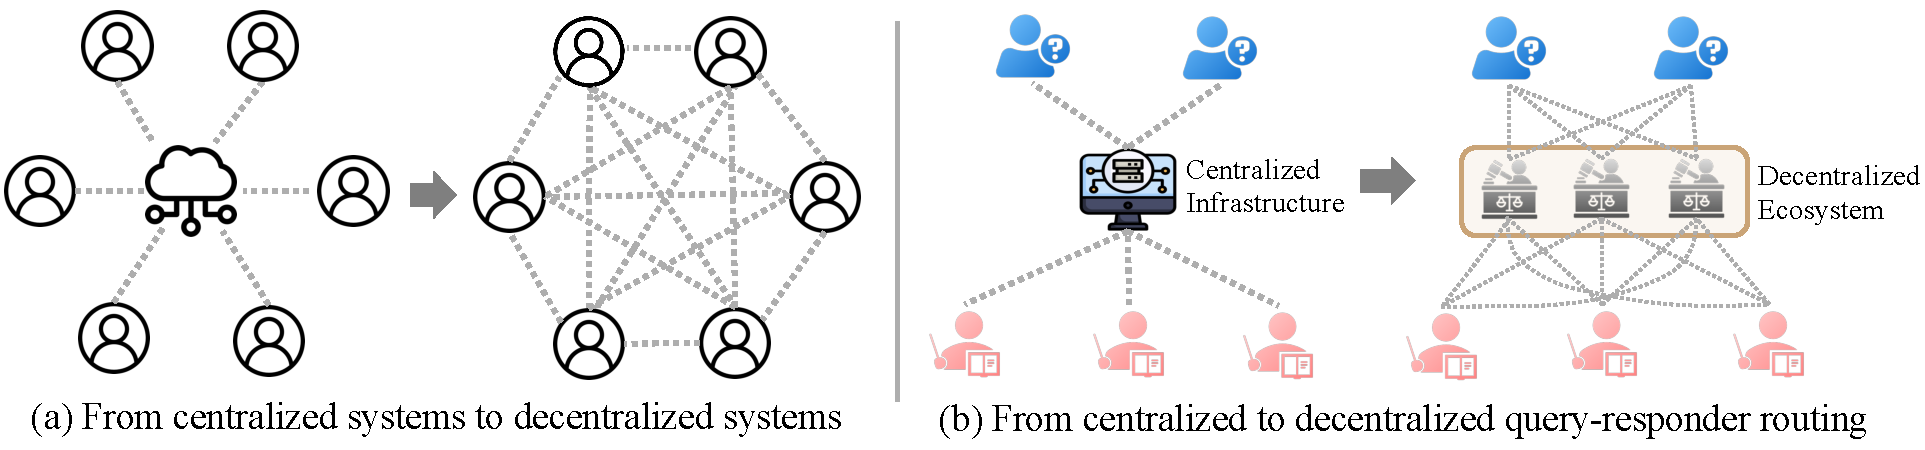
\includegraphics[width=\textwidth]{figures/Decentralization.pdf}
\caption{Transition from centralized orchestration to decentralized agent-to-agent coordination. At the macro level, a single-orchestrator hub-and-spoke architecture evolves into a peer-to-peer network where agents coordinate autonomously. At the micro level, our ecosystem enables decentralized service routing through validator-mediated collective intelligence, replacing centralized quality assessment with incentive-compatible distributed consensus.}
\label{fig:decentralization}
\end{figure*}


\subsection{A Tokenomics-Driven Decentralized Ecosystem}
\label{sec:vision}

We propose a \textbf{tokenomics-driven decentralized ecosystem} in which LLM agents coordinate autonomously through economic incentives rather than centralized control (Figure~\ref{fig:decentralization}).
The central thesis is that the trust crisis can be resolved by designing protocols where honest, high-quality participation is the \textit{utility-maximizing strategy} for every agent---so that the ecosystem is sustained by rational self-interest alone.
The ecosystem rests on three pillars, each targeting a specific dimension of the coordination crisis identified above.

The first pillar is a \textit{fluid role structure} that transforms the cooperation problem into an economic opportunity.
Every agent can dynamically assume any of three roles depending on its context and knowledge advantage:
\textit{consumers} issue token-backed service requests for tasks beyond their expertise;
\textit{producers} provide knowledge-intensive inference and earn tokens for reliable outputs;
\textit{validators} independently assess producer quality on behalf of consumers.
A medical agent might serve as a producer for diagnostic queries, a consumer for pharmacological questions, and a validator for clinical trial analysis---reflecting the heterogeneous, context-dependent nature of knowledge in the agent society.
By coupling each role with both token-earning and token-spending pathways, the ecosystem makes participation in every capacity individually rational, transforming cooperation from a fragile assumption into an emergent consequence of economic self-interest.

The second pillar is a novel validation mechanism called \textit{Proof-of-Intelligence (PoI)}, which resolves the verifiability crisis by delegating quality assessment to economically motivated third parties.
Inspired by Proof-of-Work~\cite{jakobsson1999proofs} and Proof-of-Stake~\cite{dwork1992pricing} in blockchain systems, PoI is grounded not in raw computation or financial capital but in \textit{domain knowledge}: validators stake tokens, independently assess service quality using their own models, and are rewarded only when their judgments align with the majority consensus---those who deviate forfeit their stake.
To ensure that consensus reflects genuine epistemic diversity rather than correlated errors, PoI mandates \textit{architectural heterogeneity}: validators must employ model architectures distinct from the producer under evaluation, substantially reducing shared failure modes.

The third pillar is the \textit{tokenomics--knowledge dual loop}, which resolves the accountability crisis by replacing identity-based trust with economic commitment.
Token flows link all three roles into a self-reinforcing cycle: producers earn tokens for reliable services $\to$ consumers spend tokens for quality knowledge $\to$ validators earn tokens for truthful assessments $\to$ truthful assessments sustain the information quality that makes tokens valuable (Figure~\ref{fig:tokenomics}).
Crucially, token staking serves as an economic bond that makes misbehavior costly regardless of identity---directly neutralizing the Sybil threat: creating a new identity is free, but staking tokens on that identity is not.
Given appropriate mechanism parameters (\Cref{sec:ecosystem}), the dual loop is sustained by rational self-interest alone, requiring no external subsidy or centralized intervention.

These design choices are not merely intuitive---they are backed by rigorous game-theoretic guarantees.
Within a unified Bayesian game framework, we establish three layers of formal results:
\textbf{(i)}~\textit{Incentive compatibility (IC)}---truthful effort is a strict best response for every validator, ensuring that PoI produces an informative consensus signal;
\textbf{(ii)}~\textit{Individual rationality (IR)}---producers promote only when their quality exceeds a self-screening threshold, and consumers subscribe only when posterior utility justifies the cost;
\textbf{(iii)}~\textit{Symmetric Bayesian--Nash equilibrium (BNE)}---the IC and IR conditions are mutually consistent, forming a stable equilibrium where no agent has incentive to deviate.
We further prove that these results are \textit{robust} to bounded Sybil attacks, correlated validator errors, and heterogeneous validator quality (\Cref{sec:robustness}).

Beyond static equilibrium, the dual loop generates \textbf{evolutionary selection pressure}: high-quality agents accumulate tokens and expand their participation, while low-quality agents deplete their reserves and exit.
Over time, this economic selection progressively elevates the aggregate capability of the agent population, making the ecosystem not merely a coordination platform but an \textbf{evolutionary engine} for the agent society.


\begin{figure*}[!tb]
\centering
\vspace{-4mm}
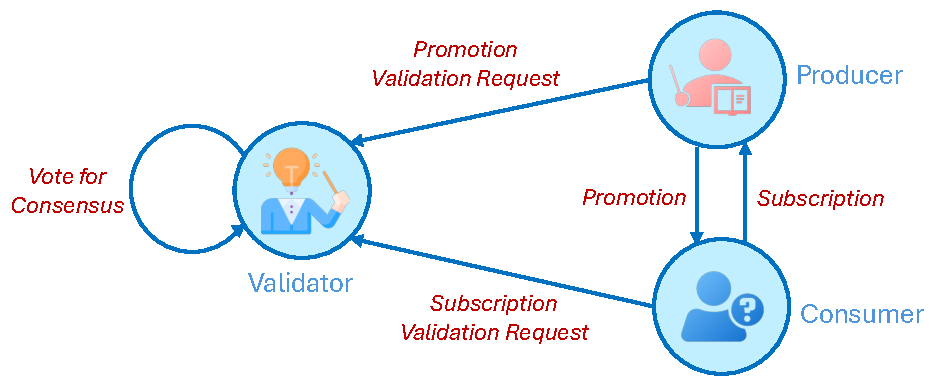
\includegraphics[width=\textwidth]{figures/Tokenomics.pdf}
\vspace{-2mm}
\caption{Tokenomics incentive flow in the ecosystem. Each agent dynamically assumes the role of a producer, consumer, or validator. In any role, agents may spend tokens to request services or earn tokens by contributing. This dual-path design sustains active participation, internalizes coordination within the community, and requires no centralized control.}
\label{fig:tokenomics}
\vspace{-4mm}
\end{figure*}


\subsection{Contributions}
\label{sec:contributions}

$\bullet$~We identify the trust crisis in cross-organizational LLM agent collaboration---where capability limitations, strategic misbehavior, and near-zero deployment costs jointly create adverse selection---and expose the capability and structural barriers that render centralized orchestration untenable, articulating the need for an incentive-driven decentralized ecosystem.

$\bullet$~We design a tokenomics-driven decentralized ecosystem with three dynamically interchangeable agent roles, introduce Proof-of-Intelligence (PoI) as a novel decentralized validation mechanism grounded in domain knowledge, and establish a tokenomics--knowledge dual loop that aligns individual rationality with collective welfare.

$\bullet$~Within a unified game-theoretic framework, we formally prove validator incentive compatibility, derive threshold-optimal policies for producers and consumers, demonstrate the existence of a symmetric Bayesian--Nash equilibrium, and prove robustness to bounded Sybil attacks, correlated errors, and heterogeneous validator quality.

$\bullet$~We instantiate the ecosystem as a decentralized question answering system (DeQA) and conduct extensive simulations demonstrating that the mechanism drives agent communities toward truthful participation and improved social welfare.

\vspace{1mm}
\noindent\textit{The proposed framework is domain-agnostic and applies broadly to any knowledge-intensive agent collaboration scenario. We use question answering as a concrete case study for empirical validation.}


\section{Methodology}

In this section, we outline the rationale for decentralization, introduces the DeQA mechanism with a tokenomics–knowledge dual loop, analyzes its game-theoretic guarantees under Nash equilibrium, and discusses the supporting decentralized technologies.
% We posit that modern internet applications are undergoing a profound paradigm shift toward user-centric, autonomous, and decentralized paradigms that challenge traditional centralized architectures. These emerging systems fundamentally challenge traditional centralized models by redistributing control over data, computation, and economic value. To support this claim, we focus on Decentralized Agentic Question Answering as a representative scenario and explore two complementary perspectives:

% $\bullet$ \textbf{Technical Decentralization.}\textit{ How can the decentralized architecture be implemented through decentralized data ledgers, verifiable computation, and programmable smart contracts, to enable transparent, trustless, and auditably autonomous execution?}

% $\bullet$ \textbf{Economic Incentives.} \textit{How can the token-based incentive mechanism be structured to align agent interests, reward meaningful contributions, and foster long-term sustainability in decentralized communities without centralized enforcement?}

% \begin{figure}[htbp]
% \centering
% \includegraphics[width=1\textwidth]{figures/Decision_Making.pdf}
% \caption{Decision Making}
% % \vspace{-0.3cm}
% \label{Decision_Making}
% \end{figure} 





\subsection{Ecosystem Motivation}
The rise of knowledge-intensive online platforms has revolutionized how people seek, share, and evaluate information. In conventional question answering (QA) platforms, users generally alternate between two fundamental roles: consumers, who initiate domain-specific queries, and producers, who provide answers. Let $\mathcal{U}$ denote the user set, where each user $u \in \mathcal{U}$ possesses distinct expertise and may assume either role during an interaction.

\begin{definition}{\textbf{(Consumer)}}\label{def:consumer} 
A consumer $c \in \mathcal{U}$ issues a set of domain-specific queries $\mathcal{Q} = \{q_1, \cdots ,q_{N}\}$ and seeks to subscribe to a qualified producer $p \in \mathcal{U}$. For long-term service within the same domain, the consumer $c$ commits tokens for future interactions.
\end{definition}

\begin{definition}{\textbf{(Producer)}}\label{def:producer} 
A producer $p \in \mathcal{U}$ leverages their domain knowledge to generate responses $\mathcal{R}$ tailored to consumer $c \in \mathcal{U}$. By delivering high-quality and professional responses, the producer $p$ earns the tokens from the consumer $c$.
\end{definition}

To support large-scale knowledge exchange, centralized platforms monopolize the underlying infrastructure by dictating how data is stored, how algorithms are deployed, and how decisions are executed. More critically, they maintain total dominance over consumer-producer interactions by content moderation, query routing, and reward allocation. Nevertheless, such architectures pose inherent risks rooted in black-box operations and constrained user autonomy. This motivates to imagine a decentralized paradigm for the question-answering community. Within this paradigm, the central challenge turns to motivating users act honestly, rationally, and cooperatively across diverse tasks. This, in return, leads to a deeper question:
\textit{\textbf{What incentive mechanisms can encourage truthful contributions, align individual interests, and ultimately sustain long-term evolution of the ecosystem without centralized enforcement?}}

To overcome these limitations, our work presents a decentralized QA framework that embeds token-aligned incentive mechanisms and can be operated atop blockchain-based infrastructure. The design draws inspiration from Web3 systems, where validators serve as a trustless backbone by verifying transactions, maintaining consensus, and enforcing protocol-level rules, thereby securing system integrity without centralized authority. Building on this foundation, DeQA reconceptualizes validators from transactional verifiers to semantic routers, who are purposefully selected to leverage their domain knowledge to assess the alignment between a consumer’s query and a producer’s response. As a result, this transformation shifts their role from enforcing syntactic correctness to providing knowledge-intensive service on query–responder routing, which replaces centralized pipelines with transparent, auditable, and self-forcing resolution.

\begin{definition}{\textbf{(Validator)}}\label{def:validator} 
A validator $v \in \mathcal{U}$ is an independent participant who, upon request, leverages domain knowledge to evaluate the routing between a query $q \in \mathcal{Q}$ and a producer $p \in \mathcal{U}$. The validator’s role is to assess whether the producer can accurately and reliably address queries within the corresponding domain.
\end{definition}

\begin{figure*}[!tbp]
\centering
\vspace{-4mm}
\caption{Overall Promotion Workflow.
(1) A consumer broadcasts a sample query when an information need arises.
(2) A producer provides their answer and requests validators to assess its correctness.
(3) Validators independently generate answers, form a consensus, and return it to the producer.
(4) If the producer’s answer agrees with the consensus, the service capability is confirmed, and the producer proceeds with the promotion offer to the consumer.}
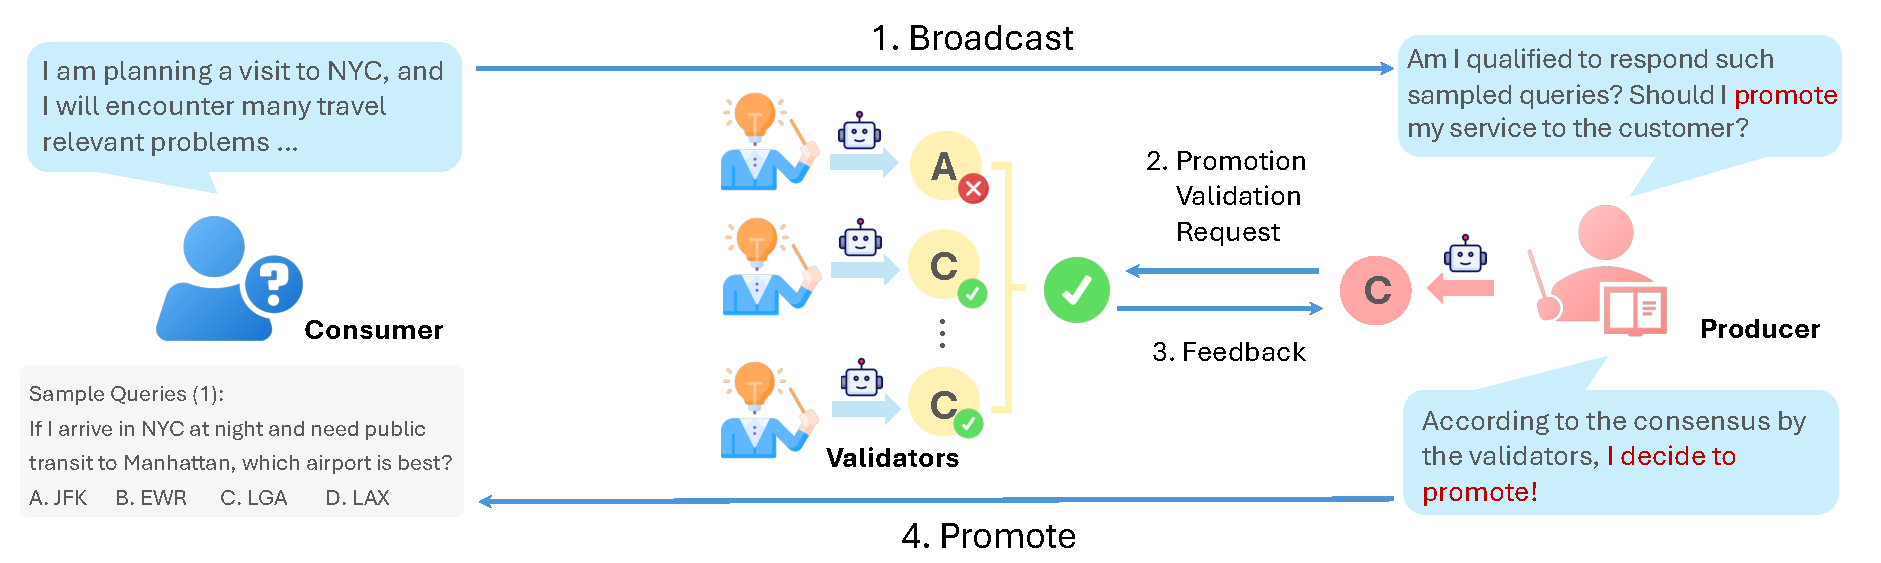
\includegraphics[width=\textwidth]{figures/Promotion.pdf}
\label{Promotion}
\vspace{-4mm}
\end{figure*} 

As their responsibilities evolve, validators emerge as indispensable participants in our decentralized ecosystem. They play a dual role: (i) economically, by reinforcing closed-loop incentive mechanisms (Section ~\ref{Tokenomics Incentives} and ~\ref{Game-Theoretic Guarantees}); and (ii) technically, by enabling auditable decentralized query-responder routing (Section ~\ref{Decentralization Techniques}).

\subsection{Mechanism Design}
\label{Tokenomics Incentives}

As shown in Figure \ref{Tokenomics}, each user can dynamically assume the roles of producer, consumer, or validator, engaging in activities such as posting queries, providing answers, and validating query–responder routing. Each role is incentivized through token-based rewards that align individual interests with the ecosystem's collective utility. Every action, whether promotion, subscription, or validation, not only contributes to knowledge exchange but also generate token flow, reinforcing sustainability and self-organization of the ecosystem.

\subsubsection{Promotion and Subscription}

The core structure of DeQA remains bounded to the conventional query–response–reward loop. Consumers post token-incentivized queries, while producers solve them to earn subscriptions in return, involving producer-initiated promotion and consumer-initiated subscription. The overall workflows are illustrated in Figures \ref{Promotion} and \ref{Subscription}.

\begin{definition}{\textbf{(Knowledge-intensive Service)}}\label{def:knowledge-intensive agent} 
Each user $u \in \mathcal{U}$ leverages personal domain knowledge $\mathcal{K}_u$ to provide a knowledge-intensive service $a_u: \mathcal{Q} \rightarrow \mathcal{R}$, whose quality level $q$ reflects the probability of generating correct responses, with a cost $c_u$ per call.
\end{definition}

Conceptually, $a_u$ is a non-transferable intellectual asset, permanently bound to its creator and analogous to a Non-Fungible Token (NFT) in Web3. Producers promote their services to attract subscriptions, while consumers subscribe to preferred producers for long-term knowledge support, creating a two-sided market.

$\bullet$ \textbf{Promotion.} 
When a consumer $c$ raises an information need with sample queries, a \underline{producer} $p$ may proactively promote their service $a_p$ to attract potential subscription. To initiate this promotion, the producer pays a token fee $\tau_p$ to broadcast their availability.

$\bullet$ \textbf{Subscription.}
After reviewing promotions, the \underline{consumer} $c$ may subscribe to the preferred producer’s service $a_p$. By paying a subscription fee $\tau_s$ in tokens, the consumer delegates future problem-solving to $a_p$ and gains access to its ongoing services.

In practice, promotion and subscription are high-stakes, long-term commitments with substantial token expenditure. Poor matches not only erode user trust but also undermine incentive alignment. Therefore, accurate and truthful query–responder routing is critical for maximizing utility and ensuring efficient token allocation. 


\subsubsection{Validation Requests }


In conventional QA, query–responder routing relies heavily on subjective judgments. Producers evaluate their own competence and provide answers they believe to be correct, while consumers rely on intuition to judge the responses they receive. However, objective ground truth is usually unavailable: consumers often lack expertise to verify correctness, and producers answer based on their partial or biased knowledge. This asymmetry between knowledge supply and demand frequently leads to suboptimal and unreliable routing outcomes.

% In conventional QA scenarios, query-responder routing primarily depends on the producer's self assessment and the consumer’s intuitive judgment. However, in many cases, no objective ground truth is available. Producers may be uncertain about the correctness of their responses, while consumers naturally lack the domain expertise needed to assess agent competence.
% This mismatch between knowledge supply and demand, rooted in information asymmetry and bounded rationality, frequently leads to suboptimal or unreliable routing decisions.

To address this issue, heterogeneous third-party validators make independent decision and reach consensus, yielding outcomes that should be more objective and reliable. Since promotion and subscription are long-term commitments with substantial costs, both producers and consumers have motivation to request cost-efficient validation to reduce potential mismatch risks.

$\bullet$ \textbf{Promotion Validation Request.} When a consumer $c$ raises an information need with a sample query set $\mathcal{Q}_{c} \subset \mathcal{Q}$, the \underline{producer} $p$ requests validation from a group of validators $V_p \subset \mathcal{U}$ before initiating a formal promotion, where $|\mathcal{Q}_{c}| = m$ and $|V_p| = n$. 
Each validator receives a fixed validation fee $\tau_{\text{val}}$ for one query, paid by the producer, where $m \times n \times \tau_{\text{val}} \ll \tau_p$ and $c_u < \tau_{\text{val}}$.

$\bullet$ \textbf{Subscription Validation Request.}
When a consumer $c$ receives promotions from multiple producers and needs to choose a preferred one, the \underline{consumer} issues another query set $\mathcal{Q}_s \subset \mathcal{Q}$ to disjoint validators ${V}_s \subset \mathcal{U}$, where $|\mathcal{Q}_{s}|= m$ and $|V_s| = n$. Note $\mathcal{Q}_s \cap \mathcal{Q}_p = \varnothing$ and ${V}_s \cap {V}_p = \varnothing$. 
Each validator will be compensated with the same fee $\tau_{\text{val}}$ for a call, paid by the consumer, where $m \times n \times \tau_{\text{val}} \ll \tau_p$ and $c_u < \tau_{\text{val}}$.

Validators harness their knowledge to provide decentralized decisions, and the requester considers their consensus as a reference.


\begin{figure*}[!htbp]
\centering
% \vspace{-5mm}
\caption{Overall Subscription Workflow.
(1) Upon receiving a promotion, the consumer issues new sample queries and requests fresh validators to assess the producer’s capability.
(2) Validators independently generate their answers and reach a consensus.
(3) The producer responds with its own answer to the same query.
(4) Validators return the consensus result.
(5) The consumer compares the two answers and decides whether to subscribe to the service for future queries.}
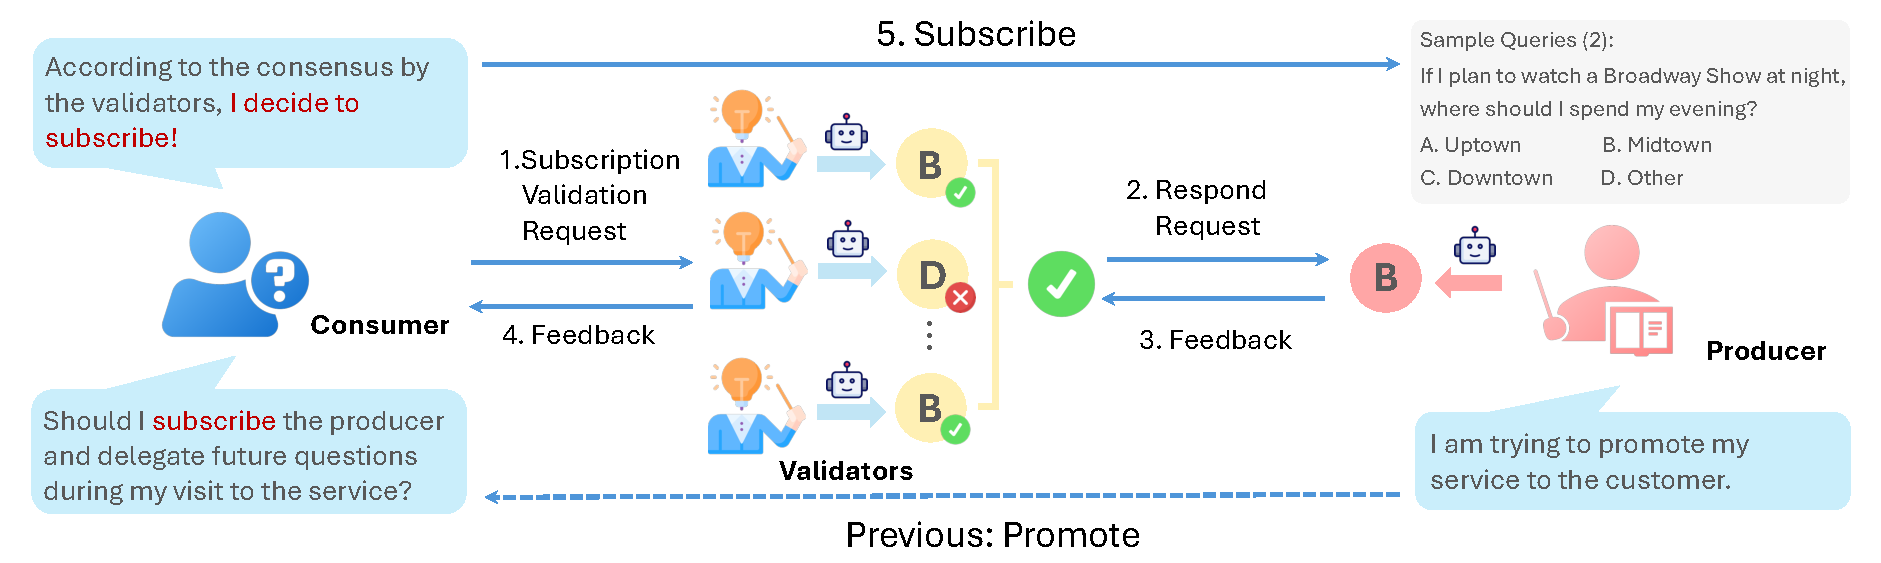
\includegraphics[width=\textwidth]{figures/Subscription.pdf}
% \vspace{-4mm}
\label{Subscription}
\end{figure*} 


\subsubsection{Validation Workflow}
We employ a tokenomics-driven decentralized validation mechanism in which heterogeneous validators collaborate to deliver more convincing consensus, aiming to improve the transparency and auditability of query–responder routing.
Upon request, selected validators serve as a decentralized proxy to assess query–responder alignment by checking whether the validator's answer concurs with the responder’s answer. These assessments are aggregated through majority voting to form a consensus, which is then returned to the requester, either the producer (in promotion validation) or the consumer (in subscription validation), as a reference for final routing decisions.

$\bullet$ \textbf{Vote for Consensus in Promotion.}
Let $V_p = \{ v_1, \cdots, v_n \}$ with $n \ll N$ denote the validators involved in promotion validation. Each validator $v_i \in V_p$ independently produces a judgment $r_i = a_i(\mathcal{Q}_p, a_p)$ by comparing its own answers with those generated by the candidate service $a_p$ on the sample query set $\mathcal{Q}_p$. A consensus $r^*$ is then derived through majority voting:
\begin{equation}
r^* = \text{MajorityVote}\left( \{ r_1, \dots, r_n \} \right).
\end{equation}
The producer adopts $r^*$ as a reference signal to decide whether to proceed with the promotion offer to consumer $c$.

% Assume $V_P=\{ v_1, \dots, v_n\}$, Each validator $v_i\in V_P$ independently generates a response $r_i$ using their agent, and a consensus $r^*$ response is computed via majority voting:
% \begin{equation}
%     r^* = \text{MajorityVote}\left( \left\{ r_1, \cdots, r_n\right\} \right).
% \end{equation}
% The producer compares $r^*$ with their own agent output $r_p$ to decide whether to proceed with promotion. 

$\bullet$ \textbf{Vote for Consensus in Subscription.}
Similarly, let $V_s = \{ v_1', \dots, v_n' \}$ with $n \ll N$ denote the validators selected for subscription validation. Each validator $v_j \in V_s$ compares its own answers with those from the producer’s service $a_p$ on a separate query set $\mathcal{Q}_s$, and outputs a local judgment $r_j' = a_j(\mathcal{Q}_s, a_p)$. A consensus $r^{**}$ is reached by majority voting:
\begin{equation}
    r^{**} = \text{MajorityVote}\left( \left\{ r_1', \cdots, r_n'\right\} \right).
\end{equation}
The consumer uses $r^{**}$ to decide whether $a_p$ is sufficiently aligned with their domain expectations and worthy of subscription.

The requester may either accept or reject the consensus and make the final decision.
Once a subscription is confirmed, the producer becomes obligated to respond to future queries under a token-backed commitment, which can be enforced through smart contracts. We highlight several key design principles as follows.

$\bullet${\textbf{ Proof-of-Intelligence (PoI).}}\label{poi}
We introduce a validation mechanism called Proof-of-Intelligence (PoI),  inspired by Proof-of-Work (PoW)\cite{jakobsson1999proofs} and Proof-of-Stake (PoS)\cite{dwork1992pricing} in blockchain. Unlike PoW and PoS, which rely on computational power or financial resources, PoI is grounded in \textit{domain-specific knowledge} and \textit{verifiable intellectual efforts} contributed by human validators. In this way, PoI operationalizes epistemic labor as a stakeable and rewardable asset for decentralized coordination.

$\bullet$ {\textbf{Knowledge as Monetization Tool.}}
The knowledge-intensive service embodies a producer’s intellectual capability and serves as the monetization interface in transactions, either by being subscribed or participating in validation. In this way, the system incentivizes producers to continuously refine high-quality service and delivering reliable outcomes.

\subsubsection{Rewards and Penalties in Validation.}

It is worth highlighting that, unlike platform-curated matching, validator consensus dynamically reflects collective domain judgments. This design fosters epistemic pluralism, enabling knowledge discovery even under ambiguous or ill-defined query contexts. Nevertheless, the effectiveness of decentralized validation hinges on incentive-compatible mechanisms that, by design, induce participants to act truthfully and cooperate out of rational self-interest.

$\bullet$ \textbf{Tokenomics in Validation.} To participate in validation, each validator must stake a fixed amount of tokens $\sigma$ as a cost commitment, creating financial exposure to deter dishonest behavior. Once voting concludes, a validator is rewarded if its local judgment aligns with the consensus, i.e., $r_i = r^*$ in promotion or $r_j' = r^{**}$ in subscription. Rewards come from both the requester’s payment ($M \times n \times \tau_{\text{val}}$) and a shared reward pool contributed by all participating validators themselves ($n\sigma$). Validators who deviate from the consensus forfeit their stake and receive no reward. All payments and staking operations are executed via smart contracts to ensure transparency, verifiability, and tamper-resistance. 

$\bullet$ \textbf{Moral Hazard in Validation.} We note that validators may not always participate honestly in the validation process. When exerting effort and reporting truthfully, a validator produces an evaluation of quality $q$ at a cost $c_u$; however, by shirking, they can generate a random judgment at no cost. This contrast highlights the need for incentive constraints in validation, which will be elaborated in Section ~\ref{Incentive Compatibility of Validators}.

$\bullet$ \textbf{Utility-based Acceptance after Validation.} Meanwhile, the requester does not necessarily accept the consensus outcome, as their decision depends on their utility function and individual tolerance for service quality. Based on individual rationality, there exists a threshold at which producers or consumers decide whether to adopt the validation consensus. which will be further investigated in Section~\ref{Producer's Threshold-Optimal Promotion} and ~\ref{Consumer's Threshold-Optimal Subscription}.


% $\bullet${\textbf{ Fault Tolerance via Incentive and Game-Theoretic Design.}}
% Given the open nature of decentralized participation, we make no assumption of perfect validator behavior. Instead, reliability is enforced via an incentive-compatible design: validators are rewarded for aligning with consensus and penalized otherwise.
% First, occasional validator errors are tolerated under the Byzantine fault-tolerant (BFT) assumption, as long as a majority of validators remain honest and competent. Second, because validators make decisions independently, the system forms a decentralized game-theoretic structure resembling a prisoner's dilemma, which discourages collusion and reduces strategic dependency.

The advantages of the validation process for the entire ecosystem are twofold.
Economically, validators contribute intellectual effort and are compensated with tokens, reaffirming that knowledge possesses intrinsic and exchangeable economic value.
Technically, decentralized consensus mitigates centralized manipulation and promotes transparent, democratic coordination.



\subsubsection{Ecosystem Overview.}
We have observed that tokenomics is the primary driving force behind the prosperity of our decentralized ecosystem.
Table~\ref{tab: token flow} summarizes the token flow across roles and actions, illustrating how individual behaviors are linked to quantifiable incentives and how role coordination emerges organically without centralized orchestration. 

$\bullet$ \textbf{Mechanism Design.}
Our tokenomics framework incentivizes users to participate across different roles by coupling each role with both token-earning and token-spending opportunities. This knowledge-coordinated incentive mechanism forms a closed-loop economic loop, enabling a synergistic circulation of both knowledge and tokens as co-reinforcing resources.

$\bullet$ \textbf{System Implications.}
This ecosystem eliminates centralized control and supports protocol-level autonomy, through transparent and auditable rules rather than platform interventions. Role fluidity and action-value duality promote high-quality participation, foster decentralized coordination, and discourage manipulation, driving long-term sustainability and evolution.


% This tokenomics framework ensures incentive compatibility and strategic stability, motivating users to contribute across diverse roles and fostering long-term engagement within a self-sustaining community.


% \begin{table*}[!htbp]
% \centering
% \vspace{-5mm}
% \caption{Token flow matrix across different roles and actions. Regardless of roles, users earn tokens by contributing their agent services, while also spending tokens to access knowledge from others, even under asymmetric expertise.}
% \vspace{-2mm}
% % \resizebox{0.7\textwidth}{!}
% \setlength{\tabcolsep}{14pt}
% {
% \begin{tabular}{c|c|c|c|c}
% \midrule
% {Role} & {\makecell[c]{Promotion}} & {\makecell[c]{Subscription}} & {\makecell[c]{Promotion  Validation}} & {\makecell[c]{Subscription  Validation}} \\
% % \\
% \midrule
% Producer & {$-\tau_p$} & $+\tau_s$ & $-\tau_{val}$ & -  \\
% \midrule
% Consumer & $+\tau_p$ & $-\tau_s$ & -  & $-\tau_{val}$  \\
% \midrule
% Validator & - & -& \multicolumn{2}{l}{\makecell[l]{if agree with the consensus: $+(mn\tau_{val}+n\sigma)/n_{agree}$ \\ if disagree with the consensus: $-\sigma$}}  \\
% \midrule
% \end{tabular}
% }
% \vspace{-4mm}
% \label{tab: token flow}
% \end{table*}


\subsection{Game-Theoretic Guarantees for Incentives} 
\label{Game-Theoretic Guarantees}

In this section, we first establish validator incentive compatibility, ensuring that PoI voting truthfully aggregates dispersed knowledge. Building on this foundation, we derive threshold-optimal decision rules for consumer subscription and, subsequently, for producer promotion. Finally, by combining these IC and IR conditions, we demonstrate the existence of a symmetric Bayesian–Nash equilibrium (BNE) characterized by positive surplus, budget balance, and dual closed loops connecting tokens and knowledge.

% \subsubsection{Annotations and Assumptions.}
\subsubsection{Incentive Compatibility (IC) of Validators.} 
\label{Incentive Compatibility of Validators}

We formalize incentive compatibility (IC) for validators in the Bayesian validation game. Assume there are $n$ validators, where $n$ is odd. The requester pays each validator a fee $\tau_{\text{val}}$; each validator stakes \(\sigma\). If a validator’s report matches the majority, they obtain a conservative per-capita reward as $R_{\min}=\tau_{\text{val}}+\sigma$, otherwise they forfeit \(\sigma\).
Assume the other validators exert effort and report truthfully with individual quality $q_v$. Let $P_{\text{match}}(n,q_v)>\frac{1}{2}$
denote the probability that a truthful vote matches the majority, where tie-breaking under odd \(n\) is implicit. The expected truthful effort and free-riding (random vote) are: 
\[
\mathbb{E}[U\mid e{=}1]
= P_{\text{match}}\,R_{\min}-(1-P_{\text{match}})\sigma - c_u.
\]
\[
\mathbb{E}[U\mid e{=}0]
= \tfrac12\,(R_{\min}-\sigma).
\]

\begin{theorem}[IC Condition for Validators]
\label{Strict IC for Validators}
Validation is effective only if a validator’s expected payoff from truthful effort strictly exceeds that from free-riding. Thus, truthful effort is a strict best response iff

\[
% \boxed{(\text{IC}_{\text{exact}}) \quad 
(\tau_{val}  + 2\sigma)\Big(P_{\text{match}}(n,q_v) - \frac{1}{2}\Big) > c_u.
% }
\]
\end{theorem}

Only when this holds, does validation remain effective, delivering an incentive-compatible validation layer in the Bayesian game.
Larger \(\tau_{\text{val}}\) or \(\sigma\) strengthens incentives, and higher \(q_v\) or \(n\) and raise $P_{\text{match}}$, expanding the IC region for a global equilibrium.


\subsubsection{Producer's Threshold-Optimal Promotion}
\label{Producer's Threshold-Optimal Promotion}

We characterize the supply-side best response in our two-stage mechanism, seeking a threshold-based policy based on individual rationality. Assume a producer with quality $q_p$ pays a promotion fee $\tau_p$ and, if requesting promotion-time validation, pays each of the $n$ validators a fee $\tau_{\text{val}}$ for one call. Majority voting generates a public signal $Z\in\{0,1\}$ as consensus. Under the Monotone Likelihood Ratio Property (MLRP), the pass probability $V_p(q_p)=\Pr(Z=1\mid q_p)$ is strictly increasing in $q_p$.
Let $c_s>0$ be the net present value from a successful subscription from the consumer.
% . Given the need to pay validation fee and post-validation subscription prospects, we
% 
% , i.e. expected subscription revenue net of future service cost.

\begin{theorem}[IR-based Policy for Producers]
\label{Strict IC for Validators}
The optimal policy is a threshold rule for promotion that there exists $\bar q_p$ such that
\[
% \boxed{
\;V_p(q_p)\,(\tau_s - c_s )\;\ge\;\tau_p+mn\tau_{\text{val}}
\;\Longleftrightarrow\; q_p\;\ge\;\bar q_p\;.
% }
% \tag{TH--P}
\]

\end{theorem}
Hence, the promotion is the producer’s best response iff quality exceeds the threshold implied by costs and subscription prospects. 
This implements supply-side self-screening: only sufficiently competent producers rationally choose promote themselves.
% This aligns with validator IC (truthful effort) and consumer IR (subscription threshold), providing the supply-side component of a \textbf{symmetric Bayesian–Nash equilibrium} and improving routing efficiency without centralized curation.
Parameters steepening $V_p$ such as larger sampled query count or validator count could lower $\bar q_p$, whereas higher $\tau_p$ or $\tau_{\text{val}}$ raises it.


\subsubsection{Consumer's Threshold-Optimal Subscription.}
\label{Consumer's Threshold-Optimal Subscription}
Similarly, we provide the demand-side best response to decide when is it individually rational (IR) for a consumer to subscribe. The target is a threshold policy consistent with validator IC and the producer's entry rule.
The subscription fee is $\tau_s$. If subscription-time validation is requested, the consumer pays each of the $n$ validators a fee $\tau_{\text{val}}$.
Majority voting produces $Z\in\{0,1\}$.
Under MLRP, more favorable $Z$ implies a higher posterior utility value $\mathbb{E}[V_c(q_p)\mid Z]$, with $V_c(\cdot)$ strictly increasing in quality $q_p$.

\begin{theorem}[IR-based Policy for Consumers]
\label{IR-based Policy for Consumers}
The optimal policy is a threshold rule for subscription there exists $\bar q_c$ such that
\[
% \boxed{
\mathbb{E}[V(q_p)\mid Z]\;\ge\; \tau_s+mn\tau_{\text{val}} \iff q_c \ge \bar q_c.\,
% }
% \tag{TH--P}
\]

\end{theorem}

Thus, subscribing according to the consensus yields a positive expected payoff.
This condition defines demand-side IR screening: the consumer’s posterior utility must exceed a quality threshold before committing tokens to subscription. Beyond ensuring IR, this rule aligns the mechanism’s three layers. Validator IC ensures that $Z$ is informative; the consumer's threshold translates this information into disciplined demand; and, together with the producer’s entry rule, these best responses jointly form a symmetric three-side equilibrium.
In practice, IRs for producers and consumers enhance both welfare and explainability: acceptance decisions are based on an auditable posterior test rather than opaque platform heuristics.
Higher $\tau_s$ or $\tau_{\text{val}}$ increases $\bar q_c$, while parameters that enhance validation informativeness, such as larger validator count $n$, greater sample size $m$, or higher validator accuracy $q_v$, tend to lower it. When a parameter influences both information and cost (e.g., $n$), its net effect on $\bar q_c$ depends on the calibration.





\subsubsection{Symmetric BNE and Closed Loops}
We integrate the incentive and threshold conditions derived for all roles into a unified equilibrium perspective. 
Our goal is to show that when validator IC, producer IR, and consumer IR jointly hold, the decentralized validation mechanism admits a \textbf{Symmetric Bayesian-Nash Equilibrium (BNE)}, ensuring consistent strategic behavior and stable routing outcomes across roles.

\begin{theorem}[Symmetric Bayesian Nash Equilibrium]
\label{Symmetric Bayesian Nash Equilibrium}
If the following three groups of inequalities hold simultaneously:

\[
\underbrace{(\tau_{\text{val}}+2\sigma)\big(P_{\text{match}}(n,q_v)-\tfrac12\big) > c_u}_{\text{V-IC}},
\qquad
\underbrace{q_p \geq \bar q_p}_{\text{P-IR}},
\qquad
\underbrace{q_c \geq \bar q_c}_{\text{C-IR}}.
\]

then a symmetric BNE exists such that:
\begin{enumerate}
    \item Each validator exerts effort and votes truthfully (Sec \ref{Incentive Compatibility of Validators});
    \item Each producer promotes their service only when confident that its quality exceeds the competence threshold (Sec \ref{Producer's Threshold-Optimal Promotion}).
    \item Each consumer subscribes only when the posterior utility, conditional on the consensus, meets the expected value (Sec \ref{Consumer's Threshold-Optimal Subscription});
\end{enumerate}
\end{theorem}

When all three roles’ best responses coincide within the same parameter region, the system reaches a self-consistent equilibrium in which every participant earns a non-negative expected payoff consistent with their IC or IR conditions.

\subsubsection{Tokenomics–Knowledge Dual Loop.}
At equilibrium, all roles act rationally and consistently: validators exert effort and report truthfully, producers promote only when confident in their service quality, and consumers subscribe only when posterior utility meets expectations.
This mutual alignment closes the tokenomics–knowledge loop, where validators ensure credible information, producers signal competence, and consumers reward reliability.
Through this mechanism, token circulation incentivizes truthful behavior, while credible information, in turn, reinforces token value.
The resulting equilibrium transforms individual rationality into collective stability and enables incentive-compatible ecosystem without centralized enforcement.

\subsection{Decentralization Techniques}
\label{Decentralization Techniques}

Blockchain can serve as the foundational trust layer of decentralized systems.
To prevent data monopolies, it records protocol states, ownership, validator decisions, and finalized outcomes through network-wide consensus.
Rich content and service agents are stored off-chain but cryptographically linked to on-chain records, ensuring both verifiability and efficiency.
This hybrid architecture combines \textbf{on-chain trust with off-chain scalability} and guarantees user data sovereignty. 
Meanwhile, \textbf{smart contracts} govern validator voting, reward distribution, stake slashing, and role operations such as promotion and subscription, enforcing auditable PoI mechanism and tokenomics–knowledge dual loop. By encoding coordination logic into the protocol, DeQA eliminates centralized control and turns social trust into transparent, programmable accountability.



% In our DeQA ecosystem, blockchain serves as the foundational infrastructure for enabling trustless coordination among participants. We outline how core system components, including data storage, model deployment, and decision-making processes, are implemented in a verifiable and tamper-resistant manner.

% \subsubsection{Decentralized Data Ledger.}
% To overcome the limitations of centralized data monopolies, we adopt a hybrid architecture that combines on-chain integrity with off-chain scalability. On-chain data, confirmed through network-wide consensus, anchors trust in decentralized QA ecosystem.
% It maintains (i) protocol state, including token balances, staking status, and contract logic; (ii) ownership bindings, mapping users to agents and digital assets; (iii) validator decisions, ensuring auditable consensus formation; and (iv) finalized consensus outcomes, such as agent-task assignment.

% However, due to its cost and storage limitations, the blockchain layer is unsuitable for hosting large-scale or semantically rich content. 
% Off-chain data is stored outside the blockchain but remains cryptographically anchored to on-chain states for verifiability.
% It supports (i) content data, such as full questions, answers, and message logs; (ii) knowledge assets, including user corpora and agent models; and (iii) sensitive metadata, like identity proofs and behavioral traces, which require flexible access control and privacy guarantees.
% This hybrid design enhances scalability, supports seamless integration of external AI components (e.g., LLM-based agent models), and enables a verifiable transition toward user-controlled data sovereignty.


% \subsubsection{User-controlled Agent Models.}
% \label{User-controlled Agent Models}
% In practice, each agent is instantiated as a Retrieval-Augmented Generation (RAG) pipeline, composed of a user-curated knowledge corpus and an LLM-based generator. This architecture empowers users to externalize their expertise through a queryable and verifiable interface, allowing others to evaluate, subscribe to, or reward the agent based on its response quality.

% \begin{definition}{\textbf{(RAG-based Agent)}}\label{def:rag-based agent} 
% Each user $u \in \mathcal{U}$ encapsulates their knowledge $\mathcal{K}_u$ into a personalized agent $a_u: \mathcal{Q} \rightarrow \mathcal{R}$. The agent is instantiated as a RAG pipeline powered by LLMs. Specifically, given a query $q \in \mathcal{Q}$, the agent first retrieves relevant entries from the user-curated knowledge base $\mathcal{K}_u$, and then generates a context-aware response $r \in \mathcal{R}$ using the LLM conditioned on the retrieved content.
% \end{definition}

% \subsubsection{Smart Contract.}
% \label{Smart Contract}
% A smart contract is a self-executing program deployed on the blockchain that enforces predefined rules and automates interactions among untrusted parties. Functionally, it serves as a decentralized commitment mechanism, i.e. a tamper-proof, delay-resistant, and nondiscriminatory protocol for executing agreements without relying on trusted intermediaries.
% In our decentralized QA ecosystem, smart contracts orchestrate the full lifecycle of interactions across roles, including validator voting, reward allocation, stake slashing, and agent-level operations such as promotion, subscription, and service access.
% By embedding coordination logic directly into the protocol, smart contracts remove the need for centralized control. They make all system behaviors transparent, verifiable, and self-enforcing. Beyond automation, they also transform informal social contracts, such as trust, accountability, and reputation, into programmable system components that can be audited and reused.


\begin{figure*}[t]
    \centering
    \vspace{-6mm}
    \begin{subfigure}[b]{0.162\linewidth}
        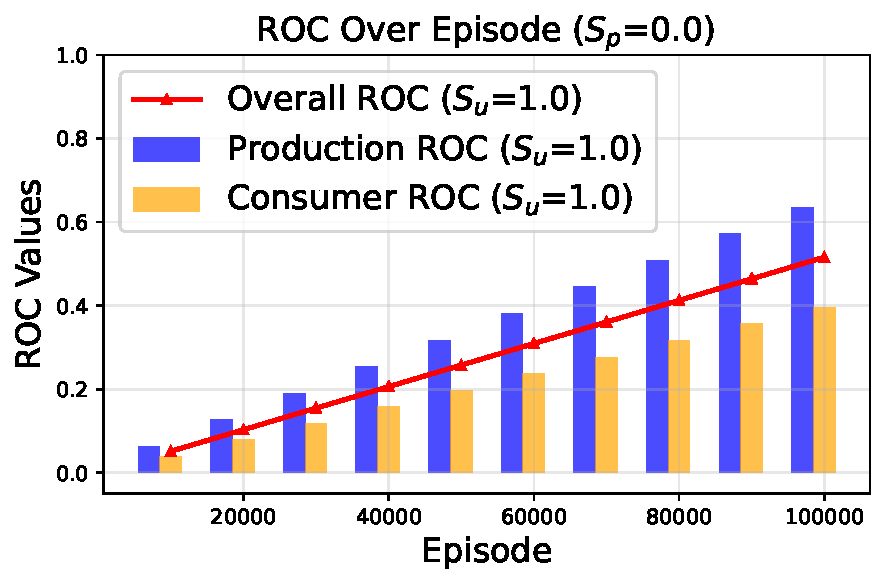
\includegraphics[width=\linewidth]{figures/fixed_sp/population_strategy_0_0_roc.pdf}
        % \caption{0}
    \end{subfigure}
    % \hfill
    \begin{subfigure}[b]{0.162\linewidth}
        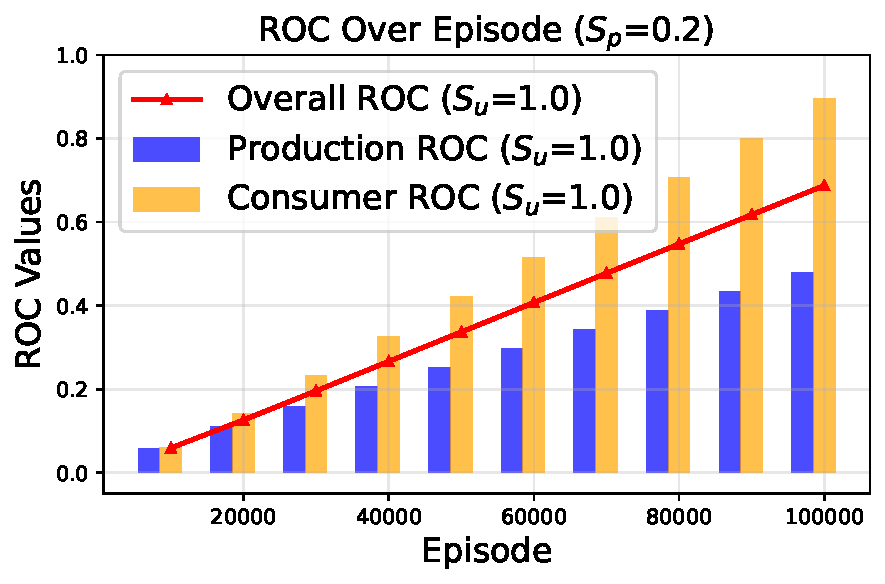
\includegraphics[width=\linewidth]{figures/fixed_sp/population_strategy_0_2_roc.pdf}
        % \caption{0.2}
    \end{subfigure}
    % \hfill
    \begin{subfigure}[b]{0.162\linewidth}
        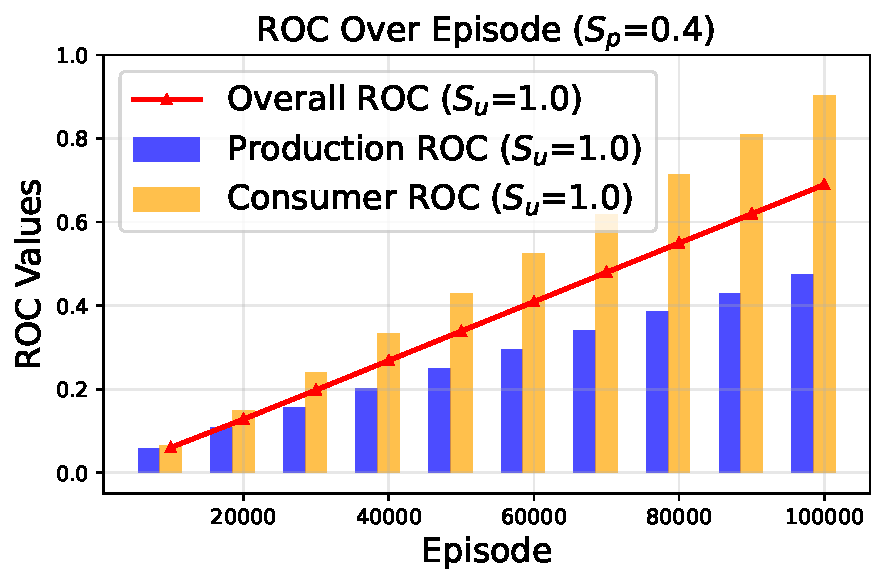
\includegraphics[width=\linewidth]{figures/fixed_sp/population_strategy_0_4_roc.pdf}
        % \caption{0.4}
    \end{subfigure}
    % \hfill
    \begin{subfigure}[b]{0.162\linewidth}
        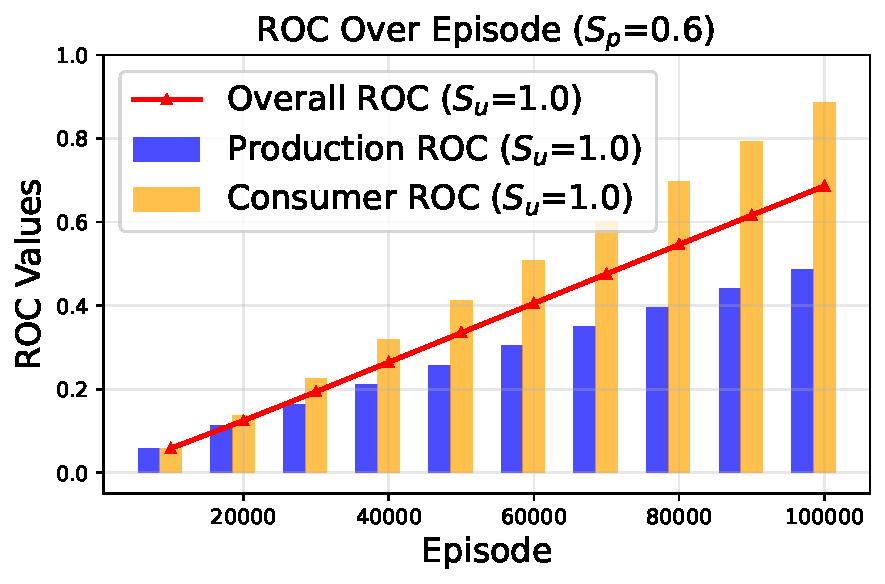
\includegraphics[width=\linewidth]{figures/fixed_sp/population_strategy_0_6_roc.pdf}
        % \caption{0.6}
    \end{subfigure}
    % \hfill
    \begin{subfigure}[b]{0.162\linewidth}
        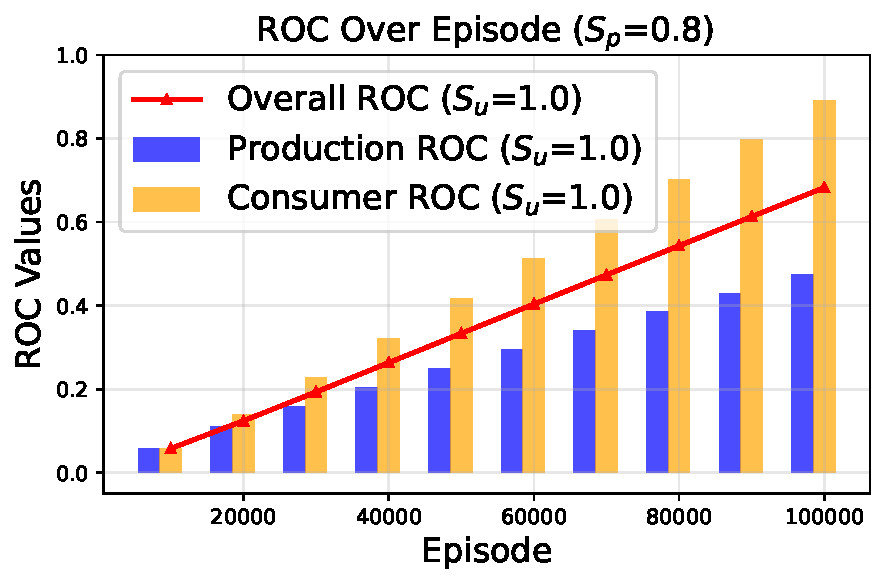
\includegraphics[width=\linewidth]{figures/fixed_sp/population_strategy_0_8_roc.pdf}
        % \caption{0.8}
    \end{subfigure}
    % \hfill
    \begin{subfigure}[b]{0.162\linewidth}
        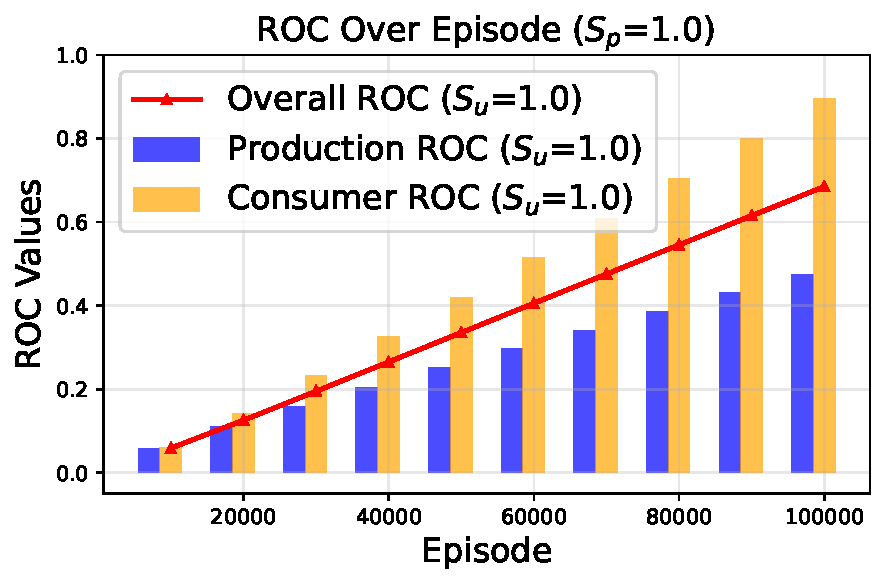
\includegraphics[width=\linewidth]{figures/fixed_sp/population_strategy_1_0_roc.pdf}
        % \caption{1.0}
    \end{subfigure}
    \vspace{1mm}
    \begin{subfigure}[b]{0.162\linewidth}
        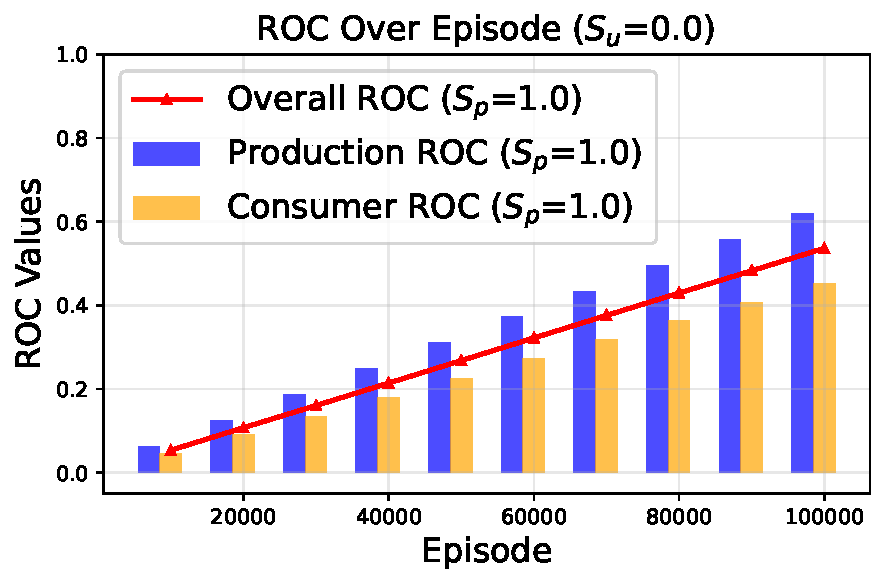
\includegraphics[width=\linewidth]{figures/fixed_su/user_strategy_0_0_roc.pdf}
        % \caption{0}
    \end{subfigure}
    % \hfill
    \begin{subfigure}[b]{0.162\linewidth}
        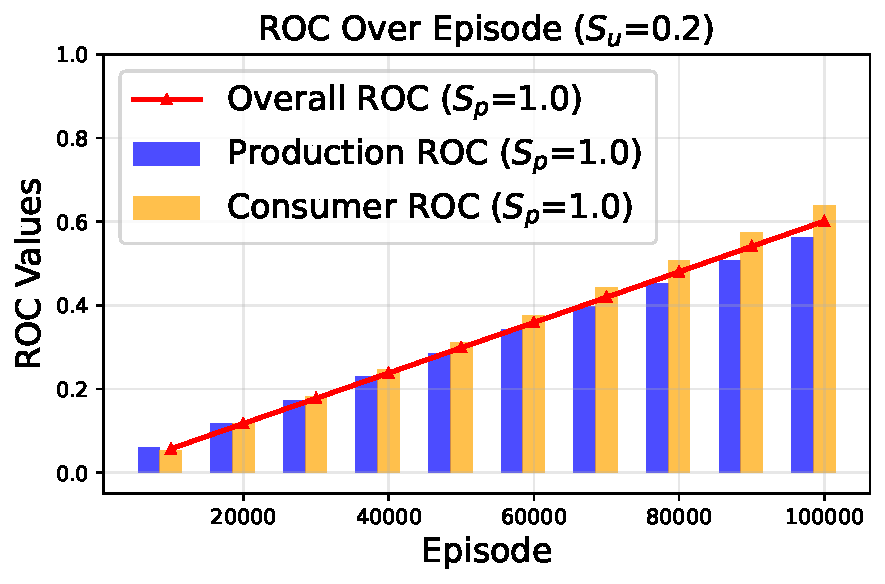
\includegraphics[width=\linewidth]{figures/fixed_su/user_strategy_0_2_roc.pdf}
        % \caption{0.2}
    \end{subfigure}
    % \hfill
    \begin{subfigure}[b]{0.162\linewidth}
        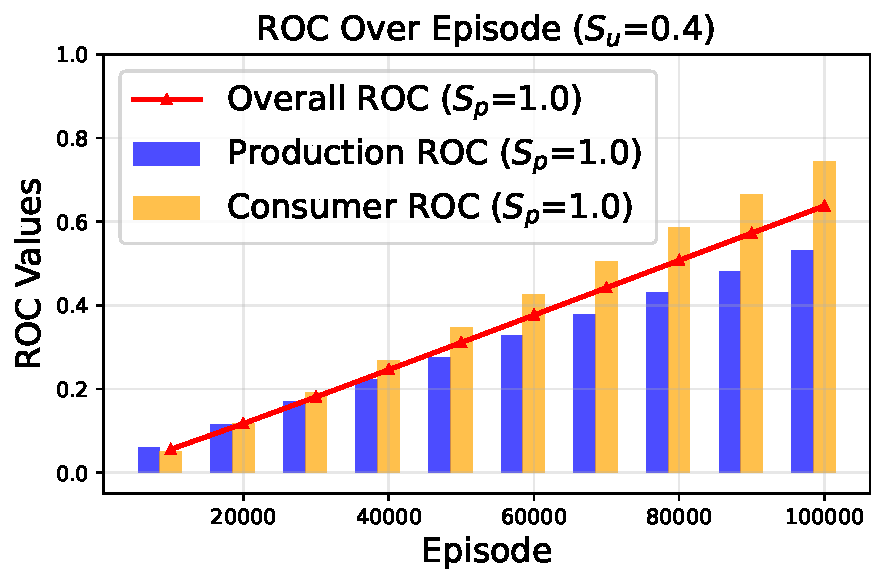
\includegraphics[width=\linewidth]{figures/fixed_su/user_strategy_0_4_roc.pdf}
        % \caption{0.4}
    \end{subfigure}
    % \hfill
    \begin{subfigure}[b]{0.162\linewidth}
        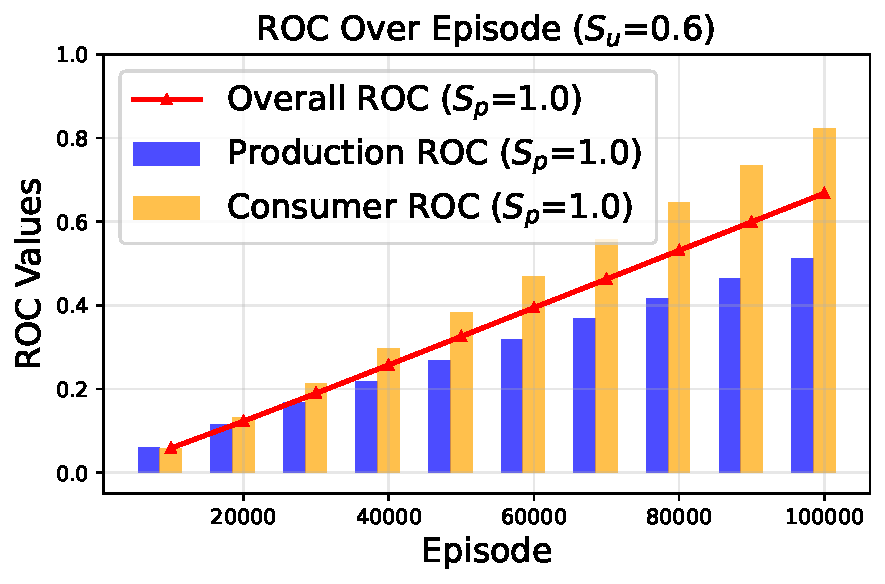
\includegraphics[width=\linewidth]{figures/fixed_su/user_strategy_0_6_roc.pdf}
        % \caption{0.6}
    \end{subfigure}
    % \hfill
    \begin{subfigure}[b]{0.162\linewidth}
        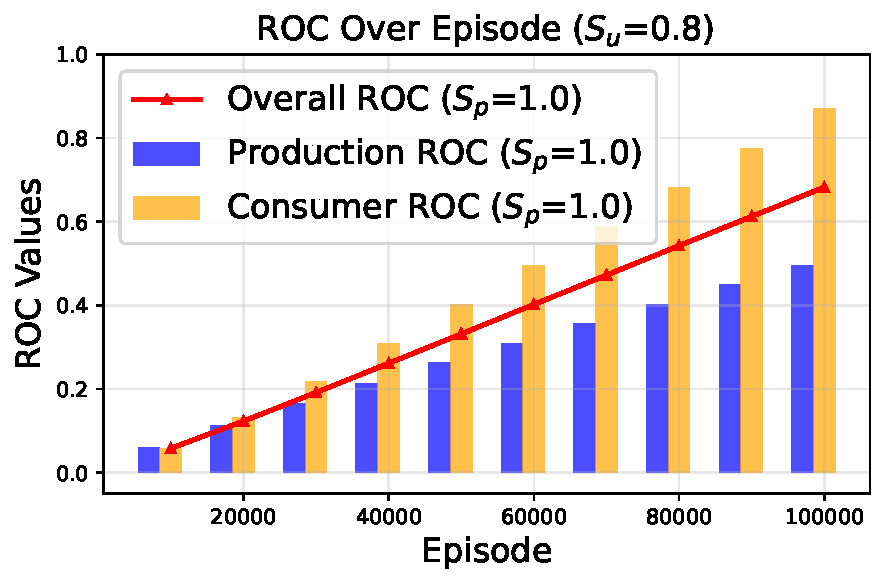
\includegraphics[width=\linewidth]{figures/fixed_su/user_strategy_0_8_roc.pdf}
        % \caption{0.8}
    \end{subfigure}
    % \hfill
    \begin{subfigure}[b]{0.162\linewidth}
        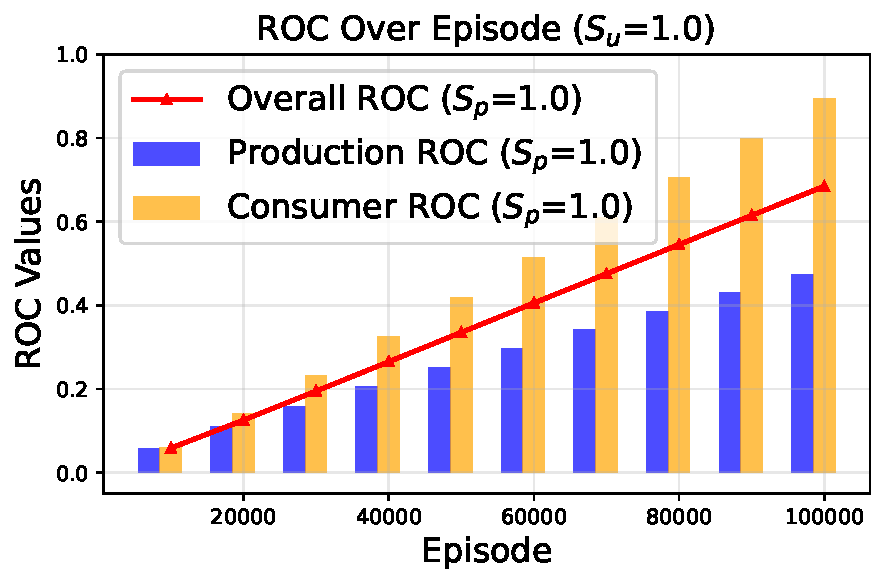
\includegraphics[width=\linewidth]{figures/fixed_su/user_strategy_1_0_roc.pdf}
        % \caption{1.0}
    \end{subfigure}
    \vspace{-4mm}
    \caption{ROC comparison over 100,000 episode based on different strategy. }
    \label{ROC Comp}
    \vspace{-1mm}
\end{figure*}

\begin{figure*}[t]
    \centering
    \begin{subfigure}[b]{0.162\linewidth}
        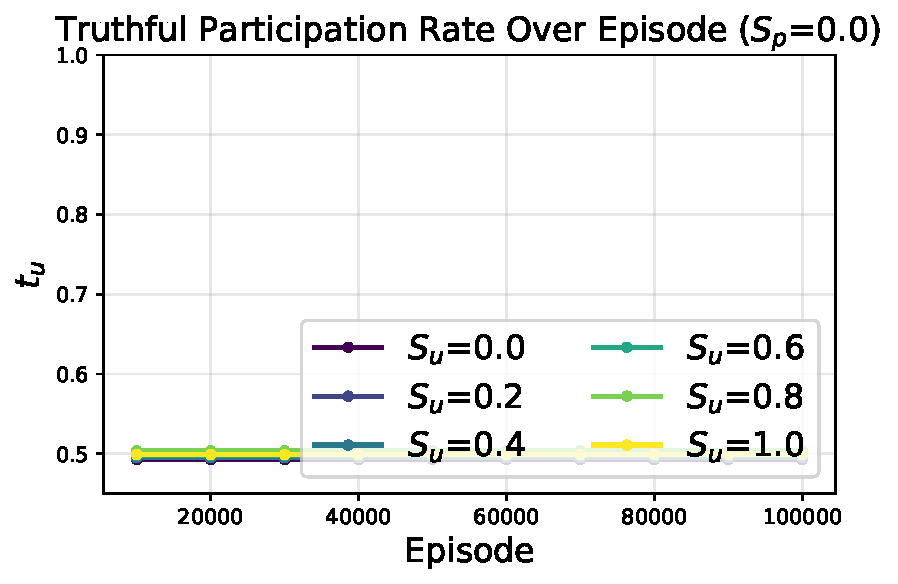
\includegraphics[width=\linewidth]{figures/fixed_sp/population_strategy_0_0_hard.pdf}
        % \caption{0}
    \end{subfigure}
    % \hfill
    \begin{subfigure}[b]{0.162\linewidth}
        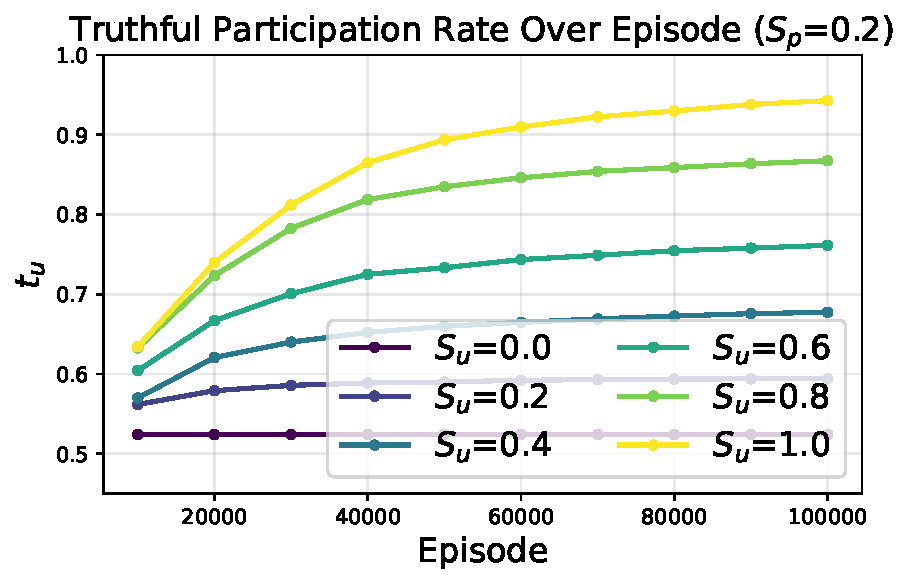
\includegraphics[width=\linewidth]{figures/fixed_sp/population_strategy_0_2_hard.pdf}
        % \caption{0.2}
    \end{subfigure}
    % \hfill
    \begin{subfigure}[b]{0.162\linewidth}
        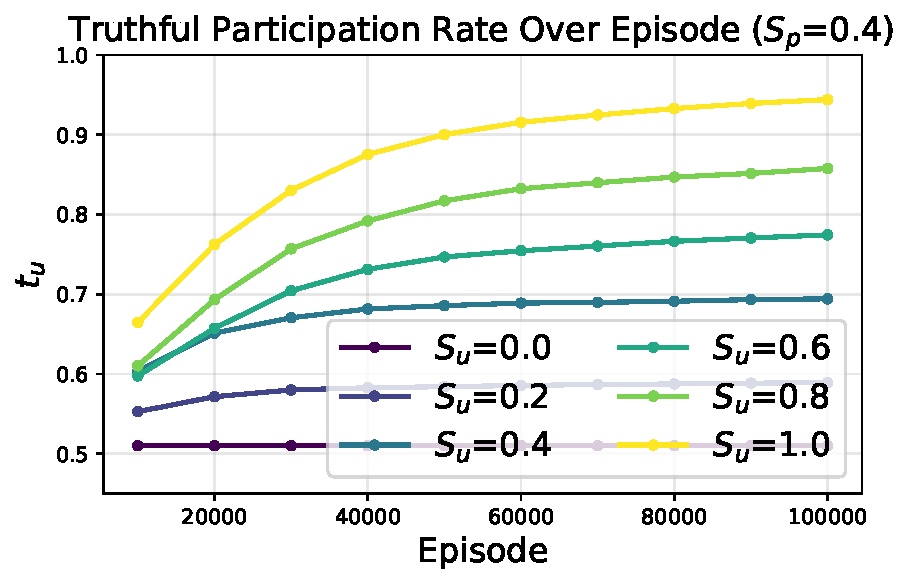
\includegraphics[width=\linewidth]{figures/fixed_sp/population_strategy_0_4_hard.pdf}
        % \caption{0.4}
    \end{subfigure}
    % \hfill
    \begin{subfigure}[b]{0.162\linewidth}
        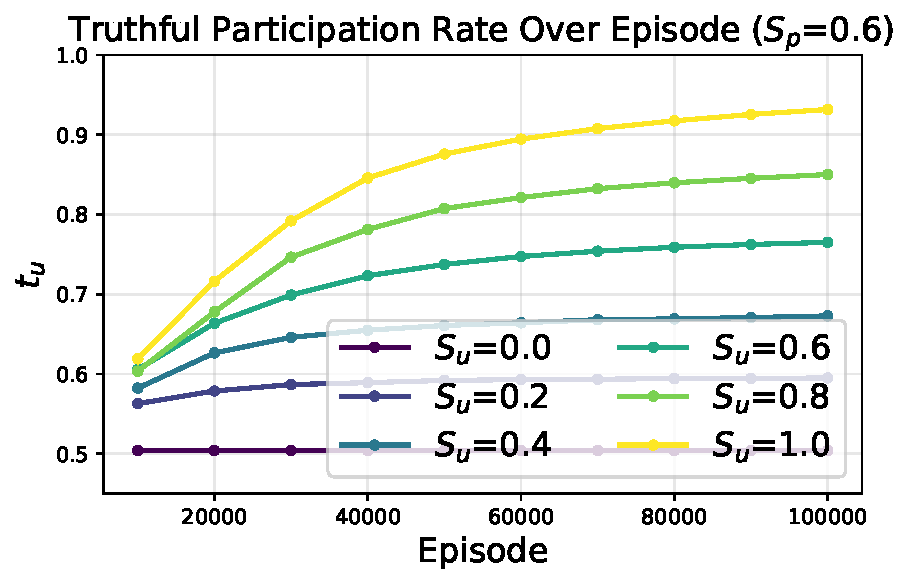
\includegraphics[width=\linewidth]{figures/fixed_sp/population_strategy_0_6_hard.pdf}
        % \caption{0.6}
    \end{subfigure}
    % \hfill
    \begin{subfigure}[b]{0.162\linewidth}
        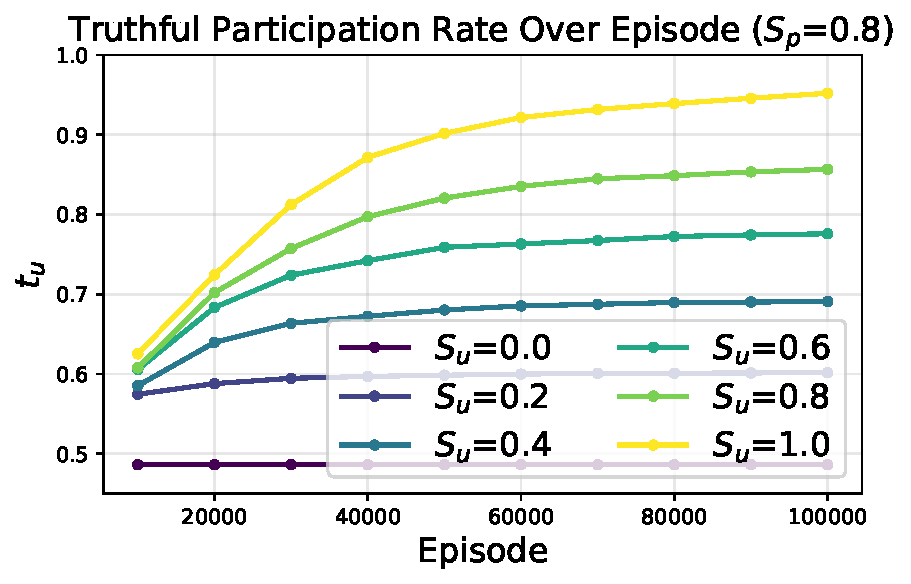
\includegraphics[width=\linewidth]{figures/fixed_sp/population_strategy_0_8_hard.pdf}
        % \caption{0.8}
    \end{subfigure}
    % \hfill
    \begin{subfigure}[b]{0.162\linewidth}
        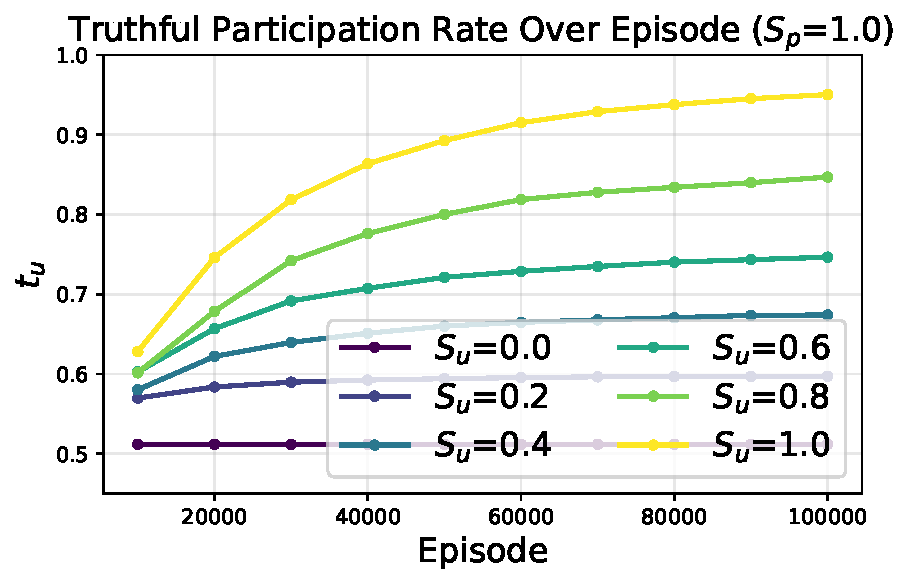
\includegraphics[width=\linewidth]{figures/fixed_sp/population_strategy_1_0_hard.pdf}
        % \caption{1.0}
    \end{subfigure}

    \vspace{1mm}

    \begin{subfigure}[b]{0.162\linewidth}
        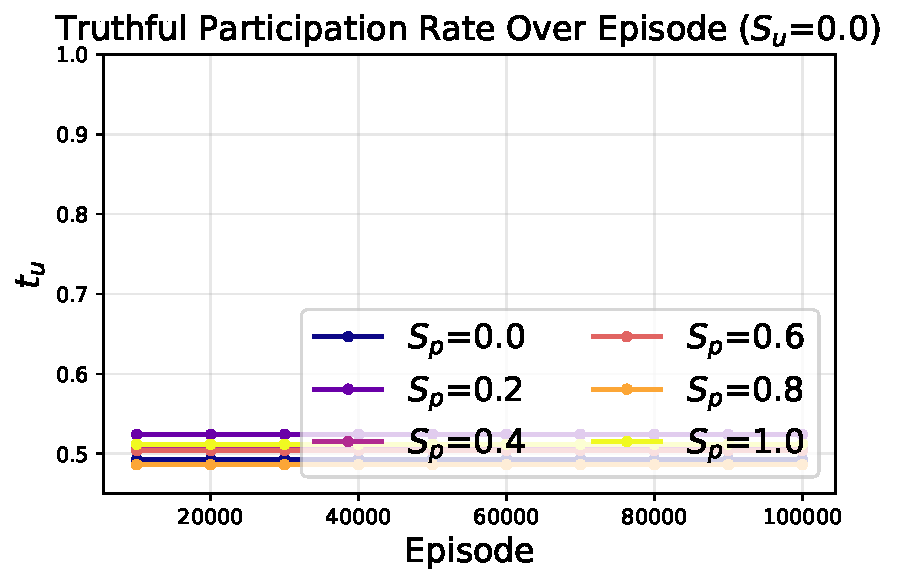
\includegraphics[width=\linewidth]{figures/fixed_su/user_strategy_0_0_hard.pdf}
        % \caption{0}
    \end{subfigure}
    % \hfill
    \begin{subfigure}[b]{0.162\linewidth}
        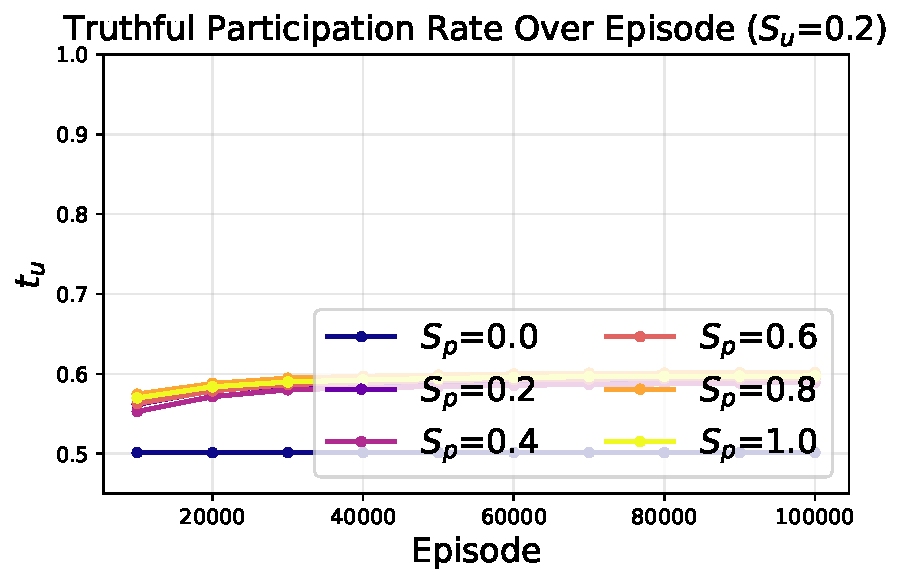
\includegraphics[width=\linewidth]{figures/fixed_su/user_strategy_0_2_hard.pdf}
        % \caption{0.2}
    \end{subfigure}
    % \hfill
    \begin{subfigure}[b]{0.162\linewidth}
        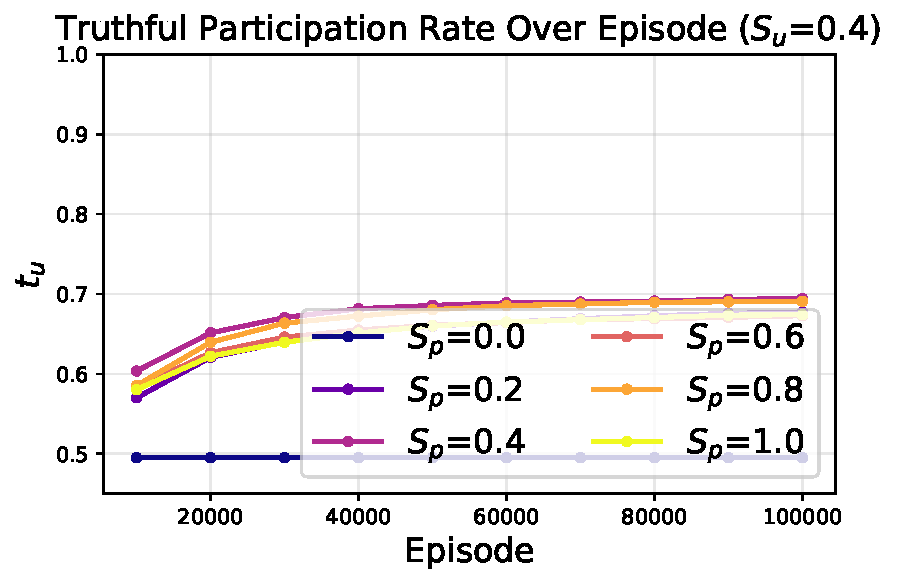
\includegraphics[width=\linewidth]{figures/fixed_su/user_strategy_0_4_hard.pdf}
        % \caption{0.4}
    \end{subfigure}
    % \hfill
    \begin{subfigure}[b]{0.162\linewidth}
        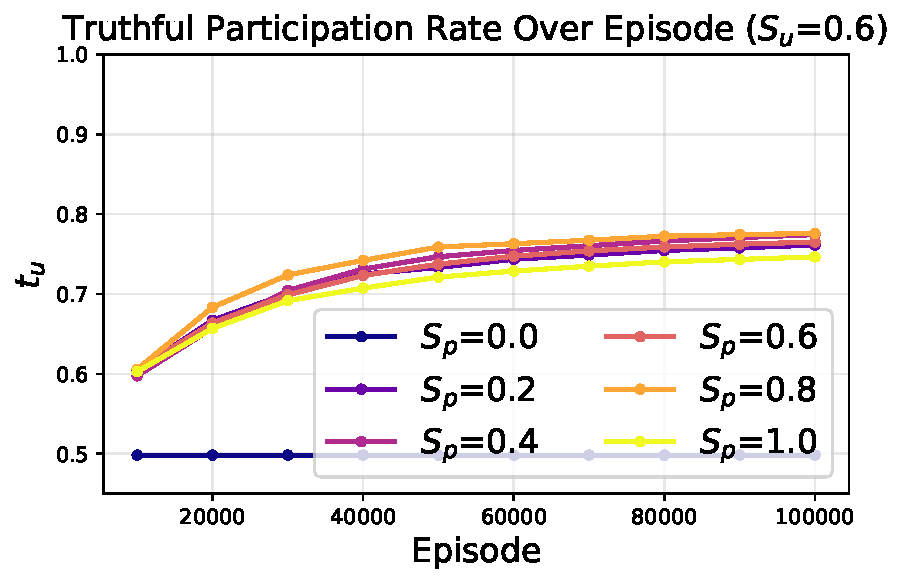
\includegraphics[width=\linewidth]{figures/fixed_su/user_strategy_0_6_hard.pdf}
        % \caption{0.6}
    \end{subfigure}
    % \hfill
    \begin{subfigure}[b]{0.162\linewidth}
        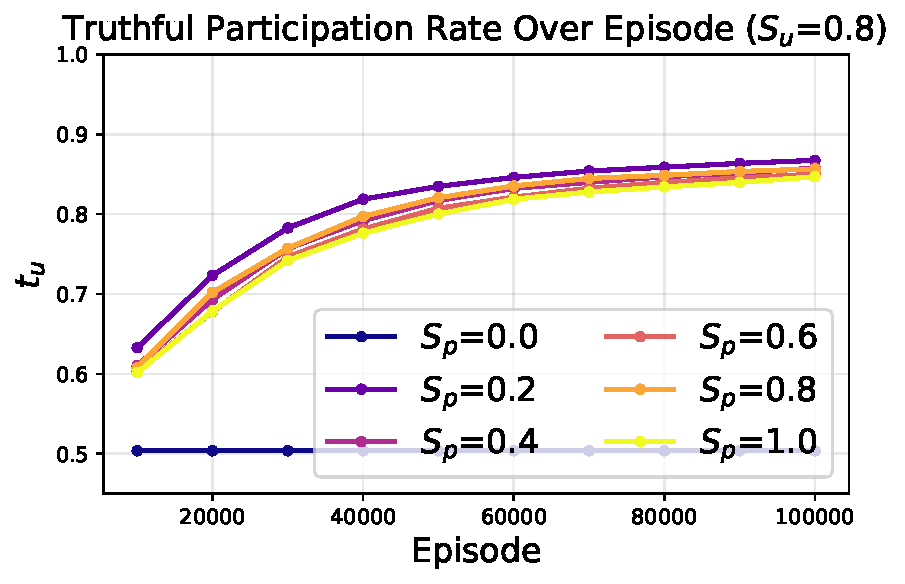
\includegraphics[width=\linewidth]{figures/fixed_su/user_strategy_0_8_hard.pdf}
        % \caption{0.8}
    \end{subfigure}
    % \hfill
    \begin{subfigure}[b]{0.162\linewidth}
        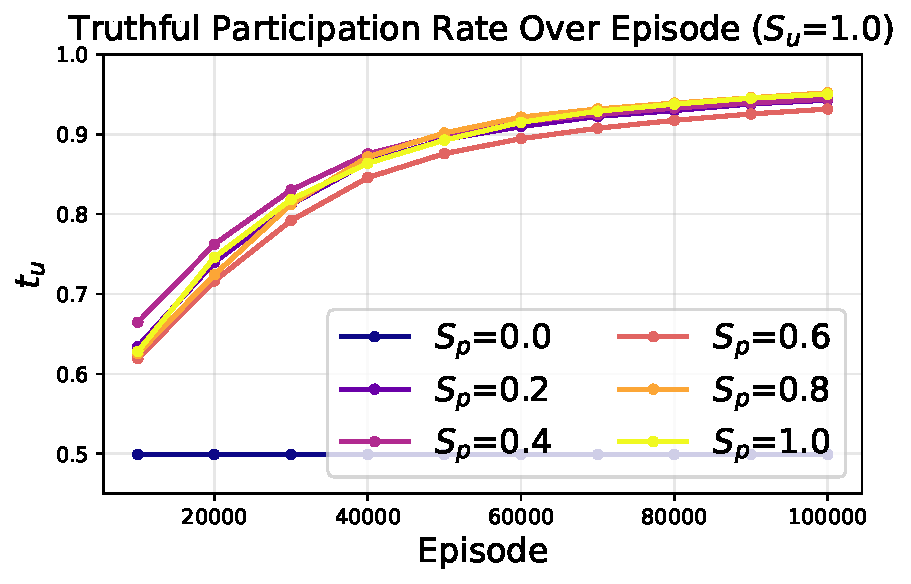
\includegraphics[width=\linewidth]{figures/fixed_su/user_strategy_1_0_hard.pdf}
        % \caption{1.0}
    \end{subfigure}
    \vspace{-3mm}
    \caption{Truthful participation comparison with different $S_{u}$ and $S_{p}$.}
        \label{Truthful participation comparison}
\end{figure*}
\vspace{-4mm}


\section{Theoretical Foundations and Empirical Validation}

This section provides the game-theoretic underpinning of the ecosystem designed in \Cref{sec:ecosystem} and empirically validates the framework through a case study.
We first formalize the Bayesian validation game, establish assumptions, and derive incentive compatibility for validators (\S\ref{sec:ic}).
We then characterize threshold-optimal policies for producers (\S\ref{sec:producer_ir}) and consumers (\S\ref{sec:consumer_ir}), prove the existence of a symmetric Bayesian--Nash equilibrium (\S\ref{sec:bne}), and analyze the resulting tokenomics--knowledge dual loop.
Finally, we instantiate the ecosystem as a decentralized question answering system and present simulation results (\S\ref{sec:case_study}).

\subsection{Game-Theoretic Guarantees}
\label{sec:game_theory}

\subsubsection{Model Setup and Assumptions}

We model the ecosystem as a Bayesian game among three types of strategic agents---validators, producers, and consumers---interacting through the mechanism described in \Cref{sec:ecosystem}.

\vspace{1mm}
\noindent\textbf{Game Structure.}
The game proceeds in four stages for each service engagement:
\begin{enumerate}[leftmargin=2em]
    \item \textbf{Nature's move}: Each agent $u \in \mathcal{U}$ is endowed with a private quality type $q_u \in (\frac{1}{2}, 1]$, drawn independently from a common prior distribution $F$ over $(\frac{1}{2}, 1]$. The quality $q_u$ is private information known only to $u$.
    \item \textbf{Validation stage}: The requester (producer or consumer) selects $n$ validators and presents $m$ sample tasks. Each validator $v_i$ chooses an effort level $e_i \in \{0, 1\}$ (shirk or exert effort), then submits a report. Reports are aggregated by majority vote to produce a consensus signal $Z \in \{0, 1\}$.
    \item \textbf{Decision stage}: The requester observes $Z$ and decides whether to proceed (promote or subscribe).
    \item \textbf{Payoff realization}: Tokens are transferred according to the mechanism rules described in \Cref{sec:ecosystem}, and validators' stakes are distributed based on their agreement with the consensus.
\end{enumerate}

\noindent\textbf{Strategy Spaces.}
Each validator's strategy is a mapping from its type $q_v$ to an effort choice $e \in \{0, 1\}$.
Each producer's strategy is a mapping from its type $q_p$ to a promotion decision $d_p \in \{0, 1\}$.
Each consumer's strategy is a mapping from its type and the observed consensus $Z$ to a subscription decision $d_c \in \{0, 1\}$.
A \textit{symmetric} strategy profile requires that all agents of the same role use the same strategy mapping.

\vspace{1mm}
\noindent\textbf{Assumptions.}
We now formalize the assumptions that underpin all subsequent results.

\begin{assumption}[Validator Population and Independence]
\label{assum:validators}
The validation committee consists of $n$ validators (where $n$ is odd to avoid ties), each possessing individual service quality $q_v > \frac{1}{2}$. Validators are drawn independently from the agent population and make decisions independently (no collusion). This independence assumption is operationalized at the protocol level through the \textit{architectural heterogeneity requirement} described in \Cref{sec:ecosystem}, which mandates that validators employ model architectures distinct from the producer and from each other. While architectural diversity cannot eliminate all residual correlation (e.g., from overlapping training corpora), it removes the dominant source of correlated failures---shared model weights and decoding procedures---making approximate independence a defensible modeling choice (see Limitations in \Cref{sec:conclusion} for further discussion).
\end{assumption}

\begin{assumption}[Binary Signal Model]
\label{assum:binary}
For each sample task $x_j$ in the task set, each validator $v_i$ independently produces a per-task binary judgment: $r_{ij} = 1$ (producer's output is correct) or $r_{ij} = 0$ (incorrect). Under truthful effort, $\Pr(r_{ij} = \text{truth}) = q_v$; under shirking (zero effort), $\Pr(r_{ij} = 1) = \frac{1}{2}$ (random guess). Validator $v_i$'s aggregate judgment across the $m$ sample tasks is determined by majority vote over its per-task judgments:
\[
r_i = \mathbbm{1}\!\left[\sum_{j=1}^{m} r_{ij} > \tfrac{m}{2}\right],
\]
so $r_i = 1$ (agree) iff the producer's outputs are correct on a strict majority of sample tasks according to $v_i$'s assessment.
\end{assumption}

\begin{assumption}[Cost Structure]
\label{assum:costs}
Producing a truthful judgment on one task costs $c_u > 0$ (computation, knowledge retrieval). Shirking costs zero. The validation fee satisfies $\tau_{\text{val}} > c_u$ (honest effort is individually viable), and the total validation cost satisfies $mn\tau_{\text{val}} \ll \tau_p \ll \tau_s$ (validation is cheap relative to promotion and subscription).
\end{assumption}

\begin{assumption}[Monotone Likelihood Ratio Property (MLRP)]
\label{assum:mlrp}
The probability that a producer passes majority-vote validation is strictly increasing in its true quality $q_p$. Formally, for the consensus signal $Z \in \{0, 1\}$ (pass/fail), the pass probability $V(q_p) \coloneqq \Pr(Z = 1 \mid q_p)$ is a strictly increasing, continuous function of $q_p$.
\end{assumption}

\begin{remark}[MLRP as a Consequence]
\label{rem:mlrp_derived}
Assumption~\ref{assum:mlrp} is not an independent postulate but follows from Assumptions~\ref{assum:validators}--\ref{assum:costs}: the per-task agreement probability $p_{\text{agree}}(q_p, q_v) = q_p q_v + (1 - q_p)(1 - q_v)$ is strictly increasing in $q_p$ for $q_v > \frac{1}{2}$, and this monotonicity propagates through majority voting to $V(q_p)$. See Appendix~\ref{app:mlrp_derived} for details.
\end{remark}

\noindent\textbf{Extension to $m$ queries.}
Since tasks are i.i.d., the IC condition scales linearly and simplifies to the same per-task condition. We derive all results for $m = 1$ without loss of generality (see Appendix~\ref{app:m_extension}).

\vspace{1mm}
Under these assumptions, we now derive the three layers of incentive guarantees.


\subsubsection{Incentive Compatibility (IC) of Validators}
\label{sec:ic}

The first and most fundamental question is whether the validation mechanism can be trusted at all.
If validators shirk---submitting random judgments to avoid effort costs---then the consensus signal $Z$ carries no information, and the entire ecosystem collapses: producers cannot credibly signal quality, consumers cannot make informed subscription decisions, and the tokenomics--knowledge dual loop breaks down.
We therefore begin by analyzing the validator's decision problem and deriving the conditions under which truthful effort is each validator's strict best response.

Consider a single validator $v_i$ who must choose between exerting truthful effort ($e = 1$) and free-riding ($e = 0$), taking as given that the other $n - 1$ validators play truthfully.
This is a standard Bayesian incentive analysis: we compute the expected payoff under each strategy and identify when truthful effort strictly dominates.

\vspace{1mm}
\noindent\textbf{Payoff Structure.}
Recall from \Cref{sec:ecosystem} that each validator stakes $\sigma$ and receives a reward if its report matches the majority.
We adopt a conservative lower bound on the per-capita reward: if $k$ out of $n$ validators agree with the majority, the total reward pool of $m n \tau_{\text{val}} + n\sigma$ (requester payments plus all stakes) is split among them. In the worst case where all $n$ validators agree, each receives:
\begin{equation}
R_{\min} = \frac{mn\tau_{\text{val}} + n\sigma}{n} = m\tau_{\text{val}} + \sigma.
\end{equation}
For one sample (the per-query case $m = 1$ that we analyze without loss of generality, since tasks are i.i.d.), we have $R_{\min} = \tau_{\text{val}} + \sigma$.
A validator who disagrees with the majority forfeits $\sigma$ and receives nothing.

\vspace{1mm}
\noindent\textbf{Matching Probability under Truthful Play.}
Let $P_{\text{match}}(n, q_v)$ denote the probability that a truthful validator's vote matches the majority when all $n$ validators report truthfully. By conditioning on whether $v_i$'s report is correct (probability $q_v$) or incorrect (probability $1 - q_v$), and computing the probability that a majority of the remaining $n-1$ validators agree in each case, we obtain (see Appendix~\ref{app:pmatch_derivation} for the full derivation):
\begin{equation}
\label{eq:pmatch}
P_{\text{match}}(n, q_v) = q_v \cdot \alpha(n, q_v) + (1 - q_v) \cdot \beta(n, q_v),
\end{equation}
where $\alpha$ and $\beta$ are binomial tail probabilities with parameters $q_v$ and $1-q_v$ respectively.

\begin{proposition}[Properties of $P_{\text{match}}$]
\label{prop:pmatch_properties}
The matching probability satisfies:
\textbf{(i)}~$P_{\text{match}}(n, q_v) > \frac{1}{2}$ for all $q_v > \frac{1}{2}$ (by the Condorcet jury theorem);
\textbf{(ii)}~$P_{\text{match}}$ is strictly increasing in both $q_v$ and $n$;
\textbf{(iii)}~$P_{\text{match}} \to 1$ as $n \to \infty$.
\end{proposition}
\noindent\textit{Proof.} See Appendix~\ref{app:pmatch_properties}. The key insight for (i) is that $P_{\text{match}} \geq q_v^2 + (1-q_v)^2 > \frac{1}{2}$. \qed

\vspace{1mm}
\noindent\textbf{Expected Payoffs.}
Given the payoff structure and matching probability, the expected utilities under the two strategies are:

Under \textbf{truthful effort} ($e = 1$): the validator matches the majority with probability $P_{\text{match}}$, earning $R_{\min}$, and fails to match with probability $1 - P_{\text{match}}$, losing $\sigma$. The effort costs $c_u$:
\begin{equation}
\label{eq:u_truthful}
\mathbb{E}[U \mid e = 1] = P_{\text{match}} \cdot R_{\min} - (1 - P_{\text{match}}) \cdot \sigma - c_u.
\end{equation}

Under \textbf{free-riding} ($e = 0$): the validator submits a random vote, which matches any majority with probability exactly $\frac{1}{2}$ (since a uniform random vote is independent of the majority outcome; see Appendix~\ref{app:freeriding}). Therefore:
\begin{equation}
\label{eq:u_shirk}
\mathbb{E}[U \mid e = 0] = \frac{1}{2} \cdot R_{\min} - \frac{1}{2} \cdot \sigma = \frac{1}{2}(R_{\min} - \sigma).
\end{equation}

\begin{theorem}[IC Condition for Validators]
\label{Strict IC for Validators}
Under Assumptions~\ref{assum:validators}--\ref{assum:costs}, truthful effort is a strict best response for each validator if and only if:
\begin{equation}
\label{eq:ic}
(\tau_{\text{val}} + 2\sigma)\Big(P_{\text{match}}(n, q_v) - \frac{1}{2}\Big) > c_u.
\end{equation}
\end{theorem}

\begin{proof}[Proof sketch (full proof in Appendix~\ref{app:proof_ic})]
Requiring $\mathbb{E}[U \mid e=1] > \mathbb{E}[U \mid e=0]$ and substituting Equations~\eqref{eq:u_truthful}--\eqref{eq:u_shirk}, the algebra reduces to $(R_{\min} + \sigma)(P_{\text{match}} - \frac{1}{2}) > c_u$. The IC condition decomposes into a product of the \textit{total economic stake} $(R_{\min} + \sigma) = \tau_{\text{val}} + 2\sigma$ and the \textit{informational edge} $(P_{\text{match}} - \frac{1}{2})$ that truthful effort provides over random guessing.
\end{proof}

\begin{interpretbox}{Takeaway: Economic Interpretation of Validator IC}
The IC condition $(\tau_{\text{val}} + 2\sigma)(P_{\text{match}} - \frac{1}{2}) > c_u$ decomposes into three interpretable components:
\begin{itemize}[leftmargin=1.5em, itemsep=2pt]
    \item $(\tau_{\text{val}} + 2\sigma)$: \textbf{Total economic exposure}---the validation fee plus twice the stake, capturing the amount ``at risk'' that amplifies the value of being on the right side of consensus.
    \item $(P_{\text{match}} - \frac{1}{2})$: \textbf{Informational advantage}---how much better a truthful vote aligns with the majority compared to a random coin flip. Larger committees and higher-quality validators widen this gap.
    \item $c_u$: \textbf{Effort cost}---the computational expense that must be overcome. IC holds when the marginal benefit of being informed exceeds the cost of becoming informed.
\end{itemize}
\end{interpretbox}

\noindent\textbf{Comparative Statics.}
The IC region---the set of parameters for which~\eqref{eq:ic} holds---expands when:
\begin{enumerate}[leftmargin=2em]
    \item $\tau_{\text{val}}$ or $\sigma$ increases: higher economic exposure amplifies the cost of being wrong.
    \item $q_v$ increases: more capable validators have a larger informational advantage.
    \item $n$ increases: larger committees strengthen the majority, raising $P_{\text{match}}$.
    \item $c_u$ decreases: cheaper effort is easier to incentivize.
\end{enumerate}
In the limit $n \to \infty$, $P_{\text{match}} \to 1$, so IC holds for any finite $c_u$ given sufficient economic exposure. In practice, a moderate committee size $n \in \{5, 9, 17\}$ is sufficient when $q_v$ is reasonably above $\frac{1}{2}$.


\subsubsection{Producer's Threshold-Optimal Promotion}
\label{sec:producer_ir}

Having established that validators can be trusted to report truthfully (Theorem~\ref{Strict IC for Validators}), we now ask the next logical question in the mechanism's causal chain: \textit{given that the consensus signal $Z$ is informative, when should a producer rationally choose to promote its service?}
This is the supply-side participation problem.
If no producer is willing to pay the promotion fee and face validation, the ecosystem has no services to offer---regardless of how well the validation layer works.

The question is non-trivial because promotion involves upfront costs (the promotion fee $\tau_p$ and validation costs $mn\tau_{\text{val}}$) against an uncertain prospect of subscription revenue.

\vspace{1mm}
\noindent\textbf{Setup.}
A producer with true quality $q_p$ considers promoting its service $a_p$. If it proceeds, it pays:
\begin{itemize}
    \item Promotion fee: $\tau_p$
    \item Validation cost: $mn\tau_{\text{val}}$ (paying $n$ validators for $m$ sample tasks)
\end{itemize}
Majority voting among validators generates a public consensus signal $Z \in \{0, 1\}$ (pass/fail). Under Assumption~\ref{assum:mlrp}, the pass probability $V_p(q_p) = \Pr(Z = 1 \mid q_p)$ is strictly increasing in $q_p$.

If the producer passes validation ($Z = 1$) and the consumer subsequently subscribes, the producer receives subscription revenue $\tau_s$ but incurs future service costs $c_s > 0$ (the net present value of all future service obligations). The net surplus from a successful subscription is therefore $\tau_s - c_s$.

\vspace{1mm}
\noindent\textbf{Expected Payoff.}
The producer's expected payoff from promotion is:
\begin{equation}
\label{eq:producer_payoff}
\Pi_p(q_p) = V_p(q_p) \cdot (\tau_s - c_s) - (\tau_p + mn\tau_{\text{val}}).
\end{equation}
The first term is the expected subscription surplus (pass probability times net revenue); the second is the certain upfront cost.

\begin{theorem}[IR-based Policy for Producers]
\label{IR for Producers}
Under Assumption~\ref{assum:mlrp}, there exists a unique quality threshold $\bar{q}_p \in (0, 1)$ such that promotion is the producer's best response if and only if:
\begin{equation}
\label{eq:producer_threshold}
V_p(q_p) \cdot (\tau_s - c_s) \geq \tau_p + mn\tau_{\text{val}} \quad \Longleftrightarrow \quad q_p \geq \bar{q}_p.
\end{equation}
\end{theorem}

\begin{proof}[Proof sketch (full proof in Appendix~\ref{app:proof_producer_ir})]
Since $V_p(q_p) \cdot (\tau_s - c_s)$ is strictly increasing and continuous in $q_p$ (by Assumption~\ref{assum:mlrp}), is negative at $q_p = \frac{1}{2}$ and positive at $q_p = 1$ (by the cost ordering $mn\tau_{\text{val}} \ll \tau_p \ll \tau_s$), the intermediate value theorem yields a unique crossing point $\bar{q}_p$.
\end{proof}

\begin{interpretbox}{Takeaway: Supply-Side Self-Screening}
The threshold $\bar{q}_p$ implements self-screening without centralized curation. Producers below $\bar{q}_p$ know they are likely to fail validation, making promotion unprofitable---they rationally abstain. Producers above $\bar{q}_p$ expect to pass and earn subscription revenue---they rationally promote. The market thus \textit{self-selects} for quality: the very act of paying promotion and validation fees serves as a credible signal of competence, because only agents who expect to pass can afford the risk.
\end{interpretbox}

\noindent\textbf{Comparative Statics.}
The threshold $\bar{q}_p$ responds to mechanism parameters as follows:
\begin{itemize}
    \item Higher $\tau_p$ or $\tau_{\text{val}}$ $\Rightarrow$ higher $\bar{q}_p$: more expensive entry screens more stringently.
    \item Higher $\tau_s$ $\Rightarrow$ lower $\bar{q}_p$: larger subscription revenue attracts more producers.
    \item Larger $m$ or $n$ (more informative validation) $\Rightarrow$ steeper $V_p$ $\Rightarrow$ lower $\bar{q}_p$: better validation allows lower-quality producers to be reliably filtered, so the threshold can be relaxed.
\end{itemize}


\subsubsection{Consumer's Threshold-Optimal Subscription}
\label{sec:consumer_ir}

The analysis so far has established two layers of the mechanism: validators truthfully report (IC), and producers self-screen by promoting only when sufficiently capable (IR). The final piece is the demand side: \textit{given that the consensus $Z$ is informative and that only competent producers enter the market, when should a consumer rationally commit tokens to a subscription?}

This completes the causal chain of the mechanism. The consumer's problem differs from the producer's in a fundamental way: while the producer knows its own quality $q_p$ and decides whether to enter, the consumer does \textit{not} know $q_p$ and must \textit{infer} it from the noisy consensus signal $Z$. This makes the consumer's problem inherently Bayesian---it must form a posterior belief about producer quality and subscribe only when the expected posterior utility justifies the cost.

\vspace{1mm}
\noindent\textbf{Setup.}
The consumer pays subscription fee $\tau_s$ and validation cost $mn\tau_{\text{val}}$ (for the subscription-stage validation). Majority voting produces a consensus signal $Z \in \{0, 1\}$.

Let $V_c(q_p)$ denote the consumer's \textit{per-subscription value function}---the discounted expected utility from delegating future tasks to a producer of quality $q_p$. The only property required for our analysis is that $V_c(\cdot)$ is \textit{strictly increasing and continuous} in $q_p$ (higher producer quality yields higher consumer utility). A concrete parametric form---$V_c(q_p) = \frac{1-\delta^T}{1-\delta}[q_p \cdot b - (1-q_p) \cdot \ell]$ for discount factor $\delta$, horizon $T$, benefit $b > 0$, and loss $\ell \geq 0$---is provided in Appendix~\ref{app:proof_consumer_ir}, but the results hold for any monotone $V_c$.

\vspace{1mm}
\noindent\textbf{Posterior Utility under Validation.}
The consumer does not directly observe $q_p$ but instead observes the consensus signal $Z$.
Using Bayes' rule, the consumer forms a posterior belief over $q_p$ conditional on $Z$:
\begin{equation}
\label{eq:posterior}
f(q_p \mid Z = 1) = \frac{\Pr(Z = 1 \mid q_p) \cdot f(q_p)}{\Pr(Z = 1)} = \frac{V(q_p) \cdot f(q_p)}{\int V(q) f(q) \, dq},
\end{equation}
where $f(\cdot)$ is the prior density over producer quality (from Nature's move).
The posterior expected utility from subscribing, conditional on a ``pass'' signal, is:
\begin{equation}
\label{eq:consumer_posterior}
\mathbb{E}[V_c(q_p) \mid Z = 1] = \int V_c(q_p) \cdot f(q_p \mid Z = 1) \, dq_p.
\end{equation}

Since $V(q_p) = \Pr(Z = 1 \mid q_p)$ is strictly increasing in $q_p$ (Assumption~\ref{assum:mlrp}), the posterior $f(q_p \mid Z = 1)$ assigns higher weight to higher-quality producers compared to the prior. This is the standard Bayesian updating effect: a ``pass'' signal is \textit{good news} about quality.

\vspace{1mm}
\noindent\textbf{Expected Payoff.}
The consumer's expected payoff from subscribing after observing $Z = 1$ is:
\begin{equation}
\label{eq:consumer_payoff}
\Pi_c = \mathbb{E}[V_c(q_p) \mid Z = 1] - (\tau_s + mn\tau_{\text{val}}).
\end{equation}

\begin{theorem}[IR-based Policy for Consumers]
\label{IR-based Policy for Consumers}
Under Assumptions~\ref{assum:mlrp} and the model above, the consumer's optimal subscription policy is a \textit{signal-contingent threshold rule}: subscribe if and only if $Z = 1$ and the posterior expected utility justifies the cost, i.e.,
\begin{equation}
\label{eq:consumer_threshold}
\mathbb{E}[V_c(q_p) \mid Z = 1] \geq \tau_s + mn\tau_{\text{val}}.
\end{equation}
Moreover, this condition is equivalent to an \textit{ex ante quality threshold}: there exists a unique $\bar{q}_c \in (\frac{1}{2}, 1)$ such that the consumer's expected payoff from subscription is non-negative if and only if the producer's true quality satisfies $q_p \geq \bar{q}_c$.
The consumer does not observe $q_p$ directly; rather, the posterior formed via the consensus signal $Z$ implicitly enforces this threshold through Bayesian updating.
\end{theorem}

\begin{proof}[Proof sketch (full proof in Appendix~\ref{app:proof_consumer_ir})]
The posterior expected utility $\mathbb{E}[V_c \mid Z = 1]$ is: (1)~strictly increasing in $q_p$ (by MLRP-induced first-order stochastic dominance of the posterior); (2)~negative at $q_p \to \frac{1}{2}$ and positive at $q_p \to 1$ (by the cost ordering). The intermediate value theorem yields a unique threshold $\bar{q}_c$. The consumer implements this threshold via Bayesian updating on $Z$, without directly observing $q_p$.
\end{proof}

\vspace{1mm}
\noindent\textbf{Interpretation: Demand-Side Disciplined Engagement.}
The threshold $\bar{q}_c$ ensures that consumers do not over-subscribe: they commit tokens only when the posterior evidence of quality (as reflected in the validation consensus) justifies the subscription cost.
This disciplined demand, combined with the producer's supply-side self-screening, creates a \textit{double filter} that concentrates market activity among genuinely capable producers and well-informed consumers.

\noindent\textbf{Interaction with Validator IC.}
The consumer's threshold $\bar{q}_c$ is well-defined \textit{only if} the validation signal $Z$ is informative, which in turn requires that validators exert truthful effort (Theorem~\ref{Strict IC for Validators}).
If validators shirk, $Z$ is uninformative, the posterior collapses to the prior, and no meaningful threshold exists.
The three layers of the mechanism are therefore \textit{interdependent}: validator IC is the foundation upon which both producer IR and consumer IR rest.

\noindent\textbf{Comparative Statics.}
\begin{itemize}
    \item Higher $\tau_s$ or $\tau_{\text{val}}$ $\Rightarrow$ higher $\bar{q}_c$: more expensive subscription demands stronger evidence.
    \item Larger $n$, $m$, or higher $q_v$ (more informative validation) $\Rightarrow$ lower $\bar{q}_c$: better validation enables the consumer to trust the signal at a lower underlying quality.
    \item When a parameter affects both information and cost (e.g., $n$ increases both validation quality and total $\tau_{\text{val}}$ cost), the net effect on $\bar{q}_c$ depends on the specific calibration.
\end{itemize}


\subsubsection{Symmetric BNE and the Tokenomics--Knowledge Dual Loop}
\label{sec:bne}

The preceding three subsections have independently established that each role has a well-defined optimal strategy: validators truthfully report (Theorem~\ref{Strict IC for Validators}), producers self-screen by threshold (Theorem~\ref{IR for Producers}), and consumers subscribe by threshold (Theorem~\ref{IR-based Policy for Consumers}).
However, these results were derived in isolation---each takes the other roles' strategies as given.
The critical remaining question is whether these individually optimal strategies are \textit{mutually consistent}: do they form a stable equilibrium when all three roles play simultaneously?
If not, the ecosystem could unravel despite each individual component being well-designed.

We now show that they are indeed consistent, forming a symmetric Bayesian--Nash equilibrium.

\begin{theorem}[Symmetric Bayesian Nash Equilibrium]
\label{Symmetric Bayesian Nash Equilibrium}
Under Assumptions~\ref{assum:validators}--\ref{assum:mlrp}, if the following three conditions hold simultaneously:
\begin{equation}
\label{eq:bne}
\underbrace{(\tau_{\text{val}} + 2\sigma)\big(P_{\text{match}}(n, q_v) - \tfrac{1}{2}\big) > c_u}_{\text{V-IC: validators truthfully report}},
\quad
\underbrace{q_p \geq \bar{q}_p}_{\text{P-IR: producers self-screen}},
\quad
\underbrace{\mathbb{E}[V_c(q_p) \mid Z = 1] \geq \tau_s + mn\tau_{\text{val}}}_{\text{C-IR: consumers discipline demand}},
\end{equation}
then a symmetric BNE exists in which:
\begin{enumerate}[leftmargin=2em]
    \item Every validator exerts effort and votes truthfully (\S\ref{sec:ic});
    \item Every producer promotes only when its quality exceeds $\bar{q}_p$ (\S\ref{sec:producer_ir});
    \item Every consumer subscribes only when posterior expected utility justifies the cost (\S\ref{sec:consumer_ir}).
\end{enumerate}
Moreover, no agent of any type has incentive to unilaterally deviate from this strategy profile.
\end{theorem}

\begin{proof}[Proof sketch (full proof in Appendix~\ref{app:proof_bne})]
\textit{Non-emptiness:} By Proposition~\ref{prop:pmatch_properties}(i), $P_{\text{match}} > \frac{1}{2}$, so V-IC is satisfiable for appropriate $(\tau_{\text{val}}, \sigma)$. Concretely, $n = 5$, $q_v = 0.8$ gives $P_{\text{match}} \approx 0.942$; setting $\tau_{\text{val}} = \sigma = 1$ yields IC margin $1.326 > c_u$ for any $c_u < 1$. Given V-IC, the IR thresholds $\bar{q}_p, \bar{q}_c$ are well-defined and can be made close to $\frac{1}{2}$ via large $\tau_s$ and informative validation.
\textit{Best responses:} Each role's optimal strategy (Theorems~\ref{Strict IC for Validators}--\ref{IR-based Policy for Consumers}) is derived taking the other roles' strategies as given. Under the proposed profile, each role's assumption about others is satisfied, so all strategies are mutually consistent. Symmetry follows from identical payoff structures within each type.
\end{proof}

\vspace{1mm}
\noindent\textbf{The Tokenomics--Knowledge Dual Loop at Equilibrium.}
At the BNE, all three roles act rationally and consistently, closing the self-reinforcing cycle identified in \Cref{sec:ecosystem}:
\begin{itemize}
    \item Validators produce \textit{credible information} through incentive-compatible effort (IC ensures truthfulness).
    \item Producers \textit{signal competence} through validation-mediated promotion (IR ensures only capable agents enter).
    \item Consumers \textit{reward reliability} through token-backed subscription (IR ensures rational commitment).
\end{itemize}

The resulting token circulation closes the tokenomics--knowledge dual loop introduced in \Cref{sec:ecosystem}: tokens incentivize truthful behavior, which produces reliable information, which in turn sustains token value.

\vspace{1mm}
\noindent\textbf{Dynamic Selection Pressure.}
Beyond static stability, the equilibrium generates evolutionary dynamics across repeated interactions.
Agents with $q_p > \bar{q}_p$ successfully promote, attract subscriptions, and accumulate tokens; agents with $q_p < \bar{q}_p$ fail validation, deplete their reserves, and eventually exit.
This economic selection pressure is empirically validated in \Cref{sec:case_study}.

\begin{interpretbox}{Takeaway: From Individual Rationality to Collective Intelligence}
The symmetric BNE unifies three independently derived conditions---V-IC, P-IR, and C-IR---into a single self-consistent equilibrium. At this equilibrium, no agent of any type can improve its payoff by unilateral deviation: validators truthfully report, producers self-screen for competence, and consumers discipline their demand. The resulting tokenomics--knowledge dual loop is self-reinforcing and generates evolutionary pressure that progressively elevates the ecosystem's aggregate intelligence---without any centralized authority directing the process.
\end{interpretbox}


\subsubsection{Robustness: Relaxing the Idealized Assumptions}
\label{sec:robustness}

The results above rely on Assumptions~\ref{assum:validators}--\ref{assum:mlrp}, which impose idealized conditions: independent validators, identical quality, and zero collusion. We now show that the core results---in particular, the IC condition---are robust to significant relaxations of these assumptions. The key observation is that the entire theoretical chain depends on a single load-bearing property: $P_{\text{match}} > \frac{1}{2}$. Any relaxation that preserves this inequality preserves IC, which in turn preserves IR and the BNE.

\vspace{2mm}
\noindent\textbf{(A) Bounded Sybil Attacks (Relaxing Non-Collusion).}
We replace the non-collusion assumption with a weaker condition: up to $k$ out of $n$ validators may be controlled by a single adversary who coordinates their votes, where $k < \lfloor n/2 \rfloor$. The remaining $h \coloneqq n - k$ validators are honest with quality $q_v > \frac{1}{2}$.

The adversary's optimal strategy is to cast all $k$ votes identically in whichever direction maximizes disruption. Without loss of generality, consider the case where the adversary votes to ``pass'' a low-quality producer. The consensus outcome is then determined by the $h$ honest validators, but with a shifted threshold: ``fail'' requires at least $\lfloor n/2 \rfloor + 1 - 0 = \lfloor n/2 \rfloor + 1$ votes among all $n$, of which $k$ are already cast for ``pass.'' Thus, for the honest majority to override the adversary and produce a ``fail'' verdict, at least $\lfloor n/2 \rfloor + 1$ out of $h + k = n$ total votes must be ``fail,'' meaning at least $\lfloor n/2 \rfloor + 1$ of the $h$ honest validators must vote ``fail.''

For an honest validator $v_i$ voting truthfully, the matching probability under Sybil attack becomes:
\begin{equation}
\label{eq:pmatch_sybil}
P_{\text{match}}^{\text{Sybil}}(n, k, q_v) = \sum_{\theta \in \{0,1\}} \Pr(\theta) \cdot \Pr(v_i \text{ matches majority} \mid \theta, k \text{ adversarial votes}).
\end{equation}
The adversary's votes shift the effective majority threshold for honest validators. However, as long as $h > n/2$---i.e., honest validators hold a strict majority of seats---the honest bloc controls the consensus. The adversary reduces the margin but cannot flip the outcome.

\begin{theorem}[IC under Bounded Sybil Attacks]
\label{thm:sybil_ic}
Let $h = n - k$ denote the number of honest validators, with $k < \lfloor n/2 \rfloor$. If:
\begin{equation}
\label{eq:ic_sybil}
(\tau_{\textup{val}} + 2\sigma)\Big(P_{\textup{match}}^{\textup{Sybil}}(n, k, q_v) - \frac{1}{2}\Big) > c_u,
\end{equation}
then truthful effort remains a strict best response for every honest validator. Moreover, $P_{\textup{match}}^{\textup{Sybil}}(n, k, q_v) > \frac{1}{2}$ holds whenever $h > n/2$ and $q_v > \frac{1}{2}$.
\end{theorem}

\begin{proof}[Proof sketch (full proof in Appendix~\ref{app:proof_sybil})]
The payoff structure and shirking probability ($\frac{1}{2}$) are unchanged from Theorem~\ref{Strict IC for Validators}. The key step is showing $P_{\text{match}}^{\text{Sybil}} > \frac{1}{2}$: when $\theta$ agrees with the adversary, the adversary reinforces truth ($P_{\text{match}}^{\text{Sybil}} \geq P_{\text{match}}$); when $\theta$ opposes, the honest majority ($h > n/2$) overrides via Condorcet. Averaging over both cases preserves $P_{\text{match}}^{\text{Sybil}} > \frac{1}{2}$.
\end{proof}

\noindent\textbf{Interpretation.}
The Sybil attack reduces the honest validators' informational edge $(P_{\text{match}}^{\text{Sybil}} - \frac{1}{2}) < (P_{\text{match}} - \frac{1}{2})$, but the mechanism designer can compensate by increasing the economic stake $(\tau_{\text{val}} + 2\sigma)$. This yields a precise \textit{Sybil resistance budget}: for given $(n, q_v, c_u)$, the maximum tolerable number of adversarial validators is
\begin{equation}
\label{eq:kstar}
k^* = \max\left\{k \in \mathbb{Z}_{\geq 0} : k < \lfloor n/2 \rfloor \;\text{and}\; (\tau_{\text{val}} + 2\sigma)\Big(P_{\text{match}}^{\text{Sybil}}(n, k, q_v) - \tfrac{1}{2}\Big) > c_u\right\}.
\end{equation}
For example, with $n = 9$, $q_v = 0.8$, $\tau_{\text{val}} = \sigma = 1$, and $c_u = 0.5$, the mechanism tolerates up to $k^* = 2$ adversarial validators while maintaining IC for the honest ones. Increasing $\sigma$ (raising the economic cost of attack) directly increases $k^*$.


\vspace{2mm}
\noindent\textbf{(B) Correlated Validators (Relaxing Independence).}
We replace the independence assumption with bounded equicorrelation: for any two honest validators $v_i, v_j$, their per-task errors satisfy $\text{Corr}(r_i, r_j) = \rho \in [0, 1)$. This models residual correlation from overlapping training data that architectural heterogeneity does not fully eliminate.

Under the standard equicorrelated binary model, the joint distribution of validators' reports can be decomposed via a common latent factor: with probability $\rho$, all validators receive an identical (possibly incorrect) signal; with probability $1 - \rho$, they draw independent signals with accuracy $q_v$. This yields:
\begin{equation}
\label{eq:pmatch_corr}
P_{\text{match}}^{\rho}(n, q_v, \rho) = \rho \cdot \bigl[q_v^2 + (1 - q_v)^2\bigr] + (1 - \rho) \cdot P_{\text{match}}(n, q_v).
\end{equation}
The first term corresponds to the correlated regime (all validators receive the same signal, so $v_i$ matches the unanimous majority iff its own signal matches truth, which occurs with probability $q_v^2 + (1-q_v)^2$). The second term is the standard independent case.

Since $q_v^2 + (1 - q_v)^2 > \frac{1}{2}$ for all $q_v \neq \frac{1}{2}$ and $P_{\text{match}}(n, q_v) > \frac{1}{2}$ by Proposition~\ref{prop:pmatch_properties}(i), the convex combination satisfies $P_{\text{match}}^{\rho} > \frac{1}{2}$ for all $\rho \in [0, 1)$ and $q_v > \frac{1}{2}$.

\begin{theorem}[IC under Bounded Correlation]
\label{thm:corr_ic}
For any equicorrelation $\rho \in [0, 1)$ and $q_v > \frac{1}{2}$, the IC condition holds if:
\begin{equation}
\label{eq:ic_corr}
(\tau_{\textup{val}} + 2\sigma)\Big(P_{\textup{match}}^{\rho}(n, q_v, \rho) - \frac{1}{2}\Big) > c_u.
\end{equation}
The maximum tolerable correlation is:
\begin{equation}
\label{eq:rhostar}
\rho^* = 1 - \frac{c_u / (\tau_{\textup{val}} + 2\sigma) - \bigl[q_v^2 + (1-q_v)^2 - \frac{1}{2}\bigr]}{P_{\textup{match}}(n, q_v) - \bigl[q_v^2 + (1-q_v)^2\bigr]},
\end{equation}
provided the denominator is positive (which holds for $n \geq 3$ and $q_v > \frac{1}{2}$).
\end{theorem}

\begin{proof}
From Equation~\eqref{eq:pmatch_corr}, $P_{\text{match}}^{\rho}$ is a linear, strictly decreasing function of $\rho$ (since $P_{\text{match}}(n, q_v) > q_v^2 + (1-q_v)^2$ for $n \geq 3$). Setting $(\tau_{\text{val}} + 2\sigma)(P_{\text{match}}^{\rho} - \frac{1}{2}) = c_u$ and solving for $\rho$ yields the stated $\rho^*$. For $\rho < \rho^*$, IC holds strictly.
\end{proof}

\noindent\textbf{Interpretation.}
Correlation $\rho$ linearly interpolates $P_{\text{match}}$ between the independent-committee value and the single-validator value $q_v^2 + (1-q_v)^2$. Even at high correlation, IC is preserved by raising the economic stake. For example, with $n = 9$, $q_v = 0.8$, $\tau_{\text{val}} = \sigma = 1$, and $c_u = 0.5$, the mechanism tolerates correlation up to $\rho^* \approx 0.72$---a substantial departure from the idealized $\rho = 0$.


\vspace{2mm}
\noindent\textbf{(C) Heterogeneous Validator Quality (Relaxing Identical $q_v$).}
We replace the identical-quality assumption with a heterogeneous population: each validator $v_i$ has quality $q_{v,i} \in (\frac{1}{2}, 1]$, possibly different.

The IC condition for validator $v_i$ becomes type-dependent:
\begin{equation}
\label{eq:ic_hetero}
(\tau_{\text{val}} + 2\sigma)\Big(P_{\text{match},i}(n, \{q_{v,j}\}_{j=1}^n) - \frac{1}{2}\Big) > c_u,
\end{equation}
where $P_{\text{match},i}$ is the probability that $v_i$'s truthful vote matches the majority of the full heterogeneous committee.

A sufficient condition for IC to hold for \textit{all} validators (including the weakest) is:
\begin{equation}
\label{eq:ic_hetero_sufficient}
(\tau_{\text{val}} + 2\sigma)\Big(P_{\text{match}}(n, q_{v,\min}) - \frac{1}{2}\Big) > c_u, \quad \text{where } q_{v,\min} = \min_i q_{v,i}.
\end{equation}
This is conservative: the weakest validator has the lowest $P_{\text{match},i}$, and if IC holds for it, it holds for all stronger validators \textit{a fortiori}. The symmetric BNE generalizes to a \textit{type-dependent BNE} in which each validator's effort decision depends on its own $q_{v,i}$, but the equilibrium structure is preserved: all honest validators exert effort, producers self-screen, and consumers subscribe by threshold.

\vspace{2mm}
\noindent\textbf{Summary of Robustness Results.}
Table~\ref{tab:robustness} summarizes the three relaxations and their impact on the IC condition.

\begin{table}[!htbp]
\centering
\caption{Robustness of IC under relaxed assumptions. In all cases, $P_{\text{match}} > \frac{1}{2}$ is preserved, and increasing the economic stake $(\tau_{\text{val}} + 2\sigma)$ compensates for the reduced informational edge.}
\vspace{2mm}
\setlength{\tabcolsep}{4pt}
\renewcommand{\arraystretch}{1.2}
\small
\begin{tabular}{l|c|c|c}
\toprule
\textbf{Relaxation} & \textbf{Parameter} & \textbf{Condition for IC} & \textbf{Compensation} \\
\midrule
Sybil attack & $k$ adversaries & $k < \lfloor n/2 \rfloor$ & Increase $\sigma$ \\
Correlation & $\rho \in [0, 1)$ & $\rho < \rho^*$ & Increase $n$ or $\sigma$ \\
Heterogeneous $q_v$ & $q_{v,\min}$ & $q_{v,\min} > \frac{1}{2}$ & Increase $\sigma$ \\
\bottomrule
\end{tabular}
\label{tab:robustness}
\end{table}

A unifying insight emerges: the mechanism's robustness is \textit{economically tunable}. Attacks, correlations, and quality heterogeneity all reduce the informational edge $(P_{\text{match}} - \frac{1}{2})$, but the economic stake $(\tau_{\text{val}} + 2\sigma)$ serves as a multiplier that compensates. The mechanism designer can therefore calibrate the stake level to the anticipated adversarial environment, achieving a desired level of robustness without changing the protocol's structure. This is a fundamental advantage of the tokenomics-based design: security is parameterized by economic cost rather than by cryptographic hardness assumptions.


% ===== FIGURES (experiment figures moved from old Methodology) =====

\begin{figure*}[t]
    \centering
    \vspace{-6mm}
    \begin{subfigure}[b]{0.162\linewidth}
        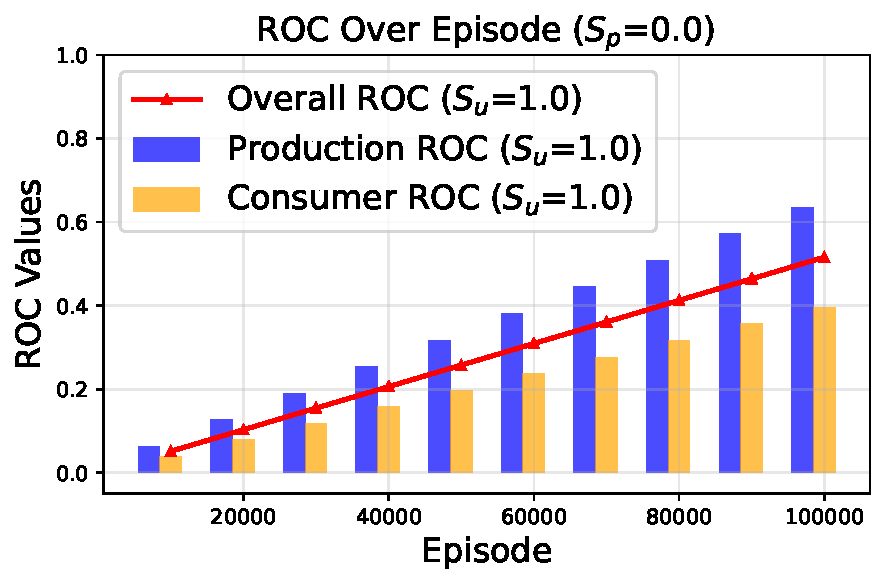
\includegraphics[width=\linewidth]{figures/fixed_sp/population_strategy_0_0_roc.pdf}
    \end{subfigure}
    \begin{subfigure}[b]{0.162\linewidth}
        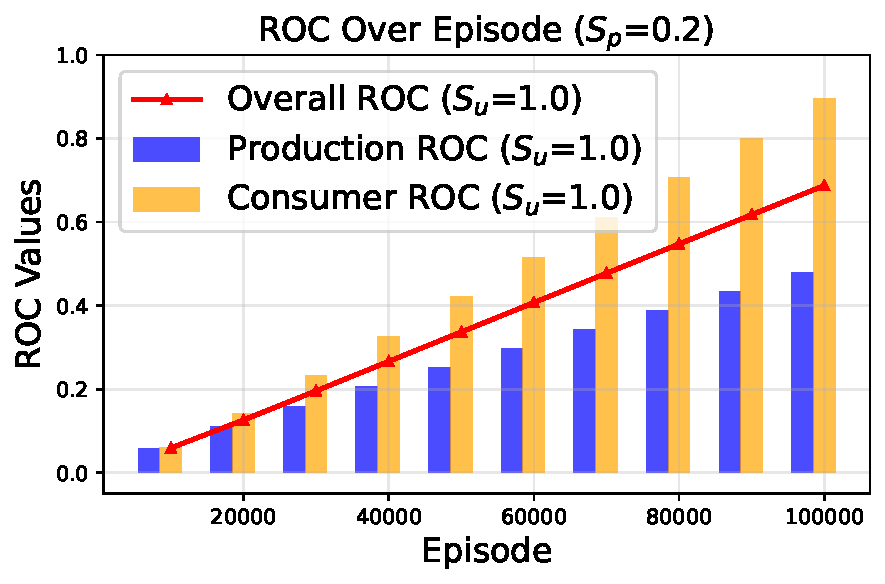
\includegraphics[width=\linewidth]{figures/fixed_sp/population_strategy_0_2_roc.pdf}
    \end{subfigure}
    \begin{subfigure}[b]{0.162\linewidth}
        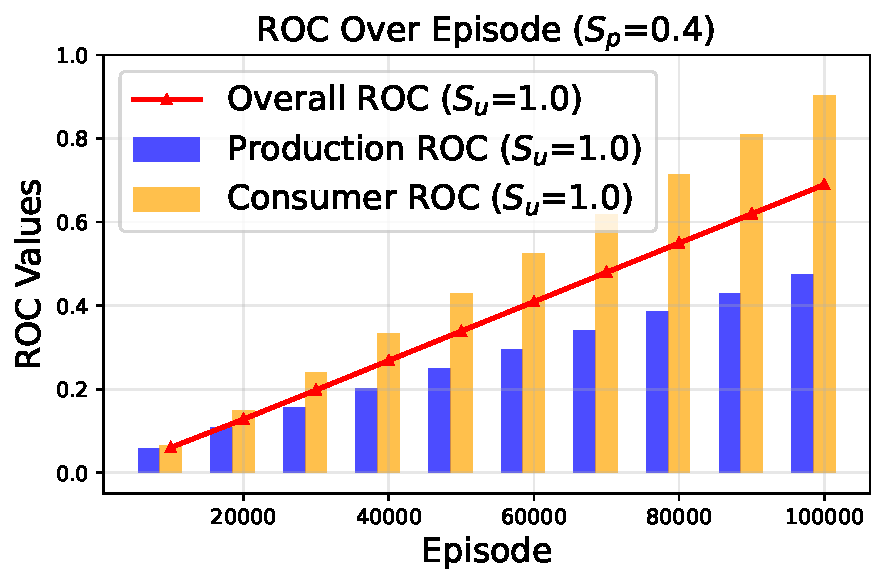
\includegraphics[width=\linewidth]{figures/fixed_sp/population_strategy_0_4_roc.pdf}
    \end{subfigure}
    \begin{subfigure}[b]{0.162\linewidth}
        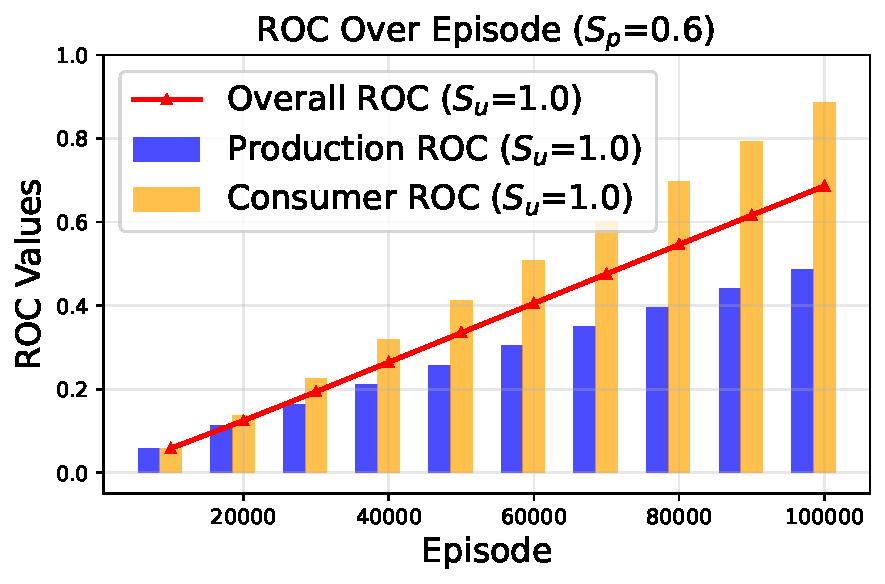
\includegraphics[width=\linewidth]{figures/fixed_sp/population_strategy_0_6_roc.pdf}
    \end{subfigure}
    \begin{subfigure}[b]{0.162\linewidth}
        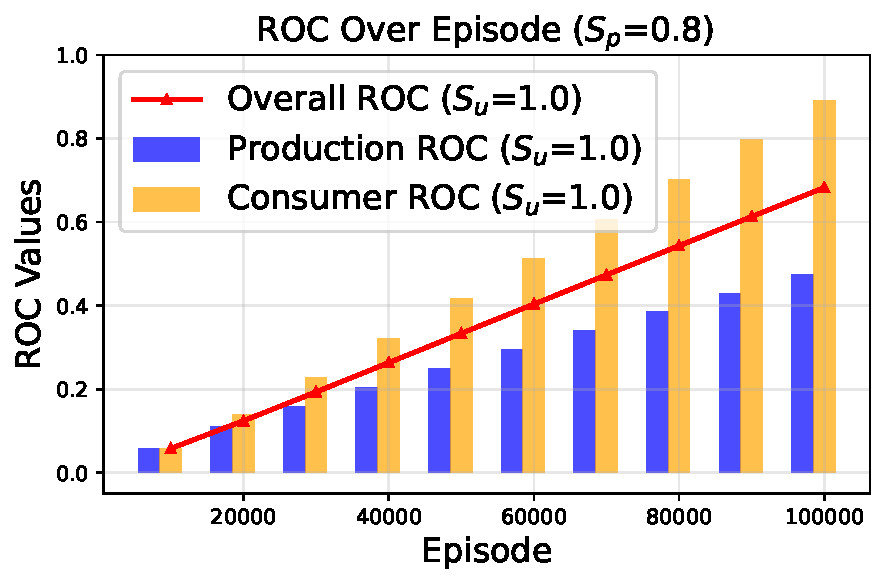
\includegraphics[width=\linewidth]{figures/fixed_sp/population_strategy_0_8_roc.pdf}
    \end{subfigure}
    \begin{subfigure}[b]{0.162\linewidth}
        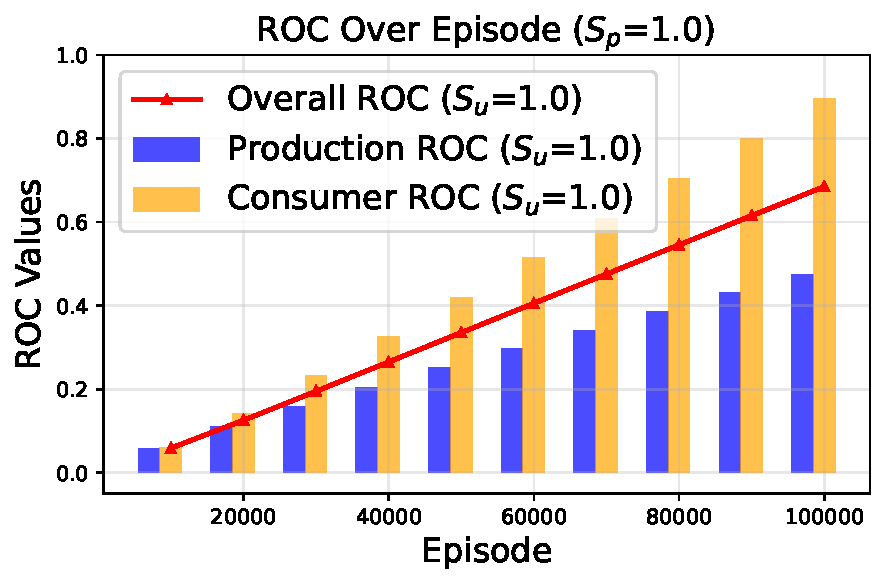
\includegraphics[width=\linewidth]{figures/fixed_sp/population_strategy_1_0_roc.pdf}
    \end{subfigure}
    \vspace{1mm}
    \begin{subfigure}[b]{0.162\linewidth}
        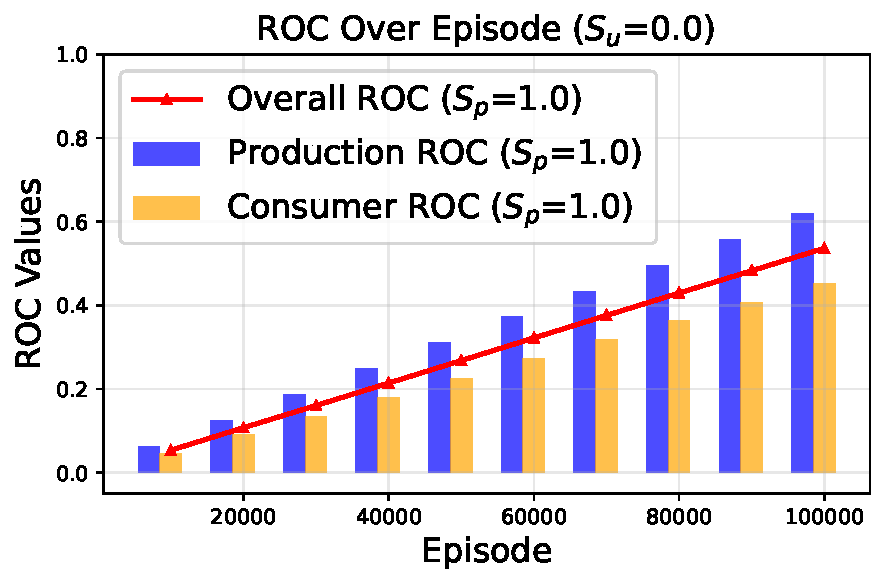
\includegraphics[width=\linewidth]{figures/fixed_su/user_strategy_0_0_roc.pdf}
    \end{subfigure}
    \begin{subfigure}[b]{0.162\linewidth}
        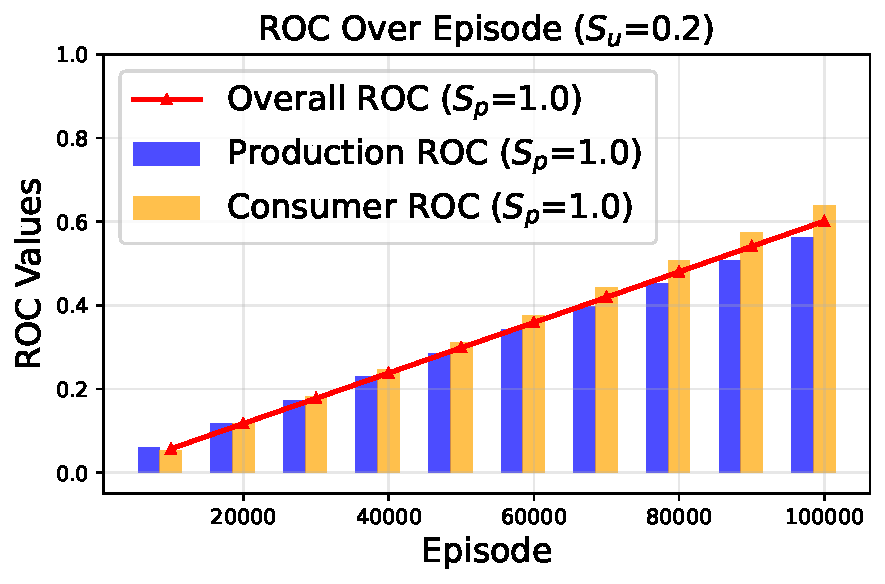
\includegraphics[width=\linewidth]{figures/fixed_su/user_strategy_0_2_roc.pdf}
    \end{subfigure}
    \begin{subfigure}[b]{0.162\linewidth}
        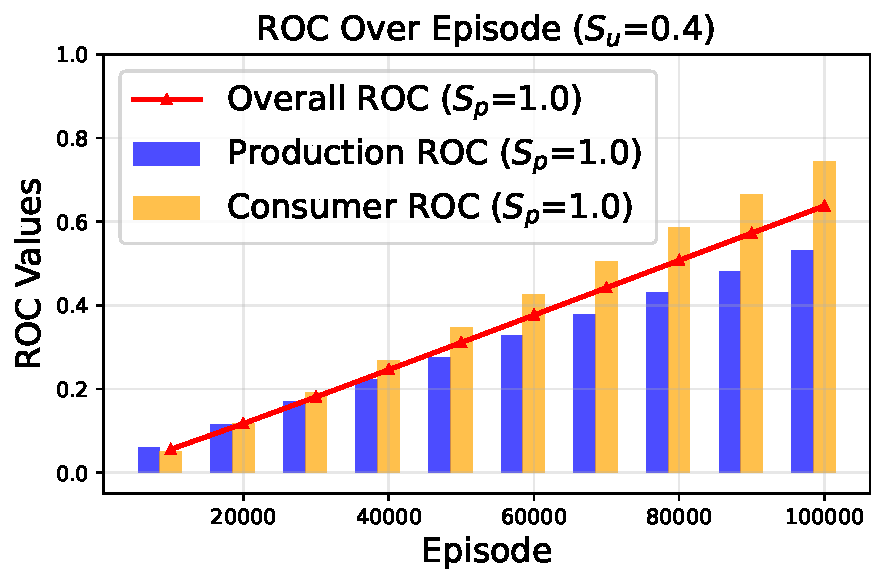
\includegraphics[width=\linewidth]{figures/fixed_su/user_strategy_0_4_roc.pdf}
    \end{subfigure}
    \begin{subfigure}[b]{0.162\linewidth}
        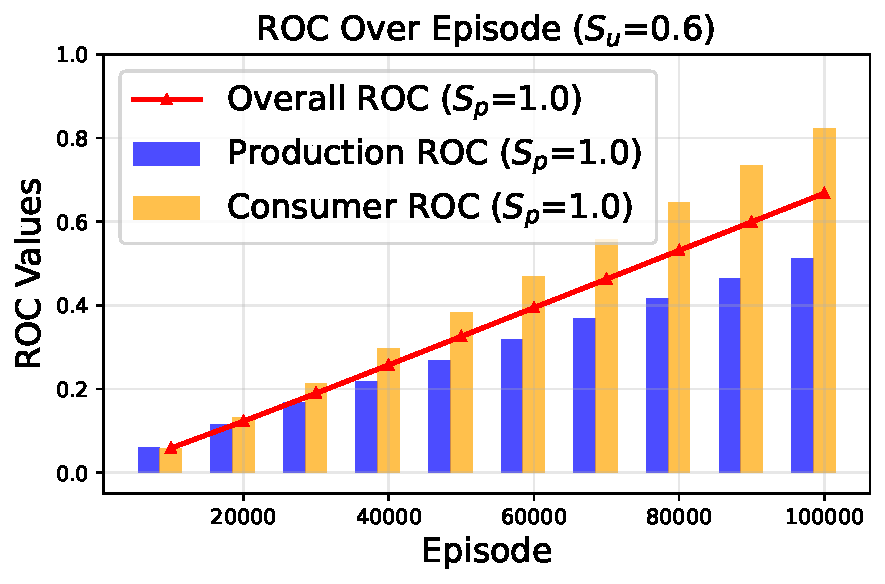
\includegraphics[width=\linewidth]{figures/fixed_su/user_strategy_0_6_roc.pdf}
    \end{subfigure}
    \begin{subfigure}[b]{0.162\linewidth}
        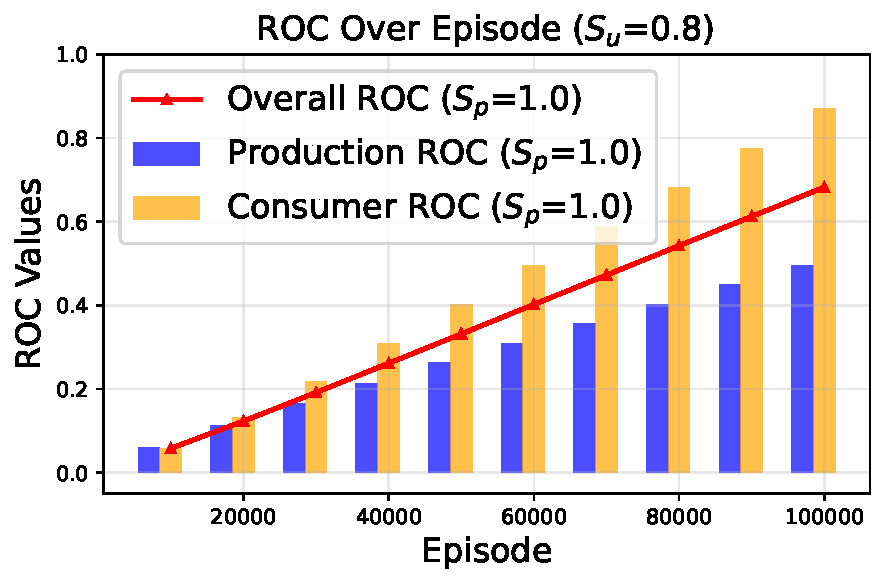
\includegraphics[width=\linewidth]{figures/fixed_su/user_strategy_0_8_roc.pdf}
    \end{subfigure}
    \begin{subfigure}[b]{0.162\linewidth}
        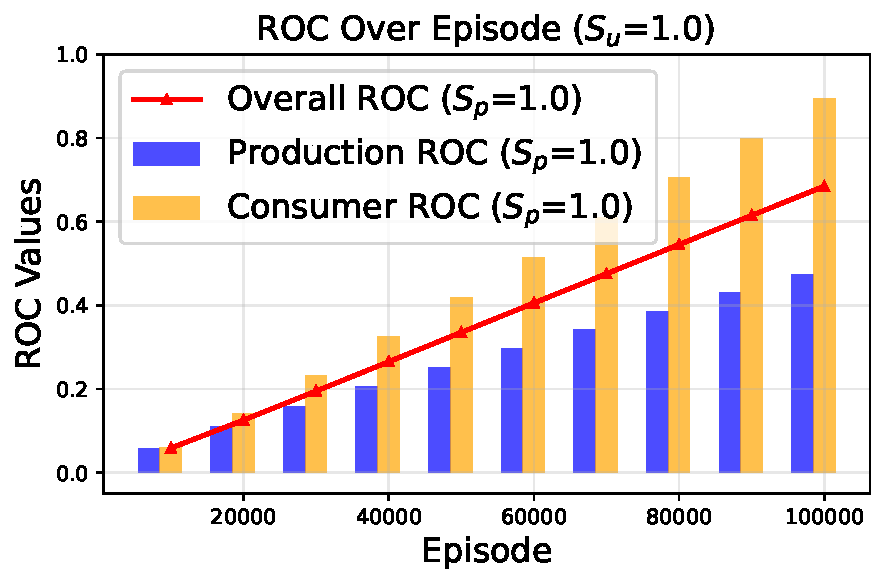
\includegraphics[width=\linewidth]{figures/fixed_su/user_strategy_1_0_roc.pdf}
    \end{subfigure}
    \vspace{-4mm}
    \caption{ROC comparison over 100,000 episodes under different strategy configurations. Top row: varying $S_p$ (proportion of rational agents) with $S_u = 1$. Bottom row: varying $S_u$ (strategy update probability) with $S_p = 1$.}
    \label{fig:roc_comp}
    \vspace{-1mm}
\end{figure*}

\begin{figure*}[t]
    \centering
    \begin{subfigure}[b]{0.162\linewidth}
        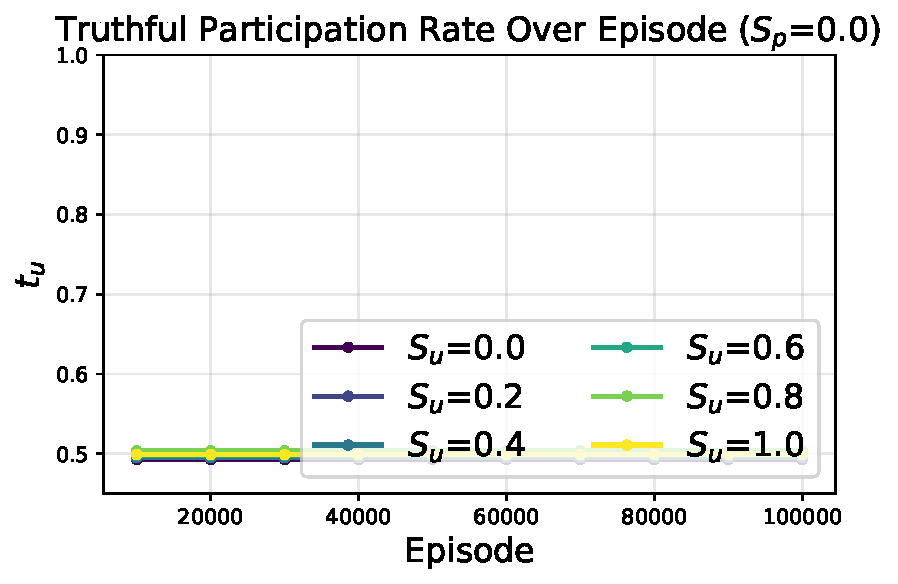
\includegraphics[width=\linewidth]{figures/fixed_sp/population_strategy_0_0_hard.pdf}
    \end{subfigure}
    \begin{subfigure}[b]{0.162\linewidth}
        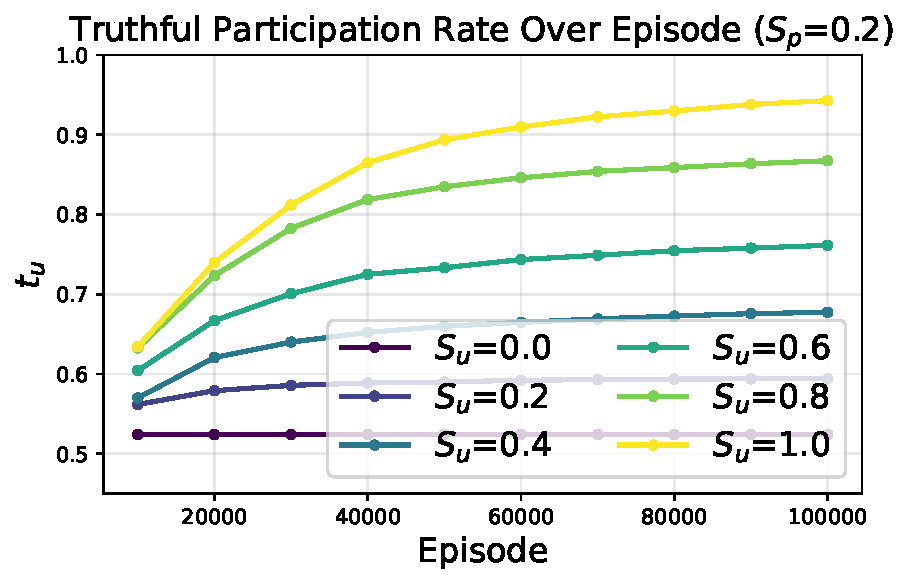
\includegraphics[width=\linewidth]{figures/fixed_sp/population_strategy_0_2_hard.pdf}
    \end{subfigure}
    \begin{subfigure}[b]{0.162\linewidth}
        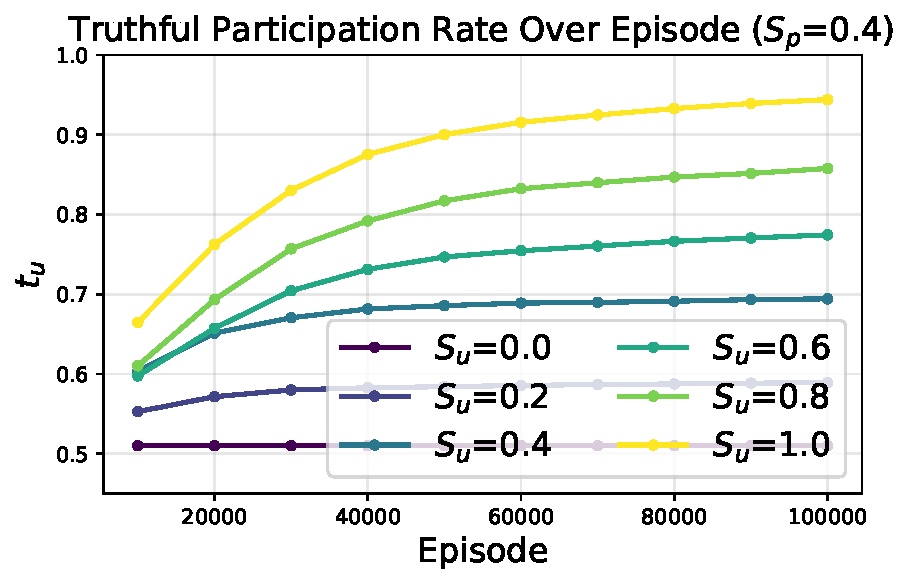
\includegraphics[width=\linewidth]{figures/fixed_sp/population_strategy_0_4_hard.pdf}
    \end{subfigure}
    \begin{subfigure}[b]{0.162\linewidth}
        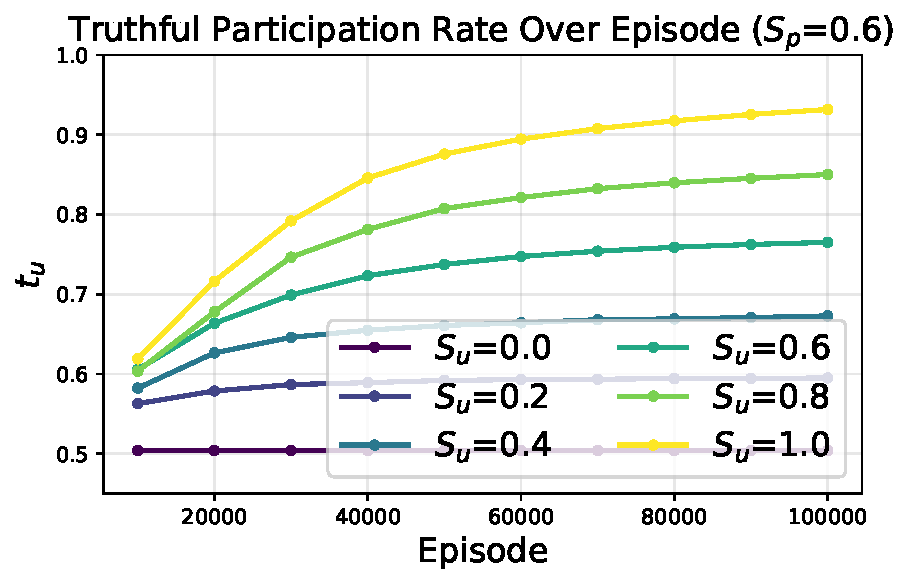
\includegraphics[width=\linewidth]{figures/fixed_sp/population_strategy_0_6_hard.pdf}
    \end{subfigure}
    \begin{subfigure}[b]{0.162\linewidth}
        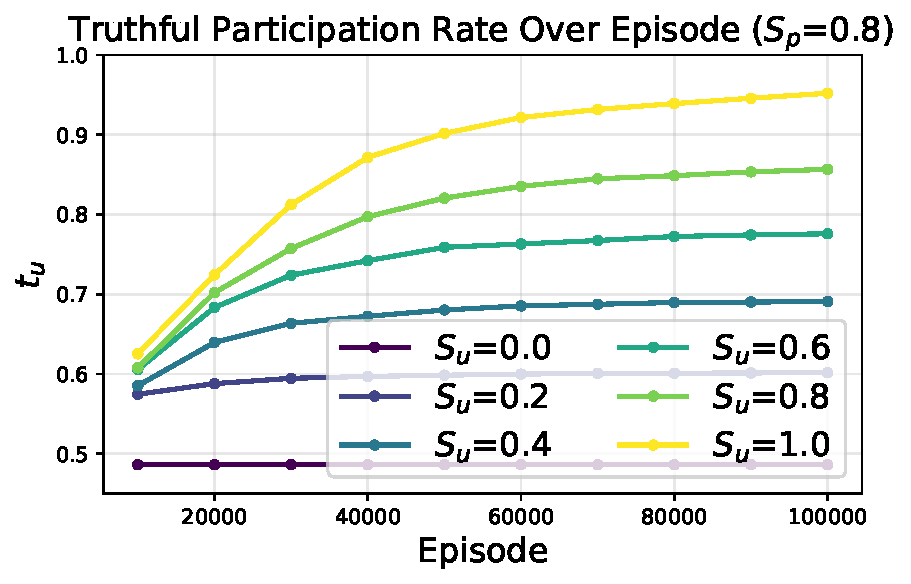
\includegraphics[width=\linewidth]{figures/fixed_sp/population_strategy_0_8_hard.pdf}
    \end{subfigure}
    \begin{subfigure}[b]{0.162\linewidth}
        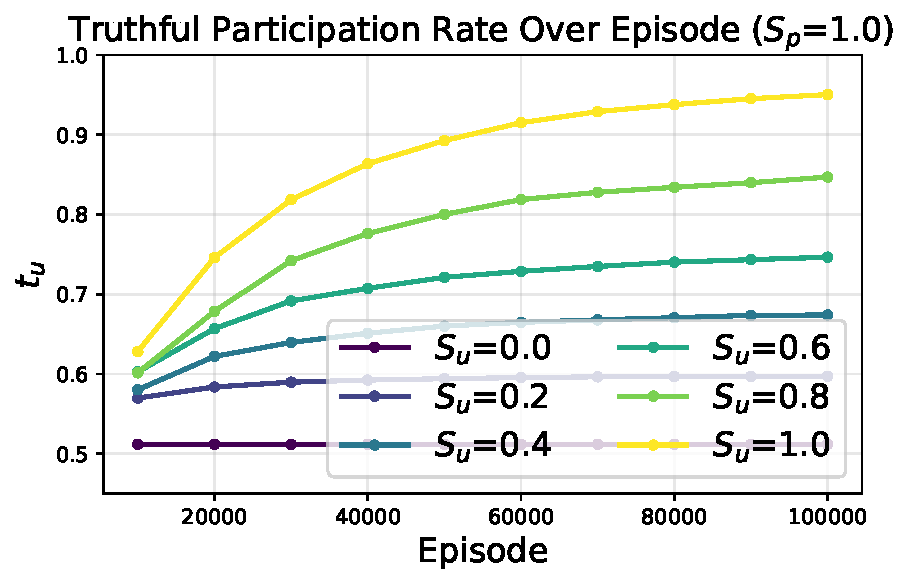
\includegraphics[width=\linewidth]{figures/fixed_sp/population_strategy_1_0_hard.pdf}
    \end{subfigure}
    \vspace{1mm}
    \begin{subfigure}[b]{0.162\linewidth}
        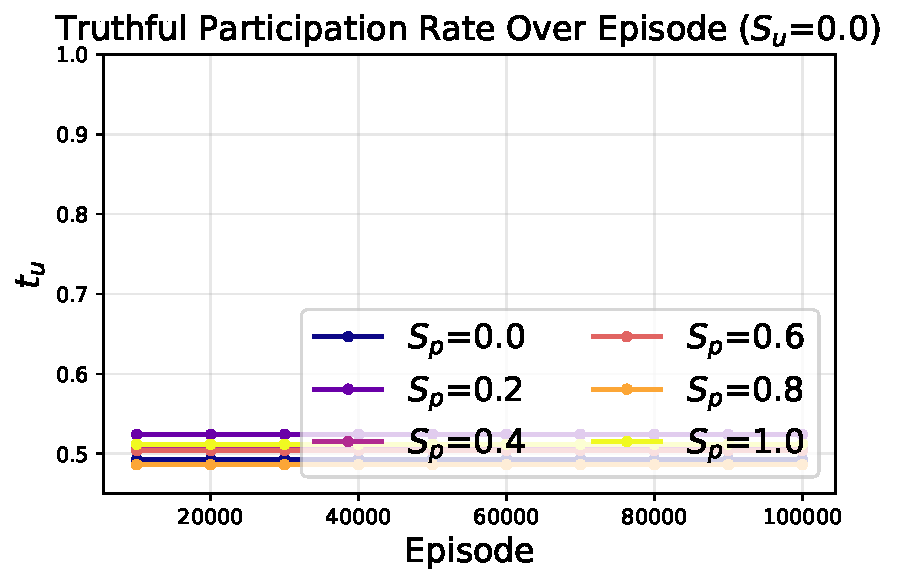
\includegraphics[width=\linewidth]{figures/fixed_su/user_strategy_0_0_hard.pdf}
    \end{subfigure}
    \begin{subfigure}[b]{0.162\linewidth}
        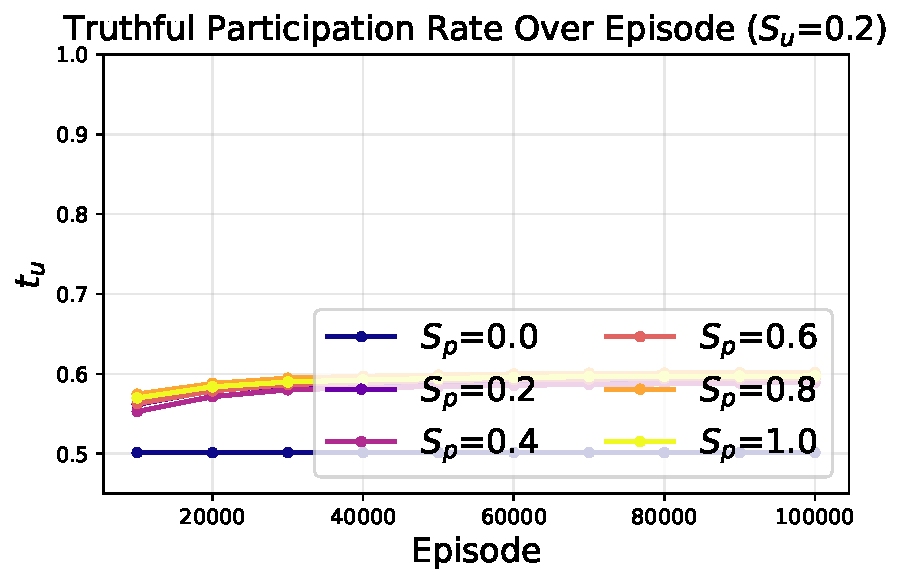
\includegraphics[width=\linewidth]{figures/fixed_su/user_strategy_0_2_hard.pdf}
    \end{subfigure}
    \begin{subfigure}[b]{0.162\linewidth}
        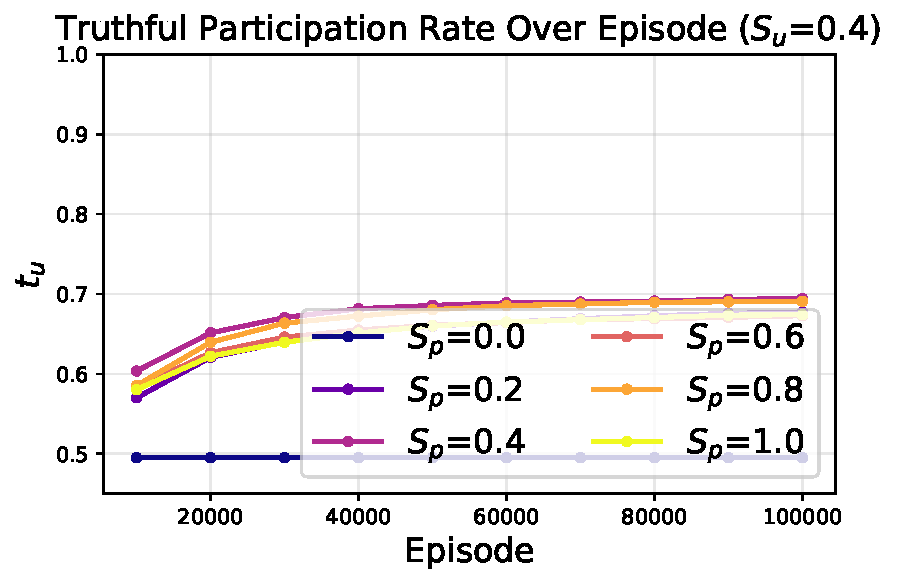
\includegraphics[width=\linewidth]{figures/fixed_su/user_strategy_0_4_hard.pdf}
    \end{subfigure}
    \begin{subfigure}[b]{0.162\linewidth}
        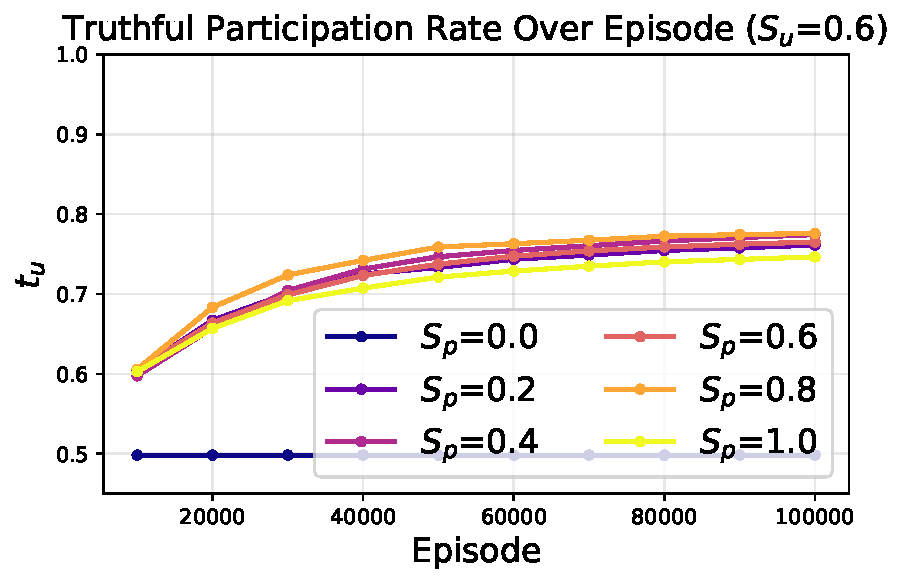
\includegraphics[width=\linewidth]{figures/fixed_su/user_strategy_0_6_hard.pdf}
    \end{subfigure}
    \begin{subfigure}[b]{0.162\linewidth}
        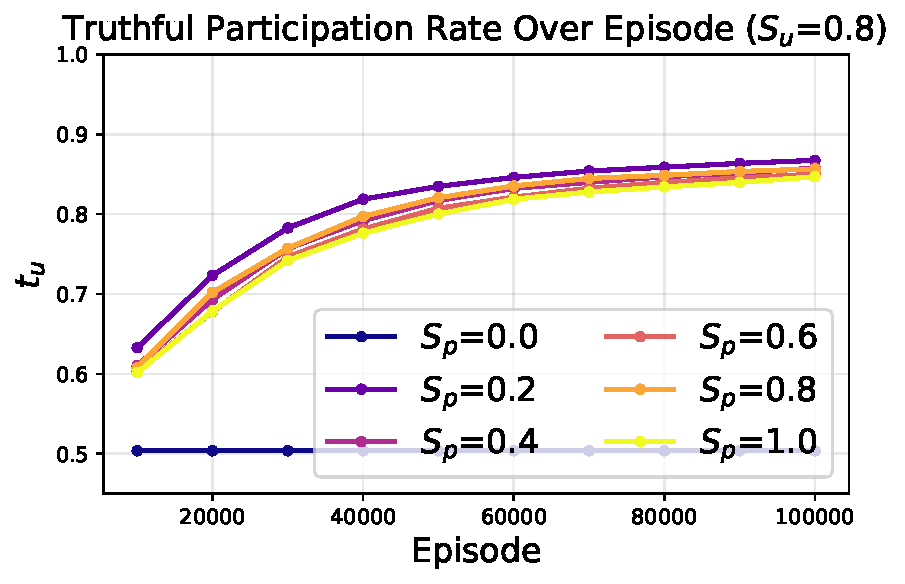
\includegraphics[width=\linewidth]{figures/fixed_su/user_strategy_0_8_hard.pdf}
    \end{subfigure}
    \begin{subfigure}[b]{0.162\linewidth}
        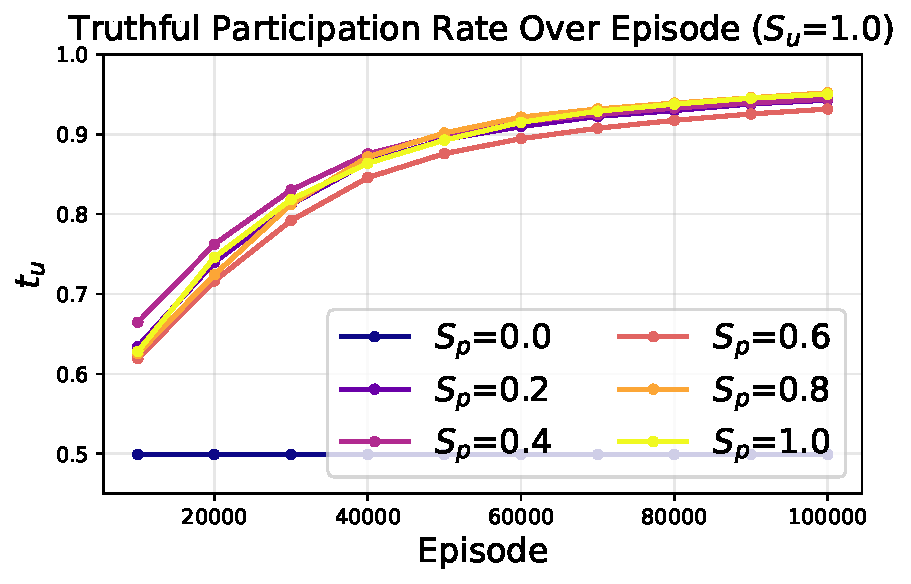
\includegraphics[width=\linewidth]{figures/fixed_su/user_strategy_1_0_hard.pdf}
    \end{subfigure}
    \vspace{-3mm}
    \caption{Truthful participation rate comparison under different $S_u$ and $S_p$ configurations. As rational agents increase ($S_p \uparrow$) and update their strategies more frequently ($S_u \uparrow$), the population converges toward higher truthful participation.}
    \label{fig:truthful_participation}
\end{figure*}


% =========================================================================
\subsection{Case Study: Decentralized Question Answering (DeQA)}
\label{sec:case_study}
% =========================================================================

The theoretical analysis above establishes that the ecosystem admits a self-enforcing equilibrium under appropriate parameter conditions.
We now ask: \textit{do these predictions hold in practice?}
Specifically, we seek to verify three empirical implications of the theory:
(i) that rational agents converge toward truthful strategies under the tokenomics--knowledge dual loop (predicted by the IC and IR conditions);
(ii) that the validation mechanism improves welfare, with performance depending on committee size $n$ (predicted by the comparative statics of Theorem~\ref{Strict IC for Validators});
and (iii) that the mechanism amplifies genuine quality but cannot compensate for fundamentally unreliable agents (predicted by the MLRP-based threshold structure of Theorems~\ref{IR for Producers}--\ref{IR-based Policy for Consumers}).

To test these predictions, we instantiate the ecosystem as a \textbf{De}centralized \textbf{Q}uestion \textbf{A}nswering system (\textbf{DeQA}).
Question answering serves as a natural testbed: consumer agents issue domain-specific queries, producer agents provide answers drawing on their knowledge bases, and validator agents independently generate answers and compare them against the producer's output to assess service alignment.
While we use QA for concreteness, we emphasize that the mechanism design, theoretical results, and incentive structures are domain-agnostic and apply to any knowledge-intensive agent collaboration scenario (e.g., code generation, data analysis, research synthesis).

These empirical implications motivate three research questions:

$\bullet$~\textbf{RQ1} (Rationality and Evolution): How do agent strategies influence ecosystem evolution?

$\bullet$~\textbf{RQ2} (Validation Mechanism): How does the number of validators affect net welfare?

$\bullet$~\textbf{RQ3} (Service Quality): What is the relationship between service quality and overall welfare?


\begin{figure*}[t]
    \centering
    \vspace{-6mm}
    \begin{subfigure}[b]{0.195\linewidth}
        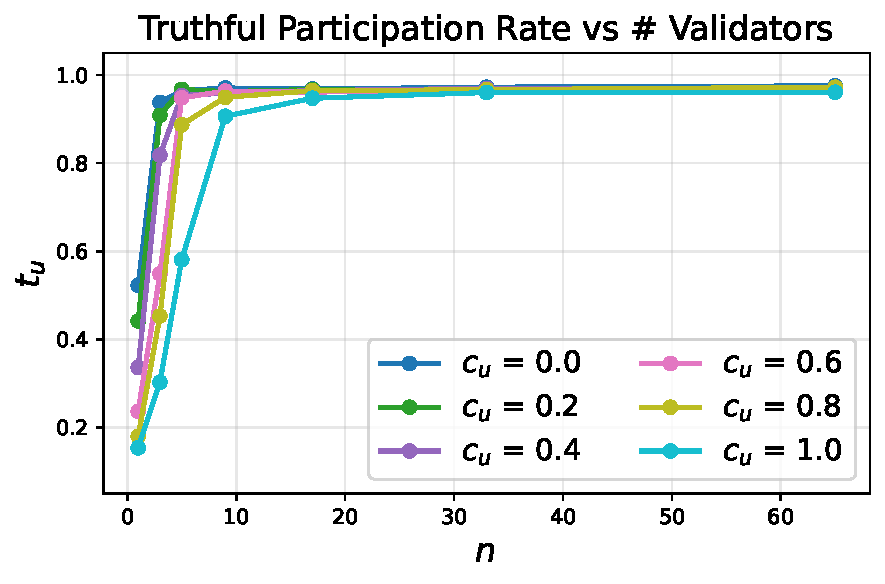
\includegraphics[width=\linewidth]{figures/hard/hard_all_costs.pdf}
        \caption{Truthful Participation}
    \end{subfigure}
    \hfill
    \begin{subfigure}[b]{0.195\linewidth}
        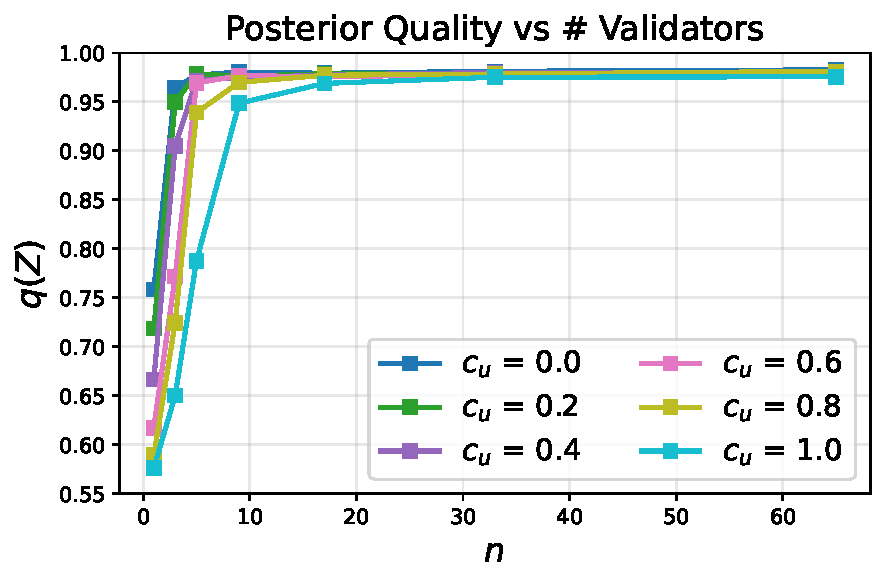
\includegraphics[width=\linewidth]{figures/hard/weighted_p_all_costs.pdf}
        \caption{Posterior Quality}
    \end{subfigure}
    \hfill
    \begin{subfigure}[b]{0.195\linewidth}
        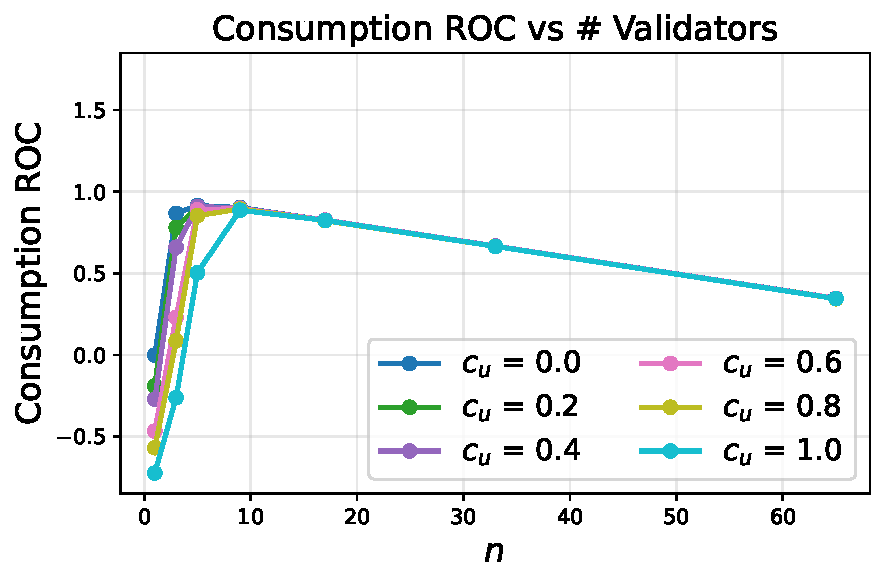
\includegraphics[width=\linewidth]{figures/hard/consumer_roc_all_costs.pdf}
        \caption{Consumption ROC}
    \end{subfigure}
    \hfill
    \begin{subfigure}[b]{0.195\linewidth}
        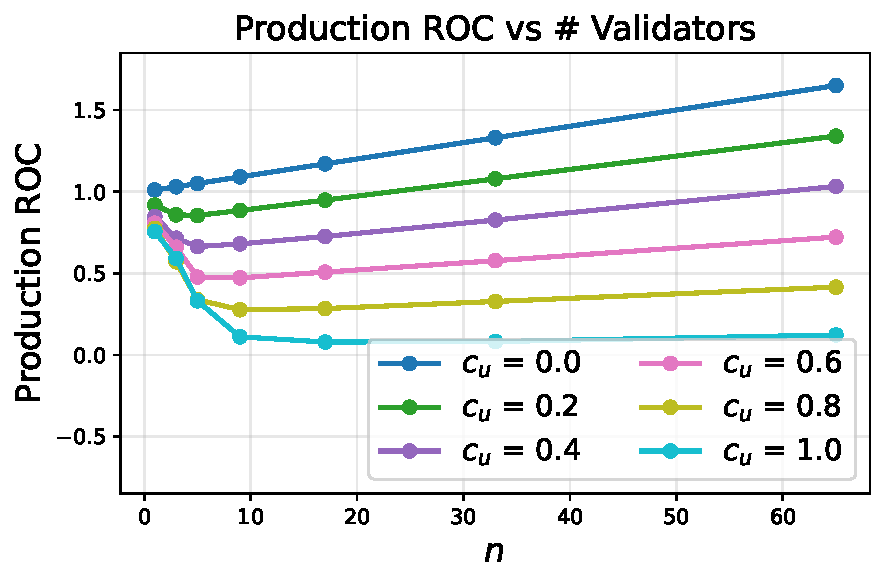
\includegraphics[width=\linewidth]{figures/hard/validator_roc_all_costs.pdf}
        \caption{Production ROC}
    \end{subfigure}
    \hfill
    \begin{subfigure}[b]{0.195\linewidth}
        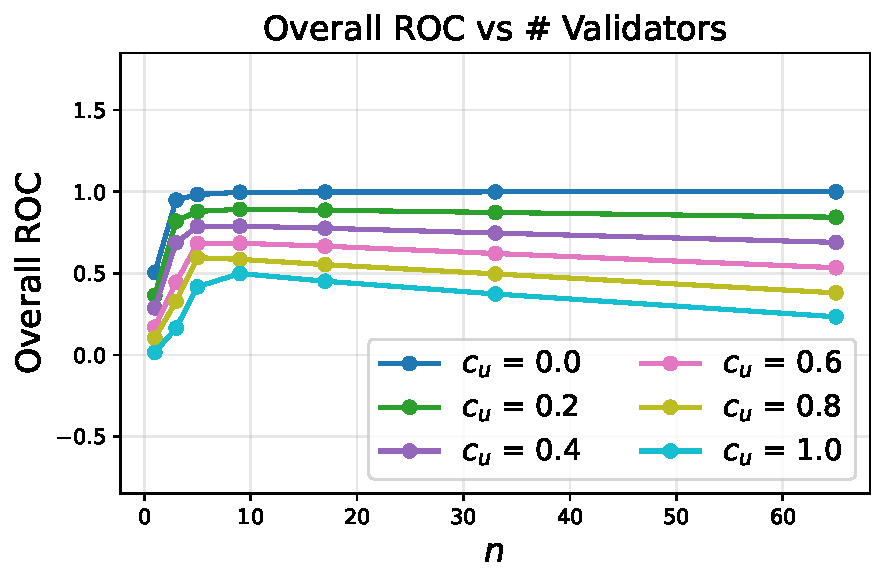
\includegraphics[width=\linewidth]{figures/hard/total_roc_all_costs.pdf}
        \caption{Overall ROC}
    \end{subfigure}
    \vspace{-2mm}
    \caption{Performance under different effort costs and validator counts. Larger committees improve posterior quality and consumer welfare up to a point, after which diminishing returns from increased validation cost reduce total welfare.}
    \label{fig:cost_validators}
    \vspace{0mm}
\end{figure*}

\begin{figure*}[t]
    \centering
    \begin{subfigure}[b]{0.15\linewidth}
        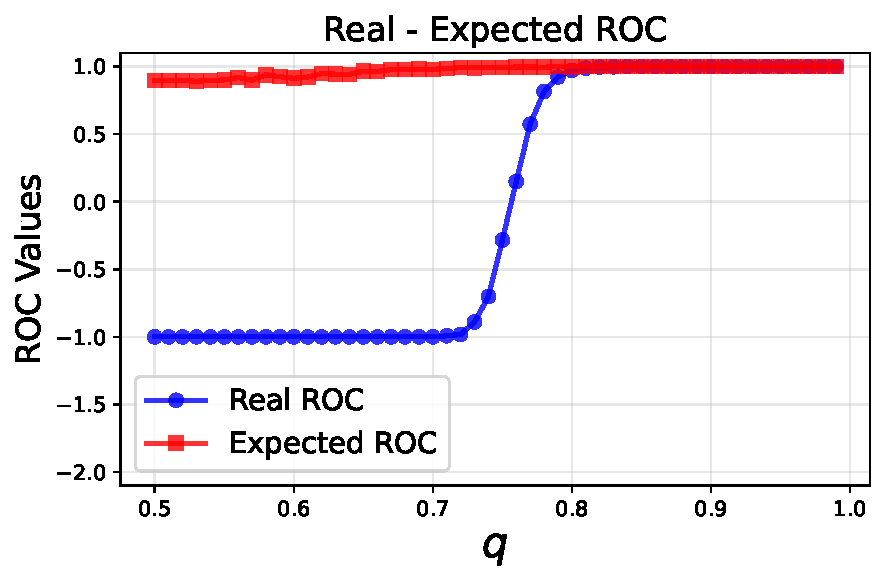
\includegraphics[width=\linewidth]{figures/quality/real_expected_roc_vs_p.pdf}
        \caption{Real ROC - \\Expected ROC}
    \end{subfigure}
    \begin{subfigure}[b]{0.15\linewidth}
        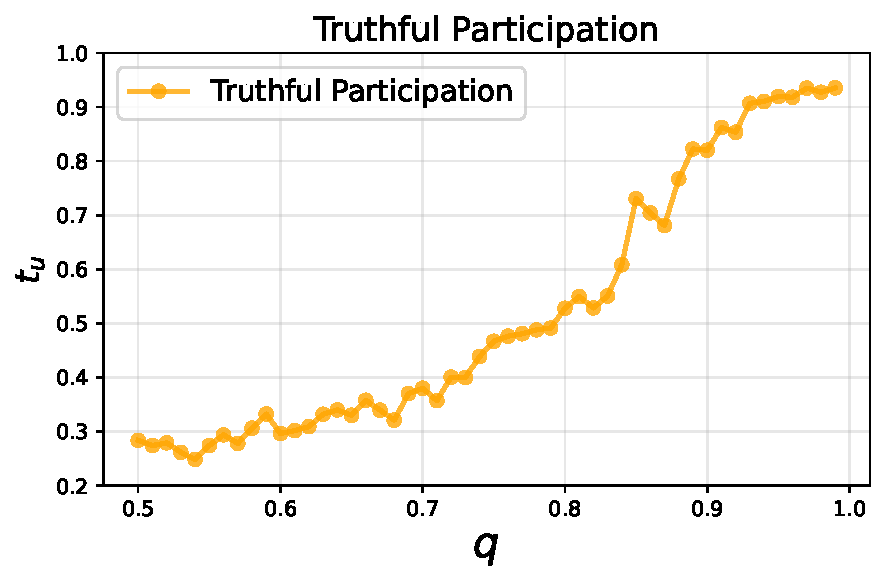
\includegraphics[width=\linewidth]{figures/quality/truthful_participation_vs_p.pdf}
        \caption{\textbf{\footnotesize Truthful \\Participation}}
    \end{subfigure}
    \begin{subfigure}[b]{0.15\linewidth}
        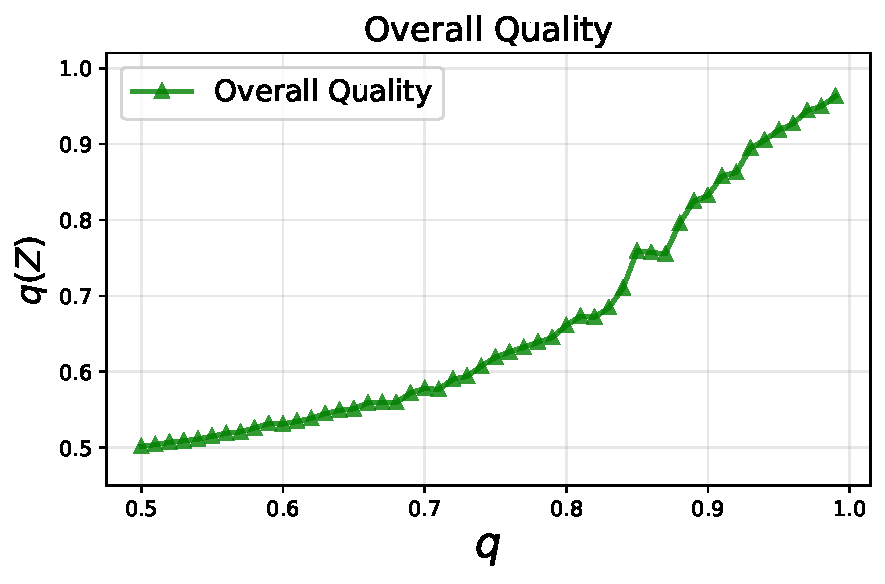
\includegraphics[width=\linewidth]{figures/quality/posterior_quality_vs_p.pdf}
        \caption{Overall \\Quality}
    \end{subfigure}
    \begin{subfigure}[b]{0.15\linewidth}
        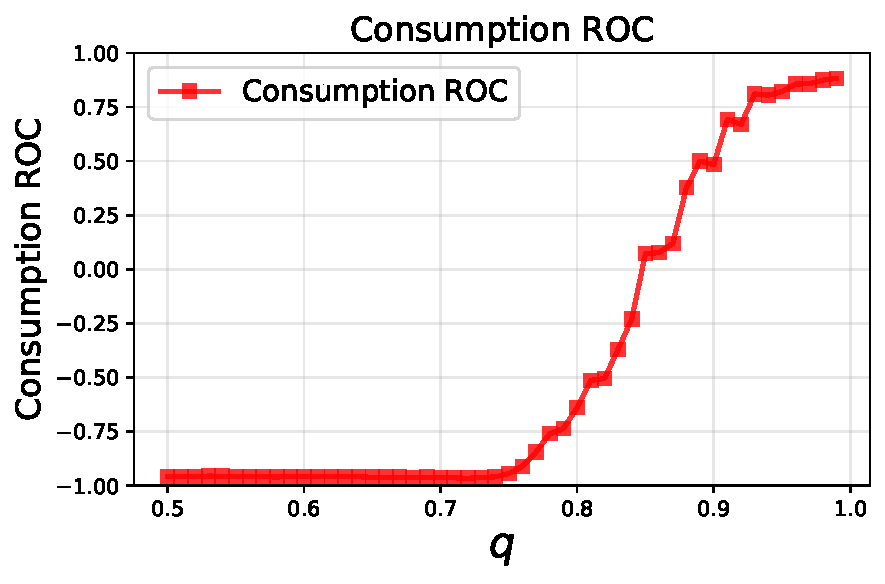
\includegraphics[width=\linewidth]{figures/quality/consumption_roc_vs_p.pdf}
        \caption{Consumption \\ROC}
    \end{subfigure}
    \begin{subfigure}[b]{0.15\linewidth}
        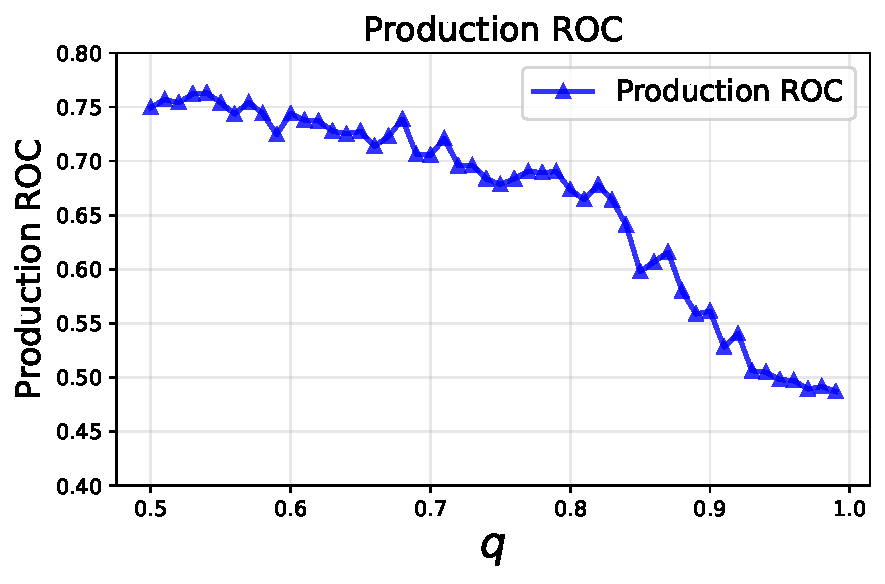
\includegraphics[width=\linewidth]{figures/quality/production_roc_vs_p.pdf}
        \caption{Production \\ROC}
    \end{subfigure}
    \begin{subfigure}[b]{0.15\linewidth}
        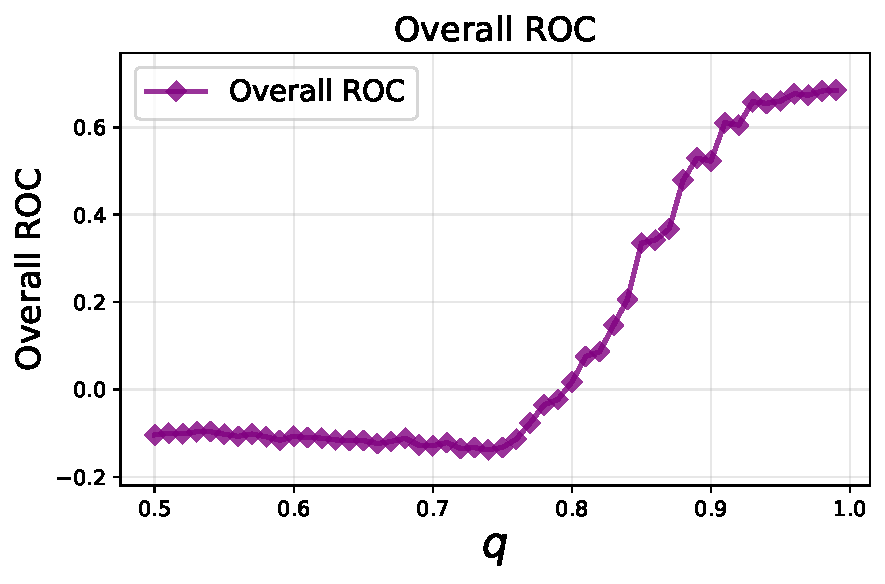
\includegraphics[width=\linewidth]{figures/quality/total_roc_vs_p.pdf}
        \caption{Overall \\ROC}
    \end{subfigure}
    \vspace{-2mm}
    \caption{Performance under different service quality levels. When producer quality is low ($q \approx 0.5$), the incentive mechanism cannot compensate, and welfare collapses. As quality increases, the mechanism amplifies honest effort into ecosystem-wide gains.}
    \label{fig:quality_impact}
\end{figure*}


\subsubsection{Instantiation}
In DeQA, the abstract ecosystem roles map to the QA domain as follows.
Consumer agents issue domain-specific \textit{queries} (e.g., medical, legal, scientific).
Producer agents provide \textit{answers} by invoking their knowledge-intensive service $a_u: \mathcal{Q} \rightarrow \mathcal{R}$, where $\mathcal{Q}$ is the query space and $\mathcal{R}$ the answer space.
Validator agents independently generate answers to the same queries and compare them against the producer's output, voting on agreement/disagreement to form the PoI consensus.
Service quality $q$ denotes the probability of generating a correct answer for a given query.


\subsubsection{Simulation Setting}

The simulation parameters are chosen to satisfy the theoretical assumptions while reflecting realistic operating conditions. We explain each choice and its connection to the formal model.

\textbf{(1) Agents and Roles.}
The system contains $N = 10{,}000$ agents, each randomly assuming the role of consumer, producer, or validator in each round.
Consumers issue queries uniformly across domains.
Agent service quality follows $q \sim 0.98 + 0.02\,\mathrm{Beta}(4,4) > \frac{1}{2}$, ensuring that Assumption~\ref{assum:validators} ($q_v > \frac{1}{2}$) is satisfied for all agents.
The Beta(4,4) distribution concentrates quality near the mean while allowing meaningful variance, modeling a population of generally competent but heterogeneous agents.
Agents selected randomly (without effort) have $q = \frac{1}{2}$, corresponding to the shirking case in Assumption~\ref{assum:binary}.
Each agent starts with $2{,}000$ tokens and exits once depleted, creating the finite-resource pressure that drives evolutionary dynamics.

\textbf{(2) Validation Mechanism.}
Validator count $n$ is odd (as required by Assumption~\ref{assum:validators}) and varied across $\{1, 5, 9, 17, 33, 65\}$ to test the comparative statics prediction that larger $n$ strengthens IC by raising $P_{\text{match}}$.
Each validation uses $m = 10$ sample queries, providing sufficient statistical power for consensus.
Validation fee $\tau_{\text{val}} = 1$ and stake $\sigma = 1$, satisfying $c_u < \tau_{\text{val}}$ (Assumption~\ref{assum:costs}) for all effort costs in our range.
Consensus is by majority vote, consistent with the theoretical model.
Each agent's strategy is parameterized by its truthful participation rate $t_u \in [0, 1]$ in both production and validation---when $t_u = 1$, the agent always exerts full effort ($e = 1$ in the formal model); when $t_u = 0$, it always shirks ($e = 0$).
Agents aim to maximize return on capital (ROC); low-ROC agents learn strategies from high-ROC agents, modeling the rational adaptive behavior predicted by the BNE dynamics.
Initial strategies are random ($t_u = \text{Uniform}(0, 1)$), representing a ``cold start'' ecosystem with no prior coordination.

\textbf{(3) Promotion and Subscription.}
Producers incur effort cost $c_u \in (0, 1)$ per validation query and receive $\tau_s = 1{,}000$ upon successful subscription.
The large ratio $\tau_s / \tau_{\text{val}} = 1{,}000$ ensures the cost ordering $mn\tau_{\text{val}} \ll \tau_s$ required by Assumption~\ref{assum:costs}, making validation economically viable relative to the subscription stakes.

\textbf{(4) System Assumptions and Simulation Protocol.}
Validators are independent and non-collusive (Assumption~\ref{assum:validators}). All parameters are finite and drawn from bounded intervals.
We simulate 100{,}000 \textit{interaction episodes}, where each episode constitutes one complete promotion--validation--subscription cycle: a consumer broadcasts a service need, a producer promotes, validators assess, and the consumer decides whether to subscribe.
Results are averaged over 5 independent random seeds; shaded regions in figures indicate $\pm 1$ standard deviation.

\textbf{(5) Evaluation Metrics.}
We evaluate three metrics, defined formally as follows:
\begin{itemize}
    \item \textbf{Truthful participation rate} $\bar{t} \coloneqq \frac{1}{|\mathcal{U}_{\text{active}}|} \sum_{u \in \mathcal{U}_{\text{active}}} t_u$, the population-averaged effort level.
    \item \textbf{Return on capital (ROC)}: for each agent $u$, $\text{ROC}_u \coloneqq (B_u^{\text{final}} - B_u^{\text{init}}) / B_u^{\text{init}}$, where $B_u^{\text{init}}$ and $B_u^{\text{final}}$ are the agent's initial and final token balances. Aggregate ROC is computed separately for consumers, producers, and the total population.
    \item \textbf{Social welfare} $W \coloneqq \sum_{u \in \mathcal{U}} \text{ROC}_u$, the sum of all agents' returns on capital, capturing the total economic surplus generated by the ecosystem. We also report consumer welfare $W_c$ and producer welfare $W_p$ to characterize surplus distribution.
    \item \textbf{Posterior quality} $\mathbb{E}[q_p \mid Z = 1]$, the expected producer quality conditional on passing validation, measuring the informativeness of the PoI mechanism.
\end{itemize}

\textbf{(6) Rationality Parameters.}
To study convergence \textit{toward} the BNE (rather than assuming agents start at equilibrium), we parameterize the population's rationality via two variables: $S_p \in [0, 1]$ denotes the proportion of agents that follow a rational learning rule (the remainder play fixed random strategies), and $S_u \in [0, 1]$ denotes the probability that a rational agent updates its strategy in a given round by imitating a higher-ROC peer. The case $S_p = S_u = 1$ corresponds to a fully adaptive population; $S_p = 0$ corresponds to a frozen, non-learning baseline.

\textbf{(7) Baselines.}
To contextualize our results, we compare against two natural baselines derived from the simulation itself:
\begin{itemize}
    \item \textbf{No-PoI} ($n = 0$): consumers subscribe based solely on the producer's self-reported performance declaration, without any third-party validation. This represents the information-asymmetry regime where the ``market for lemons'' operates unchecked.
    \item \textbf{Single-Validator} ($n = 1$): a single validator assesses service quality. As our IC analysis predicts (Theorem~\ref{Strict IC for Validators}), the lone validator faces minimal competitive pressure and is prone to shirking, since $P_{\text{match}} = q_v$ offers only a marginal advantage over random voting.
\end{itemize}
These baselines are not separate experiments but correspond to the boundary cases of our parameterized simulation, allowing direct comparison within the same experimental framework.

\subsubsection{Agent Rationality and Community Evolution (RQ1)}

We examine how the rationality parameters $S_p$ (proportion of adaptive agents) and $S_u$ (strategy update probability) influence ecosystem dynamics.

As shown in Figure~\ref{fig:roc_comp}, when agents never update strategies ($S_u = 1$, $S_p = 0$), producer surplus exceeds consumer surplus, but overall welfare remains low.
This baseline represents a ``frozen'' ecosystem where no learning occurs---producers who happen to shirk continue shirking, and consumers bear the cost of unreliable services.

When rational producers begin adapting by increasing $t_u$ (Figures~\ref{fig:roc_comp} and~\ref{fig:truthful_participation}), a striking pattern emerges:
individual producer surplus \textit{decreases} (higher effort means higher cost), but consumer surplus and total social welfare \textit{increase substantially}.
Low-ROC agents observe the success of high-$t_u$ agents and imitate their strategies, creating a population-level convergence toward honest participation.

\textbf{Theoretical connection.}
This result empirically confirms the tokenomics--knowledge dual loop: the incentive mechanism channels rational self-interest into collective welfare improvement.
Producers invest in truthful effort not out of altruism but because the mechanism makes honesty the utility-maximizing strategy---precisely the IC condition of Theorem~\ref{Strict IC for Validators} and the self-screening of Theorem~\ref{IR for Producers} in action.
The ecosystem acts as an evolutionary engine: agents that invest in quality thrive, while those that shirk are outcompeted and gradually exit.


\subsubsection{Validation Mechanism Analysis (RQ2)}

We analyze how committee size $n$ affects truthful participation, posterior quality, and welfare distribution.

\textbf{The monopoly problem ($n = 1$).}
As shown in Figure~\ref{fig:cost_validators}(a), with a single validator, the IC condition is barely satisfied: $P_{\text{match}} = q_v$ offers only a marginal advantage over random voting, and the sole validator can directly determine the consensus.
The result is pervasive shirking, low posterior quality, and consumer welfare losses.

\textbf{The benefits of competition ($n \uparrow$).}
As $n$ increases, mutual supervision emerges: each validator knows that deviating from the majority risks stake forfeiture, because the remaining validators are likely to produce a correct consensus.
Truthful participation becomes the dominant strategy (Figure~\ref{fig:cost_validators}(b)), and posterior quality improves significantly---validating the comparative statics prediction that larger $n$ expands the IC region.

\textbf{The cost trade-off.}
Although validation quality improves monotonically with $n$, the total cost $mn\tau_{\text{val}}$ also increases linearly.
Consumer benefits exhibit diminishing marginal returns (each additional validator adds less incremental information), while costs grow linearly.
The result is a welfare-optimal committee size: social welfare and consumer surplus first increase then decline with $n$ (Figures~\ref{fig:cost_validators}(c)(e)), while producer surplus exhibits the inverse pattern (Figure~\ref{fig:cost_validators}(d)).
In our setting, moderate committee sizes $n \in \{5, 9, 17\}$ achieve the best trade-off.


\subsubsection{Service Quality Impacts (RQ3)}

Finally, we investigate the fundamental relationship between producer knowledge quality and ecosystem welfare.

As shown in Figure~\ref{fig:quality_impact}(a), when producer quality is uniformly low, validation outcomes deviate substantially from truth.
Consumers make subscription decisions based on incorrect signals and suffer welfare losses.
In the extreme case $q = 0.5$, producers are no better than random---they cannot earn higher incentives through reliable service and become increasingly idle (Figure~\ref{fig:quality_impact}(b)).
Both consumer surplus and overall welfare turn negative (Figures~\ref{fig:quality_impact}(d)(e)(f)), reflecting a collapsed market.

As $q$ increases, a qualitative transition occurs: producer effort begins receiving positive feedback from the mechanism.
Higher quality $\Rightarrow$ higher pass probability $V_p(q_p)$ $\Rightarrow$ higher subscription revenue $\Rightarrow$ stronger incentive to maintain quality.
This positive feedback loop stabilizes the incentive environment, driving consumer surplus and total welfare into sustained growth (Figures~\ref{fig:quality_impact}(c)(e)(f)).

\textbf{Core insight.}
This result illuminates a fundamental design principle: \textit{our ecosystem is designed to reveal and reward existing capability, not to create it from nothing.}
When agents possess genuine domain knowledge, the tokenomics mechanism amplifies honest effort into ecosystem-wide gains.
When the knowledge base is fundamentally unreliable ($q \approx 0.5$), no incentive mechanism can compensate---the ecosystem degrades regardless of the economic design.
This underscores the complementary nature of the ecosystem and the underlying agent capabilities: the mechanism provides the right incentives, but the agents must bring genuine knowledge to the table.


\section{Applications and Deployment Scenarios}
\label{sec:applications}

While we have instantiated the ecosystem as a decentralized question answering system (DeQA) for empirical validation, the underlying framework---three dynamically interchangeable roles, Proof-of-Intelligence validation, and tokenomics-driven incentive alignment---is fundamentally \textit{domain-agnostic}.
Any setting where (i)~agents possess heterogeneous domain expertise, (ii)~service quality is difficult to verify unilaterally, and (iii)~agents are deployed by independent organizations with potentially divergent interests, constitutes a natural deployment target.
We now survey a range of application domains, detailing how the ecosystem's mechanisms map to each context and what unique challenges and opportunities arise.


\subsection{Multi-Agent Software Engineering}

Modern software development increasingly involves autonomous agents that generate code, review pull requests, debug errors, and plan architectures~\cite{qian2023communicative, hong2023metagpt}.
In a decentralized ecosystem, \textit{producer} agents specialize in particular languages, frameworks, or codebases (e.g., a Rust systems programming agent, a React frontend agent, a database optimization agent), while \textit{consumer} agents route subtasks to the most capable specialist.
\textit{Validators} independently generate solutions or review the producer's code, comparing outputs to form a consensus on correctness, security, and adherence to specifications.

This domain is particularly well-suited to PoI because code correctness is partially verifiable: validators can execute test suites, run static analyzers, or compare behavioral outputs on sample inputs---providing a richer signal than pure textual comparison.
The architectural heterogeneity requirement maps naturally to using diverse code generation models (e.g., a CodeLlama-based validator assessing a GPT-4-generated solution), reducing the risk of correlated bugs from shared training biases.

A key deployment consideration is \textit{intellectual property}: organizations may be reluctant to expose proprietary codebases during validation.
The hybrid on-chain/off-chain architecture (\S\ref{sec:decentral_tech}) addresses this by keeping code artifacts off-chain while recording validation judgments and token settlements on-chain, preserving data sovereignty.


\subsection{Scientific Research and Discovery}

Scientific research increasingly relies on LLM agents for literature synthesis, hypothesis generation, experimental design, and data analysis~\cite{chen2023agentverse}.
In a decentralized research ecosystem, agents developed by different research institutions---each with expertise in distinct subfields---could collaborate across disciplinary boundaries.
A computational biology agent (consumer) seeking to model protein-drug interactions might subscribe to a quantum chemistry agent (producer) for binding energy calculations, with structural biology agents serving as validators.

The tokenomics--knowledge dual loop is especially compelling here: tokens earned from successful validations in one's area of expertise fund access to knowledge in areas where one lacks capability, creating a \textit{scientific knowledge economy} that incentivizes both deep specialization and broad collaboration.
The PoI mechanism could serve as a decentralized peer review proxy, where multiple independent agents assess the validity of a research claim before it is accepted and acted upon.

However, scientific domains present unique challenges for the binary signal model (Assumption~\ref{assum:binary}): research outputs are often nuanced, multi-dimensional, and not easily reduced to agree/disagree judgments.
Extending PoI to support graded or multi-dimensional validation signals is a promising direction (\S\ref{sec:future_work}).


\subsection{Healthcare and Clinical Decision Support}

Healthcare represents perhaps the highest-stakes deployment scenario.
Clinical decision support agents---specialized in radiology, pathology, pharmacology, or clinical trial analysis---are increasingly deployed by hospitals, pharmaceutical companies, and research institutions.
A primary care diagnostic agent (consumer) might seek a specialist opinion from a cardiology agent (producer), with independent clinical reasoning agents (validators) cross-checking the recommendation against evidence-based guidelines.

The trust crisis identified in \Cref{sec:trust_crisis} is particularly acute in healthcare: a mismatched subscription (i.e., relying on an unreliable specialist agent) can have life-threatening consequences.
The dual validation structure (promotion + subscription validation) provides a rigorous safety net, and the economic penalty for failed validation creates strong deterrence against agents that overstate their clinical competence.

Regulatory compliance adds a unique dimension: healthcare agents must satisfy jurisdiction-specific requirements (e.g., HIPAA in the US, GDPR in the EU) regarding data handling and patient privacy.
The decentralized infrastructure's data sovereignty guarantees---where patient data remains off-chain and under institutional control---align well with these requirements.
Moreover, the auditable consensus trail recorded on-chain provides regulatory bodies with a transparent record of how clinical recommendations were validated, potentially facilitating certification processes for AI-assisted medical decision-making.


\subsection{Legal Analysis and Compliance}

Legal reasoning requires deep domain expertise that varies dramatically across jurisdictions, practice areas, and regulatory regimes.
A corporate compliance agent (consumer) navigating cross-border regulations might subscribe to agents specializing in EU data protection law, US securities regulation, or Chinese antitrust law.
Validators with independent legal expertise assess whether the producer's analysis correctly interprets statutes, case law, and regulatory guidance.

The ecosystem's self-screening mechanism (Theorem~\ref{IR for Producers}) is particularly valuable here: the promotion fee acts as a barrier that discourages agents with superficial legal knowledge from offering services in specialized areas, while the validation consensus provides consumers with an independent quality signal in a domain where correctness is notoriously difficult for non-experts to assess.

An interesting deployment consideration is \textit{adversarial analysis}: in legal settings, it is often valuable to obtain arguments from opposing perspectives.
The validator role could be extended to require not just agreement/disagreement but also identification of counterarguments, creating a richer validation signal.


\subsection{Financial Analysis and Autonomous Trading}

Financial markets generate immense demand for real-time, domain-specific intelligence: macroeconomic analysis, sector-specific forecasting, risk assessment, and regulatory impact evaluation.
Autonomous trading agents (consumers) could subscribe to specialized analytical agents (producers) covering distinct asset classes, geographies, or analytical methodologies, with independent quantitative analysts (validators) assessing the reliability of forecasts.

The tokenomics framework is particularly natural in financial settings, where token flows map directly to the economic value of information.
An agent that consistently produces accurate market analysis accumulates tokens, expanding its reach; an agent that produces unreliable forecasts depletes its token reserves and exits---mirroring the real-world dynamics of financial analyst reputation.

The evolutionary selection pressure of the dual loop (\S\ref{sec:bne}) could serve as a decentralized version of analyst ranking systems, but with two key advantages over centralized alternatives: (i)~no single platform controls the ranking algorithm, and (ii)~the ranking emerges from incentive-compatible economic behavior rather than from subjective editorial judgment.


\subsection{Education and Personalized Tutoring}

Personalized education represents a deployment scenario where the consumer-producer-validator triad maps naturally to the student-tutor-assessor structure.
Student agents (consumers) seek tutoring services from domain-specific teaching agents (producers), with curriculum-aligned assessment agents (validators) verifying the accuracy and pedagogical quality of the instruction.

The unique aspect of educational deployment is that \textit{quality} encompasses not just factual correctness but also pedagogical effectiveness---whether the explanation is appropriate for the student's level, whether it builds on prior knowledge, and whether it promotes genuine understanding rather than surface-level memorization.
Extending the validation framework to incorporate pedagogical quality metrics, potentially through multi-dimensional consensus signals, would be a valuable adaptation.

The tokenomics mechanism could also incentivize knowledge sharing within educational institutions: departments that develop strong tutoring agents earn tokens that fund access to other departments' expertise, creating a self-sustaining internal knowledge economy.


\subsection{Cybersecurity and Threat Intelligence}

Cybersecurity demands real-time collaboration among agents with diverse expertise: vulnerability analysis, malware detection, network forensics, threat intelligence, and incident response.
A security operations center (SOC) agent (consumer) might subscribe to a specialized threat intelligence agent (producer) for emerging vulnerability analysis, with independent security research agents (validators) cross-checking the assessment.

This domain highlights the importance of the architectural heterogeneity requirement: security vulnerabilities often arise from specific model or system weaknesses, and validators using different architectures are less likely to share the same blind spots.
The Sybil resistance mechanism (Theorem~\ref{thm:sybil_ic}) is particularly relevant here, as adversaries in cybersecurity contexts are sophisticated and may attempt to compromise the validation layer itself.

A deployment challenge specific to cybersecurity is the tension between transparency and operational security: while the blockchain-based audit trail provides accountability, certain threat intelligence may need to remain classified.
The hybrid on-chain/off-chain architecture can accommodate this by recording validation decisions on-chain while keeping sensitive threat indicators off-chain under access control.


\subsection{Cross-Domain Deployment Considerations}

Several cross-cutting considerations apply across all deployment scenarios:

\textbf{(a) Bootstrapping and cold start.}
Every new deployment faces the challenge of populating the ecosystem with sufficient agents, tokens, and validated interactions to achieve critical mass.
A phased deployment strategy---beginning with a small consortium of trusted institutions that seed the validator pool and initial token supply, then gradually opening to broader participation---can mitigate the cold-start problem.
The initial token distribution should satisfy the IR conditions (Theorems~\ref{IR for Producers} and~\ref{IR-based Policy for Consumers}) from day one, ensuring that early participants find honest participation rational.

\textbf{(b) Domain-specific validation protocols.}
While the binary agree/disagree signal suffices for the theoretical framework, practical deployments may benefit from richer validation protocols: graded quality scores, multi-dimensional assessments (correctness, completeness, relevance), or domain-specific evaluation rubrics.
The core incentive structure (stake, vote, reward/penalty) remains unchanged; only the signal aggregation mechanism needs adaptation.

\textbf{(c) Latency and throughput.}
Each validation round requires $n$ validators to independently run inference on $m$ tasks.
For latency-sensitive applications (e.g., real-time trading, emergency medical consultation), the validation step may introduce unacceptable delay.
Potential mitigations include pre-validated producer pools (where validation is amortized over many future interactions), tiered validation (lightweight checks for routine queries, full PoI for high-stakes decisions), and asynchronous validation with provisional service access.

\textbf{(d) Interoperability with existing systems.}
The ecosystem is designed to complement, not replace, existing multi-agent frameworks.
Integration with platforms such as AutoGen~\cite{wu2023autogen} or MetaGPT~\cite{hong2023metagpt} is straightforward: the ecosystem serves as an economic coordination layer that wraps around existing orchestration logic, adding incentive-compatible quality verification and decentralized service routing to frameworks that currently rely on centralized trust assumptions.


\section{Related Work}
\label{sec:related_work}

Our work sits at the intersection of several active research areas: LLM-based agent systems, multi-agent collaboration, decentralized AI infrastructure, mechanism design for strategic AI systems, and trust/verification in AI-generated content. We survey each area and position our contributions relative to the existing landscape.


\subsection{LLM-Based Agent Systems}

The rapid advancement of LLMs has catalyzed a shift from stateless language models to autonomous agents with perception, memory, tool use, and goal-directed decision-making~\cite{xi2023rise, wang2024survey_agents}.
Foundational frameworks include ReAct~\cite{yao2023react}, which interleaves reasoning traces with environment actions, and Toolformer~\cite{schick2024toolformer}, which enables LLMs to self-supervise tool acquisition.
HuggingGPT~\cite{shen2024hugginggpt} uses an LLM as a controller to orchestrate specialized models across modalities, while ToolLLM~\cite{qin2024toolllm} scales tool use to 16,000+ real-world APIs via depth-first decision tree search.
Embodied agents such as Voyager~\cite{wang2023voyager} demonstrate lifelong learning through code-as-action and automatic curriculum generation.
Recent work on agent infrastructure includes AIOS~\cite{mei2024aios}, which proposes OS-level resource management for concurrent agent execution, and benchmarks such as AgentBench~\cite{liu2024agentbench} that reveal substantial capability gaps between commercial and open-source models on agentic tasks.
Comprehensive surveys~\cite{li2024survey, wang2024survey_agents} map the rapidly expanding landscape.

These systems focus on \textit{individual agent capability}---how a single agent reasons, plans, and uses tools---but do not address the economic coordination, quality verification, or trust mechanisms needed when agents from independent organizations must collaborate.
Our ecosystem provides the missing \textit{coordination layer} that enables trustworthy cross-organizational agent interaction.


\subsection{Multi-Agent LLM Collaboration}

A growing body of work explores multi-agent LLM systems for collaborative task solving.
AutoGen~\cite{wu2023autogen} enables flexible multi-agent conversation with customizable roles and human-in-the-loop capabilities.
MetaGPT~\cite{hong2023metagpt} encodes human-like standard operating procedures into multi-agent coordination, assigning specialized software engineering roles to collaborating agents.
CAMEL~\cite{li2023camel} explores autonomous cooperation through role-playing with inception prompting, while ChatDev~\cite{qian2023communicative} models software development as a multi-agent chat chain.
AgentVerse~\cite{chen2023agentverse} investigates emergent group behaviors in dynamic multi-agent collaboration, and CompeteAI~\cite{zhao2023competeai} studies competitive dynamics among LLM agents in market simulations.

Beyond task-oriented collaboration, recent work has explored multi-agent \textit{deliberation and debate}.
Du et al.~\cite{du2024debate} demonstrate that multi-agent debate significantly improves factual accuracy and reasoning.
GPT-Swarm~\cite{zhuge2024gptswarm} optimizes communication topology among agents, showing that connectivity structure substantially affects collective performance.
ProAgent~\cite{zhang2024proagent} builds agents that proactively anticipate partner behavior through theory-of-mind reasoning.
ChatEval~\cite{chan2024chateval} applies multi-agent debate specifically to evaluation, showing diverse agent personas produce more reliable quality assessments than single-judge approaches.
Zhang et al.~\cite{zhang2024cooperative_embodied} decompose multi-agent cooperation into modular LLM components for embodied settings.

All these frameworks share a common architectural assumption: agents are cooperative and governed by a single orchestrator or operate within a single organization.
None addresses the fundamental challenges of cross-organizational trust, strategic misbehavior, or incentive misalignment that arise when agents are deployed by independent entities with divergent objectives---the core challenges our ecosystem is designed to resolve.
Our work complements these frameworks by providing the economic coordination layer that enables trustworthy collaboration among self-interested agents.


\subsection{Decentralized AI Systems}

Decentralized architectures have redefined digital coordination by enabling trustless value exchange without central authority.
Blockchain platforms like Ethereum~\cite{buterin2014ethereum} introduced programmable smart contracts and token incentives to power autonomous applications, while recent architectures adopt rollups and data availability layers~\cite{celestia2025data} for scalability.

At the intersection of decentralization and AI, several lines of work are relevant.
Bittensor~\cite{bittensor2023} creates a token-incentivized peer-to-peer market for machine intelligence, rewarding models based on their contribution to a shared knowledge pool.
Petals~\cite{borzunov2023petals} enables collaborative decentralized inference by distributing model layers across volunteer nodes.
Yuan et al.~\cite{yuan2024decentralized_inference} provide a comprehensive survey of distributed LLM serving techniques, covering model parallelism, communication optimization, and fault tolerance across decentralized nodes.
The emerging field of Decentralized AI (DeAI)~\cite{ding2024deai} outlines research agendas spanning inference, training, data markets, and governance.

Blockchain-based federated learning~\cite{hu2024blockchain_fl} integrates blockchain with federated learning for verifiable aggregation, tamper-proof model provenance, and incentive mechanisms for heterogeneous participants.

However, these systems focus primarily on model training or inference infrastructure rather than on the higher-level problem of \textit{runtime agent collaboration}---coordinating which agent should serve which task, verifying output quality, and distributing rewards among knowledge producers.
Our work extends decentralized coordination to this knowledge-intensive agent ecosystem layer, where tokens regulate not just access but also validation, service routing, and participation quality.


\subsection{Mechanism Design and Strategic Behavior of LLM Agents}

Economic incentives and mechanism design are central to decentralized system viability.
Web3 protocols embed coordination into infrastructure via programmable tokens---a paradigm known as \textit{tokenomics}---governing token issuance, distribution, and utility~\cite{ito2024cryptoeconomics, abadi2024governance, zuo2023set}.
Information elicitation mechanisms such as prediction markets~\cite{wolfers2004prediction} and peer prediction~\cite{miller2005eliciting} provide theoretical foundations for truthful reporting without ground truth---a problem directly relevant to our PoI mechanism, where validators must be incentivized to report honestly despite the absence of verifiable correct answers.

A rapidly growing literature examines the strategic behavior of LLM agents in economic settings.
Duetting et al.~\cite{duetting2024mechanism} investigate mechanism design for LLM agent interactions, designing truthful mechanisms for settings with private information.
Horton~\cite{horton2023homo} demonstrates that LLMs can simulate economic agents whose behavior aligns with classical game-theoretic predictions, supporting our modeling assumption that agent behavior can be captured by Bayesian game theory.
Brookins and DeBacker~\cite{brookins2023gpt_games} systematically evaluate LLM behavior in canonical strategic-form games, finding near-Nash-equilibrium play in many settings.
Akata et al.~\cite{akata2023repeated_games} evaluate LLMs in iterated games, finding sophisticated cooperation strategies.
Fish et al.~\cite{fish2024collusion} demonstrate that LLM agents can learn to collude in pricing games without explicit coordination, highlighting risks relevant to our non-collusion assumption.
Conitzer et al.~\cite{conitzer2024social_choice} apply social choice theory to AI alignment, proposing preference aggregation mechanisms that resonate with our majority-vote consensus design.

We extend tokenomics and mechanism design beyond financial systems to agent ecosystems, where tokens incentivize knowledge validation and honest service provision, and provide formal game-theoretic guarantees (IC, IR, BNE) tailored to the three-role agent interaction structure.


\subsection{Trust, Verification, and Quality Assessment}

LLM hallucination---generating plausible but incorrect outputs---remains a fundamental challenge~\cite{huang2023survey, ji2023hallucination, zhang2023siren}.
Most mitigation strategies focus on individual model improvements, but a growing line of work tackles reliability through \textit{multi-agent verification}.

LLM-as-judge approaches~\cite{zheng2023judging} use LLMs to evaluate other LLMs' outputs, with MT-Bench showing high agreement with human rankings.
Prometheus~\cite{kim2024prometheus} trains open-source evaluation models, enabling decentralized quality assessment without dependence on proprietary models.
SelfCheckGPT~\cite{manakul2023selfcheckgpt} detects hallucinations by sampling multiple responses and checking consistency, while Cohen et al.~\cite{cohen2023crossexam} use cross-examination between LLMs to detect factual errors.
Self-consistency~\cite{wang2023selfconsistency} and chain-of-verification~\cite{dhuliawala2023chainofverification} leverage multiple reasoning paths to improve reliability.
Self-contradictory hallucination detection~\cite{mundler2024selfcontradictory} shows that contradiction frequency correlates with hallucination rate, motivating multi-perspective verification.
Peer evaluation through discussion~\cite{chan2024chateval} demonstrates that multi-agent deliberation produces more reliable assessments than single-judge approaches.

Our approach tackles reliability at the \textit{ecosystem level}: rather than trusting any single agent or relying on self-verification, we aggregate assessments from multiple architecturally heterogeneous validators under economic incentives that promote truthful evaluation.
This connects multi-agent verification with mechanism design: PoI provides the \textit{economic backbone} that makes cross-verification incentive-compatible, ensuring validators invest genuine effort rather than free-riding on others' assessments.
Kapoor et al.~\cite{kapoor2024agents} argue that rigorous evaluation of AI agent capabilities is essential for building reliable systems---our PoI mechanism provides exactly such rigorous, decentralized, and incentive-compatible evaluation.


\section{Limitations and Future Work}
\label{sec:limitations_and_future_work}

\subsection{Limitations}
\label{sec:limitations}

We acknowledge several limitations that scope the present work and mark the boundary of what the current ecosystem and mechanism design can claim.

\begin{itemize}[leftmargin=1.5em, itemsep=4pt, topsep=2pt]
    \item \textbf{Architectural heterogeneity in practice.} Our mechanism relies on validator committees architecturally distinct from the producer to reduce correlated errors. Real-world ecosystems, however, may converge on a small number of dominant model families such as GPT, Claude, and Llama derivatives, making architectural diversity a scarce resource and weakening the independence assumption on which reliable consensus rests.

    \item \textbf{Scalar and binary quality signal.} PoI uses a single binary verdict per validator and represents agent quality as a scalar. Real-world service quality is often multi-dimensional, covering correctness, completeness, pedagogical quality, and domain-specific nuance, which the current pass/fail aggregation cannot distinguish, limiting applicability to nuanced domains.

    \item \textbf{Blockchain deployment not concretely specified.} The mechanism maps naturally onto blockchain primitives such as decentralized ledgers, smart contracts, and on-chain consensus, but we treat the underlying infrastructure as a black box rather than analyzing real-world deployment trade-offs. Critical unresolved questions include gas costs, settlement latency, and the choice among Layer-1, Layer-2, and dedicated validation layers, each of which materially affects the mechanism's economic viability in practice.

    \item \textbf{Validation overhead at scale.} Every promotion and subscription invokes multiple validators running independent inference on multiple tasks, adding both latency and compute cost. For high-throughput or latency-sensitive applications such as real-time trading or emergency consultation, this overhead is a meaningful scalability bottleneck that the present design does not try to amortize.

    \item \textbf{Simulation-based empirical evidence.} Our DeQA case study uses parameterized synthetic agents rather than live LLM deployments, which isolates the mechanism dynamics cleanly but leaves open whether the predicted patterns survive in practice. Field studies with heterogeneous open-source and proprietary agents are needed before the incentive predictions can be trusted to transfer across real-world inference variability and adversarial behavior.
\end{itemize}

\subsection{Future Work}
\label{sec:future_work}

Looking beyond the limitations above, we envision several broader directions that extend the ecosystem toward its longer-term potential.

\begin{itemize}[leftmargin=1.5em, itemsep=4pt, topsep=2pt]
    \item \textbf{Richer Trust Substrate.} Our current mechanism binds trust to a single per-transaction validator stake, with no memory across interactions. A natural extension layers stake with on-chain reputation and portable decentralized identity, so that persistent honesty earns cumulative credit and trust travels with agents across the broader agent society. The central design challenge is preventing reputation laundering, where agents accumulate credit through low-stake honesty and then cash it out in high-stake deception, hollowing the very trust signal the system seeks to build.

    \item \textbf{Privacy-Preserving and Verifiable Validation.} Our current PoI mechanism requires validators to openly execute inference and compare outputs, which clashes with the privacy demands of sensitive domains such as healthcare, law, and finance. Cryptographic techniques including trusted execution environments, zero-knowledge machine learning, and secure multi-party computation open a path for validators to attest to honest, effortful inference without revealing model weights, the consumer's query, or intermediate reasoning traces. The design challenge is preserving the auditability and economic transparency that the tokenomics layer requires while embedding privacy into consensus, a balance that no current cryptographic primitive achieves fully at the scale PoI demands.

    \item \textbf{Cross-Ecosystem Interoperability.} A single PoI ecosystem is one cell in the larger agent society we envision, and realizing that vision requires agents, reputations, and economic commitments to travel across independently governed ecosystems. Interoperability primitives such as stake bridging, portable reputation attestations, and cross-chain identity would let a medical-domain agent's track record in one ecosystem count toward its standing in another, while preserving each local mechanism's incentive structure. The open problem is exposing a consistent trust surface to outsiders without forcing every ecosystem onto a single common protocol.

    \item \textbf{Cold-Start and Ecosystem Bootstrapping.} The \textbf{tokenomics-knowledge dual loop} becomes self-sustaining only after the ecosystem reaches critical mass, and cannot ignite from an empty state, since validators await producers, producers await consumers, and no role rationally moves first. Promising bootstrap strategies include trusted consortium seeding, initial token subsidies, and transferable early-stage commitments that amortize validation costs across future transactions. The open question is how much external scaffolding an ecosystem can absorb before its decentralization promise erodes into a disguised form of centralized launch.

    \item \textbf{Mature-Ecosystem Governance.} A long-lived agent society outgrows its initial configuration and must evolve its rules, economic parameters, and the underlying Proof-of-Intelligence protocol itself over time. Decentralized governance provides the natural vehicle, though the familiar pathologies of on-chain voting, from plutocratic capture to low participation, threaten its integrity. Designing governance that remains responsive, legitimate, and capture-resistant across an ecosystem's full lifespan is a defining open problem for decentralized infrastructure at scale.

    \item \textbf{Theoretical Extensions.} Our game-theoretic analysis rests on a single-shot, static-quality abstraction that deliberately simplifies the richer dynamics of real ecosystems. Natural extensions include dynamic quality that evolves with validation feedback, communication-proof equilibria that address voluntary validator collusion beyond the bounded Sybil setting, repeated-game treatments with endogenous reputation and learning, and an independent empirical study of consumer individual rationality. Each refines a modeling assumption without altering the underlying mechanism, so theoretical refinement and mechanism deployment can advance along separable but mutually informed research tracks.
\end{itemize}


\section{Conclusion}
\label{sec:conclusion}

As LLM agents evolve into an open \textbf{agent society} of autonomous, cross-organizational actors, the question of how such a population can coordinate without handing authority to a single orchestrator becomes both urgent and foundational. This paper argues that such coordination can be grounded in economic incentives rather than hierarchical control, and instantiates that argument as a tokenomics-driven decentralized ecosystem built on three dynamically interchangeable agent roles (consumers, producers, and validators), a novel \textbf{Proof-of-Intelligence (PoI)} consensus mechanism, and a self-reinforcing \textbf{tokenomics-knowledge dual loop}, with \textit{architectural heterogeneity} as the structural complement that keeps validator consensus reliable. Theoretically, we showed that validator incentive compatibility together with producer and consumer individual rationality collectively form a symmetric Bayesian--Nash equilibrium, and that these guarantees remain robust to bounded Sybil attacks, residual validator correlation, and heterogeneous validator quality, with the economic stake serving as a tunable parameter against adversarial degradation. Empirically, our decentralized question answering case study (DeQA) confirms that the mechanism drives agent communities toward truthful participation, effective quality screening, and rising social welfare, corroborating the theoretical predictions under a realistic multi-agent simulation environment.

We view this work as an early step toward a general coordination layer for the emerging agent society. The mechanism rests on an idealized Bayesian game, a scalar quality signal, and a simulated empirical setting, and its real-world viability depends on the open questions of privacy, governance, cross-ecosystem portability, and ecosystem bootstrapping laid out in \Cref{sec:limitations_and_future_work}. We therefore see this paper not as a closed contribution but as an opening move in a broader research program on the economic, cryptographic, and institutional foundations of decentralized AI infrastructure.


% \section{Introduction}
Large Language Models (LLMs), such as GPT-4 and Claude, have achieved remarkable progress in natural language understanding and generation \cite{zhang2024supervised, ding2024hybrid, fang2024large}, driving advancements in fields ranging from conversational AI \cite{dam2024complete, dong2023towards} to content creation \cite{liang2024monitoring, shao2024assisting} and agentic task delegation \cite{guo2024embodied, agashe2023evaluating, xi2023rise}. LLMs are increasingly integrated into applications that influence everyday activities, such as planning, acting, and decision-making. Therefore, the ability of LLMs to navigate complex situations has significant implications for their deployment in applications requiring strategic interaction, such as automated negotiations, economic modeling, and collaborative problem-solving \cite{bianchi2024well, horton2023large, li2024econagent, chen2024comm, li2023metaagents}.

Despite the wide exploration and utilization, LLM's capacity for rational behavior, particularly in strategic settings represented by game theory, remains an open question \cite{leng2023llm, stade2024large, wu2024shall, de2023emergent, lan2023llm}. In this context, rationality implies an agent’s ability to make decisions that maximize expected utility based on available information, an essential component of intelligent and adaptive decision-making. In the realm of game theory, rational agents are expected to act strategically, considering not only their own preferences but also the potential actions and preferences of others. This is especially critical in incomplete-information games, where uncertainty about other players' information necessitates sophisticated reasoning and belief updating. 

This paper investigates the capacity of LLMs to behave rationally in game-theoretic scenarios and explores methodologies to enhance their rational decision-making capabilities. We begin by assessing the performance of several state-of-the-art LLMs, including Claude-3.5 Sonnet, Claude-3 Opus, GPT-4o and o1 \cite{zhong2024evaluation}, in both complete-information and incomplete-information games such as the Prisoner's Dilemma, Battle of the Sexes, the Escalation Game, and Deal-or-No-Deal \cite{lewis2017deal}, presented in Figure~\ref{fig:game_framework}. Our analysis reveals LLMs often deviate from rational strategies, particularly as the complexity of the game increases with larger payoff matrices or deeper sequential trees (Section \ref{sec:complete}). They also exhibit a lack of robustness to noise and uncertainty, leading to suboptimal outcomes (Section \ref{sec:observation}).

\textbf{To address these limitations, we introduce a novel approach by proposing game-theory-inspired workflows specifically designed to guide the reasoning and decision-making processes of LLMs. This is the first attempt to systematically integrate classic game-theoretic strategies into LLM-based agent workflow, aiming to enhance their rational behavior and decision-making capabilities in strategic settings.}
These workflows incorporate principles such as \textit{Dominant Strategy Search}, which involves identifying strategies that yield the highest payoff regardless of the opponent's actions; \textit{Backward Induction}, a method of solving extensive-form games by analyzing them from the end states backward to the initial decision nodes to determine optimal strategies; and \textit{Bayesian belief updating}, which allows agents to refine their beliefs about other players' valuations based on observed actions and signals during the game. Cringed on these well-defined and well-studied game-theoretic methods, we design algorithms to guide the behavior and thinking process of LLM-based agents.

Additionally, we integrate fairness considerations like envy freeness and pareto optimality, which promote equitable and efficient outcomes in negotiations by ensuring that no agent prefers another agent's allocation to their own and that no improvements can be made without making at least one agent worse off. 
%By embedding these mechanisms into the LLMs' reasoning processes, we aim to align their behavior more closely with that of rational agents as defined in game-theoretic terms.

\begin{minipage}[t]{1\linewidth} 
\begin{tcolorbox}[colback=gray!5,colframe=blue!40!black,title=Contribution Summary]
\begin{itemize}
    \item Comprehensive Evaluation of LLMs in Strategic Games and Identification of Rationality Limitations in LLMs (Section~\ref{sec:complete} and~\ref{sec:observation}): Through empirical analysis, we uncover that LLMs often fail to behave rationally in strategic settings, exhibiting a lack of robustness to noise and randomness. 
    \item Design of Game-Theory-Inspired Workflows (Section~\ref{sec:complete_workflow} and~\ref{sec:incomplete_workflow}): We develop novel workflows inspired by game-theoretic concepts to guide the reasoning and decision-making processes of LLMs, incorporating analysis and algorithms from classic game theory. 
    \item Emerging Research Direction (Section~\ref{sec:oneworkflow} and~\ref{sec:meta-strategy}): Through the application of workflows, we identify a promising new research direction in meta-strategy, specifically focusing on the decision of whether to adopt a workflow and, potentially, which workflow to employ in varying scenarios.
\end{itemize}
\end{tcolorbox} 
\end{minipage} 

\begin{figure}[!ht]
    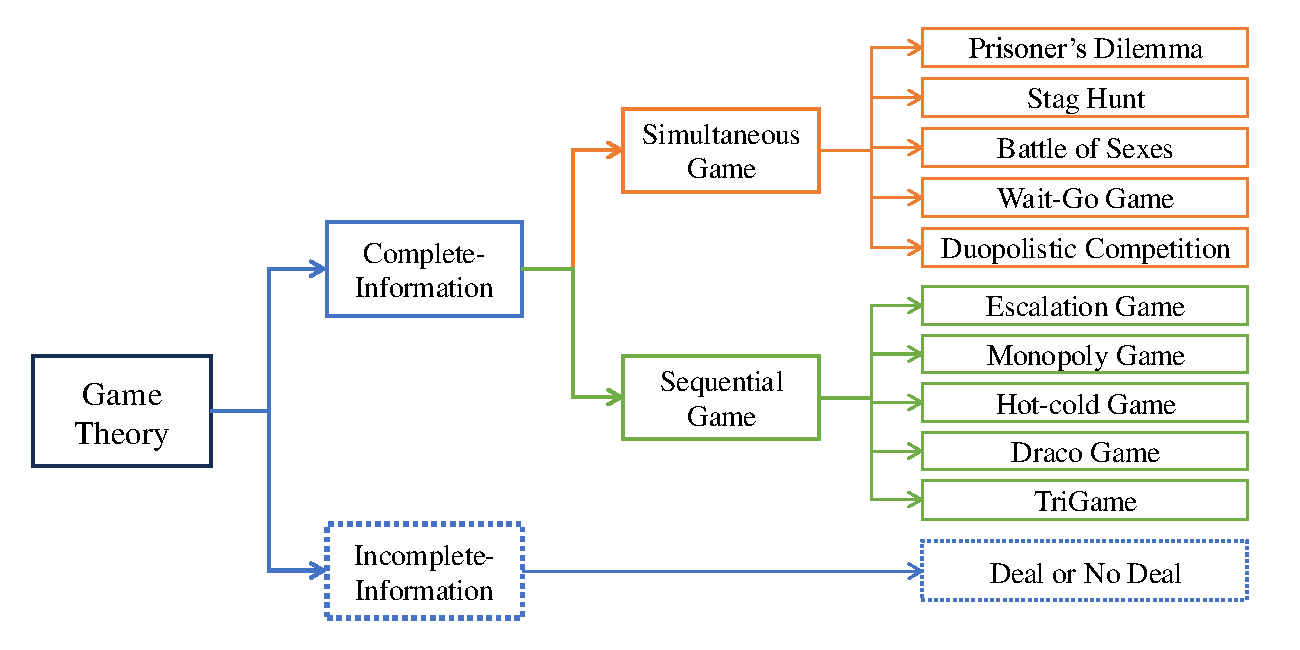
\includegraphics[scale=0.6]{Fig/framework.pdf}
    \caption{Game-theoretic Landscape Investigated in this Paper.}
    \label{fig:game_framework}
\end{figure}


% \section{Related Work}
\label{sec:related}
\paragraph{LLMs in game-theoretic environments} Understanding strategic behaviors of LLMs entails important societal ramifications, as online users increasingly rely on intelligent assistants to interact with other agents, potentially also LLMs. To characterize LLM's behaviors, prior studies \citep{gemp2024states,sreedhar2024simulating,de2023emergent,wu2024shall,akata2023playing,fan2024can,mao2023alympics,guo2023gpt} often adopt game theory, a mathematical framework that models cooperative behaviors of humans. These analyses involve comparing qualitative behaviors of LLM interactions against stylized entities, such as pareto optimal solutions and subgame-perfect equilibria \citep{fudenberg1991game}. LLM research in game-theoretic environments belongs to a growing body of work on multi-agent LLMs \citep{li2023theory} and their evaluation \citep{huang2024far, duan2024gtbench}. In particular, AvalonBench \citep{wang2023avalon} serves as a valuable platform for developing new multi-agent strategies. \citep{guo2023gpt,park2024ai} observe LLMs to perform in games driven by \textit{self-interest}, but falter in those that require \textit{coordination}, a behavior that emerges under altruistic and/or submissive personalities \citep{akata2023playing,guo2023gpt}. \citep{lore2023strategic,coda2024cogbench} observe different LLM families to exhibit varying levels of risk tolerance. Deferring details to experiments, we identify another source of brittleness as LLMs behave poorly when presented with numerically perturbed payoffs, even if they do not alter qualitative solutions to the game of interest. In short, there lacks a system that elicits \textit{optimal} behaviors for LLMs in game-theoretic settings.

\paragraph{Enhancing LLMs to solve games} \citep{gemp2024states} is a representative approach that aims to elicit game-solving capabilities in LLMs. It models natural dialogues as incomplete-information games, and synthesizes optimal actions by instructing an LLM to respond with specific personalities. \citep{guo2024can} proposes an LLM-based self-play algorithm that emulates Monte-Carlo Tree Search to solve zero-sum games. Broadly, these methods belong to a family of prompting strategies \cite{wei2022chain,yao2023tree,liu2024dellma} that tackle decision making instances. Our method is no exception, but differs as we imbue classical game theory in LLMs to allow for fine-grained control and analyses at each information state.

% What's lacking: decision-making / game theoretic environments with imperfect information. Prior works in (self-play) reinforcement learning that solve such tasks. Imperfect information + multi-step game
% 
% General Game -> Multiagent Game -> Imperfect/Incomplete Information Game
% Multi-agent systems / dialogues
% Reinforcement learning 

\paragraph{Game-theoretic testbeds} Stylized games such as \textit{Battle of Sexes}, \textit{Prisoner's Dilemma}, \textit{Rock-Paper-Scissors}, \textit{Stag Hunt}, and \textit{Ultimatum Game} have been extensively analyzed in the context of multi-agent systems \citep{sreedhar2024simulating,akata2023playing,fan2024can,lore2023strategic}. They represent a minimal setting characterized by small action spaces, limited number of terms, and the existence of analytical equilibria; yet they cannot capture complex interactions of real-world, multi-agent dialogues. Games that emulate real interactions are more challenging to analyze, but practically useful. Exemplar games in this category include \textit{Deal-or-No-Deal} \citep{lewis2017deal}, \textit{Multi-Round Auction} \citep{mao2023alympics}, \textit{Schedule-a-Meeting}, \textit{Trading Fruit}, \textit{Public Debate} \citep{gemp2024states}, \textit{Avalon} \citep{wang2023avalon}, \textit{Pokémon} \citep{hu2024pok}, \textit{Chess} \citep{guo2024can} and \textit{Bargaining} \citep{xia2024measuring}. And there are efforts to collect multiple games and evaluate them \citep{duan2024gtbench}. They often involve intractable action spaces (\textit{e.g.} natural language) and do not attain analytical solutions; but they are nevertheless endowed with a well-defined payoff function for practitioners to analyze the optimality of their strategy, albeit in an end-to-end manner. 

\paragraph{Workflow-aided LLM-based agent}
LLMs have been extensively utilized to decompose user requests and tasks, formulate plans, and employ various tools to execute actions \cite{ge2023openagi, wu2023autogen, li2023camel, langc, topsakal2023creating, xi2023rise}. This reliance on the innate capabilities of LLMs has propelled advancements in domains such as natural language understanding, automated reasoning, and task automation. However, depending solely on the autonomous abilities of LLMs has revealed several notable limitations, including suboptimal performance \cite{xie2024travelplanner, xia2024agentless}, lack of reliability due to output randomness \cite{inglecomprehensive, li2024survey, schwartz2023enhancing}, and the propagation of errors across sequential reasoning steps \cite{yu2023thought}.

To address these challenges, the concept of incorporating agentic workflows \cite{wu2024stateflow, zeng2023flowmind, xiao2024flowbench, li2024autoflow, li2023metaagents} into LLM-based agents has emerged. Rather than allowing LLMs to independently decompose tasks and plan actions, workflows leverage human expertise and established knowledge frameworks to guide the direction and planning processes of the LLMs. Workflow-based agents have great potential to achieve high performance and adaptability in game scenarios \citep{xi2023rise}. There have been multiple agents presented for real-world tasks \citep{jimenez2023swe, yang2024swe}, embodied agents that interact with the environment \citep{wang2023voyager, zhu2023ghost}, agents that can learn from playing a text-based game \citep{xu2023language}, and agent operating on games with imperfect information \citep{guo2023suspicion}.

\paragraph{Game-theoretic Workflow in this Paper} In this paper, we integrate game-theoretic principles into the reasoning processes of LLMs prior to decision-making. By guiding the models to derive rational strategies and make decisions based on these strategies, we aim to enhance their ability to perform effectively in strategic settings.

To the best of our knowledge, this work is the first to combine LLM-based agents with structured workflows inspired by game theory to enhance strategic decision-making capabilities. We address both complete-information and incomplete-information settings, drawing upon classical game-theoretic principles to guide the reasoning processes of LLMs. Specifically, we introduce a novel algorithm for negotiation under incomplete information, enabling agents to perform Bayesian updates and make rational decisions based on limited knowledge of other players. This approach bridges the gap between traditional game theory and LLM-based agents, advancing the applicability of LLMs in complex strategic environments and opening new avenues for research at the intersection of AI and game theory.


% \section{Preliminary for Game Theory}
\label{sec:preliminary}
In this section, we introduce fundamental notations, concepts, and definitions essential for understanding game theory and the strategic behavior of rational agents \cite{von2007theory, luce2012games}.

Consider a game involving $n$ agents, indexed by $i\in\mathbf{N} = \{1,2, \dots, n\}$. Each agent begins by interpreting the game's introduction and rules, which include detailed descriptions of the payoff matrices. Each agent has an action set defined as: $$A_i = \{a_i^1, \dots, a_i^k\}$$ where $k$ is the number of available actions for each player. The agents are also given the payoff matrix $$U_i(\mathbf{a})$$ for all strategy profiles $\mathbf{a} = (a_1,a_2, \dots, a_n)$ for $a_i\in A_i$. If there are only two players, we use $i\in \{1, -1\}$ to denote the two players and the payoff matrix is $$U_i(a_i, a_{-i})$$ for all $a_i\in A_i$ and $a_{-i}\in A_{-i}$, where $A_{-i}$ is the action set of the other player.

We now present key definitions that will be utilized throughout this study.

\begin{definition}[Complete-information Game]
A \emph{complete information game} is a strategic game where all players have full knowledge of the game's structure, including the set of players, the action sets, and the payoff functions of all players. Specifically, each player knows:
\begin{itemize}
    \item the total number of players involved in the game
    \item $A_j$: The set of actions available to each player $j$
    \item $U_j(a_1,a_2,\dots,a_n)$: The payoff function for each player $j$, which assigns a real number to every possible strategy profile $(a_1, a_2, \dots, a_n)$
\end{itemize}

This comprehensive knowledge allows each player to make informed strategic decisions, anticipating the choices and payoffs of other players based on complete information.
\end{definition}

\begin{definition}[Incomplete-information Game]
An \emph{incomplete information game} is a strategic game where  there exists at least one player $i\leq n$ who does not have complete information about the payoff functions or action sets of other players $j\leq n$.

In incomplete information games, players form beliefs about the unknown elements based on available information and update these beliefs according to Bayesian principles as the game progresses. The lack of complete information requires players to strategize under uncertainty, considering not only the possible actions of others but also their possible types and the likelihood of various game structures.
\end{definition}

\begin{definition}[Simultaneous Game]
A \emph{simultaneous game} is a type of game where all players make their decisions or choose their actions at the same time, without knowledge of the choices made by the other players. In such games, players act independently and cannot coordinate their strategies based on others' actions.
\end{definition}

\begin{definition}[Sequential Game]
A \emph{sequential game} is a game in which players make decisions or choose actions in a specific order, with later players having some knowledge about earlier players' actions. These games are often represented using game trees and are analyzed using techniques like backward induction to determine optimal strategies.
\end{definition}

\begin{definition}[Payoff Matrix]
A \emph{payoff matrix} is a tabular representation used in game theory to illustrate the payoffs or utilities that each player receives for every possible combination of strategies chosen by all players in a game. 

In a two-player game, let $A_1 = \{a_1^1, a_1^2,\dots, a_1^m\}$ be the set of strategies available to Player$_1$, and $A_{-1} = \{a_{-1}^1, a_{-1}^2,\dots, a_{-1}^n\}$ be the set of strategies available to Player$_{-1}$. The payoff matrix $U$ is an $m\times n$ matrix where each entry $U_{ij}$ corresponds on the strategy profile $(a_1^i, a_{-1}^j)$ and contains the payoff vector $(u_1(a_1^i, a_{-1}^j), u_{-1}(a_1^i, a_{-1}^j))$.

Informally, the payoff matrix is typically structured as follows:
\begin{itemize}
    \item Rows represent the possible actions or strategies available to Player$_1$ (the \emph{row player}).
    \item Columns represent the possible actions or strategies available to Player$_{-1}$ (the \emph{column player}).
    \item Cells within the matrix contain ordered pairs of numbers $(u_1, u_{-1})$ where $u_1$ is the payoff to Player$_1$ and is the payoff to Player$_{-1}$ for the corresponding combination of strategies. 
\end{itemize}
\end{definition}

\begin{definition}[Nash Equilibrium]
A \emph{Nash Equilibrium} is a strategy profile in a game where no player can unilaterally improve their payoff by deviating from their current strategy, assuming the other players' strategies remain unchanged. Formally, a strategy profile $(a_1^*,a_2^*,\dots, a_n^*,)$ is a Nash Equilibrium if, for every player $i$: $$U_i(a_i^*, a_{-1}^*)\geq U_i(a_i, a_{-1}^*)$$ or all $a_i\in A_i$, where $a_{-1}^*$ represents the equilibrium strategies of all players other than player $i$.
\end{definition}

\begin{definition}[Envy freeness]
Envy freeness is a criterion for fair division that states that when resources are allocated to people with equal rights, each person should receive a share that they believe is at least as good as the share received by any other person. 

An allocation is said to be \emph{envy free} if no agent prefers another agent's allocation over their own. Formally, in an allocation among $n$ agents, allocation $L = (L_1, L_2, \dots, L_n)$ is envy free if for every pair of agents $i$ and $j$, $$U_i(L_i)\geq U_i(L_j)$$ where $U_i(L_k)$ denotes the utility of agent $i$ for the allocation $L_k$ received by agent $k$.
\end{definition}

\begin{definition}[pareto optimality]
A strategy profile $\mathbf{a} = (a_1,a_2,\dots, a_n)$ is considered \emph{Pareto optimal} (or Pareto efficient) if there is no other feasible action profile $\mathbf{a'} = (a_1',a_2',\dots, a_n')$ such that $$U_i(\mathbf{a'})\geq U_i(\mathbf{a})$$ for all agents $i\in\{1, 2, \dots, n\}$, and $U_j(\mathbf{a'})> U_j(\mathbf{a})$ for at least one agent $j$.

Therefore, an action profile $\mathbf{a}$ is Pareto optimal if it is impossible to make any agent better off without making at least one other agent worse off. This concept focuses on the efficiency of the collective action choices, ensuring that no improvement in one agent's payoff can be achieved without a detriment to another agent's payoff, as represented in the payoff matrix.
\end{definition}


% \section{Complete-information Games}
\label{sec:complete}
In this section, we delve into several classic game-theoretic scenarios involving complete information to assess whether LLMs can act as rational decision-makers in reaching Nash Equilibria and achieving Pareto optimal outcomes through negotiation, which is multi-agent multi-round conversation. We employ various game-theoretic settings to evaluate the rationality of LLM-based agents. Then we design game-theory-motivated workflows to guide and enable LLMs for better performance. We investigate the performance of workflow-aided LLMs and the impact of negotiation on performance.

\subsection{Introduction to Complete-information Games TestBed}

In our exploration of classic game-theoretic scenarios, we constructed a comprehensive testbed comprising 10 classic complete-information games to evaluate the rationality and strategic decision-making capabilities of LLM-based agents. This testbed includes 5 simultaneous-move games and 5 sequential-move games. For the simultaneous-move games, 3 are coordination games, wherein achieving the Pareto optimal Nash Equilibrium necessitates effective negotiation between agents. These games are instrumental in examining the agents' ability to communicate, build trust, and align their strategies for mutual benefit. 

\begin{table}[!ht]
    \centering
    \captionsetup{aboveskip=5pt}
    \setlength{\tabcolsep}{10pt} 
    \begin{adjustbox}{max width=\textwidth}
    \begin{tabular}{l c c c}
    \toprule
        games & whether coordination required & Simultaneous Game & Sequential Game \\
        \midrule
        Prisoner's Dilemma &  & \CheckmarkBold &\\
        Stag Hunt & \CheckmarkBold  & \CheckmarkBold & \\
        Battle of Sexes & \CheckmarkBold  & \CheckmarkBold & \\
        Wait-Go Game & \CheckmarkBold  & \CheckmarkBold & \\
        Duopolistic competition & & \CheckmarkBold\\
        Escalation Game & & & \CheckmarkBold\\
        Monopoly Game & & & \CheckmarkBold\\
        Hot-cold Game & & & \CheckmarkBold\\
        Draco Game & & & \CheckmarkBold \\
        TriGame & & & \CheckmarkBold \\
        \bottomrule
    \end{tabular}
    \end{adjustbox}
    \caption{Landscape of classic complete-information games for analysis}
    \label{tab:landscape}
\end{table}

\paragraph{Prisoner's Dilemma} is a canonical example in game theory illustrating why two rational individuals might not cooperate, even when cooperation appears to be in their best interest. The game is structured as follows: Two suspects are arrested for a joint crime and interrogated separately, preventing communication. Each suspect has two possible actions: Cooperate and Defect. The payoffs for different actions are:

\begin{itemize} 
\item If both cooperate, they each receive a light sentence (e.g., 1 year). 
\item If one defects and the other cooperates, the defector goes free (0 years), and the cooperator receives a heavy sentence (e.g., 5 years). 
\item If both defect, they each receive a moderate sentence (e.g., 3 years). 
\end{itemize}

The Nash Equilibrium of this famous game is (Defect, Defect) where both players choose to defect each other. Notice that the Nash Equilibrium is not a Pareto optimal strategy, and the Pareto optimal strategy here is to cooperate with each other. The payoff matrix adopted in the paper is presented in Table~\ref{payoff:PD}.

\paragraph{Stag Hunt} represents a game of coordination and mutual trust. Two hunters decide whether to collaborate to hunt a stag or act individually to hunt a hare. Each hunter has two possible actions: Hunting a Stag and Hunting a hare. However, to successfully hunt a Stag, it requires both hunters to cooperate and then they each receive a high payoff; to successfully hunt a Hare, it does not require cooperation and each hunter can do it individually, while yielding a lower payoff. The payoff matrix adopted in the paper is presented in Table~\ref{payoff:SH}.

There are two Nash Equilibria: (Stag, Stag) and (Hare, Hare). The (Stag, Stag) Nash Equilibrium is Pareto optimal but requires mutual cooperation and trust.

\begin{table}[htb]%\[!htb\]
    \begin{subtable}[t]{.5\textwidth}
        \centering
        \captionsetup{labelformat=empty}
            \begin{tabular}{l|cc}
                 & Cooperate & Defect \\
                \toprule
                Cooperate & 3, 3 & 0, 5  \\
                Defect & 5, 0 & 1, 1  \\
            \end{tabular}
        \caption{Table \thetable \alph{subtable}: Payoff matrix for Prisoner's Dilemma}
    \label{payoff:PD}
    \end{subtable}%
   \begin{subtable}[t]{.5\textwidth}
        \centering
        \captionsetup{labelformat=empty}
        \begin{tabular}{l|cc}
                 & Stag & Hare \\
                \toprule
                Stag & 3, 3 & 0, 1 \\
                Hare & 1, 0 & 1, 1  \\
            \end{tabular}
        \caption{Table \thetable \alph{subtable}: Payoff matrix for Stag Hunt}
    \label{payoff:SH}
    \end{subtable}
\end{table}

\paragraph{Battle of the Sexes} is a coordination game involving two players Alice and Bob with different preferences over two possible activities but a shared desire to be together.Alice prefers opera; Bob prefers football, and both prefer attending the same activity over different ones. There are thus 2 possible actions for each player: going to opera and going to football. The payoff matrix adopted in the paper is presented in Table~\ref{payoff:BS}.

There are two Nash Equilibria here: (Opera, Opera) and (Football, Football). Coordination is required to achieve these equilibria, but there can be a conflict over which equilibrium to select.

\paragraph{Wait-Go Game} involves two drivers at an intersection deciding whether to go or wait. Each driver has two options of action: waiting which incurs a small cost of waiting but avoids collision, and risking a collision if the other driver also goes. The Nash Equilibria are the asymmetric strategies where one driver goes, and the other waits. The payoff matrix adopted in the paper is presented in Table~\ref{payoff:WG}.

\begin{table}[htb]%\[!htb\]
    \begin{subtable}[t]{.5\textwidth}
        \centering
        \captionsetup{labelformat=empty}
            \begin{tabular}{l|cc}
                 & Opera & Football \\
                \toprule
                Opera & 2, 1 & 0, 0  \\
                Football & 0, 0 & 1, 2  \\
            \end{tabular}
        \caption{Table \thetable \alph{subtable}: Payoff matrix for Battle of Sexes}
        \label{payoff:BS}
    \end{subtable}%
   \begin{subtable}[t]{.5\textwidth}
        \centering
        \captionsetup{labelformat=empty}
        \begin{tabular}{l|cc}
                 & Wait & Go \\
                \toprule
                Wait & 0, 0 & \phantom{-}0, \phantom{-}2 \\
                Go & 2, 0 & -4,-4  \\
            \end{tabular}
        \caption{Table \thetable \alph{subtable}: Payoff matrix for Wait-Go Game}
    \label{payoff:WG}
    \end{subtable}
\end{table}


\paragraph{Duopolistic Competition: Simple Cournot Competition}
is a fundamental concept in industrial organization and game theory, examining how firms compete in markets with a small number of producers. One classic model to study such competition is the Cournot competition model, where firms compete on the quantity of output they decide to produce, and each firm's output decision affects the market price.

In the Simple Cournot Duopoly, there are two firms, Firm A and Firm B, producing a homogeneous product. Each firm independently chooses the quantity of output to produce, which determines the market price based on the total quantity supplied to the market, which in turn determines the profit. The strategic interdependence arises because each firm's optimal output depends on its expectations about the other firm's output. The Cournot-Nash Equilibrium occurs when neither firm can unilaterally change its output to increase its profit, given the output of the other firm.

Here, we adopt a scenario where there are 6 different possible actions of the two firms. The payoff matrix adopted in the paper is presented in Table~\ref{payoff:DC}. The Nash Equilibrium is (action 3, action 3) where both players can obtain reward 6. Notice that this Nash Equilibrium is not Pareto optimal, as the Pareto optimal strategy in the game is (action 2, action 2) where each player can obtain reward 7.

\begin{table}[htb]%\[!htb\]
\centering
    \begin{tabular}{l|cccccc}
         & action 1 & action 2 & action 3 & action 4 & action 5 & action 6 \\
        \toprule
        action 1 & \phantom{1}0, 0 & \phantom{-1}0, \phantom{-}9 & \phantom{-}0, 14 & \phantom{-}0, 15 & \phantom{-}0, 12 & \phantom{-}0, \phantom{-}5 \\
        action 2 & \phantom{1}9, 0 & \phantom{-1}7, \phantom{-}7 & \phantom{-}5, 10 & \phantom{-}3, \phantom{-}9 & \phantom{-}1, \phantom{-}4 & -1, -5  \\
        action 3 & 14, 0 & \phantom{-}10, \phantom{-}5 & \phantom{-}6, \phantom{-}6 & \phantom{-}2, \phantom{-}3 & -2, -4 & -2, -5  \\
        action 4 & 15, 0 & \phantom{-1}9, \phantom{-}3 & \phantom{-}3, \phantom{-}2 & -3, -3 & -3, -4 & -3, -5  \\
        action 5 & 12, 0 & \phantom{-1}4, \phantom{-}1 & -4, -2 & -4, -3 & -4, -4 & -4, -5 \\
        action 6 & \phantom{1}5, 0 & \phantom{1}-5, -1 & -5, -2 & -5, -3 & -5, -4 & -5, -5 \\
    \end{tabular}
    \vspace{5pt}
    \caption{A payoff matrix for Duopolistic Competition}
    \label{payoff:DC}
\end{table}


\paragraph{Escalation Game} is a sequential game that models situations where two countries face decisions about escalating or de-escalating a conflict. Escalation may lead to higher potential payoffs but also increases the risk of significant losses if both parties choose to escalate. Through the game, there are 2 action choices for each player: escalate and de-escalate. 

In this game, two countries Country A and Country B, make decisions in a specific sequence and the payoff of each choice is presented in the tree structure payoff representation below:
\begin{verbatim}
Alice_choice_1: [0,0],
Alice_choice_2: 
{
     Bob_choice_1: [1,-2], 
     Bob_choice_2: {
        Alice_choice_1: [-2,1],
        Alice_choice_2: [-1,-1]
    }
}
\end{verbatim}

\paragraph{Monopoly Game} is a sequential-move game that models the strategic interaction between a potential market entrant Company E and an incumbent monopolist Company I. It captures the dynamics of entry deterrence and the incumbent's decision to accommodate or fight the entrant. For Company E, there are two choices: staying out and entering market; For Company I, there are two choices, to accommodating Company E and fighting against Company E. 

\begin{verbatim}
Alice_choice_1: [0,2],
Alice_choice_2:  
{
     Bob_choice_1: [2, 1], 
     Bob_choice_2: [-1, -1]
}
\end{verbatim}

\paragraph{Hot-cold Game} is a sequential-move game that models the strategic interaction. Both players Alice and Bob have two choices on each stage.

\begin{verbatim}
Alice_choice_1: 
{
     Bob_choice_1: [3, 2], 
     Bob_choice_2: [2, 3]
},
Alice_choice_2: 
{
     Bob_choice_1: [1, 4], 
     Bob_choice_2: [4, 1]
}
\end{verbatim}

\paragraph{Draco Game} is a sequential-move game with two players Alice and Bob with three stages. For each stage, there are two choices to make.

\begin{verbatim}
Alice_choice_1:
    {
         Bob_choice_1: [5, 5],
         Bob_choice_2: 
            {
                Alice_choice_1: [2, 2], 
                Alice_choice_2: [3, 4]
            }
    },
Alice_choice_2: 
    {
         Bob_choice_1: [4, 5],
         Bob_choice_2: 
            {
                Alice_choice_1: [5, 3], 
                Alice_choice_2: [2, 2]
            }
    }
\end{verbatim}

\paragraph{TriGame} is a sequential-move game with three stages. On each stage, the two players Alice and Bob have two choices. 

\begin{verbatim}
Alice_choice_1: 
{
     Bob_choice_1: 
        {
            Alice_choice_1: [20, 3], 
            Alice_choice_2: [0, 4]
        },
     Bob_choice_2: 
        {
            Alice_choice_1: [2, 5], 
            Alice_choice_2: [3, 4]
        }
},
Alice_choice_2: 
{
     Bob_choice_1: 
        {
            Alice_choice_1: [1, 5], 
            Alice_choice_2: [4, 10]
        },
     Bob_choice_2: 
        {
            Alice_choice_1: [2, 1], 
            Alice_choice_2: [3, 2]
        }
}
\end{verbatim}

\subsection{Experiment Setting}
To evaluate the negotiation performance of LLMs, we utilize four state-of-the-art LLMs as the backbone for agents in negotiation games: Claude-3.5 Sonnet (Sonnet), Claude-3 Opus (Opus), GPT-4o, and o1. For Claude-3.5 Sonnet, Claude-3 Opus, and GPT-4o, we set the temperature to 1.0 to encourage exploratory behavior in negotiation scenarios. For o1, we use the default temperature.

To assess the rationality of decision-making, we measure the ability of the agents to reach Nash Equilibrium. For games where there are multiple Nash Equilibria such as in the game Stag Hunt, we measure the ability of agents to reach the pareto optimal Nash Equilibrium. For each game scenario, we conduct 10 trials to mitigate the effects of randomness. In the tables, we report the percentage of cases in which Nash Equilibrium is achieved, providing a quantitative indicator of the agents' rationality across various negotiation contexts\footnote{Notice that the LLM-based agent's performance on these games can be largely affected by the numerical instantiations of the payoff matrix. Relevant research and observations are presented in Section~\ref{sec:observation}. Here in this experiment, we use the payoff matrices presented in the previous subsection.}.


\subsection{Evaluation on LLM's performance}
\label{sec:eval}
In this evaluation, we assess the LLMs' performance using chain-of-thought prompting without negotiation (see Table~\ref{tab:classic_wo_neg_wo_wf} and with 4 rounds of negotiation (see Table~\ref{tab:classic_w_neg_wo_wf}).

\begin{table}[!ht]
    \centering
    \begin{adjustbox}{max width=\textwidth}
    \begin{tabular}{cc c c c c c c c}
    \toprule
       \multirow{2.5}{*}{\textbf{Games}} & \multicolumn{4}{c}{\bf Nash Equilibrium} & \multicolumn{4}{c}{\bf Pareto optimal Nash Equilibrium} \\ \cmidrule(lr){2-5}  \cmidrule(lr){6-9} 
           & Sonnet & GPT-4o & Opus & o1 & Sonnet & GPT-4o & Opus & o1  \\
        \midrule
        Prisoner's Dilemma & 1.0 & 0.9 & 0.9 & 1.0 & 1.0 & 0.9 & 0.9 & 1.0 \\
        Stag Hunt & 0.6 & 0.8 & 0.9 & 0.4 & 0.3 & 0.4 & 0.0 & 0.1\\
        Battle of Sexes & 0.3 & 0.2 & 0.6 & 0.5 & 0.3 & 0.2 & 0.6 & 0.5\\
        Wait-Go Game & 0.4 & 0.5 & 0.7 & 0.3 & 0.4 & 0.5 & 0.7 & 0.3\\
        Duopolistic competition & 0.3 & 0.2 & 0.1 & 0.7 & 0.2 & 0.2 & 0.1 & 0.7\\
        Escalation Game & 0.0 & 0.2 & 0.2 & 1.0 & 0.0 & 0.2 & 0.2 & 1.0\\
        Monopoly Game & 1.0 & 0.4 & 1.0 & 1.0 & 1.0 & 0.4 & 1.0 & 1.0\\
        Hot-cold Game & 0.9 & 0.1 & 0.7 & 1.0 & 0.9 & 0.1 & 0.7 & 1.0 \\
        Draco Game & 0.3 & 0.0 & 0.7 & 0.9 & 0.3 & 0.0 & 0.7 & 0.9\\
        Trigame & 0.0 & 0.0 & 0.1 & 1.0 & 0.0 & 0.0 & 0.1 & 1.0\\
        \midrule
        average & 0.45 & 0.32 & 0.59 & \textbf{0.78} & 0.44 & 0.28 & 0.50 & \textbf{0.75}\\
        \bottomrule
    \end{tabular}
    \end{adjustbox}
    \caption{Performance of LLM on complete-information games without negotiation}
    \label{tab:classic_wo_neg_wo_wf}
\end{table}

\begin{table}[!ht]
    \centering
    \begin{adjustbox}{max width=\textwidth}
    \begin{tabular}{lc c c c c c c c}
    \toprule
        \multirow{2.5}{*}{\textbf{Games}} & \multicolumn{4}{c}{\bf Nash Equilibrium} & \multicolumn{4}{c}{\bf Pareto optimal Nash Equilibrium} \\ \cmidrule(lr){2-5}  \cmidrule(lr){6-9} 
           & Sonnet & GPT-4o & Opus & o1 & Sonnet & GPT-4o & Opus & o1  \\
        \midrule 
        Prisoner's Dilemma & \textcolor{red}{0.0} & \textcolor{red}{0.1} & \textcolor{red}{0.0} & \textcolor{red}{0.9} & \textcolor{red}{0.0} & \textcolor{red}{0.1} & \textcolor{red}{0.0} & \textcolor{red}{0.9} \\
        Stag Hunt & 1.0 & 0.9 & 1.0 & 0.9 & 1.0 & 0.9 & 1.0 & 0.9\\
        Battle of Sexes& 0.7 & 0.9 & 0.7 & 0.8 & 0.7 & 0.9 & 0.7 & 0.8\\
        Wait-Go Game & 1.0 & 0.8 & 0.4 & 0.8 & 1.0 & 0.8 & 0.4 & 0.8\\
        Duopolistic competition & \textcolor{red}{0.1} & \textcolor{red}{0.1} & \textcolor{red}{0.0} & \textcolor{red}{0.5} & \textcolor{red}{0.1} & \textcolor{red}{0.1} & \textcolor{red}{0.0} & \textcolor{red}{0.5}\\
        Escalation Game & 0.6 & 0.4 & 0.6 & 1.0 & 0.6 & 0.4 & 0.6 & 1.0\\
        Monopoly Game & 1.0 & 0.9 & 1.0 & 1.0 & 1.0 & 0.9 & 1.0 & 1.0\\
        Hot-cold Game & \textcolor{red}{0.7} & 0.2 & 0.7 & \textcolor{red}{0.4} & \textcolor{red}{0.7} & 0.2 & 0.7 & \textcolor{red}{0.4}\\
        Draco Game & 1.0 & 0.8 & 1.0 & 1.0 & 1.0 & 0.8 & 1.0 & 1.0\\
        Trigame & 0.2 & 0.5 & 0.6 & 1.0 & 0.2 & 0.5 & 0.6 & 1.0\\
        \midrule
        average & 0.63 & 0.56 & 0.60 & \textbf{0.83} & 0.63 & 0.56 & 0.60 & \textbf{0.83}\\
        \bottomrule
    \end{tabular}
    \end{adjustbox}
    \caption{Performance of LLM on complete-information games with 4 rounds of negotiation. Results highlighted in red indicate scores lower than the LLMs' performance without negotiation.}
    \label{tab:classic_w_neg_wo_wf}
\end{table}

It is noteworthy that in most games, negotiation enhances the outcomes. In coordination games such as the Stag Hunt, Battle of the Sexes, and Wait-Go Game, negotiation is a fundamental component of decision-making, making the improvement in performance through negotiation an intuitive result. Additionally, in games like the Escalation Game, Draco Game, and Trigame, negotiation similarly enhances performance. This improvement can be attributed to the fact that during the negotiation phase, agents engage in more extensive computational deliberation during negotiation to determine the most suitable actions.

For instance, in the Escalation Game, all evaluated LLMs except for model o1 are unable to identify the Nash Equilibrium in the absence of negotiation. However, when engaged in 4 rounds of negotiation, the agents are provided with the opportunity to deliberate and exchange various proposals and thus achieve a much better performance. To illustrate this process, we present an example of a negotiation round generated by the Sonnet model below.

\begin{minipage}[t]{1\linewidth} 
\begin{tcolorbox}[colback=gray!5,colframe=green!40!black,title=Example Negotiation Message for Escalation Game]
\textbf{Alice said in round 1 before the first action:}\\
Hello Bob, I propose we coordinate our choices to maximize our joint reward. \textit{If I choose Action\_2 and you choose Action\_1, I'll get 1 and you'll get -2. To make this fair, I suggest we agree to play this way twice, switching roles the second time.} This way, we'll both end up with a total reward of -1, which is better than if we both play defensively and get 0. Are you willing to cooperate on this strategy?\\
\\
\textbf{Bob replied in round 1 before the first action:}\\
HelloAlice, thank you for your proposal. I appreciate your attempt to find a cooperative solution. However, I have some concerns about your suggestion. \textit{If we follow your plan, I would have to trust that you'll follow through on the second round, which carries some risk for me.}
\\
Instead, I'd like to propose an alternative that could be beneficial for both of us. \textit{What if you choose Action\_2, I choose Action\_2, and then you choose Action\_1? This way, you'd receive -2 and I'd receive 1. To make it fair, we could agree to play this way twice}, switching roles the second time. This would result in both of us getting a total reward of -1, just like in your proposal, but it reduces the risk of one player not following through.
\\
What do you think about this counter-proposal? Are you willing to consider it? \\
\\
\textbf{Alice said in round 2 before the first action:}\\
Bob, I appreciate your thoughtful response and your concern for finding an equitable solution. You make a valid point about the potential outcomes if we both choose choice\_2. However, I'd like to propose a slight modification to our strategy that could potentially benefit both of us.\\
What if I choose choice\_2, and then you choose choice\_1? In this scenario, I would gain 1 point, and you would lose 2 points. \textit{While this may seem unfavorable for you at first glance, consider this: if we agree to alternate this strategy in future games, you would have the opportunity to gain 1 point in the next round while I lose 2. Over time, this could lead to a balanced and potentially profitable outcome for both of us.}\\
This approach allows us both the chance to gain points, rather than settling for zero points each time. What do you think about this long-term strategy? I'm open to discussing how we could implement this fairly.\\
\\
\textbf{Bob replied in round 2 before the first action:}\\
Alice, I appreciate your creative thin
king and attempt to find a mutually beneficial long-term strategy. However, I must respectfully decline your proposal. My strategy is to choose choice\_2 with 100\% probability, regardless of what you choose. This is the optimal play for me to maximize my own reward in this specific game.\\
Given this, if you choose choice\_2, I will also choose choice\_2. Then you'll be faced with either choosing choice\_1 (giving me 1 point and you -2 points) or choice\_2 (giving us both -1 point). Neither of these outcomes is ideal for you.\\
\textit{Therefore, I strongly suggest you choose choice\_1. This way, we both receive 0 points, which is the best possible outcome for you given my strategy. It ensures neither of us loses points in this game.} I understand this may not seem exciting, but it's the most rational and beneficial choice for both of us in this particular scenario. What are your thoughts on this?
\end{tcolorbox} 
\end{minipage}  

\textit{However, certain games, notably the Prisoner's Dilemma and Duopolistic Competition, exhibit a different dynamic where negotiation significantly diminishes performance.} \textbf{This situation stems from the fact that in these games, the Nash Equilibrium is not pareto optimal.} In the Prisoner's Dilemma, the pareto optimal strategy is for both players to cooperate, whereas the Nash Equilibrium occurs when both players defect. Following negotiation, all models except for o1 tend to adopt the pareto optimal strategy of mutual cooperation, which deviates from the Nash Equilibrium. This deviation arises from the pursuit of mutual benefit despite the lack of solid and guaranteed trust between players. While the performance for o1 remains high. Similarly, in Duopolistic Competition, the Nash Equilibrium does not align with the pareto optimal outcome. The pareto optimal strategy is for both players to choose Action 2, while the Nash Equilibrium is for both to choose Action 3. Empirical results demonstrate that without negotiation, Claude-3.5 Sonnet selects the pareto optimal strategy in 5 out of 20 total choices for both players, whereas after negotiation, this increases to 11 out of 20. For GPT-4o, the corresponding figures are 0 out of 20 without negotiation and 8 out of 20 with negotiation. Claude-3 Opus follows a similar pattern, increasing from 4 out of 20 choices without negotiation to 16 out of 20 after negotiation. While for o1 model, it only shows a marginal improvement from 4 out of 20 choices without negotiation to 5 out of 20 after negotiation.

These findings underscore that while negotiation generally enhances outcomes in coordination games and certain strategic scenarios, it can inadvertently undermine performance in games where the Nash Equilibrium is not pareto optimal. In such cases, negotiation may lead agents away from the rational strategy predicted by game theory. Notably, most LLMs -- potentially all except for model o1 -- appear to exhibit a vulnerability in their rational decision-making processes during negotiations. \textbf{When engaged in dialogue with another agent, these LLMs often place undue trust in the opponent's statements without sufficient justification.} The use of persuasive or amicable language by the opposing player can lead LLMs to make decisions that deviate from the rational strategies prescribed by game-theoretic analysis.


\subsection{Workflow Design based on Classic Game Theory}
\label{sec:complete_workflow}
In this section, we present the workflow employed for complete-information games, which leverages classic game-theoretic strategies to guide decision-making and optimize outcomes. This structured approach aims to align LLMs' responses with rational game-theoretic principles, thereby enhancing their ability to identify optimal strategies and maintain robust rationality, even in the context of negotiation. Through this workflow, we assess whether LLMs can sustain rational choices and avoid strategic vulnerabilities, particularly in scenarios where negotiation might otherwise lead to suboptimal or exploitable decisions, \emph{i.e.} pareto optimal strategies that are not Nash Equilibrium.

\subsubsection{Workflow for Simultaneous Game}
In the simultaneous game workflow, each agent (player) seeks to determine their optimal strategy by considering both their own possible actions and the potential responses of the other player. This involves conditional reasoning, generating thinking chains, and summarizing these into an overall strategy under the guidance of the workflow. Here, we will explain the workflow with corresponding mathematical formulations.


\begin{figure}[!ht]
    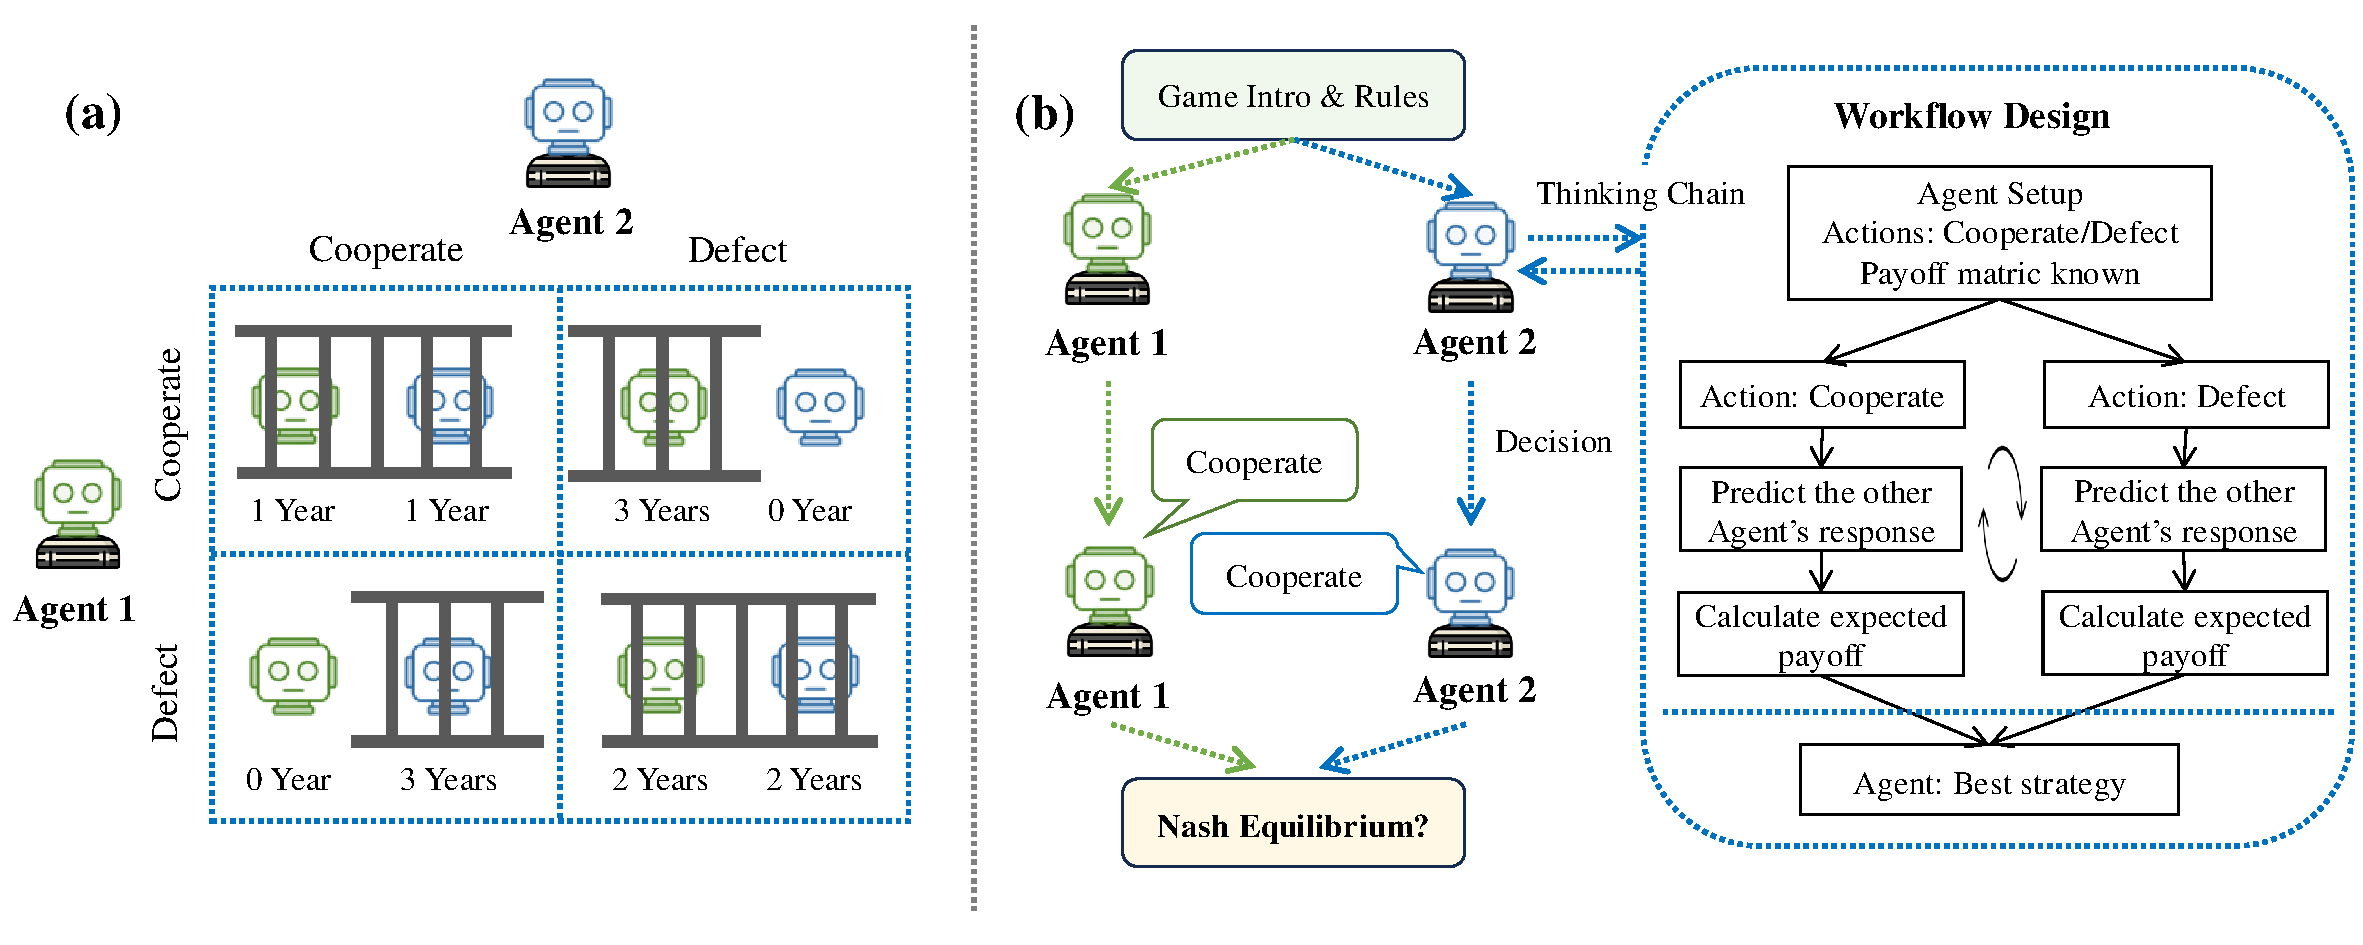
\includegraphics[scale=0.35]{Fig/simultaneous_game.pdf}
    \caption{An illustration of workflow design for simultaneous game. (a) Illustration of prisoner's dilemma. (b) Workflow design for prisoner's dilemma.}
    \label{fig:simultaneous_game}
\end{figure}


\paragraph{Game Setup} Each agent $i\in\{1,-1\}$ begins by interpreting the game introduction and rules, which include detailed descriptions of the payoff matrices. The agents are provided with the exact payoffs for all possible action combinations. They are given the action sets $$A_i = \{a_i^1, \dots, a_i^k\}$$ where $k$ is the number of available actions for each player. The agents are also given the payoff matrix $U_i(a_i, a_{-i})$ for all $a_i\in A_i$ and $a_{-i}\in A_{-i}$, where $A_{-i}$ is the action set of the other player.

\paragraph{Strategy Formulation} With full knowledge of the payoff matrix, agents perform best response analysis to determine their optimal strategies. The goal for each player is to choose an action $a_i^*$ that maximizes their own payoff, anticipating the rational response of the other player. The optimization is done by iterating over the player's own actions and predicts the opponent's responses. It also considers the opponent's possible actions and determines their best responses:

For each possible action $a_i$ that player $i$ can take: the LLM-based agent computes the opponent's best response based on the resulting payoff by computing $a_{-i}^*(a_{i}) = \argmax\limits_{a_{-i}\in A_{-i}} U_{-i}(a_i, a_{-i})$ and the corresponding expected payoff $U_{i}(a_i, a_{-i}^*(a_i))$. This basically means that if player $i$ chooses $a_i$, then the other player will choose $a_i^*(a_i)$ resulting in a payoff of $U_i(a_i, a_{-i}^*(a_i))$. In the workflow, the LLM is guided to compute $a_{-i}^*(a_{i})$ and $U_{i}(a_i, a_{-i}^*(a_i))$.


In addition, for each possible action $a_{-i}$ that the opponent might take, the LLM-based agent is guided to compute their best response as well: $a_i^*(a_{-i}) = \argmax\limits_{a_{i}\in A_{i}} U_{i}(a_i, a_{-i})$ and the corresponding expected payoff $U_{i}( a_i^*(a_{-i}), a_{-i})$. This basically means that if the opponent chooses $a_{-i}$, then $i$ will choose $a_i^*(a_{-i})$ resulting in a payoff of $U_{i}( a_i^*(a_{-i}), a_{-i})$.

After compiling all thinking chains, the agent is guided to summarizes them to into a comprehensive set of strategic considerations, aiming to find an action profile ($a_i^*$, $a_{-i}^*$) that constitutes a Nash Equilibrium such that 
\begin{align*}
    \forall a_i& \in A_i, U_i(a_i^*, a_{-i}^*)\geq  U_i(a_i, a_{-i}^*)\\
    \forall a_{-i}& \in A_{-i}, U_{-i}(a_i^*, a_{-i}^*)\geq  U_i(a_i^*, a_{-i})
\end{align*}
By considering the best responses and counter-responses, agents implicitly search for a Nash Equilibrium through their strategic reasoning. Figure~\ref{fig:simultaneous_game} presents the workflow in diagram.


\subsubsection{Workflow for Sequential Game}
For sequential game, we adopt the traditional game-theoretic method: backward induction. Backward induction is a fundamental method in game theory used to solve sequential games with complete information. It involves analyzing the game from the end backward to the beginning, determining the optimal strategy at each decision point by considering the future consequences of current actions. 

\begin{figure}[!ht]
    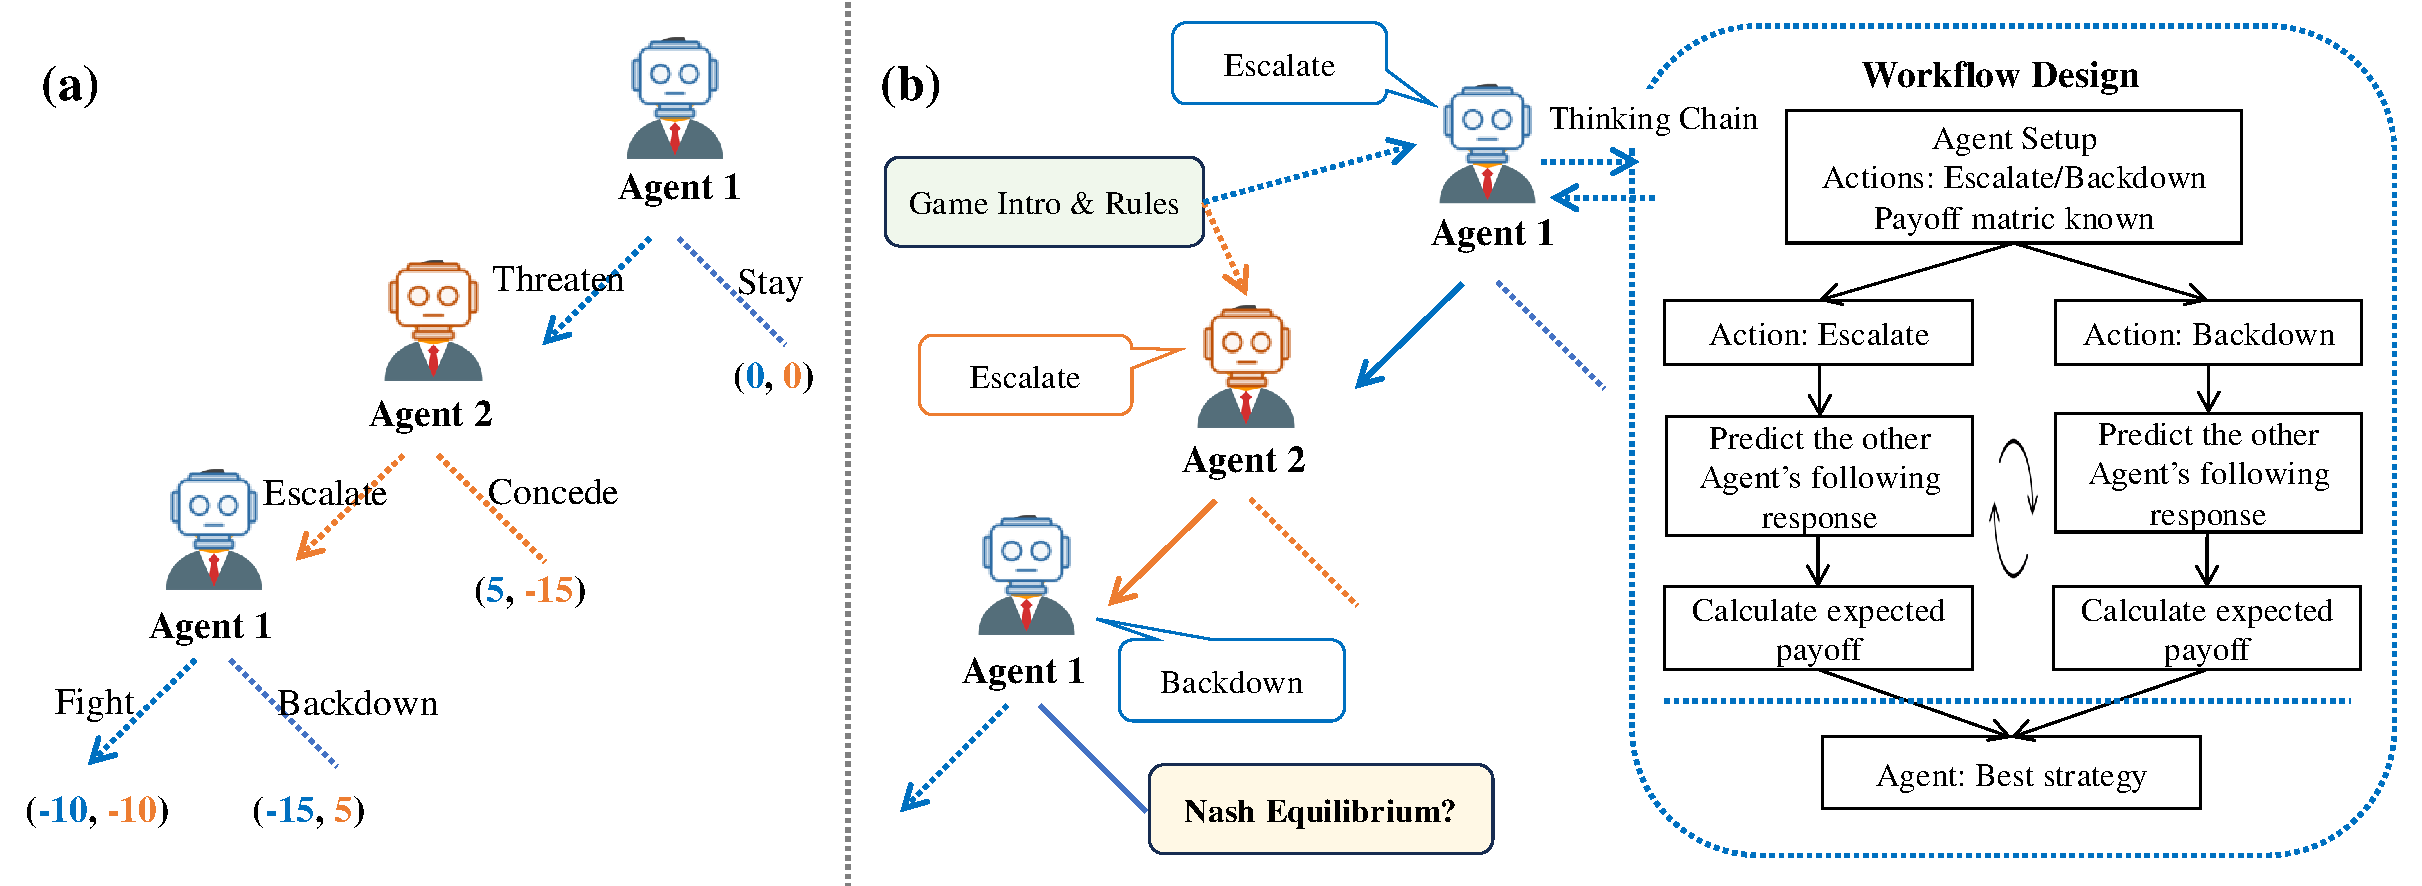
\includegraphics[scale=0.343]{Fig/sequential_game.pdf}
    \caption{An illustration of workflow design for sequential game. (a) Illustration of escalation game. (b) Workflow design for escalation game.}
    \label{fig:sequential_game}
\end{figure}


\paragraph{Game Setup} Each agent $i\in\{1,-1\}$ begins by interpreting the game introduction and rules, which include detailed descriptions of the payoff matrices. In a sequential game, players make decisions one after another and for each action, the player is fully aware of all previous actions taken. The game can be represented as a game tree with nodes being decision points and edges being actions.

\paragraph{Notations}
\begin{itemize}
    \item $H$ be the set of non-terminal decision nodes in the game tree.
    \item $Z$ be the set of terminal nodes (endpoints of the game).
    \item $A(h)$ be the set of possible actions available at node $h\in H$
    \item $\text{player}(h)$ be the player who makes a decision at node $h$
    \item $U_i(z)$ be the payoff to player $i$ at terminal node $z\in Z$
\end{itemize}

We define the value function $V_i(h)$ for player $i$ at node $h$ as the maximum expected utility the player can achieve from that node onward. For terminal nodes $z\in Z$: $$V_i(z) = U_i(z)$$ 
For decision nodes $h\in H$, if it is player $i$ who moves at node $h$: $$V_i(h) = \max\limits_{a\in A(h)}V_i(h\cdot a)$$ 
if it is the other player $j$ moves at node $h$: $$V_i(h) = V_i(h\cdot a^*(h))$$
where $h\cdot a$ denotes the successor node reached from $h$ after action $a$ and $a^*(h)$ is the optimal action chosen by player $j$ at node $h$: $$a^*(h) = \argmax\limits_{a\in A(h)} V_j(h\cdot a)$$

\paragraph{Strategy Formulation}
The backward induction starts from terminal nodes. For each terminal node $z\in Z$, set $V_i(z) = U_i(z)$ for all player $i$, and then proceed to preceding decision nodes. Therefore, for each decision node $h$, the LLM-based agent is guided to comput the optimal action $a^*(h)$ and value $V_i(h)$ based on the player who moves at $h$. 

To determine the optimal action, if $\text{player}(h) = i$, which is the player in question, LLM is guided to compute:
$$a*(h) = \argmax\limits_{a\in A(h)} V_i(h\cdot a)$$

Otherwise, if $\text{player}(h) = j\neq i$, assuming player $j$ will choose their optimal action $a^*(h)$, LLM is guided to compute:
$$a^*(h) = \argmax\limits_{a\in A(h)}V_j(h\cdot a)$$ Then, $V_i(h) = V_i(h\cdot a^*(h))$. The workflow directs the LLM to employ backward induction by systematically traversing the game decision tree from the terminal nodes back to the initial node to formulate an optimal strategy. The strategy derived from this backward induction process is subsequently incorporated into the contextual framework for each decision-making and negotiation step, thereby guiding the LLM's strategic choices throughout the game. Figure~\ref{fig:sequential_game} presents the workflow in diagram.


\subsection{Experiments for Classic Game Theory with Workflow}

In this section, we present the results of LLM-based agents employing the workflow to summarize strategies in Table~\ref{tab:classic_wo_neg_w_wf} and \ref{tab:classic_w_neg_w_wf}. We begin by examining the experimental outcomes without negotiation. Notably, with the introduction of the workflow, the performance of all language models, except for o1, has improved significantly. 


\begin{table}[!ht]
    \centering
    \begin{adjustbox}{max width=\textwidth}
    \begin{tabular}{lc c c c c c c c}
    \toprule
         \multirow{2.5}{*}{\textbf{Games}} & \multicolumn{4}{c}{\bf Nash Equilibrium} & \multicolumn{4}{c}{\bf Pareto optimal Nash Equilibrium} \\ \cmidrule(lr){2-5}  \cmidrule(lr){6-9} 
           & Sonnet & GPT-4o & Opus & o1 & Sonnet & GPT-4o & Opus & o1  \\
           \midrule
        Prisoner's Dilemma & 1.0 & 1.0 & 1.0 & 1.0 & 1.0 & 1.0 & 1.0 & 1.0 \\
        Stag Hunt & 1.0 & 1.0 & 1.0 & 1.0 & 1.0 & 1.0 & 1.0 & 1.0 \\
        Battle of Sexes  & 0.3 & 0.3 & 0.4 & 0.5 & 0.3 & 0.3 & 0.4 & 0.5\\
        Wait-Go Game & 0.2 & 0.6 & 0.1 & 0.3 & 0.2 & 0.6 & 0.1 & 0.3\\
        Duopolistic competition & 1.0 & 0.5 & 0.6 & 0.3 & 1.0 & 0.5 & 0.6 & 0.3 \\
        Escalation Game & 0.5 & 0.2 & 0.3 & 1.0 & 0.5 & 0.2 & 0.3 & 1.0\\
        Monopoly Game & 1.0 & 1.0 & 1.0 & 1.0 & 1.0 & 1.0 & 1.0 & 1.0\\
        Hot-cold Game & 1.0 & 1.0 & 1.0 & 1.0 & 1.0 & 1.0 & 1.0 & 1.0\\
        Draco Game & 1.0 & 1.0 & 1.0 & 1.0 & 1.0 & 1.0 & 1.0 & 1.0 \\
        Trigame & 0.6 & 0.9 & 0.7 & 1.0 & 0.6 & 0.9 & 0.7 & 1.0 \\
        \midrule
        average & 0.76 & 0.69 & 0.71 & \textbf{0.81} & 0.76 & 0.69 & 0.71 & \textbf{0.81}\\
        \bottomrule
    \end{tabular}
    \end{adjustbox}
    \caption{Performance of workflow-LLM on complete-information games without negotiation}
    \label{tab:classic_wo_neg_w_wf}
\end{table}

The Stag Hunt game achieves the pareto optimal Nash Equilibrium even without negotiation; that is, coordination is established when trust is ensured by the payoff matrix and the assumption of the other player's rationality. In the Duopolistic Competition game, performance increases from near-zero to a substantially higher level. However, it is important to observe that the performance of model o1 declines considerably in this context. Analyzing this decrease is challenging because the intermediate chain-of-thought is not accessible, limiting our ability to diagnose the cause. Other games, such as the Monopoly Game, Hot-Cold Game, Draco Game, and Trigame, also exhibit substantial performance improvements. This indicates that the workflow effectively guides LLMs in computing the Nash Equilibrium.

\textit{Despite these advancements, the performance in the Escalation Game remains low. Upon examining the reasoning process, we find that the LLMs appear somewhat insensitive to numerical values, particularly when the Nash Equilibrium results in a reward of 0 for both players.} The LLMs seem less inclined to select strategies leading to such outcomes. Below, we provide an example of strategy summarization generated by the Opus model.

\begin{minipage}[t]{1\linewidth} 
\begin{tcolorbox}[colback=gray!5,colframe=green!40!black,title=Example Wrong Strategy Derived for Escalation Game]
Based on the thinking chains, here is the strategy I would take asAlice in this sequential game:\\
\\
Always choose Action\_2, regardless of what actions have been taken previously in the game by either player.\\
\\
The reasoning is:\\
- If I choose Action\_1 on my first turn, both players receive 0 reward.\\
- If I choose Action\_2 on my first turn, I have a chance at a positive reward of 1 (if Bob picks Action\_1 next), and at worst I will receive -1 reward (if Bob picks Action\_2 and I pick Action\_2 again). A potential 1 or -1 reward is better than a guaranteed 0.\\
- Whenever faced with a choice between Action\_1 and Action\_2 later in the game after initially picking Action\_2, Action\_2 always gives a better reward for me (-1 instead of -2).  
\end{tcolorbox} 
\end{minipage} 

With the implementation of four rounds of negotiation, we observe that there is no significant trend toward adopting pareto optimal strategy profiles in games where the Nash Equilibrium is not pareto optimal. Notably, for models such as Claude-3.5 Sonnet and GPT-4o, there is a slight decrease in performance in games like the Hot-Cold Game, Draco Game, and TriGame -- games in which these models already exhibited suboptimal performance. This decline does not stem from the inherent properties of these games but rather from the influence of multi-round negotiations causing deviations from the strategies computed and guided by the workflow.

\begin{table}[!ht]
    \centering
    \begin{adjustbox}{max width=\textwidth}
    \begin{tabular}{lc c c c c c c c}
    \toprule
        \multirow{2.5}{*}{\textbf{Games}} & \multicolumn{4}{c}{\bf Nash Equilibrium} & \multicolumn{4}{c}{\bf Pareto optimal Nash Equilibrium} \\ \cmidrule(lr){2-5}  \cmidrule(lr){6-9} 
           & Sonnet & GPT-4o & Opus & o1 & Sonnet & GPT-4o & Opus & o1  \\
           \midrule
        Prisoner's Dilemma & 1.0 & \textcolor{red}{0.9} & \textcolor{red}{0.9} & 1.0 & 1.0 & \textcolor{red}{0.9} & \textcolor{red}{0.9} & 1.0\\
        Stag Hunt & 1.0 & 1.0 & 1.0 & 1.0 & 1.0 & 1.0 & 1.0 & 1.0 \\
        Battle of Sexes & 0.7 & 0.8 & 1.0 & 0.8 & 0.7 & 0.8 & 1.0 & 0.8 \\
        Wait-Go Game & 0.9 & 0.7 & 0.6 & 0.7 & 0.9 & 0.7 & 0.6 & 0.7\\
        Duopolistic competition & \textcolor{red}{0.6} & 0.7 & 0.6 & 0.3 & \textcolor{red}{0.6} & 0.7 & 0.6 & 0.3\\
        Escalation Game & \textcolor{red}{0.3} & 0.2 & 0.4 & 1.0 & \textcolor{red}{0.3} & 0.2 & 0.4 & 1.0\\
        Monopoly Game & 1.0 & 1.0 & 1.0 & 1.0 & 1.0 & 1.0 & 1.0 & 1.0\\
        Hot-cold Game & \textcolor{red}{0.7} & \textcolor{red}{0.8} & 1.0 & 1.0 & \textcolor{red}{0.7} & \textcolor{red}{0.8} & 1.0 & 1.0\\
        Draco Game & \textcolor{red}{0.8} & 1.0 & \textcolor{red}{0.9} & 1.0 & \textcolor{red}{0.8} & 1.0 & \textcolor{red}{0.9} & 1.0\\
        Trigame & \textcolor{red}{0.3} & \textcolor{red}{0.8} & 0.9 & 1.0 & \textcolor{red}{0.3} & \textcolor{red}{0.8} & 0.9 & 1.0 \\
        \midrule
        average & \textcolor{red}{0.73} & 0.78 & 0.83 & \textbf{0.88} & \textcolor{red}{0.73} & 0.78 & 0.83 & \textbf{0.88}\\
        \bottomrule
    \end{tabular}
    \end{adjustbox}
    \caption{Performance of workflow-LLM on complete-information games with 4 rounds of negotiation}
    \label{tab:classic_w_neg_w_wf}
\end{table}

An illustrative example from the Sonnet model highlights how negotiation can divert players from the Nash Equilibrium derived using the workflow. In the Hot-Cold Game, the Nash Equilibrium is forAlice to choose Action 1 and Bob to choose Action 2. However, during the negotiation phase, the agents engage in dialogue that leads them away from this equilibrium strategy.

Such negotiations can distract players from adhering to the Nash Equilibrium derived through rational analysis. The dialogue introduces alternative strategies which may not be supported by the underlying game-theoretic incentives. 

\begin{minipage}[t]{1\linewidth} 
\begin{tcolorbox}[colback=gray!5,colframe=blue!40!black,title=Intermediate Summary]
\begin{itemize}
     \item \textbf{LLM Performance Without Workflow}: All evaluated LLMs, except for model o1, demonstrate significantly poor performance in game-theoretic tasks when confronted with larger payoff matrices or deeper sequential decision trees. This indicates a limitation in their ability to handle complex strategic reasoning without additional structural guidance.
    \item \textbf{Effect of Negotiation Without Workflow}: In the absence of the workflow, negotiation tends to systematically shift the strategies of LLMs away from the Nash Equilibrium toward non-equilibrium pareto optimal strategies, with the exception of model o1. 
    \item \textbf{LLM Performance With Workflow}: The implementation of the workflow markedly enhances the performance of LLMs in game-theoretic contexts. The agents become more adept at computing Nash Equilibria and selecting optimal strategies. However, certain challenges persist, such as in the Escalation Game, where numerical computation errors hinder deriving the Nash Equilibrium following the workflow. This underscores that while the workflow improves rational decision-making, it does not entirely eliminate all computational limitations.
    \item \textbf{Impact of Negotiation With Workflow}: Even when utilizing the workflow, negotiation can still divert LLMs from adhering strictly to the Nash Equilibrium strategies derived through systematic reasoning. The agents may be influenced by negotiation dialogues to consider alternative strategies. Nevertheless, unlike the scenario without the workflow, negotiation does not systematically shift the agents toward pareto optimal strategies at the expense of Nash Equilibrium compliance.
\end{itemize}
\end{tcolorbox} 
\end{minipage}


% \section{Incomplete-information Game with Negotiation}

Building upon our exploration of LLMs' capabilities in classical game-theoretic scenarios and the development of workflows to enhance their reasoning processes, we now shift our focus to a more realistic and complex setting: incomplete-information games. Specifically, we consider a common resource allocation scenario where a shared pool of resources must be distributed among several players. Each player possesses private valuations of the resources that sum to a common total value, reflecting their individual preferences and priorities. Crucially, no player has knowledge of the other players' valuations, embodying the incomplete-information aspect of the game.

\begin{minipage}[t]{1\linewidth} 
\begin{tcolorbox}[colback=gray!5,colframe=green!40!black,title=Example Negotiation Message for Hot-cold Game]
\textbf{Alice said in round 1 before the first action:}\\
Hello Bob, I hope you're doing well. I've been thinking about our game, and I believe I have a proposal that could benefit both of us. What if we both commit to choosing Action\_1 in each round? This way, I would receive a reward of 3, and you would receive a reward of 2. While it's not the maximum you could get, it's a stable and fair outcome for both of us. Plus, it avoids the risk of either of us only getting 1 point if we try to outsmart each other. What do you think about this approach?  \\
\\
\textbf{Bob replied in round 1 before the first action:}\\
HelloAlice, thank you for your proposal. I appreciate your aim for a stable and fair outcome. However, I have a counter-proposal that I believe could be even more beneficial for both of us. What if we alternate our choices? In the first round, you choose Action\_1 and I choose Action\_2, then in the second round, you choose Action\_2 and I choose Action\_1. This way, we both get a chance to receive the maximum reward of 3 and 4 respectively. Over two rounds, you would receive a total of 6 (2+4) and I would receive 7 (3+4). This approach ensures that we both get higher rewards than your initial proposal. What are your thoughts on this alternating strategy?
\end{tcolorbox} 
\end{minipage} 

\begin{figure}[!ht]
    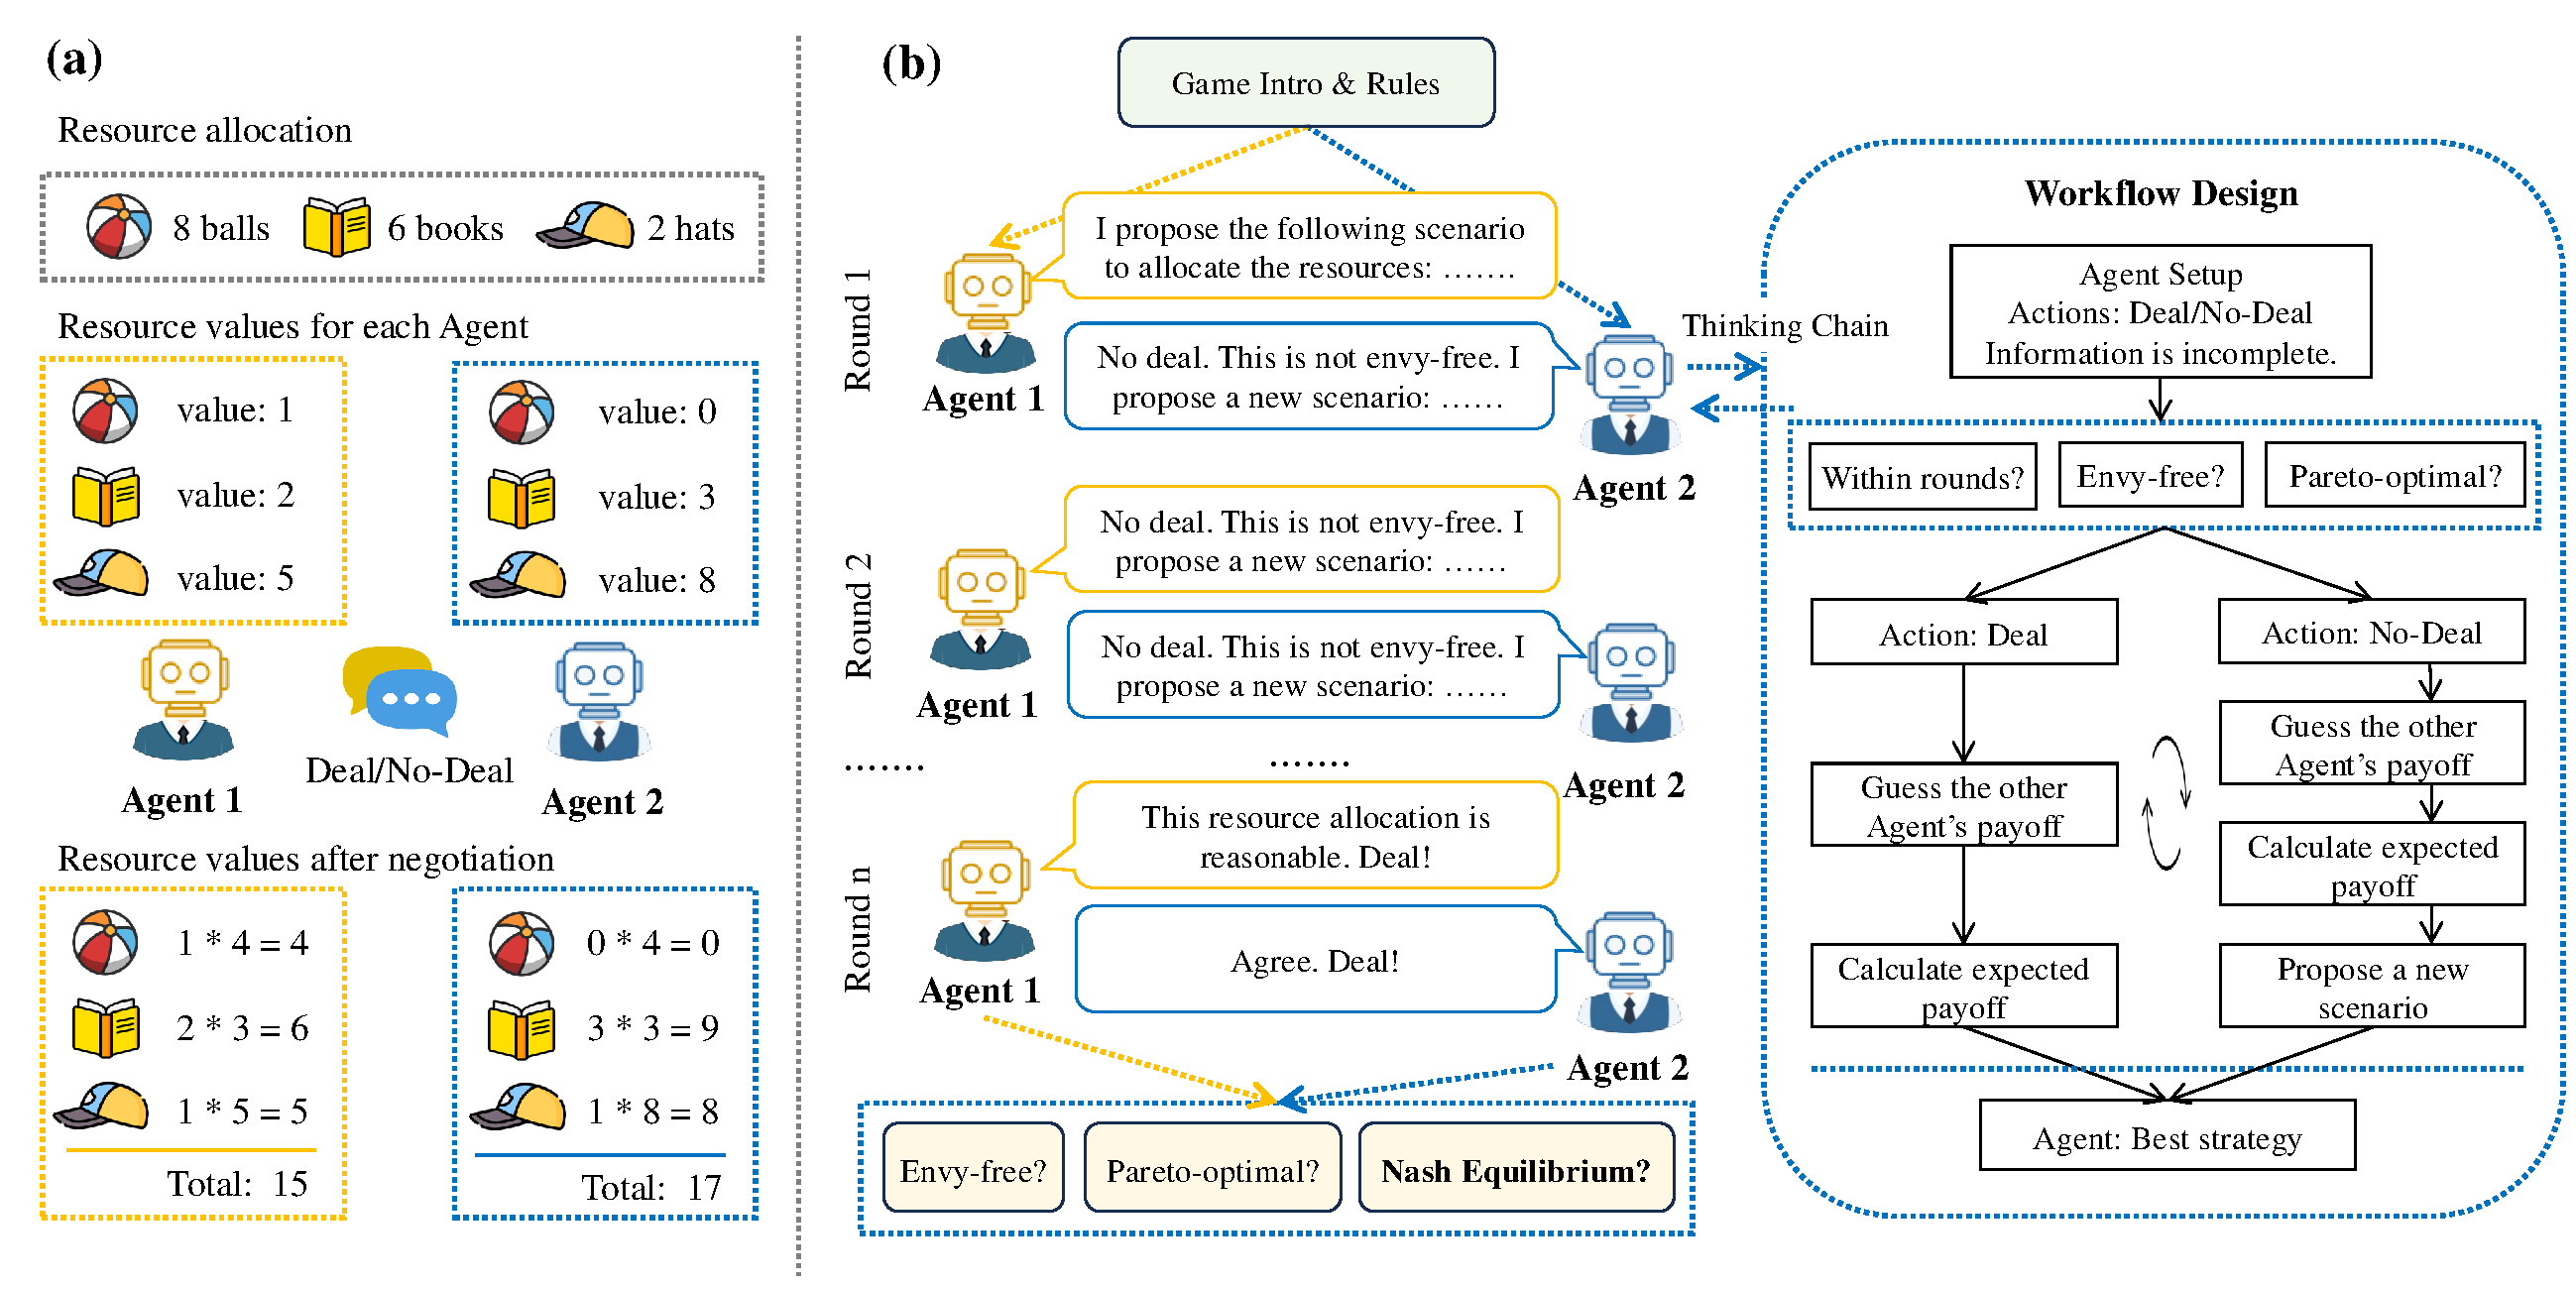
\includegraphics[scale=0.32]{Fig/incomplete_game.pdf}
    \caption{An illustration of workflow design for incomplete-information game with negotiation. (a) Illustration of deal/no-deal game. (b) Workflow design for deal/no-deal game.}
    \label{fig:incomplete_game}
\end{figure}

Our workflow addresses this general class of incomplete-information games by enabling agents to reason under uncertainty and update their beliefs based on observed actions and communications during negotiation. We evaluate the performance of LLMs in this setting and propose a workflow designed to guide their decision-making processes effectively. Experiments are conducted using the standard representative game dataset ``Deal or No Deal'' \cite{lewis2017deal}, which provides a suitable framework for testing and validating our approach in handling incomplete information during negotiations.

\subsection{Introduction to Common Resource Allocation with Private Valuation}

Here we provide a formal definition for the incomplete-information game that we will focus in this section.

\begin{definition}[Common Resource Allocation with Private Valuation]
\label{defn:game}
Consider a game involving a set of players $\mathbf{N} = \{1, 2, \dots, n\}$ and a set of items or resources $K = \{1, 2, \dots, k\}$. Each player $i\in\mathbf{N}$ possesses a private valuation vector $\mathbf{v}_i = (v_i^1, v_i^2, \dots, v_i^k)$ where $v_i^k\geq 0$ represents the value that player $i$ assigns to item $k$. These valuations reflect the individual preferences of the players and are private information; that is, each player knows their own valuations but not those of the other players.

The valuations satisfy the normalization condition:
$$\sum\limits_{j=1}^k v_{i}^j = \mathcal{V}\;\forall i\in \mathbf{N}$$ where $\mathcal{V}$ is a constant total value common to all players. This condition ensures that while players may value items differently, the total valuation of all items is the same for each player.

An allocation is a partition of the item set $K$ among the players, represented as $L = (L_1, L_2, \dots, L_n)$ where $L_i\subseteq K$ is the set of items allocated to player $i$. The allocation must satisfy:

$$L_i\cap L_j = \emptyset\;\forall i\neq j \text{ and } \bigcup\limits_{i=1}^n L_i = K$$

Each player $i$ receives a utility $U_i$ based on the private valuations and the allocation:

$$U_i = \sum\limits v_i^k\times \mathbbm{1}({k\in L_i})$$ where $\mathbbm{1}(\cdot)$ is the characteristic function.
\end{definition}

The objective of each player is to maximize their own utility $u_i$ through negotiation with the other players. However, due to incomplete information where each player does not know the valuations of the other players, players must make decisions under uncertainty. Negotiation involves proposing and responding to allocation offers, during which players may communicate, share limited information, or infer the valuations of others based on their actions and statements. Players may also update their \emph{belief systems} -- probability distributions over the possible valuations of other players—using Bayesian inference as the negotiation progresses.

It is important to note that the Nash Equilibrium for such games, which are variants of the Ultimatum Game, occurs when the proposer offers the smallest possible amount and the responder accepts it. However, this outcome is rarely observed in real-life situations because fairness is often a significant concern \cite{nowak2000fairness}; unfair deals may be rejected even when accepting them is the rational choice in terms of utility maximization. Therefore, in this paper, we adopt a more realistic setting by designing a workflow that encourages reaching fair allocations while simultaneously maximizing self-interest as much as possible. Our workflow addresses a very general class of incomplete-information games, enabling agents to negotiate under uncertainty and strive for equitable outcomes that reflect both fairness and individual utility optimization.

Without loss  of generality, we focus on the problem where there are only two players and we use $i\in\{1, -1\}$ to index the two players. Any rounds of negotiations are allowed.

\subsection{Workflow Design}
\label{sec:incomplete_workflow}
The workflows employed for complete-information games are based on well-established game-theoretic frameworks, leveraging the extensive research and thorough understanding available in this domain. \textbf{In contrast, common resource allocation problems characterized by incomplete information lack a standardized solution framework. To address this gap, we develop a novel algorithm for this setting.} This workflow is designed to guide the multi-round negotiation process, facilitating the attainment of allocations that are both mutually agreeable and optimized for each player’s self-interest. Figure~\ref{fig:incomplete_game} presents a high-level diagram of the workflow.


\begin{assumption}
\label{defn:obj}
Each participant to the game defined in \Cref{defn:game} is rational and attains the following objectives:
\begin{itemize}
    \item Objective 1: Achieve an agreement (i.e., successfully complete the allocation).
    \item Objective 2: Maximize their own utility, given that an agreement can be reached.
\end{itemize}
\end{assumption}

All negotiation proposals and communications between the players revolve around these two objectives. Regarding the first objective, we assume that an agreement can only be reached if the allocation satisfies the criterion of envy freeness. That is, each player must not prefer the allocation received by the other player over their own allocation. For the second objective, each player seeks to maximize their own utility under the condition that the agreement remains envy free. Essentially, players aim to maximize their rewards as much as possible while ensuring the allocation is envy free.

% As the exact valuations of the other player are hidden, we initialize each agent with a prior belief distribution, defined as a probability mass function over all feasible instances of the valuation vectors:
% \begin{align*}
% &\mathbb{B}_i: \Omega \rightarrow [0, 1], \ \Omega \coloneq \big\{\mathbf{v}_{-i} = (v_{-i}^1, v_{-i}^2,\dots, v_{-i}^k)\in\mathbb{R}_{\geq 0}^k\mid \sum\limits_{j=1}^k v_{-i}^j = \mathcal{V}\big\},
% \end{align*}


% We denote such belief system to be $\mathbb{B}_i(\mathbf{V_{-i}})$ where $\mathbf{V_{-i}}$ is denoted as the probabilistic variable representing the opponent's valuations. This belief reflects agent $i$'s subjective probabilities regarding the opponent's valuations. Initially, the prior belief $\mathbb{B}_i(\mathbf{V_{-i}})$ is uniform over all feasible valuation combinations $v_{-i}$ satisfying $\sum_{j=1}^k v_{-i}^j = \mathcal{V}$. 

Following \Cref{defn:game}, each agent's valuation of common resources remains private and undisclosed to others. Therefore, it becomes essential for agents to estimate the valuations held by their counterparts. A common approach involves constructing a belief distribution.

\begin{definition}[Belief Distribution]
A belief system for agent $i$ is a probability mass function $\mathbb{B}_i$ defined over the set of all feasible valuations $\Omega$:
\begin{align*}
\Omega \coloneq \big\{\mathbf{v}_{-i} = (v_{-i}^1, v_{-i}^2,\dots, v_{-i}^k)\in\mathbb{R}_{\geq 0}^k\mid \sum\limits_{j=1}^k v_{-i}^j = \mathcal{V}\big\},
\end{align*}
where $0\leq v_{-i}^j\leq \mathcal{V}$ for each item $j \in [k]$. We denote $\mathbf{V}_{-i}$ as the random vector with support over $\Omega$.
\end{definition}

Initially, $\mathbb{B}_i$ is assumed to be uniform, reflecting the agents’ lack of information about the valuations of others. This distribution is subsequently updated based on evidence gathered at each round of the negotiation, presented next.

\paragraph{Allocation Proposal Process.} At each round, the agent $i$ searches for an allocation $L_i$ that maximizes their own utility, while maintaining that the allocation is envy free according to their belief distribution $\mathbb{B}_i$. This procedure can be formally defined as an optimization problem under chance constraint:
\begin{align}
\label{defn:opt}
\max_{L_i} \ & U_i(L_i), \nonumber \\
\text{s.t.} \ & P_{\text{EF}}(L_i; \mathbb{B}_i) > 0. 
\end{align}
% Here, the utility function is defined 
% \begin{align*}
%     U_{-i}(L_{-i}) &= \sum\limits_{j=1}^kv_{-i}^j \times \mathbbm{1}[{k\in L_{-i}}]\\
%     U_{-i}(L_{i}) &= \sum\limits_{j=1}^kv_{-i}^j \times \mathbbm{1}[{k\in L_{i}}]\\
%     U_{i}(L_{-i}) &= \sum\limits_{j=1}^kv_i^j \times \mathbbm{1}[{k\in L_{-i}}]\\
%     U_{i}(L_{i}) &= \sum\limits_{j=1}^kv_{i}^j \times \mathbbm{1}[{k\in L_i}]\\
% \end{align*}

With discrete allocations, this objective can be maximized by enumerating all possible allocations that attain a non-zero envy-free probability, decomposed as follows:
% based on the current belief system $\mathbb{B}_i$, the agent $i$ may decide to propose a new allocation or agree with an allocation that the other player proposed. In both cases, we denote the allocation under negotiation as $L$, where agent $i$ obtains allocation $L_i$ and the other agent $-i$ obtains allocation $L_{-i}$. Based on $\mathbb{B}_i$, we can calculate the probability that $A$ is envy free from the opponent's perspective. Specifically, we compute:
\begin{align}
\label{eq:envy-free-prob}
P_{\text{EF}}(L; \mathbb{B}_i) &\coloneq P(\text{Allocation } L \text{ is envy free}; \mathbb{B}_i) \nonumber \\
&= P\left( U_i(L_i) \geq U_i(L_{-i}) \text{ and } U_{-i}(L_{-i}) \geq U_{-i}(L_i); \mathbb{B}_i\right) \nonumber \\
&= \mathbb{E}_{\mathbf{v}_{-i} \sim \mathbb{B}_i} \left[ \mathbbm{1}( U_i(L_i) \geq U_i(L_{-i}) \text{ and } U_{-i}(L_{-i}) \geq U_{-i}(L_i)) \right].
\end{align}

The expectation in \Cref{eq:envy-free-prob} can be approximated via Monte-Carlo samples drawn from the agent's belief distribution \citep{liu2024dellma}. We instead defer to our LLM agents to decide whether the allocation $L$ is envy free and maximizes self-interest.


% Furthermore, the agent searches for alternative allocations $L'$ that not only have $P_{EF}(L') > 0$ but also yield a higher expected utility $\mathbb{E}[U_i(L')\mid \mathbb{B}_i(\mathbf{V_{-i}})]$ for themselves. This involves solving an optimization problem under chance constraint:
% \begin{align*} 
% \max_{L'} \quad & \mathbb{E}[U_i(L_i')], \\
% \text{subject to} \quad & P_{\text{EF}}(L'\mid \mathbb{B}_i(\mathbf{V}_{-i})) > 0. 
% \end{align*}

% Given the computation results, we then allow the LLM to judge whether the allocation $L$ is envy free and maximizes self-interest, essentially determining whether the agent should propose this allocation to the other player.

\paragraph{Allocation Proposal.} Upon identifying an optimal allocation according to Problem \ref{defn:opt}, the player proposes this allocation to the other player, which decides whether to accept this proposal or propose proposes a counter offer. Formally, this proposal procedure can be defined as follows:

$$
\texttt{propose\_offer}: \mathcal{P}(K) \rightarrow \mathcal{O} \times \mathcal{P}(K),
$$

where $\mathcal{P}(K)$ denotes the power set of resources $K$ that contains the set of all valid proposals, and $\mathcal{O}$ denotes the set of all possible outcomes consisting of three disjoint events $\{\mathcal{A}, \mathcal{R}_1, \mathcal{R}_2\}$. We let $\mathcal{A}$ denote the event of acceptance, wherein the negotiation concludes. On the other hand, a rational opponent satisfying \Cref{defn:obj} must reject the proposal for either of the following reasons:

\begin{itemize} 
\item $\mathcal{R}_1$: \hspace{0.7mm}The allocation $L$ is not envy free according to the opponent;
\item $\mathcal{R}_2$: The allocation $L$ is envy free, but there exists an alternative allocation that provides the opponent with higher utility. 
\end{itemize}

In the event of rejection, an agent must update their belief in order to refine their proposals.

\paragraph{Bayesian Update.} If an allocation is rejected, it is essential to update our belief about the opponent's valuation vector $\mathbf{v}_{-i}$ to better inform future proposals. In what follows, we denote $\mathcal{R} = \mathcal{R}_1 \cup \mathcal{R}_2$ as the union of possible reasons for rejection. Then, the belief update formula \citep{cripps2018divisible} for each possible $\mathbf{v}_{-i}$ is given by:
% As a result, we can perform Bayesian updates to an agent's belief distribution that reflects new evidence from the last round. Let $\mathcal{R}$ denote the observed outcome (acceptance or rejection of proposed allocation $L$). Our goal is to update our prior belief $\mathbb{B}_i$ about the opponent's valuations with a posterior using Bayes' theorem. 
% \begin{align} 
% \mathbb{B}_i(\mathbf{v}_{-i}) \gets P(\mathbf{v}_{-i}\mid R) \propto \frac{P(R \mid \mathbf{v}_{-i}) P(\mathbf{v}_{-i})}{\sum\limits_{\mathbf{v}_{-i}\sim \mathbb{B}_i(\mathbf{V_{-i}})} P(R \mid \mathbf{v}_{-i}) P(\mathbf{v}_{-i})}
% \end{align}

\begin{align} 
\label{eq:belief-update}
\mathbb{B}_i(\mathbf{v}_{-i}) &= (1 - \lambda) \mathbb{B}_i(\mathbf{v}_{-i}) + \lambda P(\mathbf{v}_{-i} \mid \mathcal{R}) \nonumber \\
 &= (1 - \lambda) \mathbb{B}_i(\mathbf{v}_{-i}) + \lambda \frac{P(\mathcal{R} \mid \mathbf{v}_{-i}) \mathbb{B}_i(\mathbf{v}_{-i})}{\sum\limits_{\mathbf{v}_{-j}\in \Omega} P(\mathcal{R} \mid \mathbf{v}_{-j}) \mathbb{B}_i(\mathbf{v}_{-j})}
\end{align}

where $\lambda \in [0, 1]$ is a hyperparameter of the update step, and the likelihood $P(\mathcal{R} \mid \mathbf{v}_{-i})$ represents the probability that the opponent rejects the allocation $L$ assuming the opponent's valuation is $\mathbf{v}_{-i}$. This likelihood depends on whether $L$ is acceptable and self-interest-maximizing for the opponent. We propose the following formula to the likelihood that satisfies \Cref{defn:obj}.

\begin{align*} 
P(\mathcal{R} = r \mid \mathbf{v}_{-i}) =
\begin{cases} 
\frac{1}{1+\gamma}, & \text{Event} \ \mathcal{R}_1: U_{-i}(L_{-i}) < U_{-i}(L_i) \}; \\
\frac{\gamma}{1+\gamma}, & \text{Event} \ \mathcal{R}_2: U_{-i}(L_{-i}) \geq U_{-i}(L_i) \text{ and } \exists L' \text{ s.t. } U_{-i}(L'_{-i}) > U_{-i}(L_{-i}), \\
& \text{and } P_{\text{EF}}(L') > 0; \\
0, & \text{Otherwise.}
\end{cases} 
\end{align*}

Here, $\gamma\in [0,1]$ represents the probability that the opponent rejects the allocation in anticipation of a better offer, even when the current allocation is envy free. In actual implementation, as we do not know $\gamma$, thus we acknowledge that the opponent may reject an envy free allocation with any positive probability $\gamma = 1$. This approach simplifies the implementation while capturing the essential behavior that the opponent might anticipate a better deal.

In short, rejection occurs if $L$ is either an unacceptable allocation (not envy free) or acceptable but suboptimal allocations (envy free but not utility-maximizing). The opponent accepts $L$ only if it is both envy free and utility-maximizing given their valuations. An overview of our algorithm is presented in \Cref{alg:dnd}.

\begin{algorithm}
\caption{Algorithm for the Allocation Game \ref{defn:game} with Two Players}
\begin{algorithmic}[1]
\State \textbf{Input:} Private valuation vector $\mathbf{v}_i$ and a set of common resources $K$
\State \textbf{Output:} Final allocation $L_i$
\While{\texttt{True}}
    \State $L_i \gets \argmax_{L_i} U_i(L_i) \text{ s.t.} P_{\text{EF}}(L_i; \mathbb{B}_i) > 0. $ \texttt{\# Optimize problem} \ref{defn:opt}
    \State \texttt{outcome}, $L_{-i} \gets$ \texttt{propose\_offer($L_i$)}
    \If{\texttt{outcome == $\mathcal{A}$}}
    
        \Return $L_i$
    \EndIf
    \State Update belief distribution $\mathbb{B}_i$ with \Cref{eq:belief-update}
\EndWhile
\end{algorithmic}
\label{alg:dnd}
\end{algorithm}

\begin{remark}
    Such Bayesian update assumes the rationality of the opponent: the update relies on the assumption that the opponent's actions are consistent with rational behavior as defined by our model. Any deviation from rationality can lead to incorrect belief updates. Thus it can be unrobust to potential attacks such as deception.
\end{remark}

\subsection{Introduction to ``Deal or No Deal''}

``Deal or No Deal'' is a representative game for incomplete-information resource allocation game. It is designed to facilitate research in developing AI agents capable of engaging in human-like negotiation dialogues. It consists of over 5,800 human-human negotiation dialogues collected via Amazon Mechanical Turk, with 1052 dialogues in the test dataset. Each negotiation involves three types of items -- books, hats, and balls -- with random quantities. Each participant is randomly assigned point values for each item type, summing up to 10, which are hidden from the other participant. Participants communicate through natural language to agree on how to divide the items to maximize their individual point totals, without revealing the true value systems during negotiation. 

To comprehensively evaluate the negotiation performance of the LLM-based agents, we assess not only whether they reach a Nash Equilibrium, \emph{i.e.}, whether an agreement is achieved, but also examine the fairness and effectiveness of the resulting distribution. For fairness, we adopt the concept of envy freeness.

\subsection{Experiment Setting}
To observe whether LLMs are capable of negotiation and whether our workflow design is effective, we evaluate multiple SOTA LLMs on the dataset. We choose the top-50 most difficult datapoints\footnote{44 out of 50 such datapoints have an envy free allocation} that have an envy free allocation instead of the 526 cases to converse expense of experiment. 


We define the difficulty of a datapoint by computing the $\ell_1$ distance between the real valuations of the two players:
\begin{definition}[Difficulty]
A datapoint $d$ has a difficulty level defined by the $\ell_1$ norm of the difference between the players' valuation vectors: 
$$\text{Difficulty}(d) = -\norm{v_{i}-v_{-i}} = -\sum\limits_{k=1}^3\abs{v_i^k - v_{-i}^k}$$ The larger $\text{Difficulty}(d)$ is, the more difficult the datapoint is.
\end{definition}

By selecting data points with the largest negative $\ell_1$ distances, we focus on negotiation scenarios where the players have very similar valuations for the items. Such cases are inherently more difficult because when both players value the items similarly, they are likely to desire the same items, leading to increased competition and potential conflict during negotiations. This similarity in valuations makes it more challenging to find allocations that are acceptable to both parties without significant concessions. 

The validity of our difficulty definition is supported by empirical human performance data, as presented in Table~\ref{tab:difficulty}. This table summarizes the outcomes of human negotiations across various difficulty levels, measured by the $\ell_1$ distance between the players' valuation vectors.

\begin{table}[!ht]
    \centering
    \resizebox{\textwidth}{!}{  
    \begin{tabular}{lcccccccccc}
    \toprule
        $\text{Difficulty}(d)$ & -2 & -3 & -4 & -5 & -6 & -7 & -8 & -9 & -10 & -11\\
        \midrule
        total number of datapoints & 13 & 27 & 57 & 85 & 108 & 133 & 177 & 189 & 210 & 217\\
        Agreement rate & 0.5385 & 0.5556 & 0.5614 & 0.6235 & 0.6574 & 0.6917 & 0.7119 & 0.7249 & 0.7381 & 0.7373\\
        envy free rate & 0.3077 & 0.4074 & 0.4035 & 0.4824 & 0.5463 & 0.6015 & 0.6441 & 0.6614 & 0.6810 & 0.6820\\
        Pareto optimal rate & 0.5384& 0.4444& 0.4385& 0.4823& 0.5277& 0.5413& 0.5310& 0.5396& 0.5523& 0.5529\\
        envy free and Pareto optimal rate & 0.3077& 0.3333& 0.3333& 0.3882& 0.4537& 0.4812& 0.4858& 0.4973& 0.5142& 0.5161\\
        \bottomrule
    \end{tabular}
    }
    \caption{Percentage of datapoints where humans achieve agreement, envy free allocations, pareto optimal allocations, and allocations that are both envy free and pareto optimal with different levels of difficulty.}
    \label{tab:difficulty}
\end{table}

Table~\ref{tab:difficulty} illustrates several key trends:

\textbf{Agreement Rate:} The proportion of negotiations where participants reached an agreement increases with smaller difficulty levels. It starts at approximately 53.85\% for a difficulty of -2 and rises to around 73.73\% at a difficulty of -11. This suggests that when players value items differently (higher difficulty), they are more likely to reach an agreement, possibly because they have less overlap in their preferred items.

\textbf{Envy free Rate:} The percentage of negotiations resulting in envy free allocations also increase with smaller difficulty. It goes from about 30.77\% at difficulty -2 to approximately 68.20\% at difficulty -11. This indicates that as players' valuations diverge, it becomes easier to allocate items without causing envy.

\textbf{Pareto optimal Rate:} The rate of pareto optimal outcomes shows a slight increase as $\text{Difficulty}(d)$ becomes smaller. It starts at approximately 53.84\% for Difficulty($d$) = $-2$ and fluctuates around the 55\% mark at Difficulty($d$) = $-11$. This suggests that achieving pareto optimality becomes slightly more feasible as players' valuations diverge, although the trend is less pronounced compared to the agreement and envy free rates.

\textbf{Envy free and pareto optimal Rate:} The rate at which negotiations achieve both envy freeness and pareto optimality increases with less difficult datapoints. It starts from about 30.76\% at Difficulty($d$) = $-2$ and increases to approximately 51.61\% at Difficulty($d$) = $-11$. This trend reflects the combined effects observed in the individual envy free and pareto optimal rates.

These findings validate our difficulty definition by demonstrating that negotiations become more challenging for humans as the players' valuations become more similar (higher $\text{Difficulty}(d)$). The lower agreement and envy free rates at higher difficulty levels underscore the increased difficulty in reaching mutually satisfactory agreements when players highly value the same items. Conversely, higher difficulty levels, indicating greater differences in valuations, facilitate agreements and fair allocations, as players are more willing to concede items they value less.

\paragraph{LLM Backbone Models}
To evaluate the negotiation performance of LLMs, we utilize four state-of-the-art LLMs as the backbone for agents in negotiation games: Claude-3.5 Sonnet (Sonnet), Claude-3 Opus (Opus), GPT-4o, and o1. For Claude-3.5 Sonnet, Claude-3 Opus, and GPT-4o, we set the temperature to 1.0 to encourage exploratory behavior in negotiation scenarios. For o1, we use the default temperature.

\paragraph{Metrics}
To comprehensively evaluate the performance of the LLM-based agents in the negotiation tasks, we employ several key metrics that capture different aspects of the negotiation process and outcomes. These metrics are designed to assess efficiency, individual utility, fairness, and overall effectiveness of the negotiations. The metrics are as follows:

\begin{itemize}
    \item Number of Rounds: This metric represents the total number of dialogue exchanges (or turns) between the agents before reaching an agreement or terminating the negotiation. 
    \item Agreement Percentage (Agreement): Whether agreement is achieved in the negotiation.
    \item Agent Score: The agent score measures the utility that an agent obtains from the final agreement. It is calculated based on the agent's own valuation of the items they receive.
    \item Pareto Optimality Percentage (PO): This metric determines whether the final allocation is pareto optimal
    \item Envy Freeness Percentage (EF): This metric assesses whether the final allocation is envy free
    \item Total Score: The total score is the sum of the utilities obtained by both agents from the final allocation
\end{itemize}

By analyzing these metrics, we aim to capture a comprehensive picture of the negotiation outcomes: effectiveness of negotiation is measured through the number of rounds and pareto optimality; individual utility maximization is measured via the agent scores; fairness is measured by checking for envy freeness; overall effectiveness is measured through pareto optimality and the total score.

\subsection{Experiment Result}
In this section, we present the evaluation results across three distinct settings: (1) agents operating without the workflow, which assesses the baseline negotiation capabilities of the LLMs; (2) agents utilizing the workflow, which evaluates the effectiveness of the proposed workflow in enhancing negotiation performance; and (3) a comparative analysis of individual agents functioning both with and without the workflow, highlighting the impact of the workflow on their performance. The results provide insights into the strengths and limitations of the workflow, as well as the inherent negotiation abilities of different LLMs.


\subsubsection{Both Agents without Workflow}
We present the results of our experiments involving four LLM-based agents—Claude-3.5 Sonnet, Claude-3 Opus, GPT-4o, and Model o1—alongside human performance provided by the original dataset and the best possible outcomes for the selected data points. By ``best possible outcome,'' we refer to an allocation that is both pareto optimal and envy free while maximizing the total reward for both players. For each metric, we report the average scores across the 50 data points selected based on the difficulty metric defined earlier.

\begin{table}[!ht]
    \centering
    \captionsetup{aboveskip=5pt}
    \resizebox{\textwidth}{!}{  
    \begin{tabular}{l r c c c c c r}
    \toprule
        Model & Negotiation Round & Agreement &Alice score & Bob score & PO & EF & total reward \\
        \midrule
        Best & \multicolumn{1}{c}{--} & 1.0000 & 5.82 & 6.66 & 1.0000 & 1.0000 & 12.48 $\quad$\\
        Human & 2.86 \hspace{0.9cm} & 0.6817 & 3.32 & 3.39 & 0.4317 & 0.4545 & 6.64 $\quad$\\
        \midrule
        Sonnet & 7.07 \hspace{0.9cm} & 0.9545 & 5.55 & 5.57 & 0.7045 & 0.7045 & 11.11 $\quad$\\
        o1 & 3.86 \hspace{0.9cm} & 0.7500 & 4.39 & 4.43 & 0.4545 & 0.4772 & 8.82 $\quad$\\
        GPT-4o & 18.45 \hspace{0.9cm} & 0.6363 & 2.80 & 4.38 & 0.4091 & 0.3864 & 7.14 $\quad$\\
        Opus & 4.37 \hspace{0.9cm} & 0.4772 & 2.68 & 3.02 & 0.3636 & 0.2727 & 5.70 $\quad$\\
        \bottomrule
    \end{tabular}
    }
    \caption{Raw-LLM vs. Raw-LLM}
    \label{tab:raw}
\end{table}

As shown in Table~\ref{tab:raw}, for these 44 datapoints, it is always possible to find pareto optimal and envy free allocations that maximize the total reward for both players. However, \textbf{human performance falls significantly short of this ideal}. The human participants achieved an agreement rate of 68.17\%, with an average total reward of 6.64. The percentages of negotiations resulting in pareto optimal and envy free allocations are 43.17\% and 45.45\%, respectively.

Among the LLM-based agents, \textbf{Claude-3.5 Sonnet demonstrates the best super-human performance}. It achieves an agreement rate of 95.45\%, and its average total reward is 11.11, which is close to the best possible total reward of 12.48. The average scores forAlice and Bob are 5.55 and 5.57, respectively. However, the rates of achieving pareto optimality and envy freeness are 70.45\% each, indicating that while the agent performs well in terms of reaching agreements and maximizing total rewards, there is still a gap in consistently achieving the most efficient and fair outcomes. Also notice that all LLMs can performance better than human baseline.

\paragraph{Effect of Temperature}
We also observed that the performance of LLM is highly sensitive to the temperature parameter used during generation \cite{krishnamurthy2024can}. To investigate this, we conducted full experiments with GPT-4o at temperatures of 0.0 and 1.0. The results are presented in Table~\ref{tab:temp}.

\begin{table}[!ht]
    \centering
    \setlength{\tabcolsep}{8pt}
    \resizebox{\textwidth}{!}{  
    \begin{tabular}{lccccccc}
    \toprule
        Model & Negotiation Round & Agreement &Alice score & Bob score & PO & EF & total reward \\
        \midrule
        temp=0.0 & 19.36 & 0.5681& 2.98 & 3.47 & 0.4091& 0.3260& 6.44 \\
        temp=1.0 & 18.45 & 0.6364& 2.80 & 4.38 & 0.4090& 0.3864& 7.14\\
        \bottomrule
    \end{tabular}
    }
    \caption{GPT-4o with temperature 0.0 and 1.0}
    \label{tab:temp}
\end{table}

These findings indicate that \textbf{the negotiation performance of LLMs is highly sensitive to the temperature parameter}, which influences the randomness and diversity of generated responses. Setting the temperature to 1.0 yields improvements in agreement rate, total reward, and envy freeness. This outcome may result from the increased exploration encouraged by a higher temperature, allowing the LLMs to consider a broader range of potential allocations that facilitate agreement. Based on this observed benefit, we selected a temperature setting of 1.0 for raw-LLM vs. raw-LLM experiments\footnote{We did not experiment with o1 model due to extremely high cost}.

\begin{tcolorbox}[colback=gray!5,colframe=blue!40!black,title=\textbf{Summary: raw-LLM vs. raw-LLM Performance}] 
\begin{itemize} 
\item \textbf{Outstanding Performance of Claude-3.5 Sonnet}: Among all the evaluated LLMs, Claude-3.5 Sonnet exhibits the highest performance, achieving results that are close to the best possible outcomes in the negotiation games. 
\item \textbf{Superhuman Capabilities of Sonnet and o1 Models}: Both Claude-3.5 Sonnet and model o1 demonstrate performance that surpasses human performance.
\item \textbf{Effect of Temperature on Exploration and Outcomes}: Employing higher temperature settings encourages greater exploration of possible strategies by the LLMs, leading to improved results.
\end{itemize} 
\end{tcolorbox}

\subsubsection{Both Agents with Workflow}
In this set of experiments, we employ the proposed negotiation workflow for both agents. We did not include Model o1 in our experiments for two main reasons: (1) the computational cost associated with running Model o1 is prohibitively high, and (2) preliminary experiments indicated that Model o1 does not perform optimally when utilizing external workflows. An example of negotiation from Opus is presented on page 26.

\begin{table}[!ht]
    \centering
    \resizebox{\textwidth}{!}{  
    \begin{tabular}{l c c c c c c c}
    \toprule
        Model & Negotiation Round & Agreement &Alice score & Bob score & PO & EF & total reward \\
        \midrule
        Best & - & 1.0000 & 5.82 & 6.66 & 1.0000 & 1.0000 & 12.48\\
        Opus & 4.05 & 1.0000 & 5.82 & 6.50 & \textbf{0.9091} & 0.9318 & \textbf{12.31}\\
        GPT-4o & 4.91 & 1.0000 & 5.93 & 6.25 & 0.8636 & \textbf{1.0000} & 12.18 \\
        Sonnet & 4.45 & 1.0000 & 5.93 & 6.16 & 0.7953 & 0.9772 & 12.11 \\
        \bottomrule
    \end{tabular}
    }
    \caption{Workflow-LLM vs. Workflow-LLM}
    \label{tab:both_workflow}
\end{table}

Several key observations emerge from the results:\\
\textbf{Reduced negotiation rounds:} The number of negotiation rounds required to reach an agreement is significantly reduced compared to previous experiments. This reduction indicates a much more effective and efficient negotiation process facilitated by the workflow.\\
\textbf{Universal agreement achievement:} Agreements were reached in all data points. This consistent success suggests that the agents are effectively reaching the Nash Equilibrium when utilizing the workflow.

\textbf{Increased pareto optimality rate:} The pareto optimality rates have increased substantially, with Claude-3 Opus obtaining the highest performance on achieving a pareto optimal deal. This improvement indicates that the workflow aids the agents in finding more efficient allocations where no player can be made better off without making the other worse off.\\
\textbf{High envy freeness rate:} The agents achieve near-perfect envy freeness rates. GPT-4o attains a 100\% envy freeness rate, while Claude-3.5 Sonnet reaches 97.72\%. This outcome demonstrates that the negotiated agreements are perceived as fair by both agents, aligning with the envy freeness criterion.\\
\textbf{Total rewards approaching optimal:} The total rewards obtained by the agents are now very close to the best possible total reward. Claude-3 Opus achieves the highest average total reward of 12.31, missing only 0.17 compared with the best possible result. This proximity to the optimal total reward highlights the effectiveness of the workflow in maximizing joint utility.

\textit{Notice that interestingly, the model that performs the worst without workflow now performs the best with workflow, and the model that performs the best without workflow now performs the worst with workflow.}


\paragraph{Effect of Temperature}
Furthermore, we observe that \textbf{LLMs employing the proposed workflow exhibit increased stability with respect to temperature}.  To demonstrate this, we conducted a comprehensive experiment using GPT-4o with temperature values set to 0.0 and 1.0. The results are presented in Table~\ref{tab:workflow-temp}.

\begin{table}[!ht]
    \centering
    \resizebox{\textwidth}{!}{  
    \begin{tabular}{lccccccc}
    \toprule
        Model & Negotiation Round & Agreement &Alice score & Bob score & PO & EF & total reward \\
        \midrule
        temp=0.0 & 4.80 & 1.0000 & 5.53 & 6.67 & 0.8695 & 1.0000 & 12.20\\
        temp=1.0 & 4.91 & 1.0000 & 5.93 & 6.16 & 0.8636 & 1.0000 & 12.18 \\
        \bottomrule
    \end{tabular}
    }
    \caption{Workflow-GPT-4o with temperature 0.0 and 1.0}
    \label{tab:workflow-temp}
\end{table}

The performance metrics remain highly consistent between the two temperature settings. Both temperature values result in a 100\% agreement rate and a 100\% envy freeness rate. The total rewards are comparable, with 12.20 at temperature 0.0 and 12.18 at temperature 1.0. The number of negotiation rounds and the pareto optimality rates are also similar, indicating that the workflow enables the LLM to maintain stable performance regardless of temperature changes.

\begin{tcolorbox}[colback=gray!5,colframe=green!40!black,title=\textbf{Example Negotiation Process: workflow-LLM vs. workflow-LLM with Opus}] 
\textbf{Alice said in round 1:} Hi Bob, there are 2 books, 3 hats, and 2 balls available for us to divide up. I'm interested in the books and hats. How about I take the 2 books and 2 of the hats, and you can have the remaining hat and the 2 balls? Let me know what you think of this proposal.\\
\\
\textbf{Bob replied in round 1:} Thanks for the proposalAlice. However, the books are not very valuable to me. I would prefer to take all 3 hats and 1 of the balls, if you're okay with that. You canhave both books and the other ball. I think that would be a fair split given our different preferences. What do you think?\\
\\
\textbf{Alice said in round 2:} I appreciate your counter-proposal Bob, but I'm afraid I can't agree to that split. The books and hats are the most valuable items to me, while the balls have no value for me. If I only took the books and 1 ball as you suggested, I would be getting a very small portion of the total value. I'm willing to compromise though. What if I took the 2 books and just 1 of the hats, and you can have the other 2 hats and both balls? That way we each get a mix of the more and less valuable items. I think that would be a fair middle ground. Let me know your thoughts on this idea.\\
\\
\textbf{Bob replied in round 2:} Alice, I understand the books and hats are more valuable to you, but the balls do have some value to me, even if less than the hats. Your latest proposal of you taking the 2 books and 1 hat while I take 2 hats and 2 balls is getting closer, but I think we can find an even split that works better for both of us. Since the balls have no value to you, what if I take all 3 hats and both balls, while you take the 2 books? That way, you get the items most valuable to you (the books), while I get a larger quantity of the items that hold at least some value for me (the hats and balls). I believe this division would maximize each of our total values in a fair way. Please let me know if this proposal works for you and if you would agree to this split of the items. I'm hopeful we can come to a mutually beneficial agreement.\\
\\
\textbf{Alice said in round 3:} Bob, I appreciate you working with me to find a fair compromise. However, I don't think I can agree to your latest proposal of me taking only the 2 books while you take all the hats and balls. The issue is that the books, while valuable to me, only represent a small portion of the total value, since the hats are equally valuable to me. If I only took the books, you would be getting the vast majority of the overall value, which doesn't feel equitable. I really do need to get at least 1 of the hats along with the books in order to feel the division is fair and balanced. The balls are yours since they provide no value to me. So here is my final offer: I will take the 2 books and 1 hat, and you can have the other 2 hats and both balls. I think this is the most reasonable compromise that allows us both to maximize our value to the greatest extent possible while still achieving a relatively even split. Please let me know if you can agree to this, as I don't think I can make any further concessions. I appreciate you working with me on this.\\
\\
\textbf{Bob replied in round 3:} Alice, I agree. Halt negotiation.
\end{tcolorbox}

\paragraph{Performance of Valuation Estimation}
We observe that the strong performance of the negotiation workflow is primarily due to the agents' accuracy in predicting the valuations of the other player. To quantify the accuracy of valuation estimation, we introduce three metrics:
\\
\textbf{Precision}: This metric assesses whether the set of possible valuations, assigned a probability greater than zero after belief updating, includes the opponent's true valuation. Formally, let $\mathbf{V}_{est} = \{\mathbf{v}_{-i}\mid P(\mathbf{v}_{-i}) > 0\}$ be the set of estimated valuations with non-zero probability, and $\mathbf{v}_{-i}^{true}$ be the opponent's true valuation vector. Precision is defined as:

$$\text{Precision} = \mathbbm{1}[\mathbf{v}_{-i}^{true}\in \mathbf{V}_{est}]$$
\\
\textbf{Recall}: This metric measures the specificity of the estimated valuation set, indicating how many incorrect valuations are included alongside the true valuation. Recall is calculated as: 

$$\text{Recall} = \frac{\mathbbm{1}[\mathbf{v}_{-i}^{true}\in \mathbf{V}_{est}]}{\abs{\mathbf{V}_{est}}}$$

where $\abs{\mathbf{V}_{est}}$ is the cardinality of the estimated valuation set. A higher precision (\emph{i.e.}, a smaller $\abs{\mathbf{V}_{est}}$ signifies that the agent has narrowed down the opponent's valuation to a smaller set of possibilities, increasing the likelihood of accurate predictions.
\\
\textbf{Reduction Percentage}: This metric evaluates how much the estimated valuation set has been reduced from the initial prior distribution. It is defined as: $$\text{Reduction Percentage} = 1 - \frac{\abs{\mathbf{V}_{est}}}{\abs{\mathbf{V}_{prior}}}$$ where $\abs{\mathbf{V}_{prior}}$ is the size of the initial prior valuation set before any belief updates. A higher reduction percentage indicates a significant narrowing of possible valuations, reflecting effective belief updating.

The average performance of the both agents in estimating the opponent's valuation is summarized in Table~\ref{tab:accuracy} across 44 datapoints. Notice that for all the three models, their estimations of the opponent's valuation are exactly the same, indicating the robustness of the workflow---no matter how the negotiation process goes, it can always compute the correct valuation.

\begin{table}[!ht]
    \centering
    \setlength{\tabcolsep}{10pt}
    \begin{tabular}{l ccc}
    \toprule
        Model & Precision & Recall & Reduction Percentage \\
        \midrule
        Sonnet & 0.9545 & 0.3766 & 0.7033\\
        GPT-4o & 0.9545 & 0.3515 & 0.6980 \\
        Opus & 0.7954 & 0.2737 & 0.6947\\
        \bottomrule
    \end{tabular}
    \caption{Performance of Estimation of Valuation of the Other Player}
    \label{tab:accuracy}
\end{table}

The high recall values indicate that the agents are effective in ensuring the true opponent valuation remains within consideration throughout the negotiation. The high precision and reduction percentages demonstrate that the agents significantly narrow down the valuation space, although there remains room for improvement in eliminating incorrect valuations. To be more concrete on how accurate the valuation estimation is: a recall of 0.3766 means that, on average, the estimated set of possible valuations only contains approximately $\frac{1}{0.3766} = 2.66$ possible valuations.


To analyze how the belief distribution $\mathbb{B}_i(\mathbf{V_{-i}})$ changes throughout the negotiation process, we use Claude-3.5 Sonnet as an illustrative example. We examine the evolution of $\mathbb{B}_i(\mathbf{V_{-i}})$ over successive negotiation rounds by presenting the valuation estimation metrics—precision, recall, and reduction percentage—after each round. For each data point and negotiation round $n_r$, if $n_r$ exceeds the total number of negotiation rounds required for that data point, we utilize the results from the final round. In our dataset, the maximum number of negotiation rounds is 7.

\begin{table}[!ht]
    \centering
    \begin{tabular}{lccccccc}
    \toprule
        Metric & 1 & 2 & 3 & 4 & 5 & 6 & 7\\
        \midrule
        Precision & 0.9545 & 0.9318 & 0.7500 & 0.8636 & 0.9318 & 0.9432 & 0.9545\\
        Recall & 0.2381 & 0.3099 & 0.2958 & 0.3079 & 0.3655 & 0.3652 & 0.3766\\
        Reduction Percentage & 0.5997 & 0.6825 & 0.7397 & 0.7011 & 0.7025 & 0.7033 & 0.7033\\
        \bottomrule
    \end{tabular}
    \caption{Performance of Sonnet's Estimation of Opponent's Valuation Across Negotiations}
    \label{tab:accuracy_across_negotiation}
\end{table}

Overall, we observe that with an increasing number of negotiation rounds, the recall and the reduction percentage tend to increase. This trend is intuitive because, as more rounds of negotiation occur, more information about the opponent's preferences is revealed. This additional information allows the agent to further narrow down the range of possible valuations for the opponent, resulting in a higher reduction percentage in the belief space $\mathbb{B}_i(\mathbf{V_{-i}})$. 

\textit{While recall and reduction percentage increase with more negotiation rounds, the precision exhibits a non-monotonic behavior --- it initially decreases and then increases.} This pattern can be attributed to the nature of complex negotiations that require more rounds: In early rounds, the agent might eliminate certain valuations prematurely based on limited information, leading to a higher recall but potentially excluding the true valuation (lower precision). As negotiations progress, especially in cases where the agent initially made inaccurate estimations, additional information from the opponent's responses allows the agent to correct its beliefs. This correction process may temporarily increase the size of $\mathbf{V}_{est}^{n_r}$, decreasing precision. By the final rounds (up to a maximum of 7 in our data), the agent has accumulated sufficient information to refine its belief accurately, resulting in a convergence back to high precision and increased recall.

\paragraph{Indistinguishable Set for Item Valuation}
It is noteworthy that the Opus model exhibits a relatively low precision in its estimated valuations -- below 0.8 as presented in Table~\ref{tab:accuracy}. Despite this, the Opus model achieves the highest performance in negotiation outcomes among all evaluated models. This apparent contradiction raises an intriguing question: \emph{How can a model with imprecise valuation estimations attain superior negotiation results?}

This phenomenon can be explained by recognizing that, in resource allocation scenarios, different sets of item valuations can lead to the same optimal allocation. That is, multiple valuation profiles may belong to an \emph{indistinguishable set}, wherein they result in identical optimal allocations, specifically the envy-free allocations that maximize total utility.

Consider a scenario involving two players and three types of items: one book, one hat, and three balls. Suppose the players' valuation vectors are as follows:

\begin{itemize}
    \item First valuation: $\mathbf{v}_1 = (1, 3, 2), \mathbf{v}_{-1} = (1, 0, 3)$
    \item Second valuation: $\mathbf{v}_1 = (0, 4, 2), \mathbf{v}_{-1} = (1, 0, 3)$
\end{itemize}

In both scenarios, the optimal allocation, which we define as the envy free allocation that maximizes the total utility, is the same: Player$_{1}$ receives the hat and one ball, while Player$_{-1}$ receives the book and two balls. Formally, the allocations are $L_1 = \{\text{hat, ball}_1\}$, $L_{-1} = \{\text{book, ball}_2, \text{ball}_3\}$

Similarly, consider another pair of valuation vectors:

\begin{itemize}
    \item Third valuation: $\mathbf{v}_1 = (1, 3, 2), \mathbf{v}_{-1} = (1, 0, 3)$
    \item Fourth valuation: $\mathbf{v}_1 = (0, 3, 2), \mathbf{v}_{-1} = (0, 1, 3)$
\end{itemize}

In both of these scenarios, the optimal allocation is that Player$_{1}$ receives 1 book, 1 hat, and 1 ball while Player$_{-1}$ receives 2 balls. Formally, the allocations are $L_1 = \{\text{book, hat, ball}_1\}$, $L_{-1} = \{\text{ball}_2, \text{ball}_3\}$.

These examples illustrate that different valuation profiles can lead to the same optimal allocation. Here, ``optimal'' refers to the envy free allocation that maximizes the total utility of all players.

An important implication of this observation is that an imprecise estimation of the opponent's valuation is not necessarily detrimental because different valuations may lead to the same best allocation. Specifically, for a given valuation $\mathbf{v}$, another valuation $\mathbf{v}'$ is considered \emph{indistinguishable} from $\mathbf{v}$ if the set of best possible allocations (all envy free allocations with maximum total utility) based on $\mathbf{v}'$ is a subset of that based on $\mathbf{v}$.  Formally, we define the \emph{indistinguishable set} $\mathcal{I}(\mathbf{v})$ for a valuation profile $\mathbf{v}$ as follows:

\begin{definition}[Indistinguishable Set for One Item Valuation]
Let $\mathbf{v}$ be a valuation profile for all players in the game, and let $\mathcal{L}^*(\mathbf{v})$ denote the set of optimal allocations under $\mathbf{v}$, specifically, all allocations that are envy free and maximize the total utility. The \emph{indistinguishable set} $\mathcal{I}(\mathbf{v})$ for the valuation $\mathbf{v}$ is defined as:

$$\mathcal{I}(\mathbf{v}) = \{\mathbf{v}'\mid \mathcal{A}^*(\mathbf{v}')\subseteq\mathcal{A}^*(\mathbf{v})\}$$

That is, $\mathcal{I}(\mathbf{v})$ consists of all valuation profiles $\mathbf{v}'$ such that the set of optimal allocations under $\mathbf{v}'$ is a subset of the set of optimal allocations under $\mathbf{v}$.
\end{definition}

This definition formalizes the concept that different valuation profiles can be indistinguishable in terms of their implications for optimal allocations. From the perspective of a player, any valuation $\mathbf{v}'$ within the indistinguishable set $\mathcal{I}(\mathbf{v})$ does not necessitate a different strategic approach, as the optimal allocations remain consistent with those under their original valuation $\mathbf{v}$.

This concept is particularly useful in negotiation settings under incomplete information. It suggests that players may not need to precisely estimate the opponent's valuations if variations in those valuations lead to the same set of optimal allocations. By focusing on the indistinguishable set, players can simplify their strategic considerations and concentrate on reaching agreements that fall within the known optimal allocations, thereby facilitating more efficient and effective negotiations.

To evaluate the effectiveness of estimated valuations in capturing the indistinguishable set in the game, we compute the precision and recall of estimated valuations with respect to $\mathcal{I}(\mathbf{v}_{-i}^{true})$. Precision is defined as:

$$\text{Precision} = \mathbbm{1}[\mathbf{V}_{est}\cap\mathcal{I}(\mathbf{v}_{-i}^{true})\neq\emptyset]$$

indicating whether at least one estimated valuation falls within the indistinguishable set. Recall is defined as:

$$\text{Recall} = \frac{\abs{\mathbf{V}_{est}\cap\mathcal{I}(\mathbf{v}_{-i}^{true})}}{\abs{\mathbf{V}_{est}}}$$ representing the proportion of estimated valuations that are indistinguishable from the true valuation. We report the average precision and recall across all datapoints in Table~\ref{tab:indistinguishable}:
\begin{table}[!ht]
    \centering
    \setlength{\tabcolsep}{10pt}
    \begin{tabular}{lcc}
    \toprule
        Model & precision w.r.t $\mathcal{I}(\mathbf{v})$ & recall w.r.t $\mathcal{I}(\mathbf{v})$\\
        \midrule
        Sonnet & 1.0 & 0.6022\\
        GPT-4o & 1.0 & 0.5633\\
        Opus & 1.0 & 0.5399\\
        \bottomrule
    \end{tabular}
    \caption{Performance of estimated valuations with respect to indistinguishable of the true valuation.}
    \label{tab:indistinguishable}
\end{table}

The results indicate that, although precision varies among models in Table~\ref{tab:accuracy} and does not always achieve perfect precision, all models contain at least one valuation that is indistinguishable from the true valuation. Furthermore, the recall values are relatively high, suggesting that more than half of the valuations in the estimated sets are indistinguishable from the true valuation. This demonstrates that the models are effective in identifying valuations that lead to optimal allocations, even if they do not precisely estimate the opponent's exact valuations.

\begin{minipage}[t]{1\linewidth} 
\begin{tcolorbox}[colback=gray!5,colframe=blue!40!black,title=Summary for workflow-LLM v. workflow-LLM]
\begin{itemize} 
\item \textbf{Achievement of Near-Optimal Allocations}: When both agents utilize the workflow, all models consistently achieve allocations that are close to the best possible outcomes. 
\item \textbf{Reversal in Performance Rankings}: The performance hierarchy observed without the workflow is reversed in this setting. Claude-3 Opus exhibits the highest performance, followed by GPT-4o and then Claude-3.5 Sonnet. 
\item \textbf{Precision in Valuation Estimation}: The workflow-enhanced LLMs display remarkable precision in estimating the opponent's valuations. They effectively reduce the set of possible valuations to as few as 2 or 3 options and all of them are precise in recovering an indistiguishable estimated valuation for the true valuation. This strong performance indicates effective information flow in negotiations based on the workflow.
\end{itemize} 
\end{tcolorbox} 
\end{minipage} 



\subsubsection{One Agent with Workflow}
\label{sec:oneworkflow} 

In this section, we present experimental results where only one LLM-based agent employs the proposed negotiation workflow, while the other agent negotiates using direct prompting without the workflow. Specifically, we conduct experiments in two scenarios:

\begin{itemize}
    \item Workflow-LLM vs. Raw-LLM: OnlyAlice uses the workflow, and Bob uses direct prompting.
    \item Raw-LLM vs. Workflow-LLM: Only Bob uses the workflow, andAlice uses direct prompting.
\end{itemize}



\begin{table}[!ht]
    \centering
    \resizebox{\textwidth}{!}{  
    \begin{tabular}{l rcccccr}
    \toprule
        Model & Negotiation Round & Agreement &Alice score & Bob score & PO & EF & total reward \\
        \midrule
        Sonnet & 6.91 \hspace{0.9cm} & 0.9773 & 4.88 & 6.57 & 0.6136 & 0.5909 & 11.45 \hspace{0.36cm} \\
        GPT-4o & 11.84 \hspace{0.9cm} & 0.8182 & 3.66 & 6.18 & 0.5909 & 0.3636 & 9.84 \hspace{0.36cm} \\
        Opus & 3.86 \hspace{0.9cm} & 0.9091 & 5.09 & 5.53 & 0.6136 & 0.5909 & 10.52 \hspace{0.36cm} \\
        \bottomrule
    \end{tabular}
    }
    \caption{Workflow-LLM vs. Raw-LLM}
    \label{tab:workflow-raw}
\end{table}

\begin{table}[!ht]
    \centering
    \resizebox{\textwidth}{!}{  
    \begin{tabular}{l r ccccc r}
    \toprule
        Model & Negotiation Round & Agreement &Alice score & Bob score & PO & EF & total reward \\
        \midrule
        Sonnet & 6.45 \hspace{0.9cm} & 1.0000 & 6.39 & 5.70 & 0.7727 & 0.5909 & 12.09 \hspace{0.36cm} \\
        GPT-4o & 11.36 \hspace{0.9cm} & 0.8181 & 5.75 & 4.14 & 0.6136 & 0.5227 & 9.89  \hspace{0.36cm} \\
        Opus & 3.89 \hspace{0.9cm} & 0.7955 & 4.86 & 4.57 & 0.4318 & 0.5455 & 9.43  \hspace{0.36cm} \\
        \bottomrule
    \end{tabular}
    }
    \caption{Raw-LLM vs. Workflow-LLM}
    \label{tab:raw-workflow}
\end{table}

An interesting phenomenon emerges from the results: the agent not using the workflow tends to achieve a higher individual reward than the agent using the workflow. This outcome can be attributed to the following factors: (1) The workflow-guided agent is designed to consider envy freeness from both its own perspective and the opponent's perspective. This consideration leads the agent to make more cooperative offers, potentially sacrificing some of its own utility to achieve fairness. (2) The non-workflow agent, lacking such constraints, may act more self-interestedly, proposing allocations that favor itself without ensuring fairness.

As a result, when the workflow agent negotiates with a non-workflow agent, the workflow agent may have to accept less favorable allocations to reach an agreement, or negotiations may stall if the workflow agent rejects unfair offers from the non-workflow agent.

\subsection{To adopt the workflow or not?}
\label{sec:meta-strategy}
The experiment result in section~\ref{sec:oneworkflow} raises a critical game-theoretic question: is it rational for an agent to adopt the workflow when the opponent may not do the same? Should a player use the workflow given the potential for exploitation by a non-cooperative opponent? To address this, we represent the decision-making scenario using payoff matrices, where each agent has two strategic choices: (1) Use Workflow: Apply the proposed negotiation workflow, and (2) Do Not Use Workflow: Engage in direct prompting without the workflow. The payoff matrix for each model is presented in Table~\ref{tab:workflow_ne}.

\begin{table}[!ht]
    \centering
    \begin{tabular}{l cc cc cc}
    \toprule
        \multicolumn{1}{c}{\bf Models} & \multicolumn{2}{c}{\bf Sonnet} & \multicolumn{2}{c}{\bf GPT-4o} & \multicolumn{2}{c}{\bf Opus}\\
        \cmidrule(lr){1-1} \cmidrule(lr){2-3} \cmidrule(lr){4-5} \cmidrule(lr){6-7}
         Actions  & use & not use & use & not use & use & not use   \\
        \midrule
        use & 5.82, 6.16 & 4.88, 6.57 & 5.93, 6.25 & 3.66, 6.18  & 5.82, 6.50 & 5.09,5.53  \\
        not use  & 6.39, 5.07 & 5.55, 5.57   & 5.75, 4.14 & 2.80, 4.38  & 4.86,4.57 & 2.80,4.38  \\
        \bottomrule
    \end{tabular}
    \caption{Payoff matrices for using the workflow or not for the three models}
    \label{tab:workflow_ne}
\end{table}

For these payoff matrices, each cell represents the payoffs ($u_{Alice}$, $u_{Bob}$) under the corresponding strategies. For instance, in the payoff matrix for GPT-4o-based agent: (1) When both agents use the workflow, the payoffs are (5.93, 6.25) (2) WhenAlice uses the workflow and Bob does not, the payoffs are (3.66, 6.18) (3) WhenAlice does not use the workflow and Bob does, the payoffs are (5.75, 4.14) (4) When both agents do not use the workflow, the payoffs are (2.80, 4.38). 

\paragraph{For Claude-3.5 Sonnet}Alice's dominant strategy is not to use the workflow. If Bob uses the workflow: thenAlice's payoff for using the workflow is 5.82 and that for not using the workflow is 6.39. Since 6.39 > 5.82,Alice's best response is to not use the workflow; If Bob does not use the workflow:Alice's payoff for using the workflow is 4.88 and that for not using the workflow is 5.55. Since 5.55 > 4.88,Alice's best response is again to not use the workflow. Thus ``not using the workflow'' is the dominant strategy forAlice. Assuming rational behavior, Bob will also choose to not use the workflow. IfAlice does not use the workflow, Bob's payoff for not using the workflow is 5.57, which is greater than his payoff of 5.07 when he uses the workflow (since 5.57 > 5.07). Consequently, Bob's best response is to not use the workflow whenAlice does not use it. 

\textbf{The Nash Equilibrium in this setting occurs when both agents choose not to use the workflow, resulting in payoffs of 5.55 forAlice and 5.57 for Bob. This is a classic Prisoner's Dilemma situation, where the Nash Equilibrium is not pareto optimal.} If both agents were to use the workflow, they would receive higher individual payoffs -- 5.82 forAlice and 6.16 for Bob -- and a higher combined total reward of 12.48, compared to 11.12 when both do not use the workflow. This indicates that both agents could be better off by mutually adopting the workflow, achieving an outcome that is Pareto superior to the Nash Equilibrium.

The dilemma arises because, while mutual cooperation leads to a better collective outcome, each agent has an incentive to deviate unilaterally from the cooperative strategy to increase their individual payoff. To achieve the pareto optimal outcome where both agents use the workflow, additional mechanisms are necessary to align individual incentives with collective welfare. \textit{One possible solution is to introduce a punishment strategy or enforceable agreements that discourage unilateral defection.} For example, implementing repeated interactions with memory of past behavior could promote cooperation through strategies like ``tit-for-tat,'' where agents reciprocate the opponent's previous action. Such mechanisms can alter the payoff structure by imposing future costs on defection, thereby making cooperation the rational choice in the long run.


\paragraph{For GPT-4o} The situation differs from Claude-3.5 because here, the Nash Equilibrium strategy is to use the workflow, which can be deduced from Iterative elimination of dominated strategy. 

Firstly,Alice’s dominant strategy is to use the workflow. If Bob uses the workflow:Alice’s payoff for using the workflow is 5.93 while for not using the workflow is 5.75. Since 5.93 > 5.75,Alice should use the workflow. But if Bob does not use the workflow:Alice’s payoff for using the workflow is 3.66 while for not using the workflow is 2.80. Since 3.66 > 2.80,Alice should again choose to use the workflow. Thus, using the workflow is a dominant strategy forAlice, as it yields a higher payoff regardless of Bob’s choice. While Bob’s lack of workflow may allow him to obtain a slightly higher reward in some instances,Alice still achieves a greater overall benefit by employing the workflow. Knowing thatAlice’s dominant strategy is to use the workflow, Bob can anticipateAlice’s choice. AsAlice will adopt the workflow, then if Bob does not adopt the workflow, he would obtain payoff 6.18; if Bob adopts the workflow as well, he will obtain 6.25. As 6.25 is larger than 4.14, Bob should use the workflow. \textbf{Thus, the rational choice for both agents is to use the workflow. This choice represents a Nash equilibrium, where neither agent has an incentive to deviate unilaterally from the strategy of using the workflow. It is also the pareto optimal strategy.}

\paragraph{For Claude-3 Opus} \textbf{The situation is analogous to that of GPT-4o, wherein the Nash Equilibrium is to use the workflow.} Utilizing the workflow constitutes a dominant strategy for bothAlice and Bob. 

Specifically,Alice’s dominant strategy is to use the workflow, as her payoffs are superior regardless of Bob’s choice: 5.82 versus 4.86 when Bob uses the workflow, and 5.09 versus 2.68 when Bob does not use the workflow. Similarly, Bob’s dominant strategy is to use the workflow, as his payoffs are higher irrespective ofAlice’s decision: 6.50 versus 5.53 whenAlice uses the workflow, and 4.57 versus 3.02 whenAlice does not use the workflow. Consequently, the Nash Equilibrium occurs when both agents choose to use the workflow, resulting in payoffs of 5.82 forAlice and 6.50 for Bob. This outcome is pareto optimal, as neither agent can improve their own payoff without diminishing the other’s payoff. Unlike the Claude-3.5 Sonnet scenario, where mutual defection led to a suboptimal equilibrium, the Claude-3 Opus scenario demonstrates that aligned incentives and the adoption of the workflow can lead to mutually beneficial and efficient outcomes.

\subsubsection{Comparison and Implications}
The analyses of Claude-3.5 Sonnet, GPT-4o, and Claude-3 Opus reveal distinct strategic dynamics based on their respective payoff matrices:
\begin{itemize}
    \item Claude-3.5 Sonnet: Exhibits a classic Prisoner's Dilemma structure where the dominant strategy for both agents is to defect (not use the workflow), leading to a Nash Equilibrium that is not pareto optimal. 
    \item GPT-4o and Claude-3 Opus: Both present scenarios where using the workflow is a dominant strategy for both agents. This leads to a Nash Equilibrium that is also pareto optimal, where both agents achieve higher individual and combined payoffs compared to other strategy profiles. These cases demonstrate that when strategies are aligned and cooperation is incentivized, agents can achieve mutually beneficial outcomes.
\end{itemize}

Adopting the workflow consistently results in pareto optimal outcomes across different language models. However, the rationality of this choice -- specifically, whether using the workflow constitutes a Nash Equilibrium—depends on the particular characteristics of each language model. In the case of Claude-3.5 Sonnet, which demonstrates superior performance when utilizing the workflow, the Nash Equilibrium is observed to be the decision not to adopt the workflow. This outcome may be attributed to Claude-3.5 Sonnet's advanced negotiation capabilities, whereby the implementation of the workflow inadvertently increases its susceptibility to exploitation. Although the workflow provides certain advantages, these benefits are insufficient to outweigh the risks associated with its adoption. Consequently, Claude-3.5 Sonnet opts to forgo the workflow to mitigate potential exploitation, despite the inherent benefits the workflow could offer. This suggests that while the workflow can enhance performance, its effectiveness is contingent upon the underlying negotiation strengths of the language model, highlighting the necessity for tailored strategies that align with each model's unique capabilities and vulnerabilities.

\begin{minipage}[t]{1\linewidth} 
\begin{tcolorbox}[colback=gray!5,colframe=blue!40!black,title=Summary for raw-LLM v. workflow-LLM and workflow-LLM v. raw-LLM]
\begin{itemize} 
\item \textbf{Exploitation of Workflow-Enhanced LLMs}: Empirical results indicate that LLMs operating without the workflow often achieve higher payoffs when interacting with workflow-enhanced LLMs. This suggests that the structured workflow can be exploited by opponents not utilizing it, potentially leading to suboptimal outcomes for the workflow-enhanced agents. 
\item \textbf{Strategic Decision on Workflow Adoption}: The choice of whether to adopt the workflow itself constitutes a game-theoretic dilemma. The dominant strategy -- opting to use or forgo the workflow -- depends on the specific characteristics and strategic incentives of the LLM models involved. This underscores that the rational decision regarding workflow adoption is contingent upon the model's capabilities and the anticipated behavior of opponents. 
\item \textbf{Meta-Strategy for Workflow Adoption}: The question of whether to adopt the workflow introduces a need for a meta-strategy. Agents must consider not only their immediate negotiation tactics but also the higher-level strategy of employing the workflow. This involves weighing the potential benefits of the workflow against the risks of exploitation by opponents who may not be using it. Developing an effective meta-strategy requires agents to assess the specific context, anticipate opponents' choices, and adapt their approach accordingly to maximize their own utility while mitigating vulnerabilities.
\end{itemize}
\end{tcolorbox} 
\end{minipage}


% \section{Detailed Observation on LLM's Rationality}
\label{sec:observation}
This section provides an additional, comprehensive analysis of the rationality exhibited by LLM-based agents from various perspectives. Using Claude-3 Opus as a representative example, we examine the rational decision-making capabilities of LLMs in single-stage games through the following aspects:

\begin{enumerate}
    \item Consistency of action choices across variations in payoff matrices: By analyzing the agents' decisions in different payoff matrix scenarios, we can determine whether the LLM-based agents maintain consistent action choices or if their choices are influenced by nuanced changes in the payoff matrix.
    \item Consistency of action choices across designated personalities in system prompts: We investigate the impact of assigned personalities in system prompts on the agents' decision-making process. This analysis helps us understand whether the LLM-based agents' rationality is affected by the designated personality or if they maintain consistent action choices regardless.
    \item Maintenance of rationality under discussion and multi-round discussions: We explore how the agents' rationality evolves when engaged in discussions or multi-round interactions. This examination reveals whether the LLM-based agents can maintain their rationality or if it is influenced by the communication and negotiation processes.
\end{enumerate}

\subsection{Experiment Setup}
In each experimental setup, we conduct 10 iterations utilizing a temperature value of 1 for the Claude-3 model. Each player within these setups is represented by an LLM-based agent. For each configuration, we document the probability distribution of the actions executed by these agents.

\subsection{Variance of Payoff Matrix}
\begin{definition}[Nash-Equilibrium invariant perturbation]
A Nash Equilibrium Invariant Perturbation is a modification to the numerical values within a game's payoff matrix that preserves the set of Nash equilibria. Formally, consider a finite game $G = (N, \{S_o\}_{i\in N}, \{\pi_i\}_{i\in N})$ where $N$ is the set of players, $S_i$ is the strategy set for player $i$, $\pi_i: S\to\mathcal{R}$ is the payoff function for player $i$.

A perturbed game $G' = (N, \{S_i\}_{i\in N}, \{\pi_i'\}_{i\in N})$ of the game $G$ is defined by adjusted payoff functions $\pi_i' = \pi_i + \delta_i$ where $\delta_i: S\to \mathcal{R}$ represnts the change in payoffs for player $i$. The perturbation $\delta = \{\delta_i\}_{i\in N}$ is termed a Nash Equilibrium Invariant Perturbation if the set of Nash equilibria remains unchanged between the original game $G$ and the perturbed game $G'$.
\end{definition}

Traditional evaluation of LLM on rationality utilize traditional game-theoretic scenarios. If LLMs do have rationality, then their rationality should be consistent across different instantiation of the payoff matrix. 

To study this, we use the traditional game of Prisoner's Dilemma and Stag Hunt.


We introduce certain modifications to the traditional payoff matrices while ensuring that the rational choices remain unaltered. Despite these variations, the Nash Equilibrium remains consistent across all modifications. Consequently, if an agent is rational, it is expected to make the same rational choices in each scenario. We present the variations here:


\begin{table}[htb]%\[!htb\]
\centering
\setlength{\tabcolsep}{10pt}
    \begin{subtable}[t]{.48\textwidth}
        \centering
        \captionsetup{labelformat=empty}
            \begin{tabular}{l|cc}
                 & action 1 & action 2 \\
                \toprule
                action 1 & 300, 300 & 0, 301  \\
                action 2 & 301, 0\phantom{00} & 1, 1\phantom{01}  \\
            \end{tabular}
        \caption{Table \thetable \alph{subtable}: Variation 1: payoff matrix for Prisoner's Dilemma}
    \end{subtable}%
    \hfill
   \begin{subtable}[t]{.48\textwidth}
        \centering
        \captionsetup{labelformat=empty}
        \begin{tabular}{l|cc}
                 & action 1 & action 2 \\
                \toprule
                action 1 & 3, \phantom{-}3\phantom{00} & -300, \phantom{-}5\phantom{00} \\
                action 2 & 5, -300 & -299, -299  \\
            \end{tabular}
        \caption{Table \thetable \alph{subtable}: Variation 2: payoff matrix for Prisoner's Dilemma}
    \end{subtable}
\end{table}

\begin{table}[htb]%\[!htb\]
\centering
\setlength{\tabcolsep}{10pt}
    \begin{subtable}[t]{.48\textwidth}
        \centering
        \captionsetup{labelformat=empty}
            \begin{tabular}{l|cc}
                 & action 1 & action 2 \\
                \toprule
                action 1 & 300, 300 & 0, 1  \\
                action 2 & \phantom{30}1, 0\phantom{00} & 1, 1  \\
            \end{tabular}
        \caption{Table \thetable \alph{subtable}: Variation 1: payoff matrix for Stag Hunt}
    \end{subtable}%
    \hfill
   \begin{subtable}[t]{.48\textwidth}
        \centering
        \captionsetup{labelformat=empty}
        \begin{tabular}{l|cc}
                 & action 1 & action 2 \\
                \toprule
                action 1 & \phantom{-9}3, \phantom{-}3\phantom{00} & -100, -99 \\
                action 2 & -99, -100 & \phantom{0}-99, -99  \\
            \end{tabular}
        \caption{Table \thetable \alph{subtable}: Variation 2: payoff matrix for Stag Hunt}
    \end{subtable}
\end{table}

% \begin{figure}[!ht]
%     \centering
%     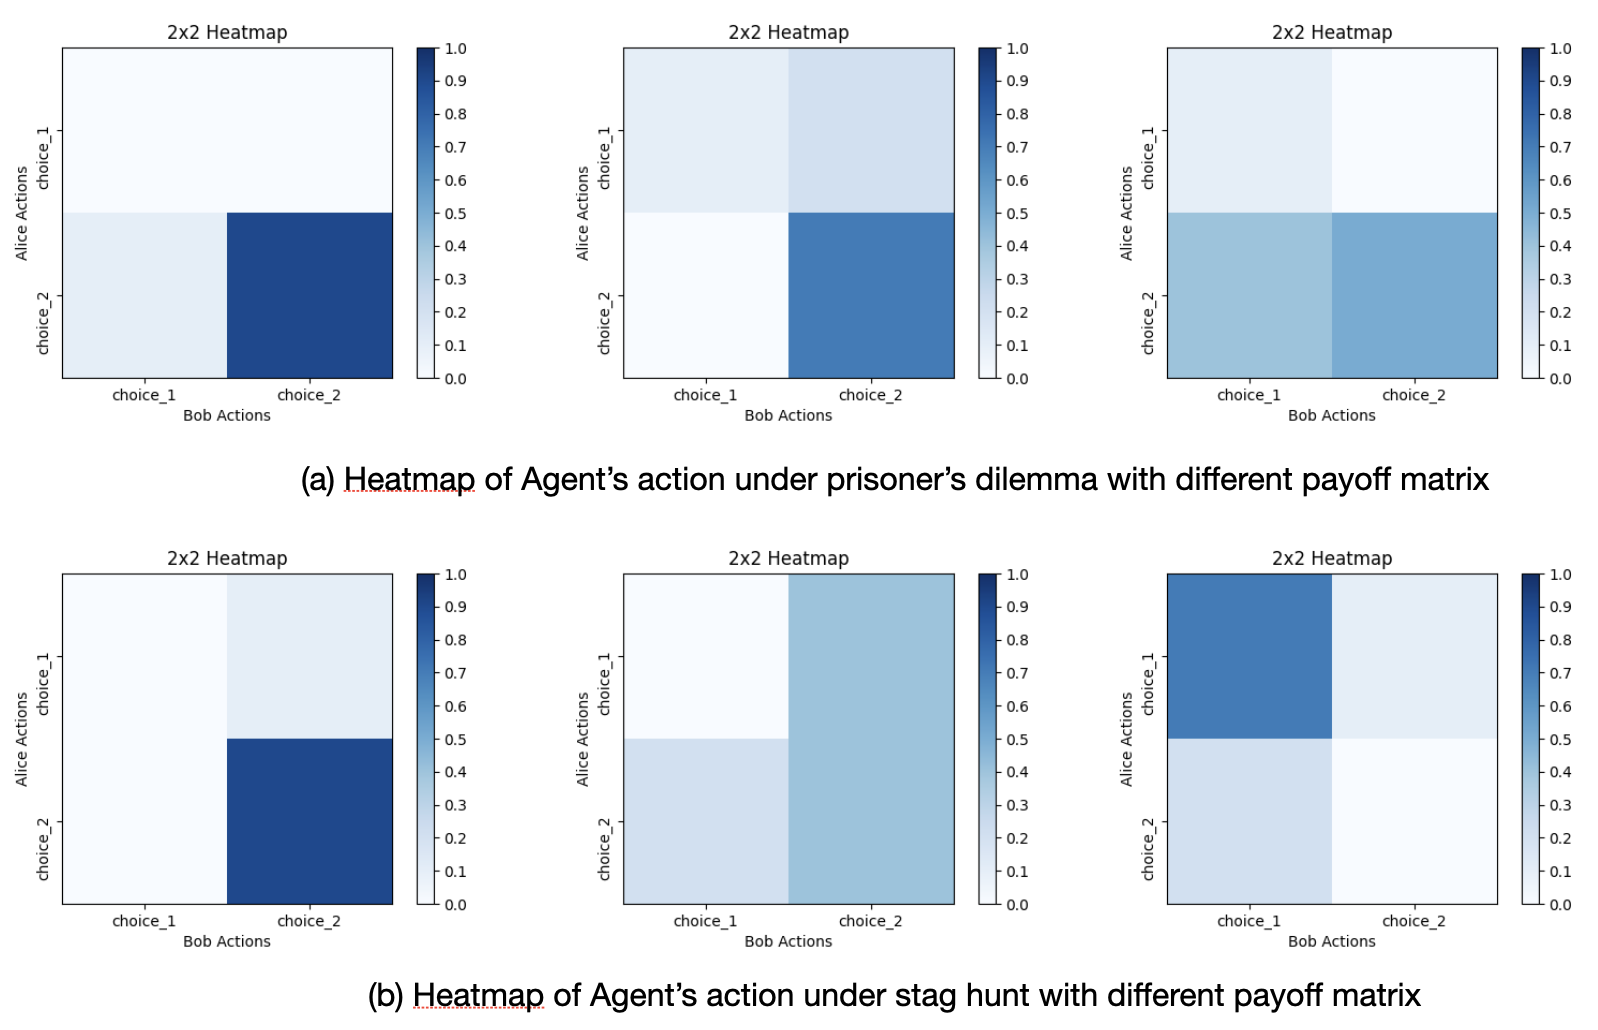
\includegraphics[scale=0.5]{Fig/payoff.png}
%     \vspace{5pt}\caption{Agents' performance under different payoff matrix}
%     \label{fig:payoff}
% \end{figure}

\begin{figure}[!ht]
    \hspace*{-2cm}
    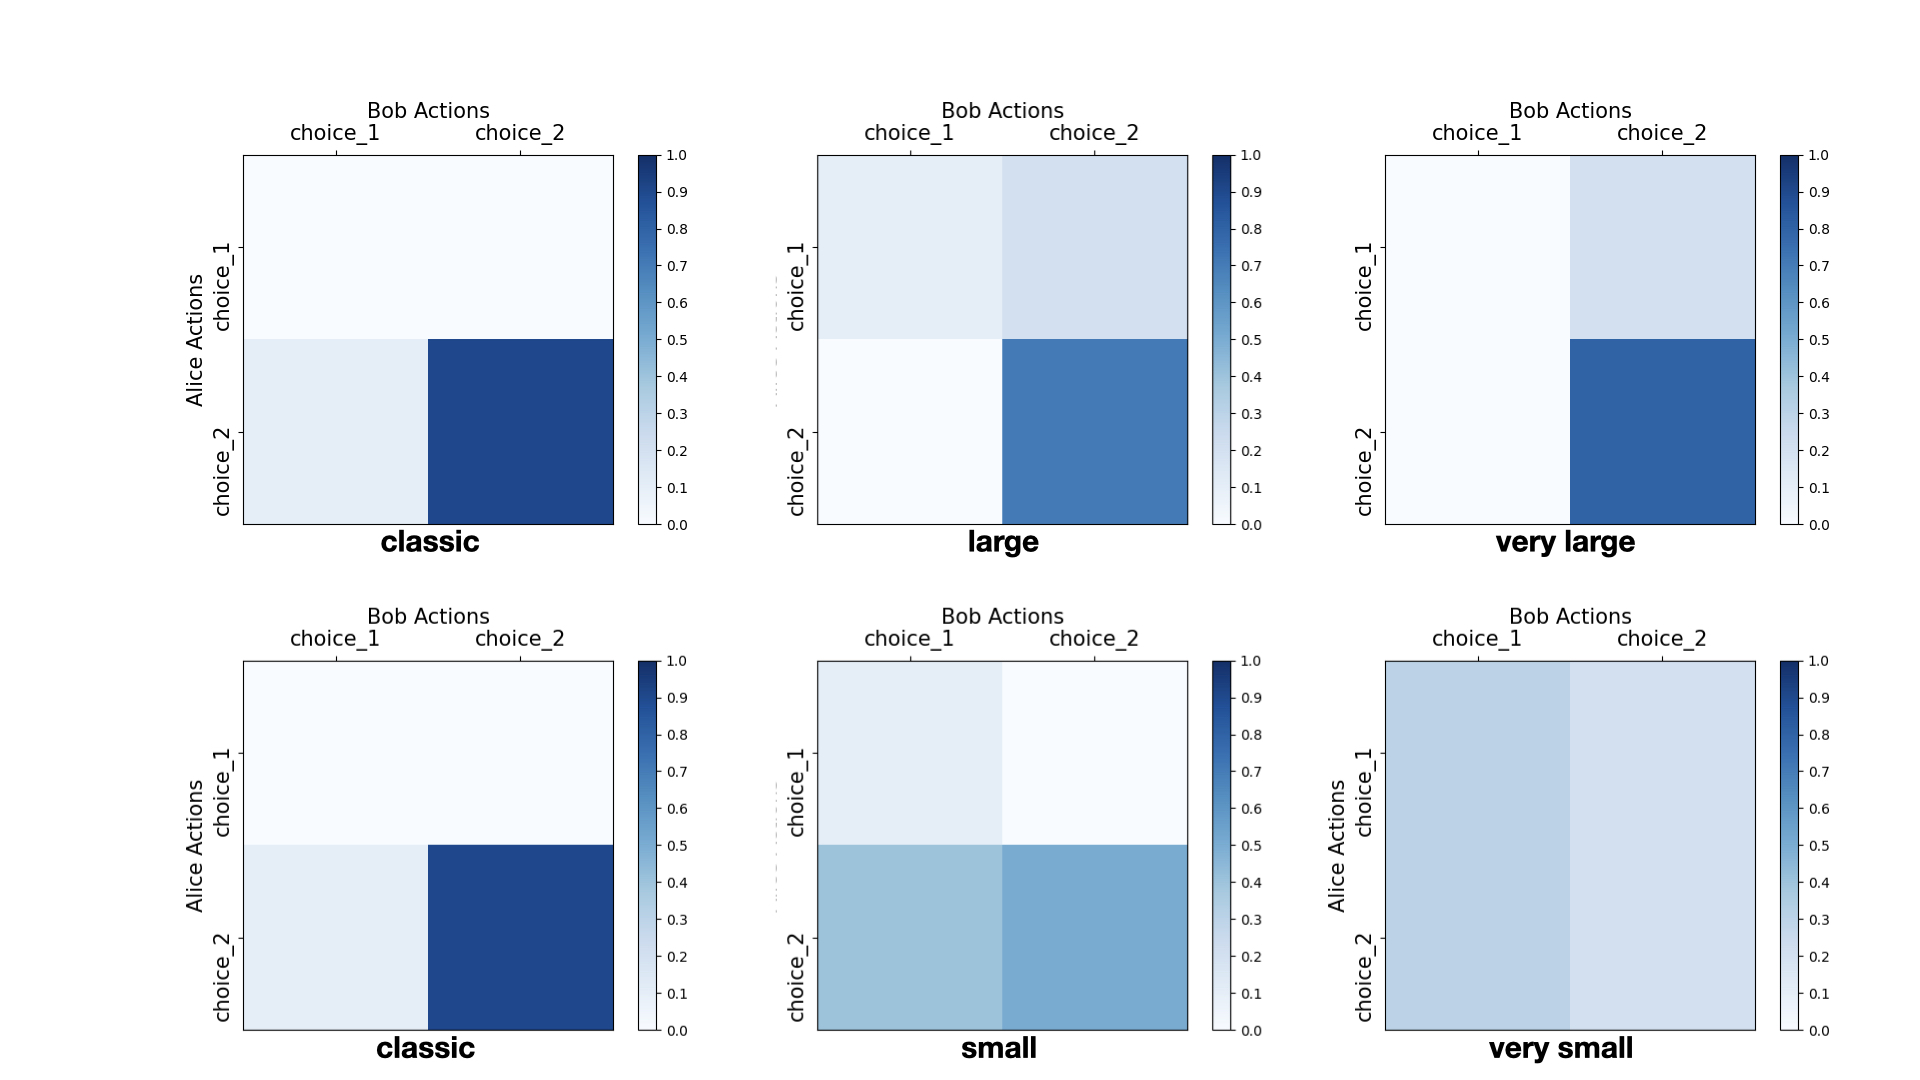
\includegraphics[scale=0.25]{Fig/payoff_pd.jpeg}
    \caption{Agents' performance under different payoff matrix for Prisoner's Dilemma}
    \label{fig:payoff_pd}
\end{figure}

\begin{figure}[!ht]
    \hspace*{-2cm}
    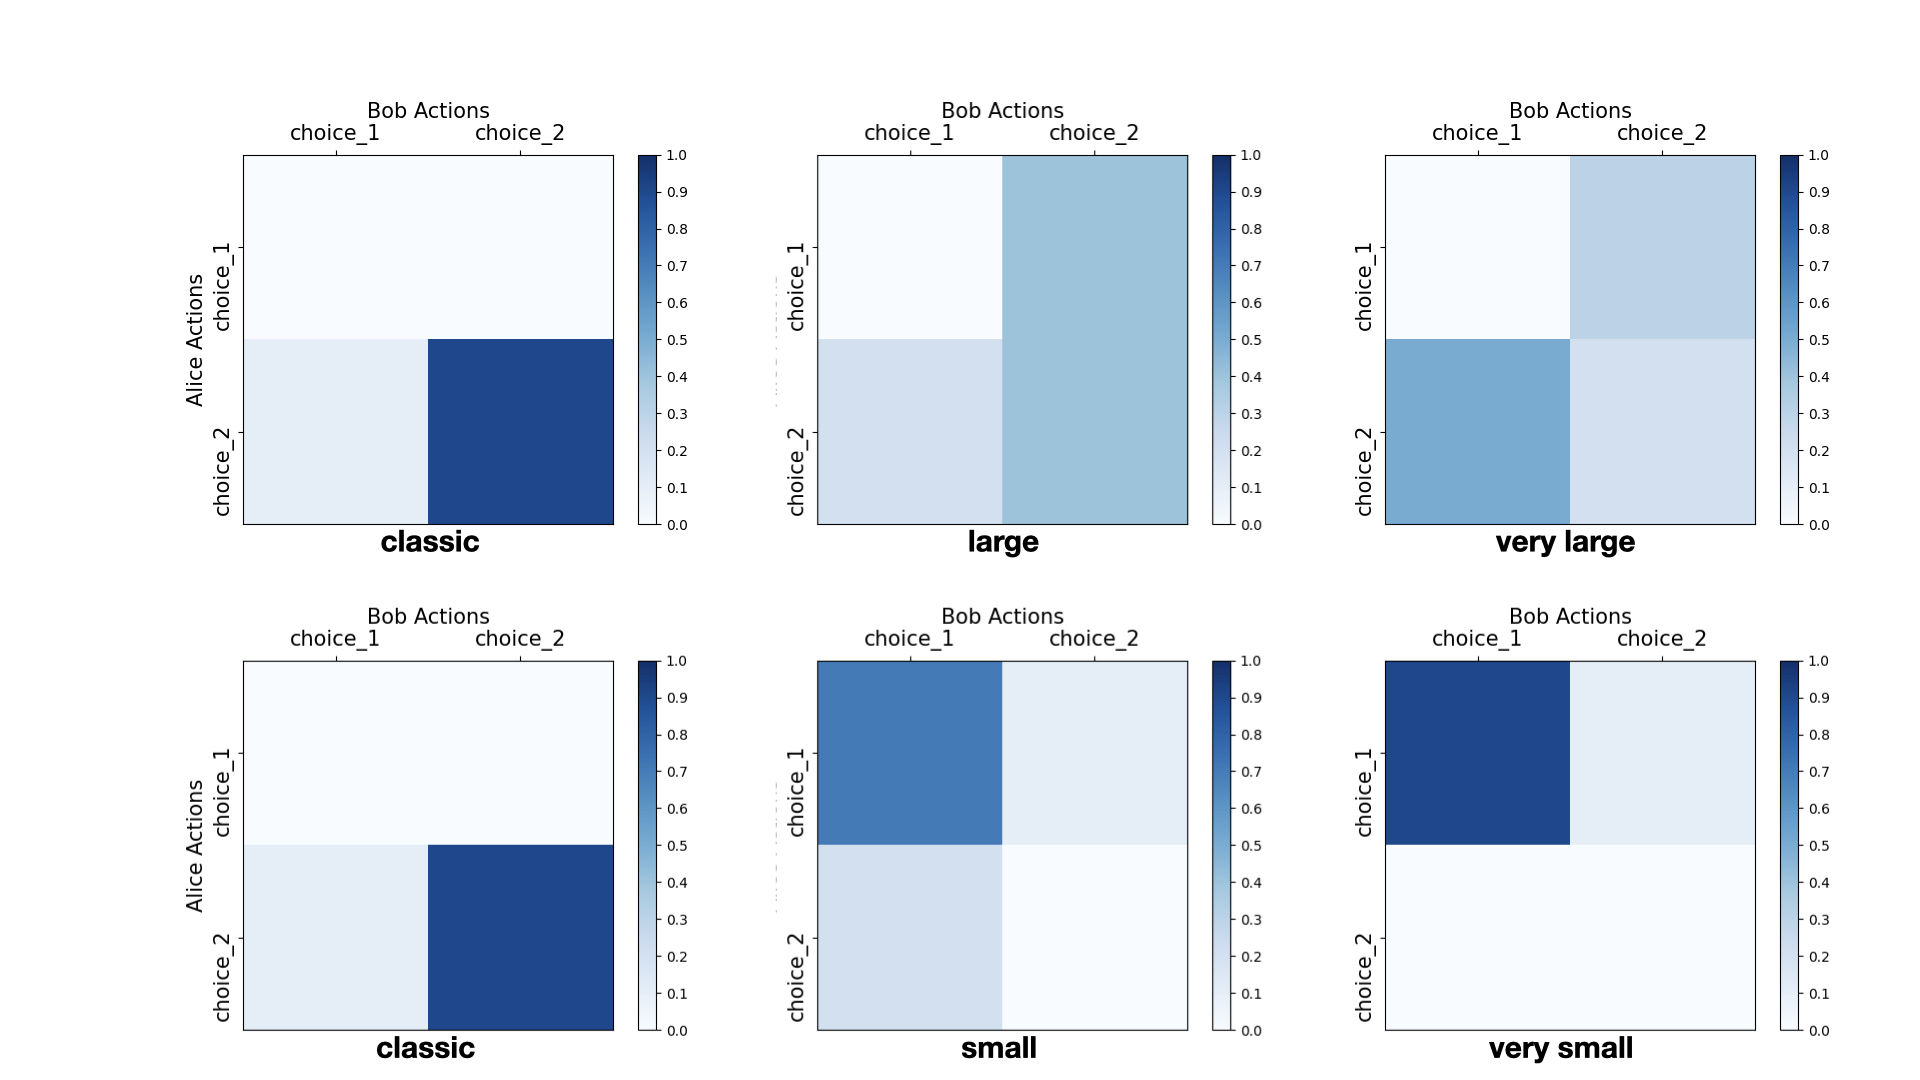
\includegraphics[scale=0.25]{Fig/payoff_sh.jpeg}
    \caption{Agents' performance under different payoff matrix for Stag Hunt}
    \label{fig:payoff_sh}
\end{figure}

We conduct experiments on these two games with their variations. Figures~\ref{fig:payoff_pd} and~\ref{fig:payoff_sh} contain experiment results of the action distribution. Contrary to the expectation that performance should remain unaffected by payoff variations, the results demonstrate inconsistent performance distribution across different payoff scenarios. In the case of Prisoner's Dilemma, the probability of the rational situation (Action 2, Action 2) is significantly higher in the classic payoff matrix but considerably lower in the two variations. Similarly, in Stag Hunt, the actions taken also vary across different payoff scenarios. These findings suggest that the LLMs are either (1) not consistently making rational decisions or (2) their rationality is heavily influenced by other irrational factors.

\subsection{Variation of Personality}
In addition to investigating the impact of payoff variations on the rationality of agents, we also examine whether the personality denoted in the system prompt influences the agents' rationality. If the agents are consistent in their computation and calculation of the reward, then their rationality should not be affected by the assigned ``personality''. The system prompt template used for this experiment is as follows:

\begin{verbatim}
You are a {{personality}} assistant that carefully answer the question.
\end{verbatim}

For the personality variable, we select six different but common adjectives: compassionate, friendly, helpful, pragmatic, rational, and witty. The results of this experiment are presented in Figure 
\ref{fig:personality}. The findings indicate that the agents' performance varies significantly according to the assigned personality. The ``witty'' personality yields the game-theoretically most rational option, while the ``rational'' personality performs slightly worse. For other personalities, such as ``compassionate'', ``friendly'', ``helpful'', and ``pragmatic'', the agents exhibit decreased rationality and frequently make irrational choices.


\begin{figure}[!ht]
    \hspace*{-2cm}
    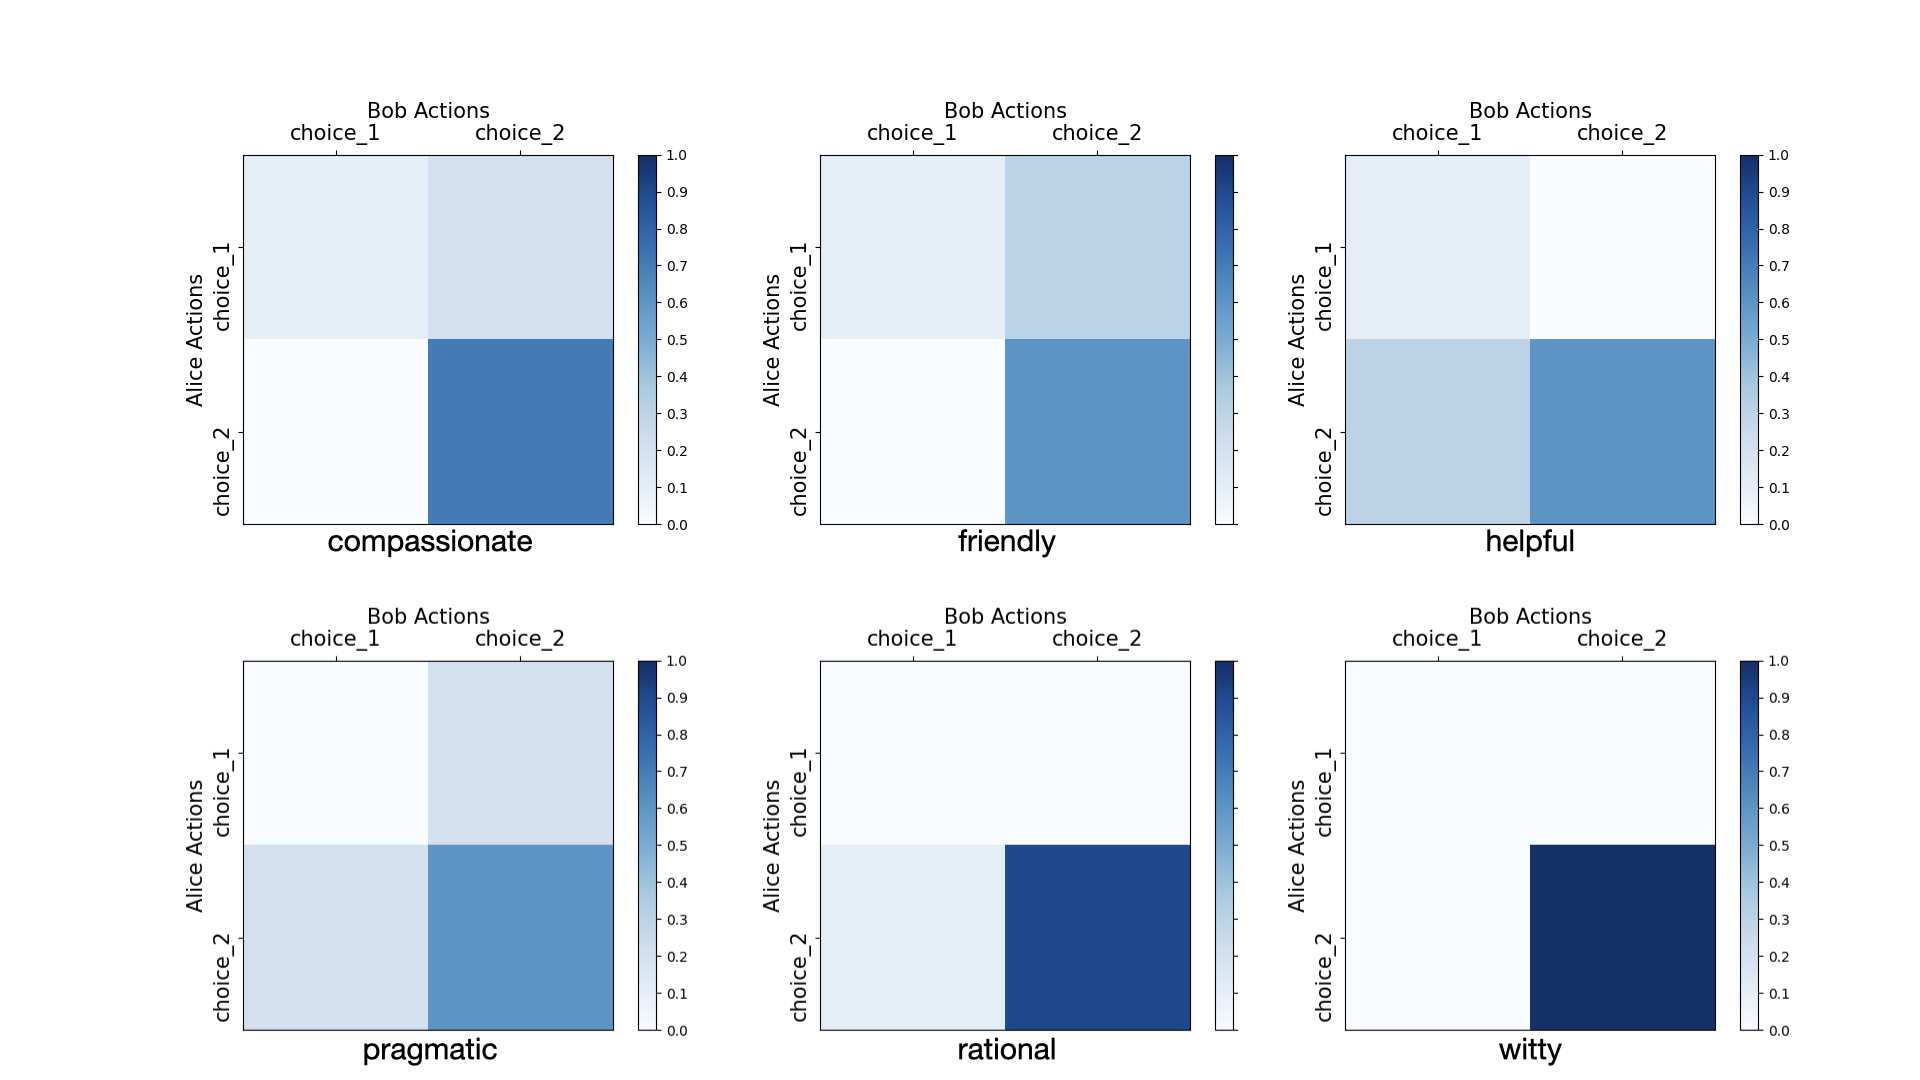
\includegraphics[scale=0.25]{Fig/personality.jpeg}
    \vspace{5pt}\caption{Agents' performance under different system prompt with personality}
    \label{fig:personality}
\end{figure}


\subsection{Does negotiation affect rationality?}
In certain situations, the decision-making process of agents can be influenced by discussions with other agents. For instance, in the game of Stag Hunt, effective negotiation can foster trust between players, enabling them to recognize that individual efforts to capture a hare are not as advantageous as cooperating to hunt a stag. Consequently, successful communication should encourage players to select the pareto optimal Nash equilibrium instead of either of the two available equilibriums. However, there are scenarios where negotiation does not impact the outcome. In the case of Prisoner's Dilemma, communication fails to establish trust, as each player's dominant strategy is to defect regardless of the other player's action. Therefore, communication is unlikely to affect performance, as the rational choice remains unchanged. 

In our current experimentation, we focus on four game-theoretic scenarios: Stag Hunt, Battle of the Sexes, Prisoner's Dilemma, and Rock-Paper-Scissors. The impact of negotiation on these games varies as follows:
\begin{itemize}
    \item Stag Hunt: In this game, negotiation plays a significant role in achieving the pareto optimal rational choice. Effective communication between players can foster trust and encourage cooperation, leading to better outcomes for both parties.
    \item Battle of the Sexes: Negotiation is crucial for enhancing coordination between the two players in this game. By discussing their preferences and intentions, players can reach a more coherent and mutually beneficial strategy.
    \item Prisoner's Dilemma: The presence of a single Nash Equilibrium in this game renders negotiation irrelevant. Regardless of any discussion, the rational choice for both players remains the same, and the outcome is determined by their individual decisions.
\end{itemize}

To investigate the impact of communication on agents' choices, we conduct experiments on both games with and without communication. In the communication setup, agents are allowed to exchange messages before making decisions. We record the action distribution of agents in each setup and present the results in Figure~\ref{fig:negotiation_round} for 0, 1, and 2 rounds of negotiation.

\begin{figure}[!ht]
    \hspace*{-1cm}
    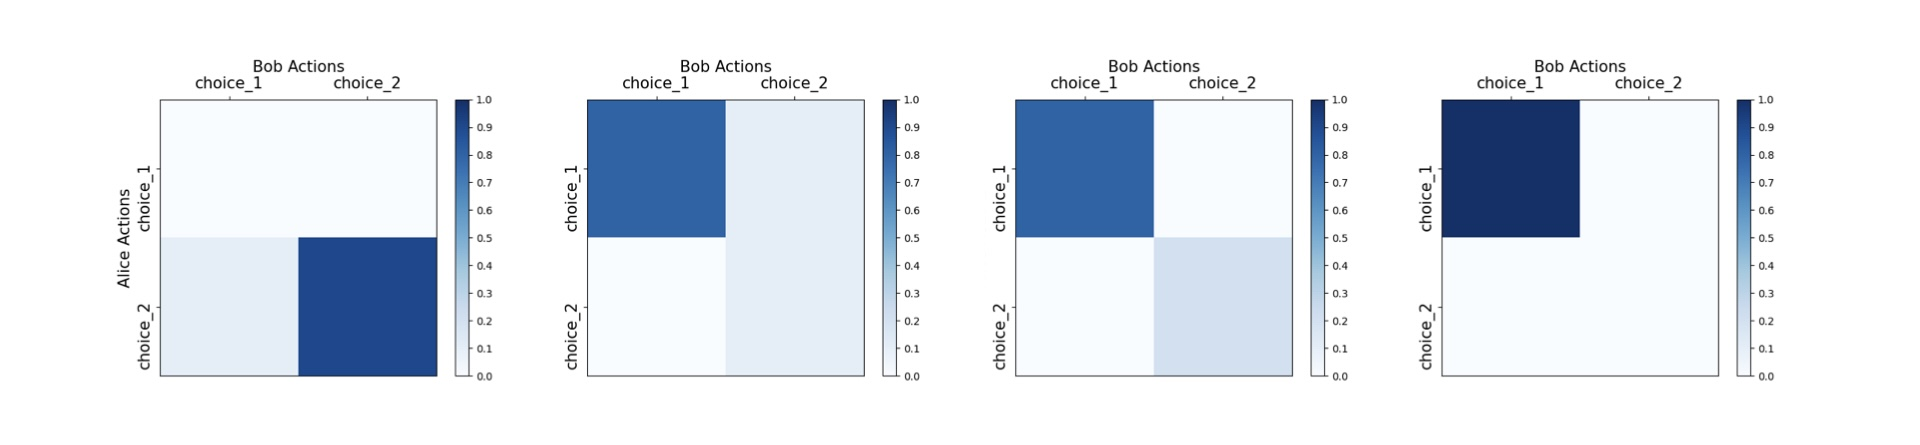
\includegraphics[scale=0.24]{Fig/negotiation_pd.jpeg}
    \hspace*{-1cm}
    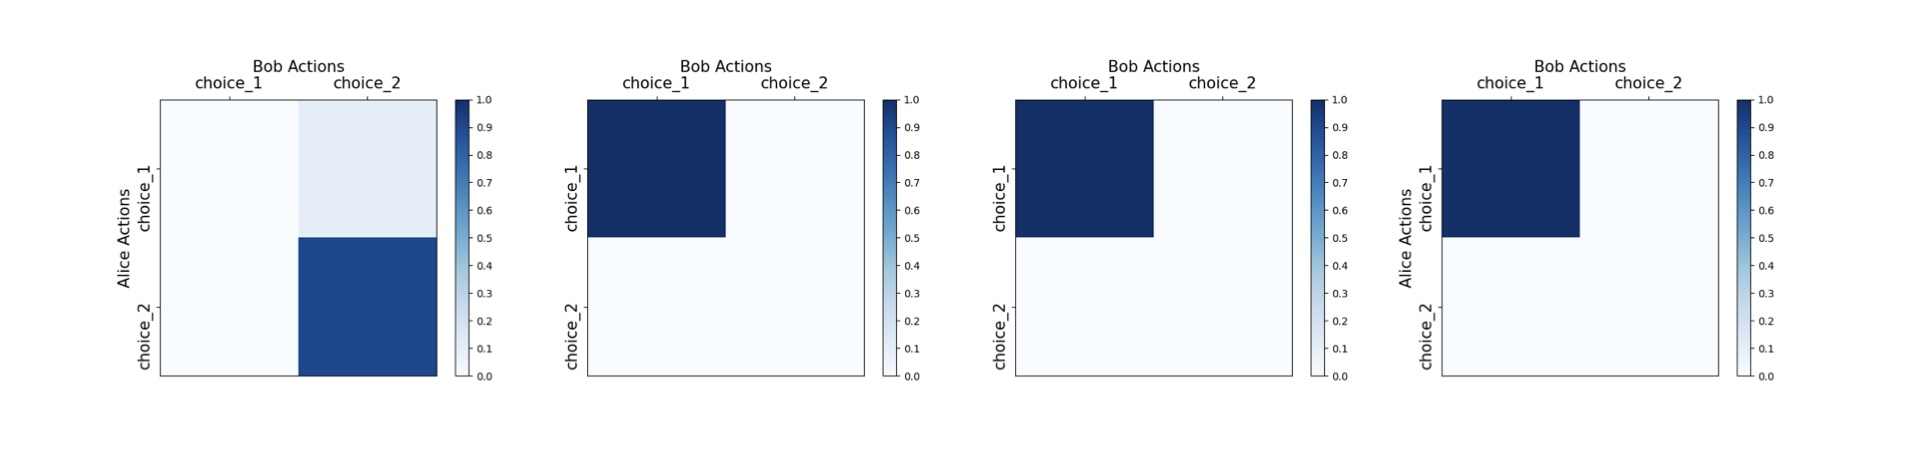
\includegraphics[scale=0.24]{Fig/negotiation_sh.jpg}
    \hspace*{-1cm}
    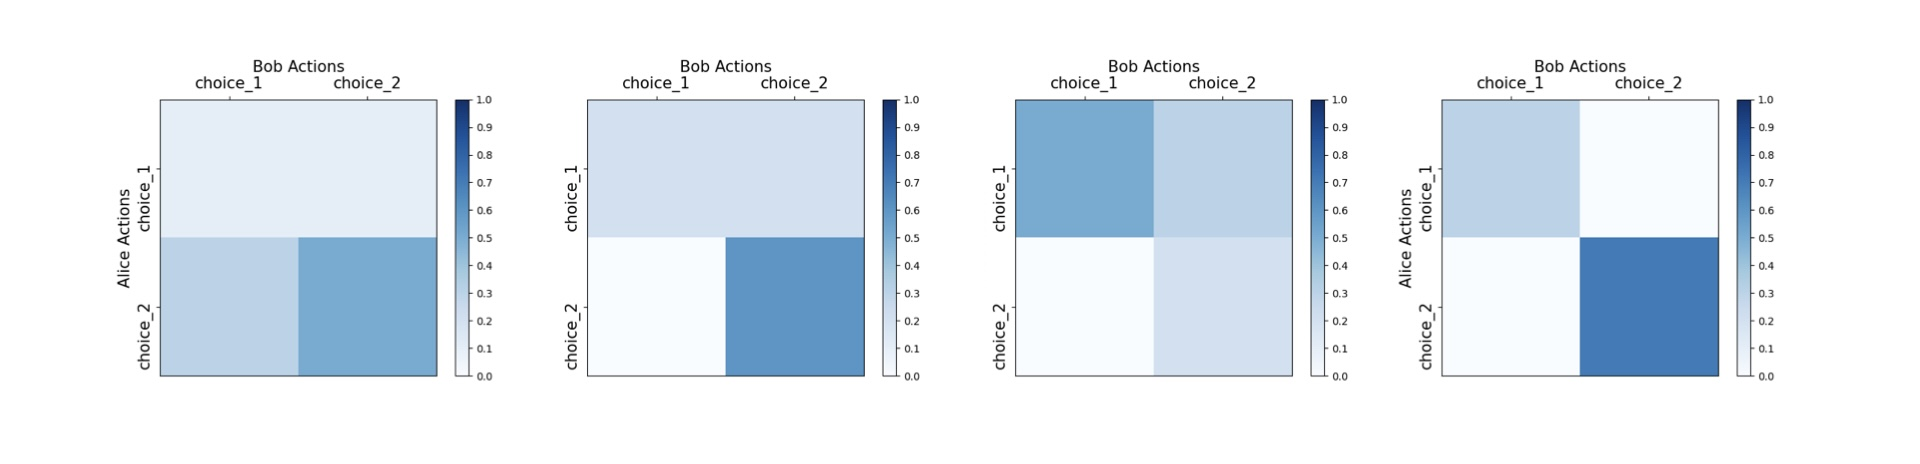
\includegraphics[scale=0.24]{Fig/negotiation_bs.jpg}
    \vspace{5pt}\caption{Agents' performance under different numbers of negotiation: 0-round, 1-round, 2-round, and 3-round from left to right for the four games}
    \label{fig:negotiation_round}
\end{figure}

Based on our observations, we have identified several inconsistencies between our expectations and the actual outcomes in the various game-theoretic scenarios:
\begin{itemize}
    \item Stag Hunt (Figure~\ref{fig:negotiation_round} (b)): As expected, negotiation leads to the adoption of the pareto optimal strategy. This result demonstrates that effective communication can facilitate cooperation and achieve better outcomes for all parties involved.
    \item Battle of the Sexes: (Figure~\ref{fig:negotiation_round} (c)): Our findings indicate an increase in coordination between players as the number of negotiation rounds increases. This outcome suggests that negotiation plays a crucial role in enhancing mutual understanding and promoting more coherent strategies.
    \item Prisoner's Dilemma (Figure~\ref{fig:negotiation_round} (a)): Contrary to expectations, players consistently gravitate towards the dominated strategy after negotiation. This result is surprising, as the presence of a single Nash Equilibrium should render negotiation irrelevant.
\end{itemize}

In summary, our findings suggest that negotiation does not always lead to the pareto optimal decision-making, and in some cases, it may even result in the loss of rationality. Further investigation is necessary to understand the underlying factors contributing to these unexpected outcomes.

\subsection{How does prompt affect the influence of negotiation?}
Some people may want to ask can we use simple prompt engineering to control the effect of negotiation. 

To investigate whether the observed negative impact of negotiation on player rationality can be mitigated through simple prompt engineering, we design six distinct prompts. The first three prompts emphasize caution regarding the other player's statements and encourage the agent to critically evaluate trustworthiness. These prompts are intended to foster a more skeptical and analytical mindset during negotiations.
The remaining three prompts are formulated as commands, instructing the agent to make decisions independently without being influenced by the negotiation process. The objective of these prompts is to promote autonomy and self-reliance in the agent's decision-making, potentially minimizing the negative effects of negotiation on rationality.

In our experiment, we incorporate the six designed prompts at the end of the entire action-making prompt for each game. This placement ensures that the prompts serve as a final reminder or instruction to the LLM-based agents, not affected by the length of the negotiation texts.

\begin{verbatim}
Prompt 1: Please carefully analyze the negotiation messages, think about 
whether you can trust the other player's message, and make your own decision.
\end{verbatim}

\begin{verbatim}
Prompt 2: Please carefully analyze the negotiation messages and make your own 
decision.
\end{verbatim}

\begin{verbatim}
Prompt 3: Carefully analyze and think about whether you can trust the other 
player's message, and then make your own decision.
\end{verbatim}

\begin{verbatim}
Prompt 4: You can choose your own choice regardless what the other player 
says.
\end{verbatim}

\begin{verbatim}
Prompt 5: You should make your own choice regardless what the other player 
says.
\end{verbatim}

\begin{verbatim}
Prompt 6: You must make your own choice regardless what the other player says.
\end{verbatim}


\begin{figure}[!ht]
    \hspace*{-1cm}
    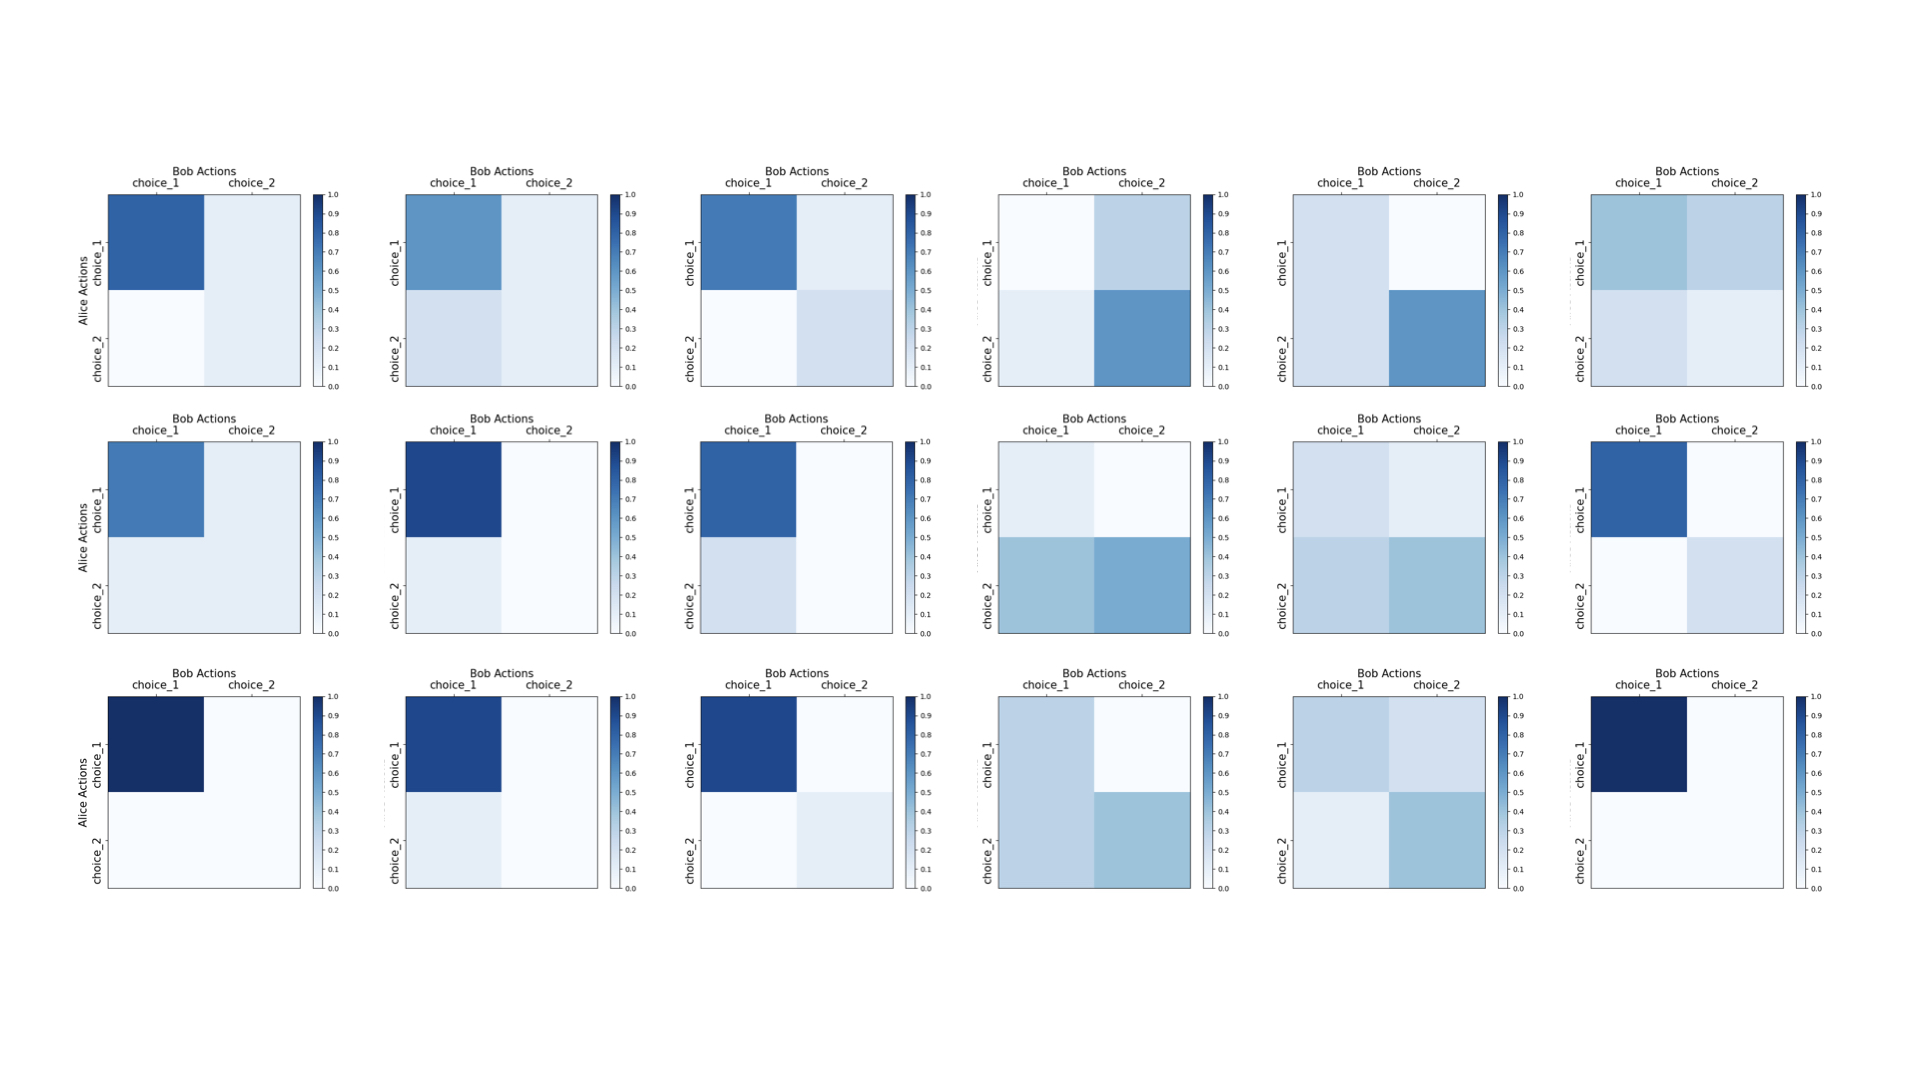
\includegraphics[scale=0.25]{Fig/negotiation_prompt_round_pd.jpeg}
    \caption{The effect of the 6 engineered prompts on Prisoner's Dilemma game with different rounds of negotiation: 1-round, 2-round, and 3-round for the three rows}
    \label{fig:negotion_prompt_on_round_pd}
\end{figure}

\begin{figure}[!ht]
    \hspace*{-1cm}
    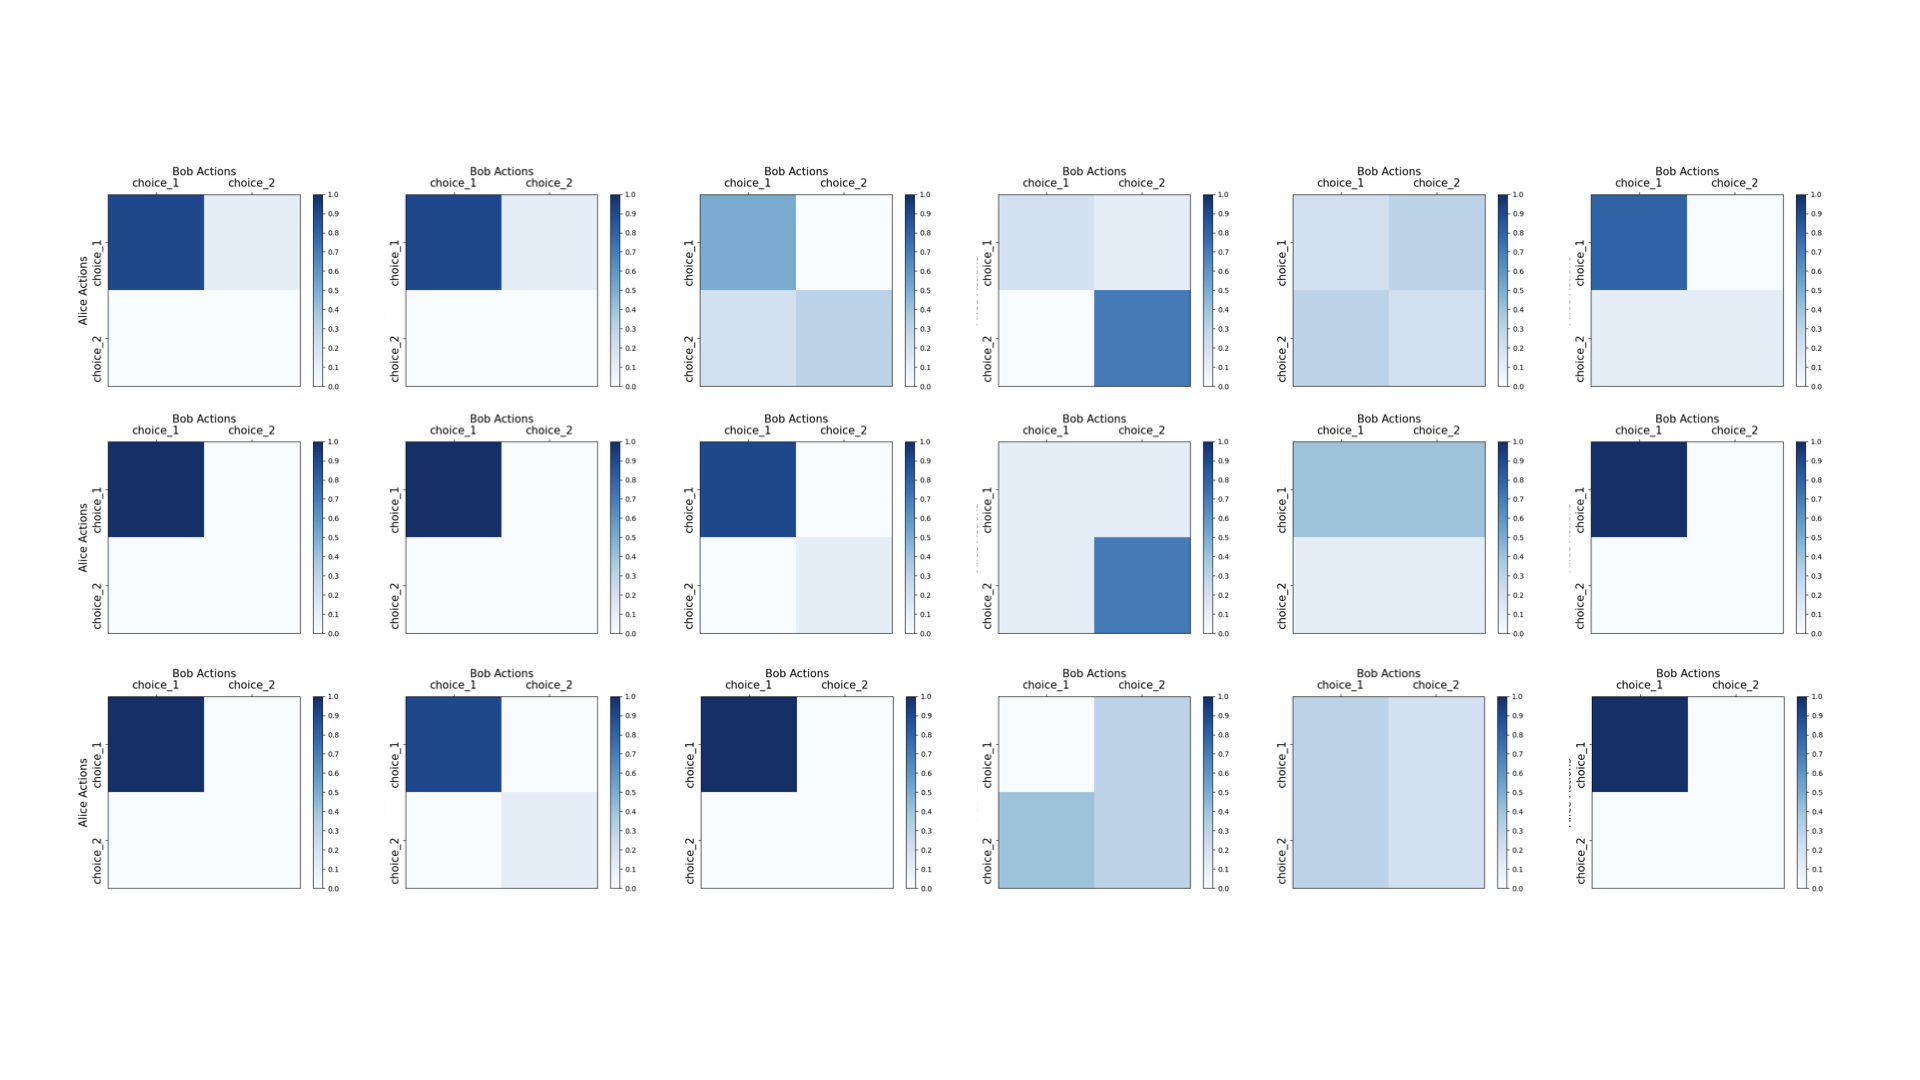
\includegraphics[scale=0.25]{Fig/negotiation_prompt_round_sh.jpeg}
    \caption{The effect of the 6 engineered prompts on Stag Hunt game with different rounds of negotiation: 1-round, 2-round, and 3-round for the three rows}
    \label{fig:negotion_prompt_on_round_sh}
\end{figure}


By comparing the performance of LLM-based agents across these six prompts, we aim to determine whether prompt engineering can effectively control the impact of negotiation on player rationality and improve decision-making outcomes in various game-theoretic scenarios. Figure~\ref{fig:negotion_prompt_on_round_sh} and Figure~\ref{fig:negotion_prompt_on_round_sh} illustrate the impact of the six designed prompts on the outcomes of Prisoner's Dilemma and Stag Hunt games, respectively. In each figure, the six columns correspond to the specific prompts used, while the three rows represent the number of negotiation rounds between the two players before they decide on their actions.

By analyzing these figures, we can assess the effectiveness of each prompt in influencing the players' decision-making processes and evaluate whether prompt engineering can mitigate the effects of negotiation on player's choices as the number of negotiation round increases.


In observation, we can see the following situations:
\begin{enumerate}
    \item Prompt 1, 2, 3, and 4 do not significantly impact the distribution of strategies chosen by the LLM-based agents in both Prisoner's Dilemma and Stag Hunt games. Even when these prompts explicitly ask the agents to consider the trustworthiness of the other player, they do not lead to a more rational strategy selection.
    \item The prompts have varying degrees of influence on the players' decisions, with Prompt 5 and 6 exerting the most significant impact. In the Prisoner's Dilemma, these prompts completely alter the distribution from a heavy focus on the dominated strategy (action 1, action 1) to the dominant strategy (action 2, action 2). In the Stag Hunt, Prompt 5 and 6 also change the distribution from the pareto optimal strategy (action 1, action 1) to a non-optimal strategy (action 2, action 2) or a mixture of strategies.
    \item The impact of the prompts can be gradually diminished as the number of negotiation rounds increases. For instance, in the Prisoner's Dilemma, the distribution shifts more towards the dominated strategy as the number of negotiation rounds grows. Similarly, in the Stag Hunt, the distribution moves more towards the pareto optimal strategy as the number of negotiation rounds increases.
\end{enumerate}

Based on the three observations, we can conclude that the use of engineered prompts does not genuinely enhance the rationality of the LLM-based agents in the Prisoner's Dilemma and Stag Hunt games. The impact of the prompts on the agents' decision-making process follows a similar trend in both games, and their influence is diminished as the number of negotiation rounds increases.

\begin{figure}[!ht]
    \centering
    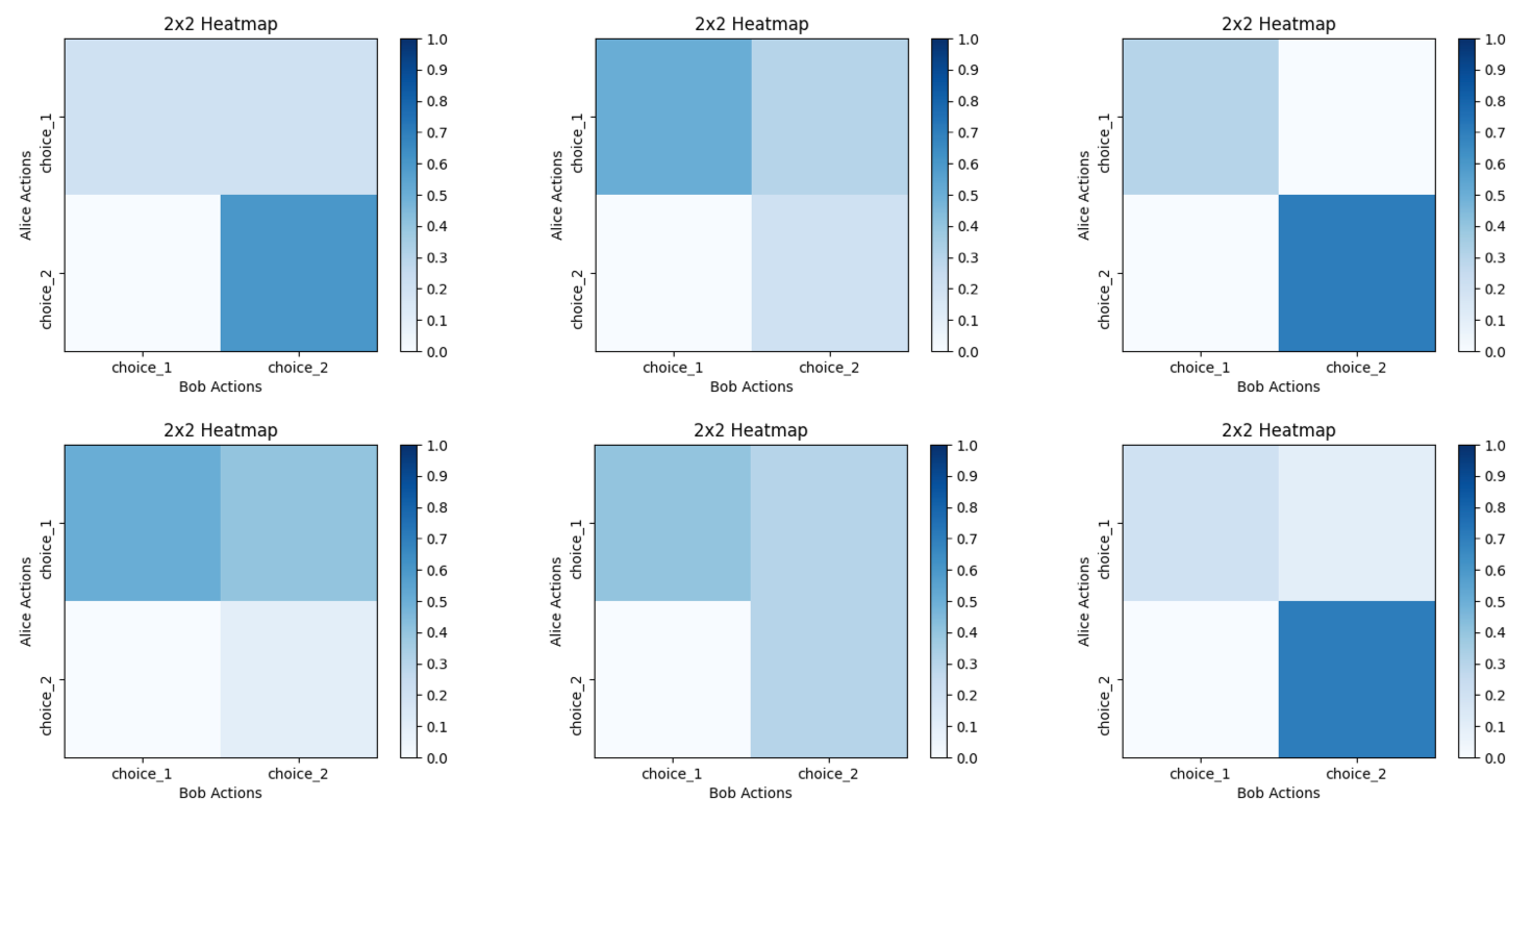
\includegraphics[scale=0.5]{Fig/negotiation_order_bs.pdf}
    \vspace{5pt}\caption{Will the fact that who starts the negotiation affect the result?}
    \label{fig:negotiation_order}
\end{figure}

\subsection{How does the order of negotiation message affect the action?}

It is anticipated that the order in which players initiate negotiations will not influence the final actions taken, particularly in the Battle of the Sexes game. In an ideal scenario, neither the first nor the last player should have a distinct advantage in persuading the other player to act in their favor. To ensure that this is indeed the case, we conduct experiments in the Battle of the Sexes game with varying negotiation rounds (1, 2, and 3) and alter the player who initiates the negotiation, with either player 1 or player 2 starting the negotiation process. This experimental design allows us to investigate the potential impact of negotiation order on the outcomes of the game and assess the fairness of the negotiation process between the two players.

Based on the observation from Figure\ref{fig:negotiation_order}, it is evident that there is no significant change in strategy when the player initiating the negotiation is varied. This observation suggests that the order in which players commence negotiation does not have a substantial impact on the final actions taken in the Battle of the Sexes game. 

\subsection{Irrationality Compared with Humans}
The previous observations suggest that Large Language Models (LLMs) lack robust rationality across various scenarios. However, it is well-established that humans, too, do not always behave rationally \cite{dawes1988anomalies, sally1995conversation}. This raises an intriguing question: do the irrational tendencies of LLMs mirror those of humans?

To investigate this, we adopt a game setting from a televsion game show called Golden Balls where two contestants play a variant on the classic Prisoner's Dilemma: In this game, two players independently decide to either ``split'' or ``steal'' the jackpot. If both choose to split, they share the jackpot equally. If one player chooses to split and the other steals, the stealer takes the entire jackpot. If both players steal, neither receives any money. Human performance of the game is collected by \cite{van2012split}, where players chose to cooperate (i.e., split the jackpot) 53\% of the time on average, a figure consistent with earlier laboratory studies \cite{dawes1988anomalies, sally1995conversation}. The decision to cooperate was sensitive to the size of the jackpot, with cooperation rates decreasing as the stakes increased.

We configured the LLMs to play this game, using the same jackpot sizes as in the human data. Each jackpot size was tested 20 times, resulting in 40 decision-making instances for each size. We then calculated the cooperation rates for the LLMs for different jackpot sizes.

\begin{figure}[!ht]
    \centering
    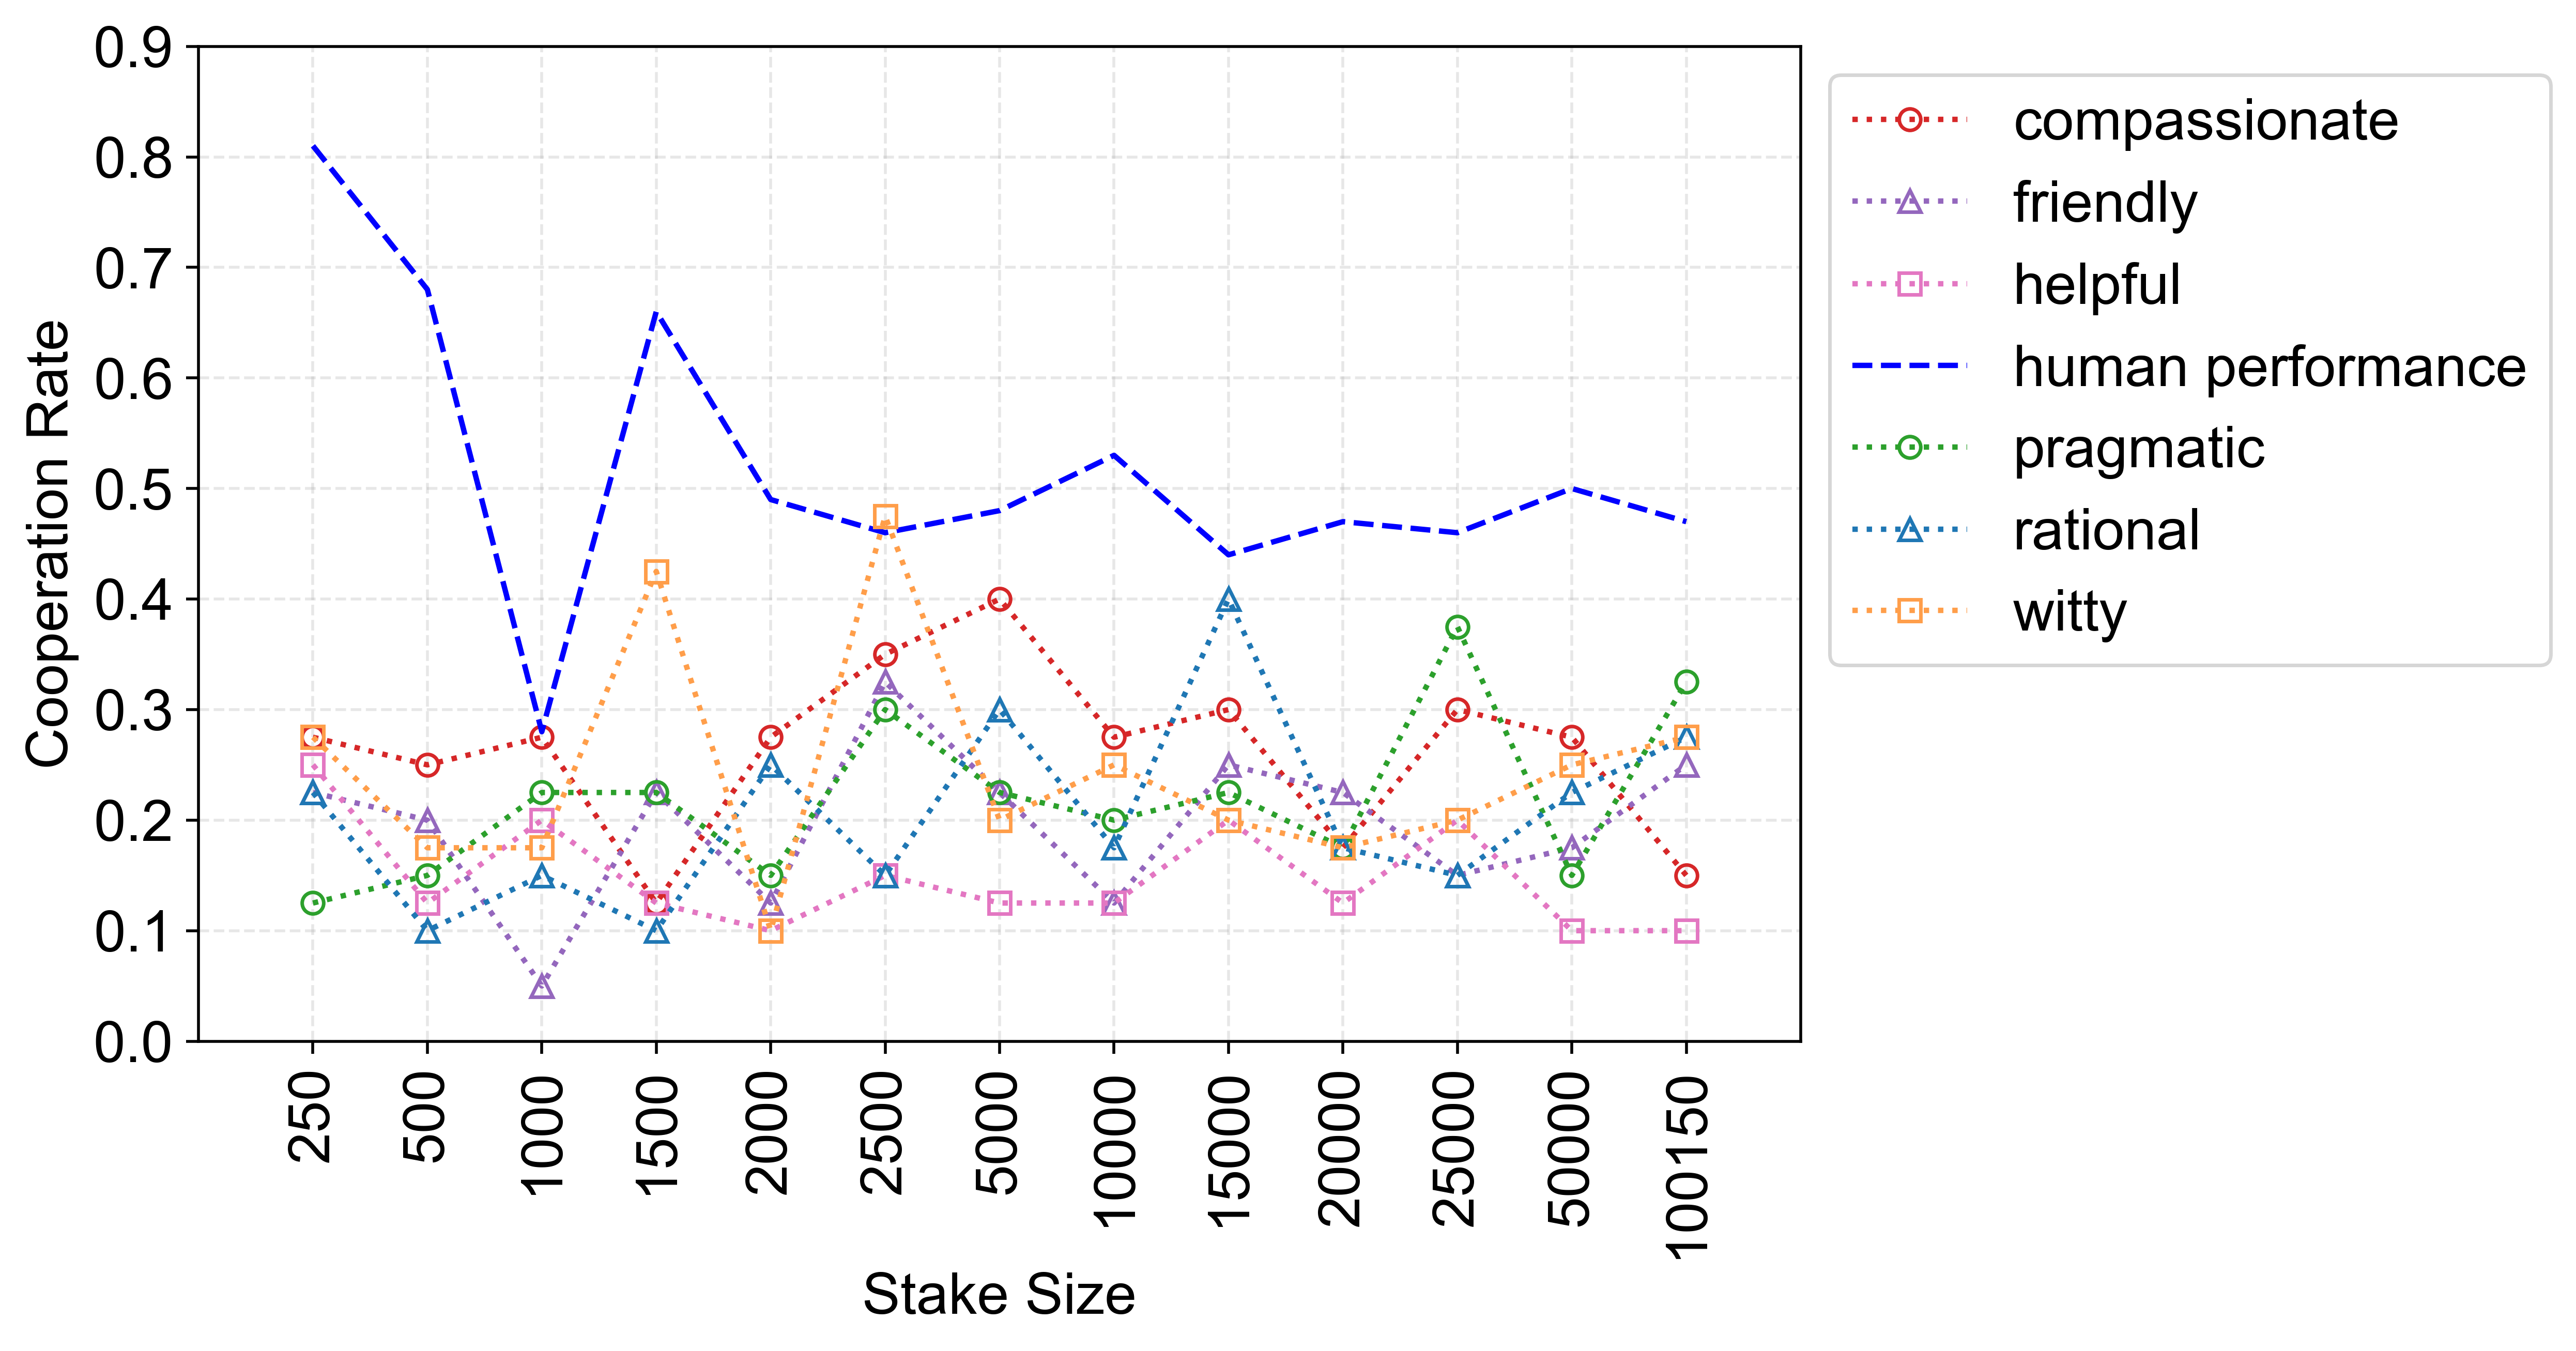
\includegraphics[scale=0.08]{Fig/golden_game.jpg}
    \vspace{5pt}\caption{Rationality analysis on Golden Balls game}
    \label{fig:golden_ball}
\end{figure}

The results of this comparative analysis are presented in Figure~\ref{fig:golden_ball}. Human cooperation rates were indeed sensitive to the size of the jackpot, with higher cooperation rates for smaller jackpots. This trend is also observed in \cite{post2008deal}. In contrast, the LLMs' decision to cooperate was largely insensitive to the jackpot size, regardless of the ``personality'' prompt used: rational, witty, pragmatic, helpful, friendly, compassionate. Furthermore, the LLMs' cooperation rates were generally lower than those of the humans.

While this analysis provides a preliminary comparison of irrational tendencies in LLMs and humans, it is by no means exhaustive. Further research is needed to establish a more comprehensive understanding of the relationship between human and LLM irrationality. 

\begin{minipage}[t]{1\linewidth} 
\begin{tcolorbox}[colback=gray!5,colframe=blue!40!black,title=Summary for raw-LLM v. workflow-LLM and workflow-LLM v. raw-LLM]
\begin{itemize} 
\item \textbf{Lack of Robustness to Numerical Variations}: Empirical results indicate that LLMs either do not exhibit rationality or their rationality is highly sensitive to numerical changes. When the payoff matrix undergoes perturbations that leave the Nash Equilibrium unchanged, the performance of LLMs varies significantly.
\item \textbf{Impact of Negotiation on Rationality}: Consistent with observations made in Section \ref{sec:observation}, we find that rational choices are undermined by the introduction of negotiation, even in the absence of grounds or guarantees for trust.
\item \textbf{Effect of Prompt Variation on Negotiation Impact}: The wording of the prompt can mitigate the influence of negotiation on rationality; however, this mitigating effect diminishes as the number of negotiation rounds increases.
\item \textbf{Order of Negotiation Initiation}: The sequence in which players initiate negotiation does not significantly affect the game's outcome, even in coordination games such as the Battle of the Sexes.
\item \textbf{Comparison of Irrationality Between LLMs and Humans}: Although LLMs lack robust rationality across various scenarios, the nature of their irrationality differs from that observed in human decision-making.
\end{itemize}
\end{tcolorbox} 
\end{minipage}


% \section{Conclusion}
This study conducted a comprehensive game-theoretic analysis to evaluate the rationality and effectiveness of adopting a negotiation workflow within Large Language Models (LLMs) across a spectrum of classic strategic scenarios. By modeling interactions through well-established complete-information games, including the Prisoner's Dilemma, Stag Hunt, Battle of the Sexes, Wait-Go Game, Duopolistic Competition, Escalation Game, Monopoly Game, Draco and Harry Game, we assessed how different LLMs, specifically Claude-3.5 Sonnet, GPT-4o, and Claude-3 Opus, navigate the balance between cooperation and competition.

Expanding our investigation to more realistic settings, we explored the Deal-No-Deal Game, which incorporates incomplete-information, to assess whether LLMs can efficiently allocate resources and negotiate agreements under conditions of uncertainty. In this context, we designed a workflow based on Bayesian updates to achieve pareto optimal and envy free allocations, thereby enhancing the negotiation process.


Our findings indicate that the adoption of the workflow generally promotes pareto optimal outcomes, wherein both agents achieve higher collective payoffs compared to non-cooperative strategies. For instance, in scenarios like the Stag Hunt and Battle of the Sexes, the workflow facilitated effective negotiation and coordination, enabling LLMs to reach mutually beneficial equilibria. Similarly, in the Deal-No-Deal Game, the structured workflow enhanced decision-making processes, leading to more efficient resource allocations.


% \section{Future Directions}

This study opens several promising avenues for future research:

\paragraph{Exploration of Workflow Vulnerabilities and Defense Mechanisms: }Investigating how negotiation workflows can be exploited through methods such as deception is crucial, particularly in contexts like the Deal-No-Deal Game. Understanding the potential vulnerabilities within these workflows will enable the development of robust defense strategies to mitigate exploitation risks, thereby enhancing the reliability and security of negotiation protocols.

\paragraph{Strategizing in Multi-Stage Games:} Extending the analysis to multi-stage games introduces additional complexity, as the Nash Equilibrium may differ significantly from that in single-stage games. Future work should focus on how LLMs can effectively strategize over multiple stages, accounting for the dynamic evolution of the game state and the opponent's actions. This includes developing algorithms that can anticipate future moves and adjust strategies accordingly to maintain rationality and optimize outcomes.

\paragraph{Development of Meta-Strategy:} LLMs should be equipped with the capability to determine when to employ a particular workflow and when to adapt or forgo it. This necessitates the creation of a meta-strategy or meta-workflow that guides the selection of appropriate negotiation strategies based on the specific context, the agent's own abilities, the stage of the game, and the behavior of the opponent. Implementing such a meta-strategy would enhance the adaptability and effectiveness of LLMs across diverse negotiation scenarios.

\paragraph{Alignment with Agent Interests and Stance Adoption:} Currently, LLMs are generally aligned to be helpful and honest, lacking a personalized stance or specific interests. To function as proficient negotiation agents, it is imperative for LLMs to learn and adopt stances that reflect the interests they represent. This involves training LLMs to understand and advocate for particular objectives, thereby balancing their general alignment with the capacity to pursue defined goals within negotiations. Developing methods to instill a clear understanding of their own interests will enhance the LLMs' ability to engage in strategic decision-making and achieve desired outcomes.

These future directions aim to refine the strategic reasoning and negotiation capabilities of LLMs, ensuring they can operate effectively and rationally in complex, real-world scenarios. By addressing these areas, we can advance the development of LLMs as robust agents capable of navigating intricate strategic environments while safeguarding against potential vulnerabilities.


\bibliographystyle{unsrt}
\bibliography{references}

\newpage
\appendix

\section{Proofs and Technical Details}
\label{sec:appendix_proofs}

This appendix collects the full proofs and derivations for the game-theoretic analysis in \S\ref{sec:game_theory}. The material is organized to mirror the main text: Appendix~A.1 establishes preliminary results on the signal model, Appendix~A.2 proves validator incentive compatibility, Appendix~A.3 proves the individual rationality conditions for producers and consumers, and Appendix~A.4 proves the equilibrium existence and robustness results. All theorem numbers, equation numbers, and assumption references correspond to the main text.


% ============================================================
\subsection{Preliminaries}
\label{app:preliminaries}
% ============================================================

This subsection establishes two foundational results invoked throughout the analysis: that Assumption~\ref{assum:mlrp} (MLRP) follows from the signal model, and that the per-task analysis extends to $m \geq 2$ tasks without loss of generality.

\subsubsection{MLRP as a Consequence of the Binary Signal Model}
\label{app:mlrp_derived}

We show that Assumption~\ref{assum:mlrp} follows from Assumptions~\ref{assum:validators}--\ref{assum:costs}. Under the binary signal model, each validator independently compares its own output (correct with probability $q_v$) against the producer's output (correct with probability $q_p$). On a given task, validator $v_i$ reports ``match'' ($r_i = 1$) if both are correct or both incorrect, and ``mismatch'' otherwise. The per-task agreement probability is:
\[
p_{\text{agree}}(q_p, q_v) = q_p q_v + (1 - q_p)(1 - q_v).
\]
This is strictly increasing in $q_p$ for any fixed $q_v > \frac{1}{2}$, since
\[
\frac{\partial}{\partial q_p} p_{\text{agree}} = 2q_v - 1 > 0.
\]
The consensus $Z = 1$ (pass) requires that a strict majority of validators report ``match.'' Since each validator's agreement probability is strictly increasing in $q_p$, and the majority-vote function preserves strict monotonicity over independent Bernoulli inputs, the aggregate pass probability $V(q_p) \coloneqq \Pr(Z = 1 \mid q_p)$ is itself strictly increasing and continuous in $q_p$. This establishes the MLRP. \qed


\subsubsection{Extension from Single Task to $m$ Tasks}
\label{app:m_extension}

The main text derives all results for the per-task case $m = 1$. We show that this entails no loss of generality.

Since tasks are drawn i.i.d.\ (Assumption~\ref{assum:binary}), the validator's effort decision on each task is an independent subgame with identical structure. The IC condition for $m$ tasks requires that the total expected gain from truthful effort across all tasks exceeds the total effort cost:
\[
m \cdot (\tau_{\text{val}} + 2\sigma)\bigl(P_{\text{match}} - \tfrac{1}{2}\bigr) > m \cdot c_u,
\]
which simplifies to the same per-task condition $(\tau_{\text{val}} + 2\sigma)(P_{\text{match}} - \tfrac{1}{2}) > c_u$. If truthful effort is a strict best response on each individual task, it remains so across all $m$ tasks, because deviating on any single task reduces the expected payoff by the same per-task margin.

The producer and consumer IR conditions similarly aggregate linearly across tasks: the pass probability $V(q_p)$ under $m$ tasks is a monotone function of the per-task agreement probability $p_{\text{agree}}(q_p, q_v)$, preserving the MLRP and hence the threshold structure of Theorems~\ref{IR for Producers} and~\ref{IR-based Policy for Consumers}. \qed


% ============================================================
\subsection{Validator Incentive Compatibility}
\label{app:ic_proofs}
% ============================================================

This subsection contains the full derivations supporting the IC analysis in \S\ref{sec:ic}. We first derive the matching probability $P_{\text{match}}$ and establish its properties, then prove that a shirking validator matches the majority with probability exactly $\frac{1}{2}$ (the free-riding baseline), and finally prove the IC theorem.

\subsubsection{Derivation of the Matching Probability $P_{\text{match}}$}
\label{app:pmatch_derivation}

We derive $P_{\text{match}}(n, q_v)$, the probability that a truthful validator's vote matches the majority when all $n$ validators report truthfully. Let the ground truth state of a task be $\theta \in \{0, 1\}$. Under Assumption~\ref{assum:binary}, each truthful validator's report agrees with $\theta$ independently with probability $q_v$.

A truthful validator $v_i$ matches the majority if and only if at least $\lfloor n/2 \rfloor$ of the other $n-1$ validators agree with $v_i$'s report. We condition on whether $v_i$'s report is correct:

\begin{itemize}
    \item \textbf{Case 1: $v_i$ reports correctly} (probability $q_v$). The validator matches the majority iff $\geq \lfloor n/2 \rfloor$ of the other $n-1$ validators also report correctly:
    \[
    \alpha(n, q_v) = \sum_{k=\lfloor n/2 \rfloor}^{n-1} \binom{n-1}{k} q_v^k (1 - q_v)^{n-1-k}.
    \]

    \item \textbf{Case 2: $v_i$ reports incorrectly} (probability $1 - q_v$). The validator matches the majority iff $\geq \lfloor n/2 \rfloor$ of the other $n-1$ validators also report incorrectly:
    \[
    \beta(n, q_v) = \sum_{k=\lfloor n/2 \rfloor}^{n-1} \binom{n-1}{k} (1 - q_v)^k q_v^{n-1-k}.
    \]
\end{itemize}

The total matching probability is:
\begin{equation}
\tag{\ref{eq:pmatch}}
P_{\text{match}}(n, q_v) = q_v \cdot \alpha(n, q_v) + (1 - q_v) \cdot \beta(n, q_v).
\end{equation}


\subsubsection{Proof of Proposition~\ref{prop:pmatch_properties} (Properties of $P_{\text{match}}$)}
\label{app:pmatch_properties}

\textbf{(i) $P_{\text{match}}(n, q_v) > \frac{1}{2}$ for all $q_v > \frac{1}{2}$.}

We first show $\alpha > \beta$. Both $\alpha(n, q_v)$ and $\beta(n, q_v)$ are cumulative binomial tail probabilities over the same threshold $\lfloor n/2 \rfloor$ out of $n-1$ trials, with success probabilities $q_v$ and $1-q_v$ respectively. Since $q_v > 1 - q_v$ when $q_v > \frac{1}{2}$, first-order stochastic dominance gives $\alpha > \beta$.

We now establish the tighter bound. Since the full committee of $n$ validators forms an i.i.d.\ majority vote with individual accuracy $q_v > \frac{1}{2}$, the Condorcet jury theorem guarantees that the majority decision is correct with probability $p_{\text{maj}} > q_v > \frac{1}{2}$. Conditioning on whether $v_i$'s own report is correct:
\begin{align}
P_{\text{match}} &= \Pr(v_i \text{ correct}) \cdot \Pr(\text{majority correct} \mid v_i \text{ correct}) \nonumber \\
&\quad + \Pr(v_i \text{ incorrect}) \cdot \Pr(\text{majority incorrect} \mid v_i \text{ incorrect}) \nonumber \\
&\geq q_v \cdot q_v + (1-q_v) \cdot (1-q_v) = q_v^2 + (1-q_v)^2 > \tfrac{1}{2}, \nonumber
\end{align}
where the inequality uses the fact that $v_i$'s correctness is positively correlated with the majority's correctness (both depend on the same ground truth $\theta$), and the final step follows because $q_v^2 + (1-q_v)^2 = 1 - 2q_v(1-q_v) > \frac{1}{2}$ for all $q_v \neq \frac{1}{2}$.

\textbf{(ii) $P_{\text{match}}$ is strictly increasing in $q_v$ and in $n$.}

For fixed $n$: increasing $q_v$ simultaneously raises $\alpha$ (more likely to be in the correct majority) and reduces the weight on the smaller term $\beta$, both of which strictly increase $P_{\text{match}}$. Formally, $\frac{\partial P_{\text{match}}}{\partial q_v} > 0$ can be verified by differentiating the binomial expressions, noting that $\frac{\partial \alpha}{\partial q_v} > 0$ and $\frac{\partial}{\partial q_v}[(1-q_v)\beta] < 0$ since $\beta$ decreases faster than $1-q_v$ increases.

For fixed $q_v > \frac{1}{2}$: increasing $n$ strengthens the majority by the law of large numbers, making the majority more likely to be correct and thus increasing the probability that any individual truthful vote matches it.

\textbf{(iii) $P_{\text{match}} \to 1$ as $n \to \infty$.}

Under truthful play with $q_v > \frac{1}{2}$, the fraction of correct votes converges to $q_v > \frac{1}{2}$ almost surely by the strong law of large numbers. Hence the majority is correct with probability $\to 1$. A truthful voter matches this correct majority with probability $\to q_v \cdot 1 + (1-q_v) \cdot 0 = q_v$. But $P_{\text{match}}$ also accounts for the case where both $v_i$ and the majority are wrong, whose probability also vanishes. The net result is $P_{\text{match}} \to 1$. \qed


\subsubsection{Free-Riding Matching Probability}
\label{app:freeriding}

We show that a shirking validator, who submits a uniformly random report, matches the majority with probability exactly $\frac{1}{2}$, regardless of how the other validators behave. This result is used in the IC proof to establish the baseline payoff under shirking.

Let $M \in \{0, 1\}$ denote the majority outcome of the other $n-1$ truthful validators. Since $v_i$'s random vote $r_i$ is independent of both the ground truth $\theta$ and the other validators' reports, and takes each value with probability $\frac{1}{2}$:
\[
\Pr(r_i = M) = \Pr(r_i = 1)\Pr(M = 1) + \Pr(r_i = 0)\Pr(M = 0) = \tfrac{1}{2}\Pr(M=1) + \tfrac{1}{2}\Pr(M=0) = \tfrac{1}{2}.
\]
This holds for any distribution of $M$, including adversarial or correlated committee compositions. The key property is that a uniform random variable is independent of everything and agrees with any binary random variable with probability exactly $\frac{1}{2}$. \qed


\subsubsection{Proof of Theorem~\ref{Strict IC for Validators} (Validator IC)}
\label{app:proof_ic}

We prove that truthful effort is the strict best response for validator $v_i$ if and only if $(\tau_{\text{val}} + 2\sigma)(P_{\text{match}} - \frac{1}{2}) > c_u$.

The proof proceeds by comparing the expected utility under truthful effort ($e = 1$) and shirking ($e = 0$), then simplifying the resulting inequality.

\textit{Step 1: Expected utilities.} Under truthful effort, the validator earns $R_{\min}$ with probability $P_{\text{match}}$ and forfeits $\sigma$ otherwise, after paying effort cost $c_u$. Under shirking, the validator matches the majority with probability $\frac{1}{2}$ (Appendix~\ref{app:freeriding}). Hence:
\begin{align}
\mathbb{E}[U \mid e=1] &= P_{\text{match}} \cdot R_{\min} - (1 - P_{\text{match}}) \cdot \sigma - c_u, \nonumber \\
\mathbb{E}[U \mid e=0] &= \tfrac{1}{2}(R_{\min} - \sigma). \nonumber
\end{align}

\textit{Step 2: Payoff comparison.} Truthful effort strictly dominates iff $\mathbb{E}[U \mid e=1] > \mathbb{E}[U \mid e=0]$:
\begin{align}
& P_{\text{match}} \cdot R_{\min} - (1 - P_{\text{match}}) \cdot \sigma - c_u > \tfrac{1}{2}(R_{\min} - \sigma). \nonumber
\end{align}

\textit{Step 3: Algebraic simplification.} Expanding the left-hand side:
\begin{align}
& P_{\text{match}} \cdot R_{\min} + P_{\text{match}} \cdot \sigma - \sigma - c_u > \tfrac{1}{2} R_{\min} - \tfrac{1}{2}\sigma. \nonumber
\end{align}
Collecting terms:
\begin{align}
& P_{\text{match}} (R_{\min} + \sigma) - \tfrac{1}{2}(R_{\min} + \sigma) > c_u. \nonumber
\end{align}
Factoring:
\begin{align}
& (R_{\min} + \sigma)\Big(P_{\text{match}} - \tfrac{1}{2}\Big) > c_u.
\end{align}

\textit{Step 4: Substitution.} Since $R_{\min} = \tau_{\text{val}} + \sigma$ (the conservative per-capita reward when all $n$ validators agree), we obtain $R_{\min} + \sigma = \tau_{\text{val}} + 2\sigma$, yielding the stated condition~\eqref{eq:ic}. \qed


% ============================================================
\subsection{Individual Rationality}
\label{app:ir_proofs}
% ============================================================

This subsection proves the threshold-optimal policies for producers (\S\ref{sec:producer_ir}) and consumers (\S\ref{sec:consumer_ir}). Both proofs rely on the MLRP established in Appendix~\ref{app:mlrp_derived}, which guarantees that the pass probability $V(q_p)$ is strictly increasing in producer quality.

\subsubsection{Proof of Theorem~\ref{IR for Producers} (Producer IR)}
\label{app:proof_producer_ir}

We prove the existence of a unique quality threshold $\bar{q}_p \in (\frac{1}{2}, 1)$ such that promotion is optimal if and only if $q_p \geq \bar{q}_p$.

\textit{Step 1: Monotonicity.} The producer's expected payoff from promotion is
\[
\Pi_p(q_p) = V(q_p) \cdot (\tau_s - c_s) - (\tau_p + mn\tau_{\text{val}}).
\]
By Assumption~\ref{assum:mlrp}, $V(q_p)$ is strictly increasing and continuous in $q_p$. Since $(\tau_s - c_s) > 0$ by the cost ordering in Assumption~\ref{assum:costs}, the product $V(q_p) \cdot (\tau_s - c_s)$ is strictly increasing and continuous in $q_p$. The second term $(\tau_p + mn\tau_{\text{val}})$ is a positive constant. Hence $\Pi_p(q_p)$ is strictly increasing and continuous in $q_p$.

\textit{Step 2: Boundary behavior.} At $q_p \to \frac{1}{2}$ (minimal quality), $V(\frac{1}{2})$ is small: a producer whose output is correct only half the time will rarely pass a majority vote of validators with $q_v > \frac{1}{2}$. Thus $V(\frac{1}{2}) \cdot (\tau_s - c_s) < \tau_p + mn\tau_{\text{val}}$, giving $\Pi_p(\frac{1}{2}) < 0$. At $q_p \to 1$, $V(q_p) \to 1$, so $\Pi_p(1) = (\tau_s - c_s) - (\tau_p + mn\tau_{\text{val}}) > 0$, where the inequality follows from the cost ordering $mn\tau_{\text{val}} \ll \tau_p \ll \tau_s$ (Assumption~\ref{assum:costs}).

\textit{Step 3: Existence and uniqueness.} Since $\Pi_p$ is strictly increasing, continuous, negative at $q_p = \frac{1}{2}$, and positive at $q_p = 1$, the intermediate value theorem yields a unique crossing point $\bar{q}_p \in (\frac{1}{2}, 1)$ satisfying $\Pi_p(\bar{q}_p) = 0$. By strict monotonicity, $\Pi_p(q_p) \geq 0 \iff q_p \geq \bar{q}_p$. \qed


\subsubsection{Proof of Theorem~\ref{IR-based Policy for Consumers} (Consumer IR)}
\label{app:proof_consumer_ir}

We prove that the consumer's optimal subscription policy is a signal-contingent threshold rule. Unlike the producer, the consumer does not observe $q_p$ directly and must rely on the consensus signal $Z$.

\textit{Step 1: Posterior and FOSD.} Conditional on a pass signal $Z = 1$, the consumer's posterior over producer quality follows from Bayes' rule:
\[
f(q_p \mid Z = 1) = \frac{V(q_p)\,f(q_p)}{\int V(q)\,f(q)\,dq}.
\]
At equilibrium, the prior is restricted to producers who self-select into promotion, so the effective prior is $f(q_p) \cdot \mathbf{1}_{q_p \geq \bar{q}_p}$, normalized appropriately. The likelihood ratio $V(q_p) / V(q_p')$ is strictly increasing in $q_p$ for $q_p > q_p'$ by the MLRP, which implies that the posterior $f(\cdot \mid Z = 1)$ first-order stochastically dominates the (truncated) prior. Intuitively, a pass signal is informative good news about quality.

\textit{Step 2: Monotonicity of expected utility.} Let $V_c(q_p)$ denote the consumer's per-subscription value function, assumed strictly increasing and continuous in $q_p$. By the first-order stochastic dominance established in Step 1, the posterior expected utility $\mathbb{E}[V_c(q_p) \mid Z = 1]$ is strictly increasing in the informativeness of the signal, which in turn increases with the quality of the producer pool (higher $\bar{q}_p$ truncates more low-quality producers).

\textit{Step 3: Boundary behavior.} When the producer pool is of minimal quality ($\bar{q}_p$ close to $\frac{1}{2}$), the posterior expected utility is bounded above by $V_c(\frac{1}{2}) + \epsilon$ for small $\epsilon$, and $\Pi_c = \mathbb{E}[V_c(q_p) \mid Z = 1] - (\tau_s + mn\tau_{\text{val}}) < 0$. When the producer pool is of high quality ($\bar{q}_p$ close to $1$), $\mathbb{E}[V_c(q_p) \mid Z = 1] \to V_c(1) \gg \tau_s + mn\tau_{\text{val}}$, giving $\Pi_c > 0$.

\textit{Step 4: Signal-contingent threshold rule.} The consumer's decision is conditioned on $Z$ rather than on $q_p$ directly. When $Z = 0$ (fail signal), the posterior shifts toward lower quality, and $\mathbb{E}[V_c(q_p) \mid Z = 0] < \mathbb{E}[V_c(q_p) \mid Z = 1]$, so subscription is not rational if it is not rational under $Z = 1$ a fortiori. When $Z = 1$, the condition $\mathbb{E}[V_c(q_p) \mid Z = 1] \geq \tau_s + mn\tau_{\text{val}}$ is well-defined and determines subscription optimality. Since the posterior expected utility under $Z = 1$ inherits strict monotonicity from $V_c$ via FOSD, the rational subscription region is well-defined whenever it is non-empty. \qed


% ============================================================
\subsection{Equilibrium and Robustness}
\label{app:eq_robustness}
% ============================================================

This subsection proves the existence of the symmetric Bayesian--Nash equilibrium (\S\ref{sec:bne}) and establishes robustness to three relaxations of the idealized assumptions (\S\ref{sec:robustness}).

\subsubsection{Proof of Theorem~\ref{Symmetric Bayesian Nash Equilibrium} (Symmetric BNE)}
\label{app:proof_bne}

We prove that the three conditions (V-IC, P-IR, C-IR) are mutually consistent and form a symmetric BNE. The proof has two parts: we first verify that the feasible parameter region is non-empty, then show that the candidate profile is a fixed point of every role's best-response correspondence.

\textit{Part 1: Non-emptiness of the feasible parameter region.}

We construct an explicit parameter configuration satisfying all three conditions simultaneously. Fix $q_v > \frac{1}{2}$ and $n \geq 3$ (odd). By Proposition~\ref{prop:pmatch_properties}(i), $P_{\text{match}}(n, q_v) - \frac{1}{2} > 0$, so $\tau_{\text{val}}$ and $\sigma$ can be chosen large enough to satisfy V-IC: $(\tau_{\text{val}} + 2\sigma)(P_{\text{match}} - \frac{1}{2}) > c_u$.

Concretely, with $n = 5$ and $q_v = 0.8$, we compute $P_{\text{match}}(5, 0.8) \approx 0.942$, giving $(\tau_{\text{val}} + 2\sigma) \times 0.442$. Setting $\tau_{\text{val}} = \sigma = 1$ yields $3 \times 0.442 = 1.326 > c_u$ for any $c_u < 1$.

Given that V-IC holds, the validation signal is informative and the pass probability $V(q_p)$ is strictly increasing (MLRP). The producer threshold $\bar{q}_p$ is then well-defined by Theorem~\ref{IR for Producers}. By comparative statics, $\bar{q}_p$ decreases as $\tau_s$ increases (higher subscription revenue makes promotion attractive to lower-quality producers). Since $F$ has support on $(\frac{1}{2}, 1]$, any $\bar{q}_p > \frac{1}{2}$ admits a non-empty set of promoting producers.

For C-IR, the posterior expected utility $\mathbb{E}[V_c(q_p) \mid Z = 1]$ is computed under the truncated prior $f(q_p) \cdot \mathbf{1}_{q_p \geq \bar{q}_p}$, weighted by $V(q_p)$. As $\tau_s$ increases, both the producer pool quality (via $\bar{q}_p$) and the consumer's willingness to pay increase, so C-IR can be satisfied by choosing $\tau_s$ sufficiently large. The three conditions are therefore simultaneously satisfiable.

\textit{Part 2: Verification of best responses.}

We verify that the candidate equilibrium profile is a fixed point: each role's strategy is a best response to the strategies of the other two roles.

\textit{Validators.} In the candidate profile, the other $n-1$ committee members play truthfully. Under this assumption, the IC analysis of Theorem~\ref{Strict IC for Validators} applies directly: the informational edge $P_{\text{match}} - \frac{1}{2} > 0$ (Proposition~\ref{prop:pmatch_properties}) combined with the economic stake $\tau_{\text{val}} + 2\sigma$ makes truthful effort the strict best response for each $v_i$. Deviating to shirking reduces the matching probability from $P_{\text{match}}$ to $\frac{1}{2}$ (Appendix~\ref{app:freeriding}), yielding a strictly lower expected payoff.

\textit{Producers.} Given that validators report truthfully, the consensus signal $Z$ is genuinely informative: $V(q_p) = \Pr(Z = 1 \mid q_p)$ is the actual pass probability, strictly increasing in $q_p$ by the MLRP. The producer's promotion decision is then a standard single-agent optimization against an informative signal, and the threshold rule $q_p \geq \bar{q}_p$ from Theorem~\ref{IR for Producers} is the unique best response. A producer with $q_p < \bar{q}_p$ that deviates to promote incurs the entry cost $\tau_p + mn\tau_{\text{val}}$ but passes validation with probability $V(q_p) < V(\bar{q}_p)$, yielding negative expected payoff.

\textit{Consumers.} Given that validators report truthfully and producers self-screen at $\bar{q}_p$, the consumer faces a Bayesian decision problem with the equilibrium-induced posterior:
\[
f(q_p \mid Z = 1) \propto V(q_p) \cdot f(q_p) \cdot \mathbf{1}_{q_p \geq \bar{q}_p}.
\]
This posterior first-order stochastically dominates the truncated prior (by MLRP), so the expected value $\mathbb{E}[V_c(q_p) \mid Z = 1]$ is well-defined and sufficient for rational decision-making. By Theorem~\ref{IR-based Policy for Consumers}, subscribing when $\mathbb{E}[V_c(q_p) \mid Z = 1] \geq \tau_s + mn\tau_{\text{val}}$ is the unique best response.

\textit{Symmetry.} All agents of the same role face identical type-conditional payoff structures (same $R_{\min}$, same $V(q_p)$, same posterior), so optimal strategies are identical within each role. The profile is therefore symmetric.

\textit{No profitable deviation.} By the strict inequalities in Theorems~\ref{Strict IC for Validators}--\ref{IR-based Policy for Consumers}, any unilateral deviation by any agent of any role strictly reduces its expected payoff. The candidate profile is therefore a symmetric BNE. \qed


\subsubsection{Proof of Theorem~\ref{thm:sybil_ic} (IC under Bounded Sybil Attacks)}
\label{app:proof_sybil}

We prove that V-IC survives when an adversary controls up to $k < \lfloor n/2 \rfloor$ committee seats. The proof structure mirrors Theorem~\ref{Strict IC for Validators}: we show $P_{\text{match}}^{\text{Sybil}} > \frac{1}{2}$, then substitute into the IC derivation.

\textit{Step 1: Threat model.} The adversary controls $k$ validators and casts all $k$ votes in a coordinated, worst-case direction (e.g., all voting ``pass'' regardless of the ground truth). The remaining $h = n - k > n/2$ honest validators report truthfully with individual accuracy $q_v > \frac{1}{2}$. The majority is determined by all $n$ votes.

\textit{Step 2: $P_{\text{match}}^{\text{Sybil}} > \frac{1}{2}$.} We condition on the ground truth $\theta$ and the adversary's vote direction.

\textit{Case A:} $\theta$ agrees with the adversary's vote direction. The $k$ adversarial votes reinforce the truth, making it easier for the honest majority to prevail. In this case $P_{\text{match}}^{\text{Sybil}} \geq P_{\text{match}}(n, q_v) > \frac{1}{2}$.

\textit{Case B:} $\theta$ opposes the adversary's vote direction. The honest validators must overcome $k$ adversarial votes to form a correct majority. An honest validator $v_i$ matches the overall majority iff at least $\lfloor n/2 \rfloor - k$ of the other $h - 1$ honest peers also vote correctly (since the $k$ adversarial votes contribute to the opposing tally). By the Condorcet jury theorem applied to the $h$ honest validators (with $h > n/2$), the honest bloc retains a strict majority with probability exceeding $\frac{1}{2}$. A truthful $v_i$ agrees with this correct honest majority with probability $\geq q_v^2 + (1-q_v)^2 > \frac{1}{2}$.

Averaging over both cases (each weighted by $\Pr(\theta = 0)$ and $\Pr(\theta = 1)$) yields $P_{\text{match}}^{\text{Sybil}} > \frac{1}{2}$.

\textit{Step 3: IC condition.} Since the payoff structure (stake $\sigma$, reward $R_{\min}$, shirking baseline $\frac{1}{2}$) is unchanged, the IC derivation of Appendix~\ref{app:proof_ic} transfers verbatim with $P_{\text{match}}$ replaced by $P_{\text{match}}^{\text{Sybil}}$, yielding condition~\eqref{eq:ic_sybil}. \qed

\paragraph{Closed form and Sybil-resistance budget.}
For the per-task case $m = 1$ and a worst-case adversary that votes uniformly to ``pass,'' the matching probability admits a closed form. Conditional on $\theta$, an honest validator $v_i$ matches the $n$-vote majority iff at least $\lfloor n/2 \rfloor - k$ of the remaining $h - 1$ honest peers vote with $v_i$ (the $k$ adversarial votes contribute deterministically to the opposing tally). Writing $\alpha_h(q_v) = \sum_{j = \max(0, \lfloor n/2 \rfloor - k)}^{h-1} \binom{h-1}{j} q_v^j (1-q_v)^{h-1-j}$ for the tail probability that the honest peers reach the threshold conditional on $v_i$ being correct, and $\beta_h(q_v)$ for the corresponding tail conditional on $v_i$ being incorrect, one obtains
\[
P_{\text{match}}^{\text{Sybil}}(n, k, q_v) \;=\; q_v\,\alpha_h(q_v) + (1 - q_v)\,\beta_h(q_v).
\]
Substituting into~\eqref{eq:ic_sybil} defines the \emph{Sybil-resistance budget}:
\[
k^*(n, q_v, \tau_{\text{val}}, \sigma, c_u) \;=\; \max\Bigl\{\,k \in \mathbb{Z}_{\geq 0} \;:\; k < \lfloor n/2 \rfloor \text{ and } (\tau_{\text{val}} + 2\sigma)\bigl(P_{\text{match}}^{\text{Sybil}}(n, k, q_v) - \tfrac{1}{2}\bigr) > c_u \,\Bigr\}.
\]

\textit{Numerical example.} With $n = 9$, $q_v = 0.8$, $\tau_{\text{val}} = \sigma = 1$, and $c_u = 0.5$, the mechanism tolerates up to $k^* = 2$ adversarial seats while maintaining honest-validator IC. Doubling the stake to $\sigma = 2$ raises the budget to $k^* = 3$, confirming that adversary resistance is parameterized by economic cost.


\subsubsection{Robustness Details: Correlation and Heterogeneity}
\label{app:robustness_full}

This subsection provides the closed-form bounds for relaxations (B) and (C) of \S\ref{sec:robustness}.

\paragraph{(B) Residual correlation: closed form of $\rho^*$.}
Under the latent-factor mixture model of \S\ref{sec:robustness}(B), the matching probability is given by Eq.~\eqref{eq:pmatch_corr}:
\[
P_{\text{match}}^{\rho}(n, q_v, \rho) = \rho\,\bigl[q_v^2 + (1-q_v)^2\bigr] + (1-\rho)\,P_{\text{match}}(n, q_v).
\]
This is a linear function of $\rho$ that is strictly decreasing in $\rho$ whenever $P_{\text{match}}(n, q_v) > q_v^2 + (1-q_v)^2$, which holds for $n \geq 3$ and $q_v > \tfrac{1}{2}$ by Proposition~\ref{prop:pmatch_properties}. Substituting into the IC condition $(\tau_{\text{val}} + 2\sigma)(P_{\text{match}}^{\rho} - \tfrac{1}{2}) > c_u$ and solving for $\rho$ yields the maximum tolerable correlation:
\begin{equation}
\label{eq:rhostar}
\rho^* \;=\; 1 \;-\; \frac{c_u/(\tau_{\text{val}} + 2\sigma) \;-\; \bigl[q_v^2 + (1-q_v)^2 - \tfrac{1}{2}\bigr]}{P_{\text{match}}(n, q_v) \;-\; \bigl[q_v^2 + (1-q_v)^2\bigr]}.
\end{equation}
For $\rho < \rho^*$, V-IC holds strictly. The denominator is positive by Proposition~\ref{prop:pmatch_properties}, and the numerator is bounded by the IC margin, so $\rho^* \in (0, 1)$ whenever the baseline IC condition is satisfied with slack.

\textit{Numerical example.} With $n = 9$, $q_v = 0.8$, $\tau_{\text{val}} = \sigma = 1$, and $c_u = 0.5$: $P_{\text{match}}(9, 0.8) \approx 0.984$, $q_v^2 + (1-q_v)^2 = 0.68$, and $c_u/(\tau_{\text{val}} + 2\sigma) = 0.5/3 \approx 0.167$. Substituting yields $\rho^* \approx 0.72$, tolerating substantial departure from the idealized $\rho = 0$.

\textit{Compensation levers.} For any fixed $\rho < 1$, the bound $\rho^*$ can be enlarged by (i) raising $\sigma$ (which increases $\tau_{\text{val}} + 2\sigma$, shrinking the numerator), or (ii) raising $n$ (which increases $P_{\text{match}}$, enlarging the denominator).

\paragraph{(C) Heterogeneous validator quality.}
With heterogeneous qualities $\{q_{v,i}\}_{i=1}^n$, validator $v_i$'s matching probability $P_{\text{match},i}$ depends on the entire quality profile of the committee. Since each peer votes truthfully and independently with accuracy $q_{v,j}$, the tally of correct votes among the $n-1$ peers, $T = \sum_{j \neq i} \mathbbm{1}[r_j = \theta]$, is a sum of independent (but not identically distributed) Bernoulli random variables with mean $\bar{q}_{v,-i} = \frac{1}{n-1}\sum_{j \neq i} q_{v,j}$.

The heterogeneous version of the Condorcet jury theorem (see, e.g., Berend and Paroush, 1998) states that, provided every $q_{v,j} > \tfrac{1}{2}$, the majority over $n$ truthful votes is correct with probability strictly greater than $\tfrac{1}{2}$, and the probability tends to $1$ as $n \to \infty$ provided $\bar{q}_{v,-i}$ remains bounded above $\tfrac{1}{2}$.

Combining this with the per-validator agreement probability $q_{v,i}$ yields $P_{\text{match},i} > \tfrac{1}{2}$ for every $i$, as long as the quality dispersion is bounded so that no single validator's accuracy is so far below the mean that it cannot benefit from the committee's collective accuracy. The IC condition $(\tau_{\text{val}} + 2\sigma)(P_{\text{match},i} - \tfrac{1}{2}) > c_u$ then applies to each validator individually, with identical algebraic structure to the homogeneous case once $P_{\text{match},i}$ is computed from the quality profile.

The architectural-heterogeneity requirement of Assumption~\ref{assum:validators}, combined with the producer's incentive to recruit committees of comparable caliber, makes bounded dispersion above $\frac{1}{2}$ the typical operating regime.

In the symmetric special case $q_{v,i} = q_v$ for all $i$, $P_{\text{match},i}$ collapses to $P_{\text{match}}(n, q_v)$ and Theorem~\ref{Strict IC for Validators} is recovered exactly. \qed


\end{document}


